\documentclass[11pt]{article}
\usepackage[margin=1.1in]{geometry}
\usepackage{graphicx}
\usepackage{amsmath,amssymb,amsthm}
\usepackage{booktabs}
\usepackage{tabularx}
\usepackage[colorlinks=true,linkcolor=blue,citecolor=blue]{hyperref}
\usepackage{enumitem}
\usepackage{float}

\newtheorem{proposition}{Proposition}[section]
\newtheorem{lemma}[proposition]{Lemma}
\newtheorem{remark}[proposition]{Remark}
\newtheorem{definition}[proposition]{Definition}

\newcommand{\E}{\mathbb{E}}
\newcommand{\Var}{\mathrm{Var}}
\newcommand{\Cov}{\mathrm{Cov}}
\newcommand{\lfdr}{\mathrm{lfdr}}
\newcommand{\logit}{\mathrm{logit}}
\newcommand{\one}{\mathbf{1}}

\title{Decision Mesh:\\Local False Discovery Rate Gated Adaptive Finite Element Regression,\\
with Moment Estimators for Undiscovered Signal:\\
\large Algorithm, Theory, and Calculations for Binomial Hazard Correction}
\author{Decision Mesh working notes}
\date{August 5, 2026\\Exact-solver default, one-law gate, and converged-law revision}

\begin{document}
\maketitle

\begin{abstract}
Decision Mesh treats spatial regression as decision making: every unit of local
flexibility is a gated decision, priced against an explicit null and admitted under
false-discovery-rate control, so the estimator is the portfolio of decisions that
survived and refusal is a first-class output. The deployment shape is a correction
surface on a production binomial hazard model over a sparse cohort-structured
(WALA, WAC) state space, and the end use is forecasting, where a short, regime-broken
time dimension makes cross-sectional honesty the binding constraint. This paper gives
the method and its theory (adaptive P1 hierarchy, exact tempered solver, empirical-null
lfdr gate, empirical-Bayes shrinkage, residual attribution), preserves the April-proxy-era
numerical and certification evidence in appendices, and reports the August 5 audit on the
June 2026 SMM design as the current measured state: exact solver default, one-law
composite null on a converged pool law, realized null size 0.2--0.3 false admissions per
run, certification essentially free on locally balanced splits, and a law-marginal final
solve resolving the surface/pool attribution seam at fixed topology. A one-page state
summary, a ledger of retractions, and the temporal-layer design (a weak-form parabolic
PDE over per-month adaptive meshes) frame what is current, what is withdrawn, and what
comes next.
\end{abstract}

\tableofcontents

\section*{State of the program (August 5, 2026)}
One page for the reader who needs the current state before the history.
\emph{August 6 addendum:} Section~\ref{sec:aug6} records the two-regime panel and
law fixed-point rule, the known-truth calibration of reported uncertainty
($2.2$--$3.2\times$ optimistic; sandwich stack validated), the complete causal
account of a false certification (constrained-closure compromise, gerrymander
history, local-release repair), the release-rule design with full-mesh censuses,
the two-currency principle, the wholesale depth-8/9 soft weld
($\lambda_v=10^8$; \texttt{TAU\_FLOOR} bypass bug lead), and a first
hierarchical-$\tau$ layer whose conditional-dual release is the best held-out
surface on the June$\to$July 2020 month (dev 2.7355 vs 2.7936 shipped).
\emph{August 12 addendum:} Section~\ref{sec:aug12} resolves the
\texttt{TAU\_FLOOR} weld bug (a floor overwrite in the reshrink pass, not a
sentinel), builds and measures the shrinkage-ladder family against the EB
audit, states the exchangeability principle ($K_{\mathrm{eff}}$ belongs in the
likelihood, not the prior; \texttt{eb} = selection-corrected MMLE with
hierarchical borrow is the recommended reshrink estimator), and returns the
two-currency verdict --- the ladder improves held-out deviance (best
$1.1502$ vs $1.1545$ naked on the SMM design) but is inert in the marginal
NLL (full April Ginnie: all estimators within $2\times10^{-4}$), because
re-shrinkage cannot change admission; a direct in-loop prior swap that does
reach admission over-admits and regresses both currencies, upgrading the
unified spike-and-slab (with $\pi$ on the full candidate ensemble) from
preference to requirement.

\paragraph{Full mechanics.} Section~\ref{sec:current} is the single
self-contained specification of the current model.

\paragraph{Recommended configuration.}
\texttt{DMESH\_PL\_SOLVER=1}\quad
\texttt{DMESH\_ONELAW="0.1428,0.2415,0.0286,0.0038;8.5,8.1,5.4,0.0"}\quad
\texttt{DMESH\_SIGMA0\_MIN=1.0}\\
Binomial-information weights throughout; no law-tempered fitting weights
(\texttt{DMESH\_LAW\_WEIGHTS} is convicted of double-charging pool noise and
retired from recommended configs; \texttt{DMESH\_LAW\_WEIGHTS\_FINAL} exists
as an experimental flag, measured and not adopted).

\paragraph{Measured properties (June 2026 SMM design).}
Locally balanced splits (release splitter, ten seeds): held-out deviance
$1.151$ vs $1.148$ naked, held-out mixture NLL $0.9242$ vs $0.9239$ naked ---
the certification is essentially free; external diagnostic masks: deviance
$1.189$, beating the per-split tensor GAM ($1.243$) on 8 of 10. Realized null
size $0.2$--$0.3$ false admissions per run at $q{=}.10$ on flat-marginal
true-null batteries. The frozen-topology law-marginal final pass
(\texttt{marginal\_final.py}) improves balanced-split NLL to $0.9220$ and is a
reference implementation, not yet the default.

\paragraph{Datasets and eras.} Numbers in this paper come from three eras and
are not cross-comparable: (a) the \emph{April 2026 proxy} --- 120{,}595
pools, constructed loan-count attrition response, deviance scale $\sim$6.5
and NLL scale $\sim$2.9--3.0; historical sections and the permutation-gate
audit; (b) the \emph{June 2026 SMM design} --- 33{,}740 pools with
$n_0\ge25$, true monthly SMM at pooled rate $0.852\%$, deviance scale
$\sim$1.1--1.4 and NLL scale $\sim$0.92--0.96; the August 5 audit
(Section~\ref{sec:aug5}); (c) \emph{simulation instruments} --- certified
windows, chirp, and null batteries. The oscillation-era SMM heavy-tail law is
retracted; the converged law above supersedes it.

\paragraph{Open, in one line each.} Formal exact-score (B3) certification
transfer; per-split admission stability, now decomposed --- $\approx79\%$ power floor,
benchmark $J_W=0.51$ (Section~\ref{sec:aug5-churn}); \texttt{gate\_k4} wiring; cross-split law confirmation;
the two-month panel for true pool persistence; pre-registered temporal test
dictionary before any dynamics are fit (Section~\ref{sec:aug5-temporal}).

\section*{Ledger of retractions and supersessions}
Claims withdrawn or replaced during the program, collected so no earlier section is read
as current by accident. (1) The April 2026 response is \emph{not} SMM or exact cumulative
termination; it is a constructed loan-count attrition proxy (retracted August 1). (2) The
SMM-era heavy-tail pool law estimated inside the oscillating external fixed point is
retracted: totals inflated $4$--$17\times$ by surface-error absorption; superseded by the
converged law of Section~\ref{sec:aug5}. (3) The pooled-permutation gate's null-control
result does not transfer to the sparse-count SMM regime; its non-adoption stands and
strengthens (Section~\ref{sec:aug5}). (4) \texttt{DMESH\_LAW\_WEIGHTS} is retired from
recommended configurations: with the one-law gate it double-charges pool noise
(ablation-convicted, Section~\ref{sec:aug5}). (5) The released
\texttt{DMESH\_SIGMA0\_MIN}=0.3 default had drifted below the documented central-matching
constraint $\sigma_0\ge 1$; the documented floor is restored. (6) The early Jeffreys
empirical-logit residual displays are withdrawn at SMM rates; the score-based cell $z$
replaces them (the program-wide empirical-logit ban extends to displays). (7) Claude's
August 5 heavy-null false-admission figures of $\sim$180 (naked) and $\sim$28 (one-law)
per run are withdrawn as gate-size measurements: the generating law was the retracted one
and the generator carried a Jensen mean-shift signal; the corrected batteries give
$11$ and $0.2$--$0.3$. (8) [Aug 6] The claim that the boosted chain loses the 2020
delinquency-buyout transitions is retracted: under the 2020-refit law fixed point
June$\to$July flips to a $+0.093$ NLL win; the loss was law misspecification
(Section~\ref{sec:aug6-regime}). (9) [Aug 6] Three intermediate hypotheses for the
corridor void spike --- robustness plateau, stale heights, temper distortion --- are
retired by direct experiment; the mechanism is the constrained-closure compromise
(Section~\ref{sec:aug6-anatomy}). (10) [Aug 6] The naive relax-census claim that 20\%
of vertices carry replicating mis-sets is superseded: the docket decomposes into a
marginal-vs-conditional attenuation artifact (diffuse) and a 7\% sharp class at the
known disease loci; release criteria stated in the marginal currency are withdrawn
(Section~\ref{sec:aug6-release}). (11) [Aug 6] The K$_{\mathrm{eff}}$ candidate-support
floor is refuted as a void repair (every threshold worsens held-out deviance);
final-dump K$_{\mathrm{eff}}$ readings overstate admission-time pathology because
later refinements steal support. (12) [Aug 12] The wholesale depth-8/9 weld
($\lambda_v=10^8$) flagged August 6 is a floor-overwrite defect in the reshrink
pass, not a sentinel: the pass reset \texttt{tau\_floor\_sq} to $10^{-8}$, so a
$\tau=0$ moment read welded a whole depth; fixed by retaining the configured
floor, and the ``$d10$ shows the floor working'' reading is corrected --- it
was the improvement-only clamp passing an already-floored value
(Section~\ref{sec:aug12-floor}). The $K_{\mathrm{eff}}$-indexed prior of the
\texttt{cells}/\texttt{ebcell} ladder is likewise not adopted:
$K_{\mathrm{eff}}$ is data support, not signal, and belongs in the likelihood,
not the prior (Section~\ref{sec:aug12-ladder}).

\section{Introduction}\label{sec:intro}

Decision Mesh treats spatial regression as decision making. Every unit of local flexibility the
model acquires --- every refinement of the mesh, every freed hierarchical coefficient --- is a
decision, individually scored, priced against an explicit null, and admitted or refused under
false-discovery-rate control. The estimator is the portfolio of decisions that survived, refusal is
a first-class output rather than a failure of fitting, and the empirical Bayes layer is the hedge on
decisions that clear the bar anyway. Everything else in this paper --- the exact solver, the pool
law, the certification batteries, the attribution ledger --- exists to make those decisions honestly
priced and auditable after the fact.

The deployment shape is a correction surface on a production binomial hazard model, and it works
best in exactly that role: the production offset carries the global shape, the mesh decides only
where the evidence demands a local departure, and the default away from observed support is zero.
The motivating data occupy thin cohort trajectories in a nominally two-dimensional state space, so a
standard smoother either extrapolates into empty regions or spends most of its flexibility where no
data exist; a decision-gated representation spends nothing it cannot defend. The end use is
forecasting, and the data shape makes the gate load-bearing there: each monthly cross-section offers
tens of thousands of spatial points, while the usable time dimension is short and broken by rate
regimes. Time provides no averaging, so a spurious admitted feature becomes a fake factor that a
small-$T$ dynamic model cannot detect; false-discovery control in space substitutes for the
replication time cannot supply, and the gate is, in effect, controlling the dimension and honesty of
the state that the temporal layer (Section~\ref{sec:aug5-temporal}) will ever see.

The procedure begins with the production-model offset, represents the correction by continuous
piecewise-linear finite elements, and proposes refinements one hierarchical coefficient at a time.
Candidate coefficients are scored, calibrated through an empirical-null two-groups model, and admitted
by a local false-discovery-rate gate. Admitted coefficients are shrunk by a depth-specific empirical
Bayes prior. A separate diagnostic layer then asks how much variation remains unexplained and divides
it into spatially coherent structure that a richer mesh might discover and pool-specific variation
that cannot be learned from the observed coordinates alone.

The resulting empirical decomposition is useful even when the scientific audience does not need the
full adaptive-mesh construction. After fitting, each pool is summarized schematically as
\begin{equation}\label{eq:three-way-decomposition}
\begin{aligned}
 \text{observed log odds}
 &= \text{existing-model offset}
 + \underbrace{\hat g(x)}_{\text{shared WALA--WAC structure}}\\
 &\quad + \underbrace{\hat u_P}_{\text{posterior pool effect}}
 + \underbrace{\hat\varepsilon}_{\text{remaining noise}}.
\end{aligned}
\end{equation}
Here $\hat u_P$ is the empirical-Bayes posterior mean for the pool's current deviation after the
shared surface has been removed. It may combine temporary and persistent heterogeneity; permanence
requires repeated observations, but posterior cross-sectional attribution does not.

Figure~\ref{fig:pipeline} gives the visual map used throughout the paper. The current
development line can be remembered as
\[
\begin{aligned}
\text{tempered binomial objective}
&\longrightarrow \text{exact coordinate profiles}
\longrightarrow \text{calibrated refinement}\\
&\longrightarrow \text{hierarchically penalized fit}
\longrightarrow \text{residual attribution}.
\end{aligned}
\]
The stage fit and the candidate profile now use the same likelihood-space currency. The
remaining unresolved component is the calibration arrow: the certified results in
Sections~\ref{sec:nulls} and~\ref{sec:certnull} were obtained with the legacy
working-scale gate, and the first exact-score transfer attempt did not pass those
instruments. The August 5 audit (Section~\ref{sec:aug5}) measured the practical
calibration of the current recommended rule directly --- one-law composite null,
converged SMM law, sd floor, exact solver: 0.2--0.3 false admissions per run on
corrected true-null batteries --- so the open item is the formal transfer theorem, not
the operating behavior.

The paper's main line is the current system: this introduction and the algorithm summary,
the statistical model and adaptive representation, the gate, shrinkage, and attribution
theory (Sections~\ref{sec:model}--\ref{sec:scope}), the evaluation standard
(Section~\ref{sec:metrics}), and the August 5 audit on the June SMM design
(Section~\ref{sec:aug5}), which is the current measured state and ends with the
temporal-layer design. The April-proxy-era numerical, real-data, and certification
evidence, and the loan-level, tail-shape, and legacy-forensics material developed
against it, are preserved unrewritten in the appendices.
Technical qualifications are deliberately placed after the construction they qualify so that a first
reading can follow the main line without resolving every implementation detail.

\section{Method at a glance}\label{sec:overview}

\paragraph{Inputs.} Locations $x_i$, event equivalents $k_i$, exposures $n_i$, and an existing
log-odds offset $\eta_{0,i}$. For literal loan-count outcomes, $(k_i,n_i)$ are counts. For
balance-weighted outcomes they may be continuous variance-matching quantities.

\paragraph{Outputs.} A correction surface $\hat g$, a conforming adaptive mesh whose active
coefficients have passed the gate, estimates of residual spatial and pool variation, and optional
credibility-weighted pool effects.

\begin{enumerate}[leftmargin=2em,itemsep=2pt]
\item Rescale the coordinates, initialize a coarse conforming triangular mesh, and leave these root
scales unthresholded so later candidates have a stable neighborhood.
\item Construct the tempered binomial objective and the depth-specific hierarchical penalty. Fit the
current active coefficients by exact one-dimensional coordinate maximizations until the penalized
objective is stationary to tolerance.
\item For every admissible midpoint, build its full hierarchical column and profile the same exact
penalized objective along that coordinate. Record the optimum, the exact gain, and the signed root
gain.
\item Calibrate the candidate family and admit a multiplicity-controlled prefix. The
recommended rule as of August 5 is the Lindsey lfdr gate with the one-law composite null
(converged SMM pool law, per-stratum variance plus kurtosis) and the empirical-null sd
floor, under the exact solver (Section~\ref{sec:aug5}); the legacy working-scale
calibration remains documented for the historical certified results, and the formal
exact-score (B3) transfer remains open.
\item Activate admitted vertices, complete the newest-vertex-bisection cascades required for
conformity, and refit the active hierarchy by the exact solver.
\item Repeat profile, gate, refinement, and exact refitting until the mesh stalls across the declared
outer stages.
\item At fixed topology, retire only coefficients whose \emph{hierarchical} columns are zero on the
training design, refit once, and then estimate residual spatial and pool components and optional
credibility-weighted pool effects.
\end{enumerate}

\paragraph{Implementation status.} The exact stage solver, exact candidate profiler, and
hierarchical-support lifecycle are complete and regression tested. The stage solver now evaluates
the \emph{full coupled hierarchical prior gradient}: a canonical parent-height move includes the
penalty changes of every free descendant surplus that depends on that height. A fixed-point audit
confirms stationarity of the declared penalized objective to numerical tolerance. The signed root
exact gain is implemented in shadow mode and is the intended gate currency; its formal null
transfer (B3) is not yet accepted. Operationally, the August 5 audit adopted the exact
solver as the release default and measured the recommended admission configuration's
realized null size at 0.2--0.3 false admissions per run (Section~\ref{sec:aug5}).

\paragraph{What is optional.} Pool attribution requires repeated observations per pool. The learned
coordinate metric, exact Gamma-frailty update, and frozen-node dynamics are extensions rather than
requirements for the core surface estimator.

\begin{figure}[ht]
\centering
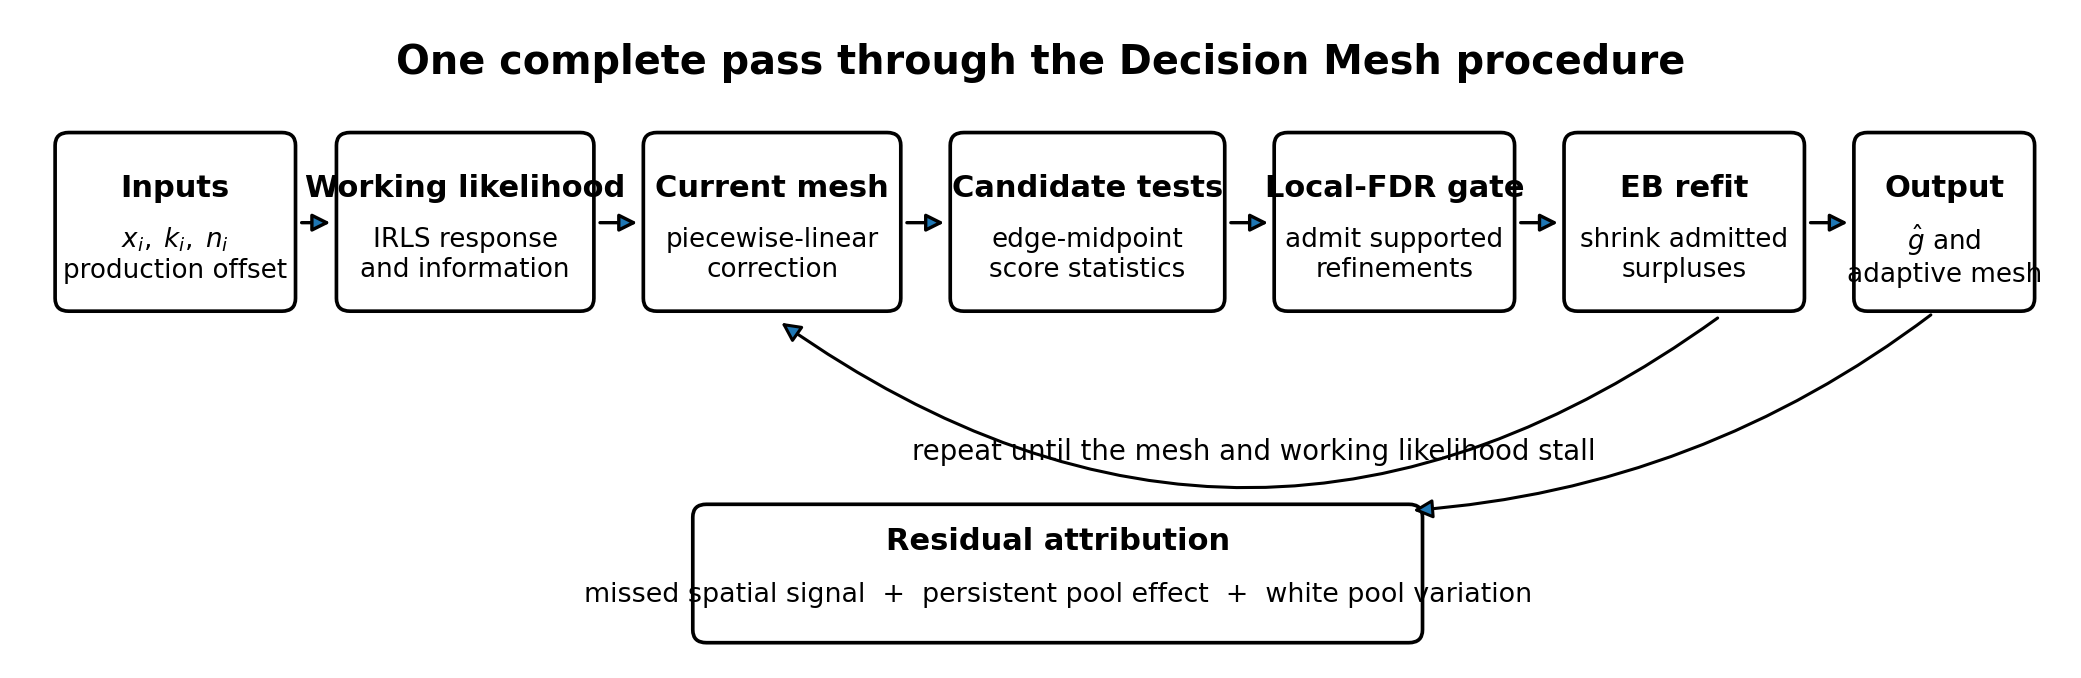
\includegraphics[width=\textwidth]{fig15_pipeline.png}
\caption{The complete Decision Mesh pipeline. The working likelihood and current mesh generate candidate edge-midpoint tests; an empirical-null local-FDR gate admits supported refinements; empirical-Bayes shrinkage stabilizes the added hierarchical coefficients. After the surface stalls, a separate moment layer attributes remaining variation to missed spatial signal and pool-level components.}
\label{fig:pipeline}
\end{figure}

\paragraph{Notation used throughout.}
\begin{center}\small
\begin{tabular}{ll@{\qquad}ll}
$x_i$ & pool coordinates (WALA, WAC) & $k_i,\,n_i$ & events and exposure\\
$\eta_{0,i}$ & production-model offset & $\hat g(x)$ & fitted correction surface (log-odds)\\
$u_P,\ \hat u_P$ & pool effect and its posterior mean & $\gamma$ & heavy-component responsibility\\
$(\pi,\sigma^2_{\mathrm{core}},\sigma^2_{\mathrm{tail}})$ & per-stratum pool law & $\sigma^2_a,\ \sigma^2_w$ & persistent and white residual variance\\
$w_i$ & binomial information $n_i p_i(1-p_i)$ & $c_i$ & likelihood temper / law discount\\
$K_{\mathrm{eff}}$ & effective pool support $(\sum\omega b)^2/\sum\omega^2 b^2$ & $T$ & trust $X^{\top}X/(X^{\top}X+\lambda)$\\
$\Delta$ & vertex surplus over parent interpolation & $\lambda_v$ & depth-specific EB precision\\
$z$ & calibrated gate score & $q$ & nominal FDR level\\
$\phi$ & dispersion estimate & $\varphi_j$ & temporal test functions (Sec.~\ref{sec:aug5-temporal})\\
\end{tabular}
\end{center}

\section{The current model, end to end}\label{sec:current}

This section is a self-contained mechanical specification of the recommended
configuration --- everything the fitted system does, in order, with the operative
formulas inline. Derivations, alternatives, and history live in the referenced
sections; nothing here requires them. The configuration is
\texttt{DMESH\_PL\_SOLVER=1},
\texttt{DMESH\_ONELAW=}$\langle$converged law$\rangle$,
\texttt{DMESH\_SIGMA0\_MIN=1.0}, FDR level $q=0.10$, with binomial-information
fitting weights throughout.

\paragraph{Formal objects.} Let $\mathcal{T}_0$ be the coarse conforming root
triangulation of the unit square and $\mathbb{T}$ the family of its conforming
newest-vertex-bisection refinements. For $T\in\mathbb{T}$, $V_T$ is the space of
continuous piecewise-linear functions on $T$ with nodal basis
$\{\phi_v\}_{v\in\mathcal{V}(T)}$. Every non-root vertex $v$ has edge parents
$p_0(v),p_1(v)$; writing $g=\sum_v h_v\phi_v$, the \emph{surplus} is
$\delta_v=h_v-\tfrac12(h_{p_0(v)}+h_{p_1(v)})$, and the \emph{hierarchical column}
of $v$ is the vector $b_{iv}=\psi_v(x_i)$ of its hierarchical basis function
evaluated at the data. The fitted model is the pair $(F,h)$ of a \emph{free set}
$F\subseteq\mathcal{V}(T)$ --- the admitted decisions --- and heights $h$, with
$\delta_v=0$ enforced for every conformity vertex $v\notin F$. Given working
weights $\omega_i$, tempers $c_i\in[0,1]$, and depth-specific precisions
$\lambda_v$, the height estimator at fixed $(T,F)$ is
\[
\hat h \;=\; \arg\max_{h:\,\delta_v=0\ \forall v\notin F}\;
\sum_i c_i\,\ell^{\mathrm{bin}}_i\bigl(\eta_{0,i}+g_h(x_i)\bigr)
\;-\;\tfrac12\sum_{v\in F}\lambda_v\,\delta_v^2 ,
\]
computed by exact one-dimensional coordinate maximization; the objective is
bounded above and ascent is monotone (derivation in
Section~\ref{sec:exactsolver}), which is the formal statement of eruption
impossibility. $X^\top X$ below always denotes $\sum_i\omega_i b_{iv}^2$ for the
candidate at hand, $K_{\mathrm{eff}}=(\sum_i\omega_i b_{iv})^2/\sum_i\omega_i^2
b_{iv}^2$, and $\kappa_{\mathrm{sc}}$ is the fixed internal variance-scale
constant converting law variances to working units. The mesh-growth procedure of
items 5--7 defines $(T,F)$ recursively: a candidate set of edge midpoints is
scored at the current $(T,F,\hat h)$, an admission set is chosen by the rule of
item 6, and the process repeats to a stall; the \emph{current model} is the
terminal $(T,F,\hat h)$ together with the pool-law posterior layer of item 9.

\begin{enumerate}[leftmargin=2em,itemsep=3pt]

\item \textbf{Inputs and scales.} Pools $i$ with coordinates $x_i$ (WALA, WAC,
rescaled to the unit square by fixed ranges), events and exposures $(k_i,n_i)$,
and the production offset $\eta_{0,i}$. Surface heights $h$ are carried in
centi-log-odds: the fitted log-odds at a pool is
$\eta_i=\eta_{0,i}+\hat g(x_i)$ with $\hat g$ the piecewise-linear element
function, internally $h/100$.

\item \textbf{Pool law.} \texttt{DMESH\_ONELAW} installs the converged
per-stratum two-normal mixture (strata by exposure: $<128$, $128$--$512$,
$512$--$4096$, $4096+$), as per-point variances $s^2_i$ (stratum totals
$0.143/0.242/0.029/0.004$ logit$^2$) and shape $s^4_i\kappa_i$ (excess
kurtosis $8.5/8.1/5.4/0$). The law prices admissions and attribution; it does
\emph{not} temper fitting weights.

\item \textbf{Working data.} Binomial information $w_i=n_ip_i(1-p_i)$ at the
current fit; working weights $1/(1/w_i+\xi_t)$ where $\xi_t$ is the stage
residual-dispersion extra; the likelihood temper $c_i$ is the ratio of working
weight to $w_i$. Held-out rows carry weight $\approx 0$ and never touch
sufficient statistics.

\item \textbf{Exact stage solver.} Active hierarchical coefficients are fitted
by coordinate ascent on the exact tempered penalized objective
$\sum_i c_i\,\ell^{\mathrm{bin}}_i(\eta_i) - \tfrac12\sum_v
\lambda_v\,(h_v-\bar h_v)^2$, each coordinate by an exact one-dimensional
profile ($\bar h_v$ is the parent-edge interpolation). The objective is
bounded and ascent monotone; the eruption mechanism of the legacy IRLS path
(Appendix~\ref{sec:boundary}) cannot occur.

\item \textbf{Candidate scoring.} Every admissible edge midpoint $v$ is scored
through its full hierarchical column: effect estimate $\hat\delta_v$ with
calibrated standard deviation
\[
\mathrm{sd}^2_{\mathrm{cal}}
=\Bigl(\frac{1}{X^\top X}
+\frac{\sum_i \kappa_{\mathrm{sc}}\, s^2_i\,\omega_i^2 b_i^2}{(X^\top X)^2}
+\rho\, s_p\Bigr)\,\hat\varphi ,
\]
the middle term the one-law composite null --- pool variance times the star's
concentration, so a one-pool-dominated star has an exploding null variance,
the continuous form of a minimum-effective-pools gate --- $\rho$ the parent
variance share, and $\hat\varphi$ the law-discounted Pearson dispersion
floored at 1. The candidate statistic is $z_v=\hat\delta_v/\mathrm{sd}_{\mathrm{cal}}$.
Effective support $K_{\mathrm{eff}}=(\sum\omega b)^2/\sum\omega^2b^2$ is
recorded and re-checked at commit.

\item \textbf{Empirical null and admission.} The candidate family's $z$'s are
pooled; a Lindsey log-spline density estimate with central matching fits the
null $(\delta_0,\sigma_0,\pi_0)$ under the constraints $\sigma_0\in[1,1.4]$
(the floor is load-bearing: one-law pricing deflates the null bulk on
variance the data may not carry, and an unfloored match flags the least
deflated candidates), $\pi_0\ge 0.05$. With $f$ the Lindsey estimate of the pooled $z$ density and
$f_0=\mathcal{N}(\delta_0,\sigma_0^2)$ the matched null, the admission set is
the largest prefix of candidates ordered by
$\mathrm{lfdr}(z)=\pi_0 f_0(z)/f(z)$ whose running mean lfdr is at most
$q=0.10$:
\[
A=\Bigl\{v_{(1)},\dots,v_{(m^*)}\Bigr\},\qquad
m^*=\max\Bigl\{m:\ \tfrac1m\textstyle\sum_{j\le m}
\mathrm{lfdr}\bigl(z_{(j)}\bigr)\le q\Bigr\}.
\] Root scales are never thresholded. Measured size: 0.2--0.3
false admissions per run on flat-marginal true nulls
(Section~\ref{sec:aug5}).

\item \textbf{Refinement.} Admitted vertices activate; newest-vertex
bisection cascades restore conformity, conformity vertices carrying the
parent interpolation with zero degrees of freedom; the exact solver refits;
rounds repeat until the mesh stalls across the declared stages.

\item \textbf{Shrinkage and finish.} Each free surplus carries a
depth-specific empirical-Bayes prior centered on parent interpolation with
precision $\lambda_v$ estimated from the depth ladder; trust
$T=X^\top X/(X^\top X+\lambda_v)$ is reported per vertex and is only
interpretable jointly with $K_{\mathrm{eff}}$. At fixed topology a final
re-shrink pass runs, and coefficients whose hierarchical columns are zero on
the training design are retired under the retirement audit.

\item \textbf{Outputs and attribution.} The surface $\hat g$; per-pool
posterior effects under the law, $\hat u_P$ and heavy responsibility
$\gamma_P$, by adaptive Gauss--Hermite over the two components; and the
residual ledger. The EM mixture law is the primary variance instrument; the
PM/energy moment instruments carry a measured $\sim3.5\times$ upward bias
under heavy tails and an exact clean-null falsification
(Section~\ref{sec:aug5}).

\end{enumerate}

Not part of the current model: law-tempered fitting weights (retired,
double-charging), the two-currency final temper and the law-marginal final
pass (both implemented, measured, and experimental), and the temporal layer
(designed, Section~\ref{sec:aug5-temporal}).

\section{Statistical model and effective exposure}\label{sec:model}

Data are indexed by $i=1,\dots,N$, each observation a pool-month:
covariate location $x_i\in\Omega\subset\mathbb{R}^2$ (for the motivating application
$x=(\text{WALA},\text{WAC})$ after affine rescaling of the axes to comparable ranges),
exposure $n_i$, event total $k_i$, and a known offset $\eta_{0,i}$ produced by an
existing (``internal'') model, possibly including known per-observation log-odds shifts
from observed characteristics. For literal loan-count outcomes, $n_i$ and $k_i$ are
integer counts. For balance-weighted outcomes they may instead be continuous
variance-matching pseudo-counts, as described below. The baseline generative model is
\begin{equation}\label{eq:model}
k_i \mid u_i \sim \mathrm{Binomial}\bigl(n_i,\ p_i\bigr),\qquad
\logit p_i = \eta_{0,i} + g(x_i) + u_i,
\end{equation}
where $g:\Omega\to\mathbb{R}$ is the unknown correction surface (log-odds units) and
$u_i$ is a mean-zero random effect representing unobserved variables,
$\Var(u_i)=\sigma_u^2$. The target of estimation is $g$; the targets of the diagnostic
layer (Section~\ref{sec:attribution}) are $\sigma_u^2$ and the energy of whatever part of $g$
the fit has missed.

\subsection{Continuous effective exposure for balance-weighted outcomes}
\label{sec:wacls}

The binomial representation is literal when the response is a loan count.  A
balance-weighted prepayment rate has a different sampling variance when loan
sizes differ.  Let the current balances in a pool be $b_1,\ldots,b_m$, let
$I_j\in\{0,1\}$ indicate whether loan $j$ prepays over the observation period,
and suppose first that the loans share a common conditional prepayment
probability $p$.  The prepaid balance is
\[
K_B=\sum_{j=1}^m b_j I_j,
\qquad
\Var(K_B\mid b)=p(1-p)\sum_{j=1}^m b_j^2.
\]
Define the weighted-average current loan size
\[
\mathrm{WACLS}=\frac{\sum_j b_j^2}{\sum_j b_j}.
\]
The variance-matching effective exposure and event equivalent are then
\begin{equation}\label{eq:wacls-counts}
 n_{\mathrm{eff}}
 =\frac{\sum_j b_j}{\mathrm{WACLS}}
 =\frac{(\sum_j b_j)^2}{\sum_j b_j^2},
 \qquad
 k_{\mathrm{eff}}
 =\frac{\sum_j b_j I_j}{\mathrm{WACLS}}.
\end{equation}
They satisfy $\E[k_{\mathrm{eff}}\mid b]=n_{\mathrm{eff}}p$ and
$\Var(k_{\mathrm{eff}}\mid b)=n_{\mathrm{eff}}p(1-p)$ exactly.  Thus
$(k_{\mathrm{eff}},n_{\mathrm{eff}})$ has the first two moments of a binomial
observation even though neither quantity need be an integer.  The fitting
criterion
\[
\ell(\eta)=k_{\mathrm{eff}}\eta-n_{\mathrm{eff}}\log(1+e^\eta)
\]
is therefore used as a quasi-binomial log likelihood.  All score, IRLS, and
Pearson-residual formulas below remain unchanged after replacing $(k_i,n_i)$
by continuous $(k_{\mathrm{eff},i},n_{\mathrm{eff},i})$.

The effective count is the inverse Herfindahl concentration of current loan
balances.  Equal-sized loans give $n_{\mathrm{eff}}=m$; concentration in a few
large loans reduces the information.  For loan-size coefficient of variation
$c_v$ and a moderately large pool,
$n_{\mathrm{eff}}/m\approx(1+c_v^2)^{-1}$.  Dividing prepaid balance by the
ordinary average loan size while retaining the literal loan count therefore
understates the variance by approximately $1+c_v^2$.  Equation
\eqref{eq:wacls-counts} is intended for balance-weighted outcomes only; when
actual loan counts are observed, the disclosed count remains preferable.

\begin{figure}[ht]
\centering
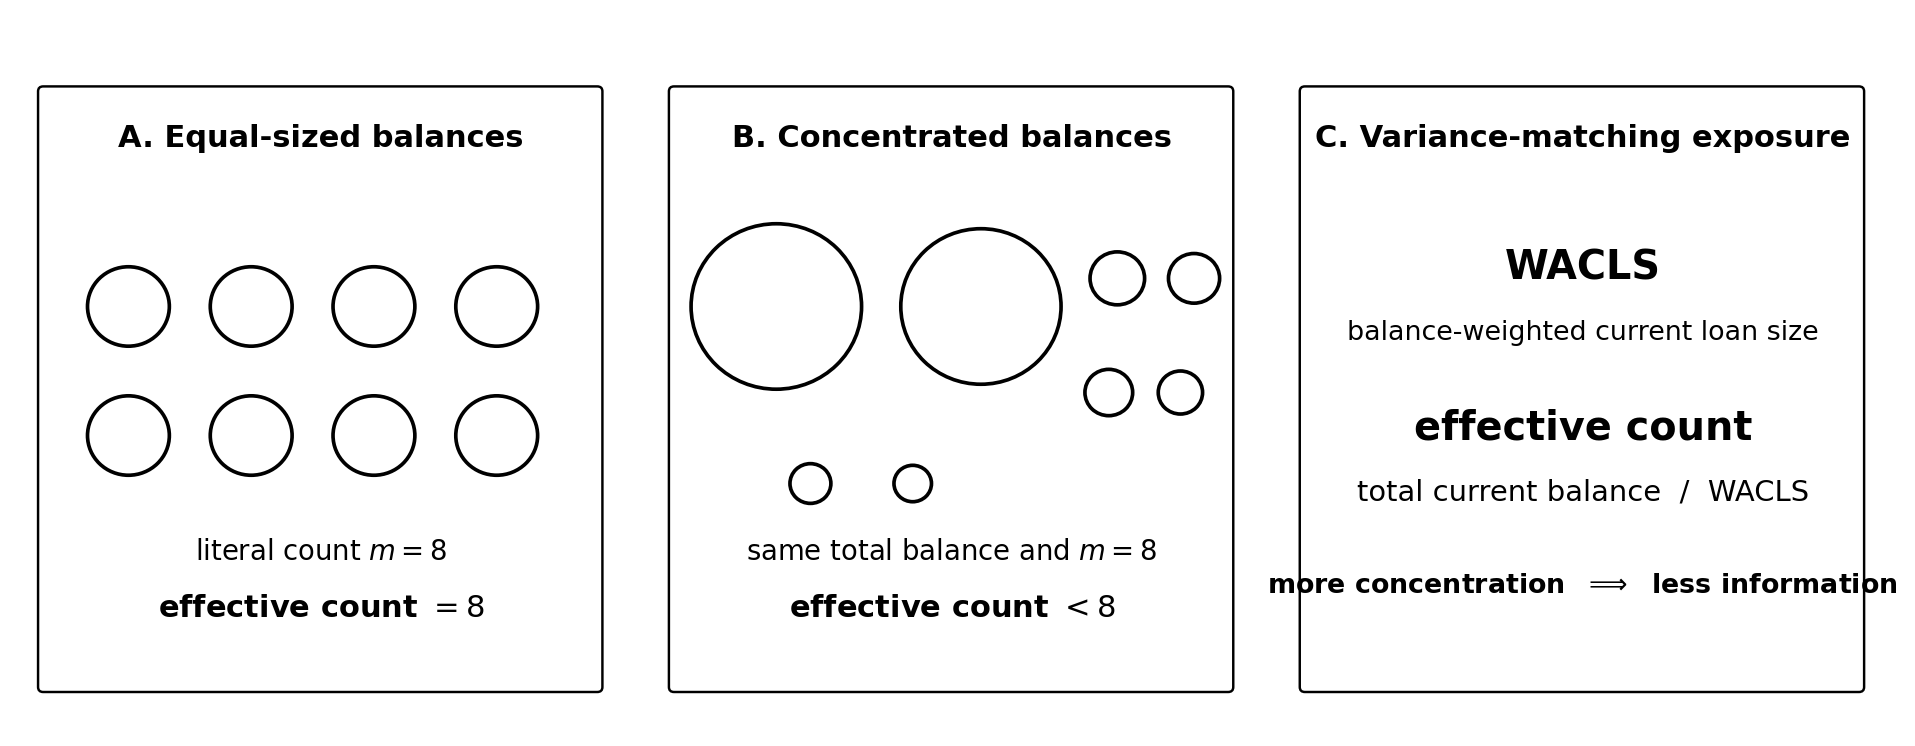
\includegraphics[width=0.96\textwidth]{fig19_wacls_effective_count.png}
\caption{Why balance-weighted outcomes require an effective exposure. Equal-sized loans preserve the literal count, while concentration of the same total balance in a few large loans reduces the variance-matching exposure. The WACLS formula is the inverse concentration of current balances and exactly matches the first two moments when loans share a conditional event probability.}
\label{fig:wacls-concept}
\end{figure}

Two features of the application drive the design. First, the support of the sampling
distribution is a union of cohort trajectories: at any calendar month each loan age is
occupied by exactly one vintage, so cross-sections are one-dimensional curves and the
two-dimensional support is swept out over time. Large regions of $\Omega$ are
structurally empty and must never receive confident extrapolation. Second, the
correction is a \emph{deliverable against a production model}: every basis function that
exists in $\hat g$ should be individually certified, and the default in the absence of
evidence must be $\hat g=0$.


\begin{figure}[h]
\centering
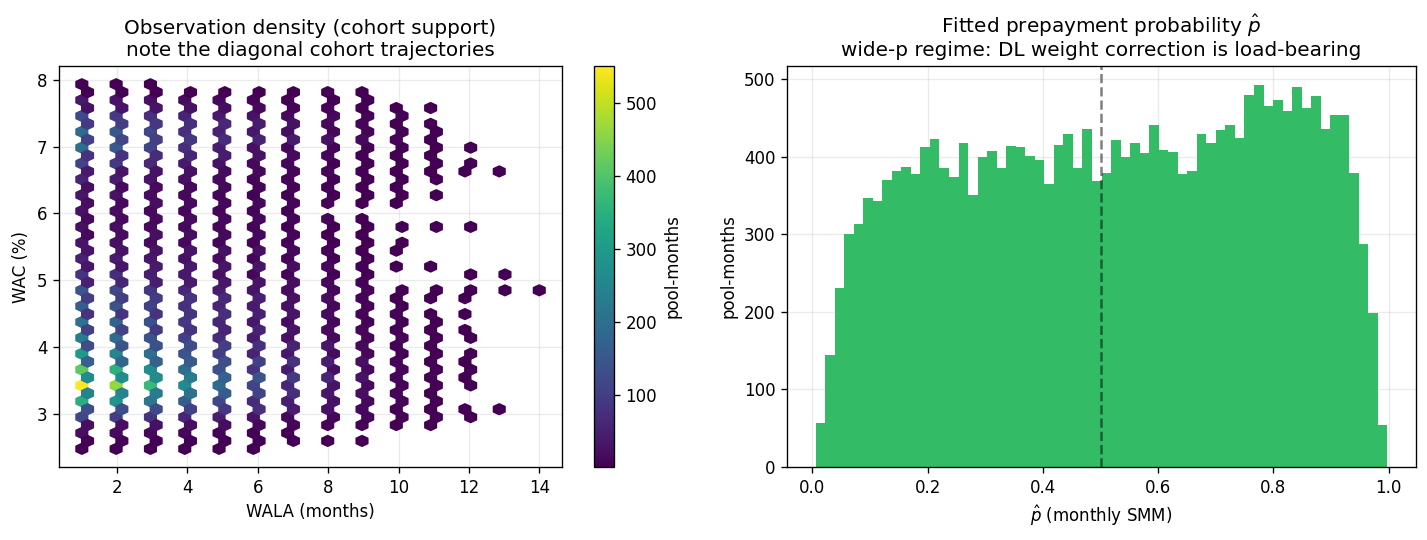
\includegraphics[width=\textwidth]{fig2_data.png}
\caption{The simulated data regime. Left: observation density in $(\text{WALA},\text{WAC})$ under cohort dynamics; support is confined to diagonal cohort trajectories and dies with attrition. Right: fitted $\hat p$ spans essentially $(0,1)$ (the wide-$p$ regime), which is what makes the re-expansion of Section~\ref{sec:glm} and the $(1-2\hat p)$ terms of Section~\ref{sec:attribution} load-bearing.}
\label{fig:data}
\end{figure}

\noindent\textbf{Assumption (no common calendar shocks).} The model contains
no calendar-time effects: conditional on $(\text{WALA},\text{WAC})$ and the
pool effects, observations in the same calendar month are independent. Real
prepayment data violates this; rate-path surprises, seasonality, and media
effects are common monthly shocks, neither i.i.d.\ pool noise nor functions
of the coordinates; and because pools in a cell are largely observed in
the same months (vintage and coupon are correlated), such shocks load onto
the cross-pool moments and, if serially correlated, contaminate the pool
moments. This assumption is stated as a limitation: the simulator cannot
reveal the violation on its own because its generator matches the model, and
calendar-month intercepts in the fit (standard in production prepayment
models) are the appropriate extension when multi-month real panels are in
scope.

\paragraph{Status and reproducibility.} Simulation claims in this document
are labeled with their seed counts; unlabeled figures are single-seed
illustrations, and every estimator-level claim rests on three to ten seeds
as stated at the point of use. Section~\ref{sec:conditionality} tabulates
which inferential outputs are conditional on which estimated quantities;
claims should be read against that table.

\section{Likelihood and one-step scoring}\label{sec:glm}

\subsection{Offset GLM and IRLS}
Conditional on $u\equiv 0$, \eqref{eq:model} is a binomial GLM with offset $\eta_0$ and
linear predictor $\eta_i=\eta_{0,i}+\sum_v h_v\varphi_v(x_i)$. Fisher scoring for the
log-likelihood $\ell(h)=\sum_i k_i\eta_i-n_i\log(1+e^{\eta_i})$ is iteratively
reweighted least squares on the working response and weights
\begin{equation}\label{eq:working}
y_i \;=\; \hat g^{(m)}(x_i)+\frac{k_i-n_i p_i^{(m)}}{n_i p_i^{(m)}q_i^{(m)}},
\qquad
w_i \;=\; n_i p_i^{(m)} q_i^{(m)},
\qquad p_i^{(m)}=\sigma\!\bigl(\eta_{0,i}+\hat g^{(m)}(x_i)\bigr),
\end{equation}
with $q=1-p$ and $\sigma$ the logistic function. The inner problem at each outer
iteration $m$ is weighted least squares in the P1 basis; at a fixed point the heights
satisfy the binomial score equations, so the estimator is maximum (penalized) likelihood
implemented on a WLS engine. In practice one outer step at the internal model
($m=0$, $\hat g^{(0)}=0$) captures most of the correction and outer refreshes are
applied whenever the refinement gate stalls.

\begin{proposition}[first-order unbiasedness of one-step scoring]\label{prop:onestep}
Let $\logit p=\eta_0+\delta$ and $y=(k-np_0)/(np_0q_0)$ with $p_0=\sigma(\eta_0)$. Then
$\E[y]=\delta+O(\delta^2)$ and $\Var(y)=1/(np_0q_0)+O(\delta)$.
\end{proposition}

\emph{Adequacy criterion.} The $O(\delta^2)$ bias coefficient
$\tfrac12(1-2p_0)$ is $\approx\tfrac12$ at hazard scale, so a correction of
$0.8$ log-odds carries a first-round bias near $0.3$: one-step is a
coarse-regime device. The operational criterion used throughout is: one-step
is adequate while the largest admitted surplus per round stays below
$\sim0.5$ log-odds; beyond that, the IRLS re-expansion (every third round and
on stall) re-linearizes, and the wide-$p$ regimes in this document always run
with re-expansion on. No claim is made for one-step alone outside that
envelope.
\begin{proof}
$\E k=np(\delta)$ and $p(\delta)=p_0+p_0q_0\delta+O(\delta^2)$ by
$dp/d\eta=pq$; divide by the information $np_0q_0$. The variance statement follows from
$\Var k=np(\delta)q(\delta)$.
\end{proof}

\subsection{Exact tempered penalized coordinate ascent}\label{sec:exactsolver}
The IRLS construction above remains useful for diagnostics and for the legacy gate, but it is no
longer the stage height solver on the development line. Let $c_i\in(0,1]$ be the current
pool-law tempering factor and let $\lambda_{d(v)}$ be the precision of the depth-specific Gaussian
hierarchical prior. With prior targets $m_v$ held fixed during a sweep, the stage objective is
\begin{equation}\label{eq:exact-objective}
Q(h)=\sum_i c_i\left[k_i\eta_i-n_i\log(1+e^{\eta_i})\right]
-\frac12\sum_{v\in V_{\mathrm{free}}}\lambda_{d(v)}(\delta_v-m_v)^2,
\qquad
\eta_i=\eta_{0,i}+\hat g_h(x_i).
\end{equation}
For coordinate $v$, the solver maximizes the concave one-dimensional function
$Q_v(a)=Q(h+a e_v)$ by safeguarded Newton steps and accepts an update only when the full objective
is nondecreasing. The same hierarchical column engine is used by the stage solver, candidate
profiler, information census, and retirement pass.

This change removes the eruption mechanism rather than merely clipping it. A saturated binomial
likelihood may have tiny local Fisher curvature, so a stale quadratic can propose an enormous move;
the exact objective still has a finite penalized optimum and a finite gain. In the B1 closure tests,
thousands of committed coordinates were reprofiled against the full objective with zero failures,
and the stored gain and realized objective increase agreed to roughly $10^{-10}$ nats. After removal
of the now-dead saturation fallback, a 20-split battery had zero eruptions, mean held-out NLL
$2.9449$, standard deviation $0.0054$, and worst split $2.9537$.

\subsubsection{Coupled hierarchical penalties and stationarity}
The implementation stores canonical vertex heights $h$, while the Gaussian prior is placed on
hierarchical surpluses. Write the free-surplus vector as
\[
\delta=Ah,
\qquad
P(h)=\frac12(Ah-m)^\top\Lambda(Ah-m),
\]
where a row of $A$ is the midpoint surplus map: its own height has coefficient $1$ and its two
parent heights have coefficient $-1/2$, with inherited parent representations expanded through
constrained vertices. The correct prior gradient and Hessian are therefore
\begin{equation}\label{eq:coupled-prior-gradient}
\nabla P(h)=A^\top\Lambda(Ah-m),
\qquad
\nabla^2P(h)=A^\top\Lambda A.
\end{equation}
A coordinate move in a parent height changes not only that vertex's own surplus but also every free
descendant surplus whose inherited parents contain the moved coordinate. Pricing only the visited
vertex's diagonal term omits the off-diagonal entries of $A^\top\Lambda A$ and can converge to a
fixed point of the implemented updates while the gradient of \eqref{eq:exact-objective} remains
nonzero.

The corrected solver constructs, once per stage fit, the sparse derivative of every penalized
surplus with respect to every canonical free height. During Gauss--Seidel sweeps it updates both the
likelihood predictions and the affected prior residuals. Thus the one-dimensional Newton profile for
coordinate $j$ uses
\[
\frac{d}{da}P(h+a e_j)
=(Ae_j)^\top\Lambda\{Ah-m+a(Ae_j)\},
\]
rather than only the coordinate's own prior term. This is a correction to the objective evaluation,
not a switch to surplus coordinates; an exact reparameterization to $\delta$ would leave the fitted
surface and NLL unchanged on fixed topology.

On the final Ginnie fit, 1,256 nonroot coordinates were audited. Of the 1,255 interior coordinates,
the maximum absolute full-objective gradient was $3.65\times10^{-6}$ nats per logit and the RMS was
$1.64\times10^{-7}$; one coordinate lay at the $-12$ logit cap and there were no boundary KKT
violations. The predictive comparison is
\begin{center}
\begin{tabular}{@{}lr@{}}
\toprule
Variant & marginal held-out NLL\\
\midrule
Release baseline & $2.9410$\\
Stage-initial exact fit with diagonal-only prior update & $2.9520$\\
Stage-initial exact fit with coupled hierarchical penalties & $2.9443$\\
\bottomrule
\end{tabular}
\end{center}
The coupled correction recovers about $70\%$ of the deterioration introduced by enabling the
previously skipped stage-initial exact fit. It improves the ramp-region NLL and ordinary held-out
deviance relative to the diagonal-only exact fit, but does not beat the release baseline overall;
the seasoned-region marginal NLL is slightly worse. The correction is retained because it makes the
solver stationary for its stated objective, not because it establishes a new predictive optimum.

\subsection{Why the empirical logit must not be used}\label{sec:empiricallogit}
The classical alternative response, the Haldane--Anscombe empirical logit
$\tilde y=\log\{(k+\tfrac12)/(n-k+\tfrac12)\}$ with Gart variance
$(k+\tfrac12)^{-1}+(n-k+\tfrac12)^{-1}$, is designed for $npq$ moderately large. At
prepayment scale ($p\sim 0.2$--$2\%$ monthly, $n$ of order $10^2$) it fails for two
compounding reasons. (i) \emph{Floor}: $\tilde y\ge \log\{0.5/(n+0.5)\}$
($=-6.22$ at $n=250$) regardless of how small $p$ is, and the flooring event $k=0$ is
the modal outcome; e.g.\ at $np=1$, $P(k{=}0)\approx e^{-1}\approx 0.37$. (ii)
\emph{Outcome-dependent weights}: the Gart precision is approximately $k+\tfrac12$, so
observations that randomly realized more events receive both larger $\tilde y$ and more
weight, biasing any precision-weighted average upward. In the development simulation the
combined bias of the precision-weighted mean was $\approx +0.5$ log-odds against a truth
of $-0.82$; the mesh reproduced its (biased) target almost exactly, capping recoverable
signal at $59\%$, versus $93$--$94\%$ under one-step scoring. The one-step construction
\eqref{eq:working} has no floor (a $k=0$ month contributes a mildly negative residual)
and its weights are functions of the model, not of $k$.

\begin{remark}[the $+\tfrac12$ in its proper place]
Regularization against separation is still required at the \emph{likelihood} level: a
vertex whose entire star contains only $k=0$ observations has a monotone likelihood and
unpenalized ML sends $h_v\to-\infty$, dragging every adjacent face with it because the
basis is continuous. Firth's bias-reduction penalty (the Jeffreys prior) is the
principled fix \cite{firth1993}; on a single binomial cell it reduces exactly to adding
$\tfrac12$ to each count. Applied once, at the likelihood, on pooled counts, the idea is
correct; applied per observation to a plug-in estimator with outcome-dependent weights,
it is the failure described above. In the implementation the empirical Bayes prior of
Section~\ref{sec:eb} supplies the penalty.
\end{remark}

\section{Overdispersion and known covariates}\label{sec:overdisp}

\subsection{Random effects in $p$}
With $u_i$ present, the working residual has variance $1/w_i+\sigma_u^2$, so the
efficient weights are the DerSimonian--Laird weights
\begin{equation}\label{eq:dlw}
\tilde w_i=\Bigl(\frac{1}{w_i}+\sigma_u^2\Bigr)^{-1}\ \le\ \frac{1}{\sigma_u^2}.
\end{equation}
The saturation bound is operationally decisive for MBS data, where $n$ spans single
digits (small spec pools) to $10^5$ (Ginnie~II multi-issuer): a mega-pool with
$w=npq\approx 10^3$ carries $\tilde w\approx 1/\sigma_u^2\approx 11$ at
$\sigma_u=0.3$, i.e.\ is worth only a few hundred-loan pools; cross-sectional pool
count, not loan count, drives precision. Uncorrected, mega-pool null $z$'s are inflated
by $\sqrt{1+w\sigma_u^2}$, far beyond the empirical null's constraint, and the gate
over-refines into $u$-noise. At small $w\sigma_u^2$ (the homogeneous-$n$ simulations,
inflation $\approx 11\%$) the constrained empirical null absorbs the effect and the
correction is nearly redundant; heterogeneity in $w$ is what makes it load-bearing.

\subsection{Known log-odds shifts}
A characteristic $c_i$ with \emph{known} coefficient enters the offset,
$\eta_{0,i}\mapsto\eta_{0,i}+\beta c_i$; the entire pipeline is invariant to it (weights
become heteroskedastic per observation, which the weighted face statistics carry
through). If instead the shift is omitted, it is independent of location and therefore
statistically indistinguishable from $u$:

\begin{proposition}[misspecification identity]\label{prop:audit}
If a known shift $\beta c_i$, $c_i\perp x_i$, $\Var(c)=1$, is omitted from the offset,
the idiosyncratic moment of Section~\ref{sec:attribution} estimates
$\sigma_u^2+\beta^2$ in place of $\sigma_u^2$.
\end{proposition}

\noindent This yields two tools: an \emph{audit} (measured $\sigma_u^2$ above what is
plausible for genuine unobservables quantifies characteristics missing from the
offset) and a \emph{valuation statistic} (the drop in $\hat\sigma_u^2$ when a candidate
adjustment is added to the offset is the log-odds variance that characteristic
explains). A current exact/quadratic five-seed rerun gives mean leverage-corrected estimates
$0.09106$ with the shift in the offset and $0.20512$ when it is omitted, against targets
$0.0900$ and $0.0900+0.35^2=0.2125$. The matched increment is $0.11406$, recovering
$93.1\%$ of the theoretical omitted contribution $0.35^2$. The seed standard deviations are
$0.00378$ and $0.00376$, respectively. All ten fits completed successfully.


\begin{figure}[ht]
\centering
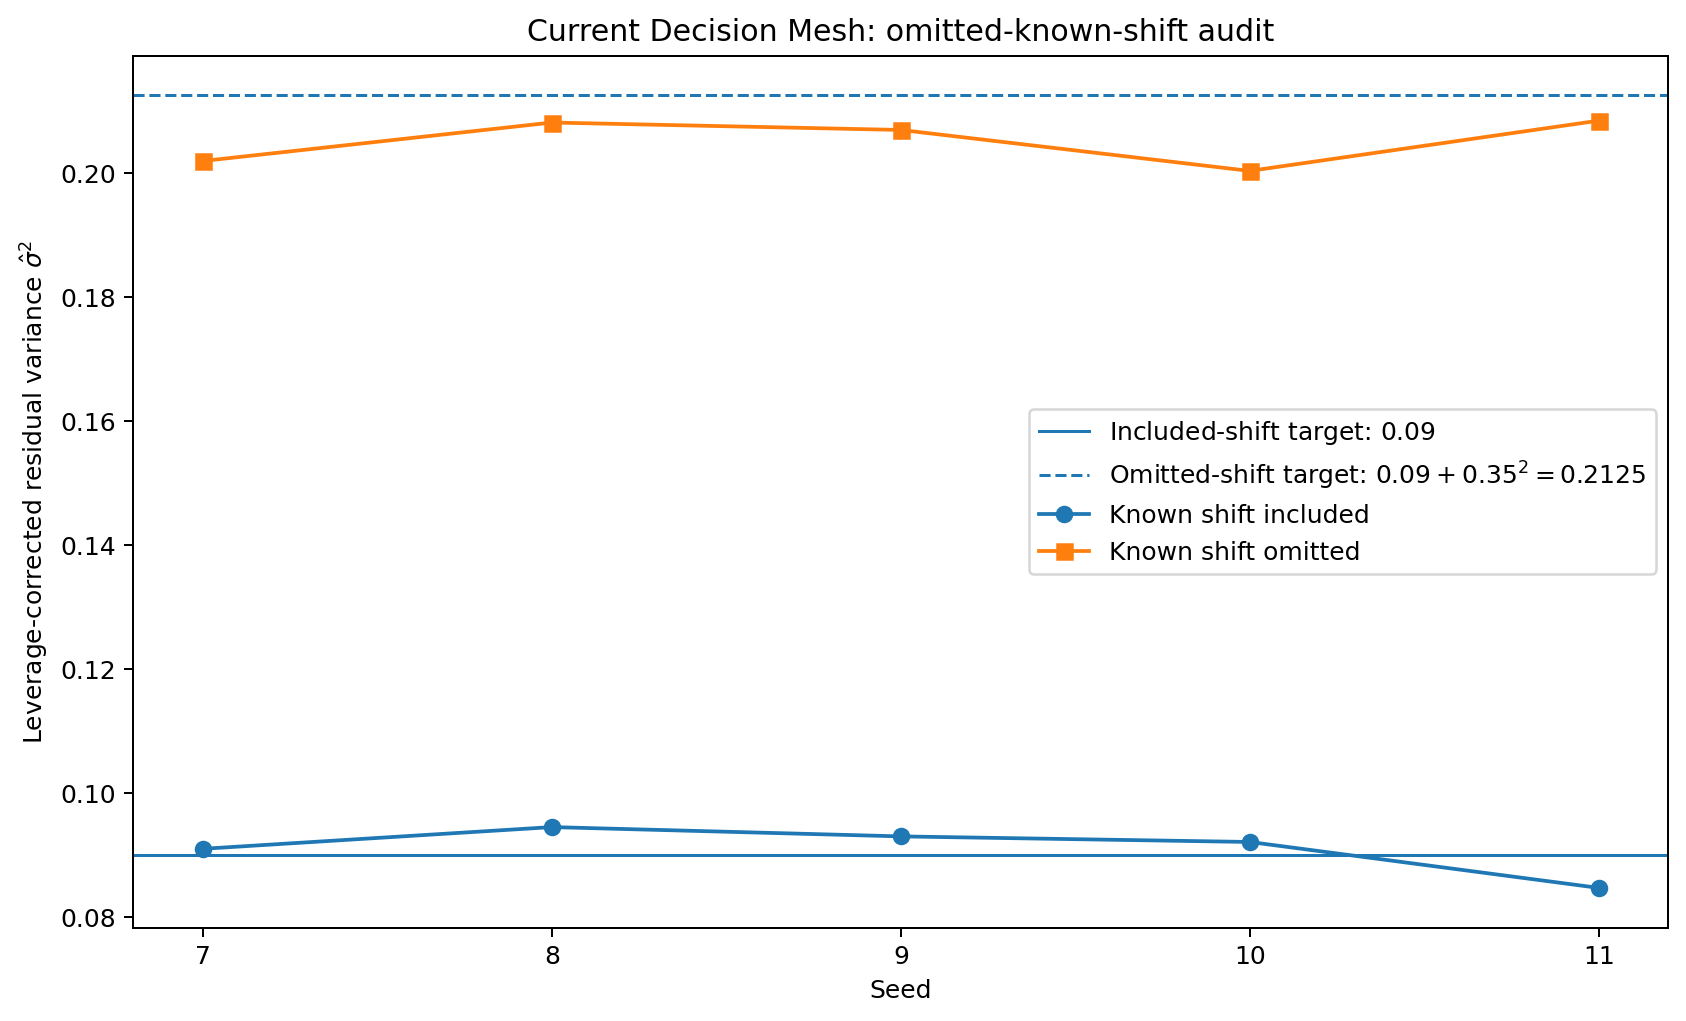
\includegraphics[width=0.78\textwidth]{current_known_shift_audit.png}
\caption{Current-estimator omitted-known-shift audit, five matched seeds. With the known
$0.35$ log-odds shift included, the residual-variance estimate is centered near $0.09$; when
it is omitted, the estimate rises toward $0.09+0.35^2=0.2125$. The matched increment
recovers $93.1\%$ of the omitted variance contribution.}
\label{fig:current-known-shift}
\end{figure}

\section{Adaptive finite-element representation}\label{sec:representation}

\subsection{Newest vertex bisection}
$\Omega$ is triangulated starting from two right triangles obtained by splitting the
bounding box along a diagonal. Refinement is by newest vertex bisection (NVB): each
triangle carries a refinement edge (the edge opposite its newest vertex); activating the
midpoint $v$ of an edge $e$ bisects $e$ and both adjacent triangles along the chord from
$v$ to each opposing vertex. If a triangle is asked to split along a non-refinement
edge, a completion cascade first bisects it along its own refinement edge, recursively;
the mesh therefore remains conforming at all times \cite{mitchell1991,binev2004}. Under
NVB all triangles produced from a right isosceles initial mesh belong to a finite set of
similarity classes, so shape regularity (minimum angle bounded away from zero) holds
uniformly at every depth; this is why the axes must be pre-scaled: on a raw domain of
aspect ratio $\sim 14$, every admissible bisection violates the shape guard and
refinement cannot start.

Point location is by a binary tree recording, at each internal node, the separating
line between its two children. The separating line of an NVB split is the \emph{chord}
(midpoint to opposing vertex), not the bisected edge; the parent face lies entirely on
one side of the line containing its own edge, so storing the edge yields a walk that is
deterministic and wrong at every non-root node. With the chord stored, prediction is an
$O(\log F)$ walk followed by barycentric interpolation.

\subsection{Basis and surplus coefficients}
Write $V$ for the active vertices and $\{\varphi_v\}_{v\in V}$ for the continuous
piecewise-linear (P1) hat functions on the current mesh, $\varphi_v(v')=\delta_{vv'}$.
The fitted surface is $\hat g(x)=\sum_{v} h_v\varphi_v(x)$. For a midpoint $v$ of edge
$e=(p_0,p_1)$, define the \emph{linear interpolant value}
$\mu_{\mathrm{lin}}(v)=\tfrac12(h_{p_0}+h_{p_1})$ and the \emph{surplus} (hierarchical
coefficient)
\begin{equation}\label{eq:surplus}
\delta_v \;=\; h_v-\mu_{\mathrm{lin}}(v).
\end{equation}
Activating $v$ adds exactly one degree of freedom, and $\delta_v=0$ reproduces the
pre-split surface; the hierarchy $\{\delta_v\}$ plays the role of wavelet coefficients
in \cite{abramovich2006}, which is the closest antecedent of the gating idea below.

\begin{figure}[ht]
\centering
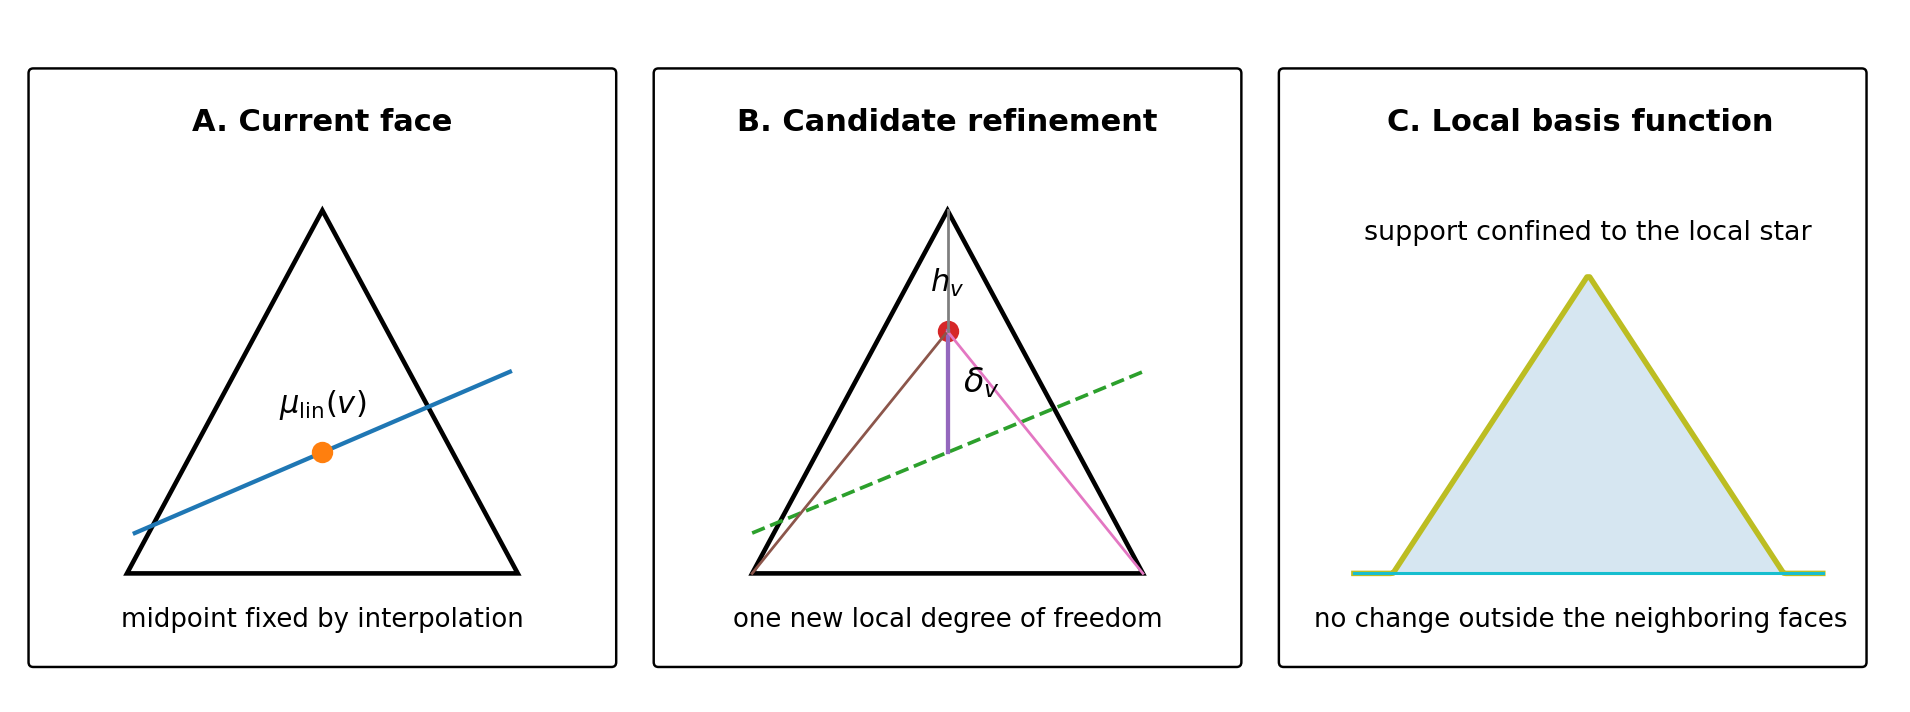
\includegraphics[width=\textwidth]{fig16_hierarchical_surplus.png}
\caption{The hierarchical coefficient tested by a candidate edge split. Before refinement the midpoint value is fixed by interpolation between its parents. Activating the midpoint adds one local degree of freedom, the surplus $\delta_v=h_v-\mu_{\mathrm{lin}}(v)$; setting $\delta_v=0$ exactly reproduces the pre-split surface.}
\label{fig:surplus-concept}
\end{figure}

\subsection{Geometry, statistical freedom, and hierarchical support}\label{sec:lifecycle}
A vertex can exist geometrically without carrying an independent coefficient. This distinction is
necessary because NVB conformity cascades create midpoint vertices that are required by the mesh but
were not themselves admitted by the gate. The implementation therefore distinguishes:
\begin{enumerate}[leftmargin=2em,itemsep=1pt]
\item \emph{geometry-only or constrained}: the vertex exists and its surplus is fixed at zero;
\item \emph{free}: the surplus is an optimized statistical coordinate;
\item \emph{dormant}: a free coordinate currently has negligible likelihood information but is not
structurally absent;
\item \emph{retired}: at fixed topology the coordinate has been proved to have zero training support
and is returned to zero surplus.
\end{enumerate}

For a free coefficient $v$, define its hierarchical design column
\begin{equation}\label{eq:hiercol}
X^H_{iv}=\frac{\partial \hat g(x_i)}{\partial \delta_v}.
\end{equation}
The derivative propagates through constrained descendants and stops when it reaches another free
coefficient. It is therefore generally different from the nodal P1 hat function. Structural support,
likelihood information, and replication are separate quantities:
\begin{equation}\label{eq:support-info}
S_v^{\mathrm{geom}}=\sum_{i\in\mathcal T}(X^H_{iv})^2,
\qquad
I_v=\sum_{i\in\mathcal T} c_i n_i p_i(1-p_i)(X^H_{iv})^2,
\end{equation}
where $\mathcal T$ is the explicit training split. Retirement uses only
$S_v^{\mathrm{geom}}$: small $I_v$ makes a coordinate imprecise, and low effective pool count makes
it difficult to certify, but neither makes the coordinate geometrically nonexistent.

Retirement is performed deepest first, rebuilding the hierarchy after each depth batch. Before any
post-retirement refit, each batch must leave all training predictions invariant to numerical
precision. On the original-split B1 regression this rule retired $67$ genuinely empty columns,
rescued $12$ vertices that were nodally empty but hierarchically supported, and changed the training
predictor by exactly zero before reoptimization. The previous nodal-star cleanup had incorrectly
retired supported ancestors and moved some predictions by several logits.

\begin{figure}[ht]
\centering
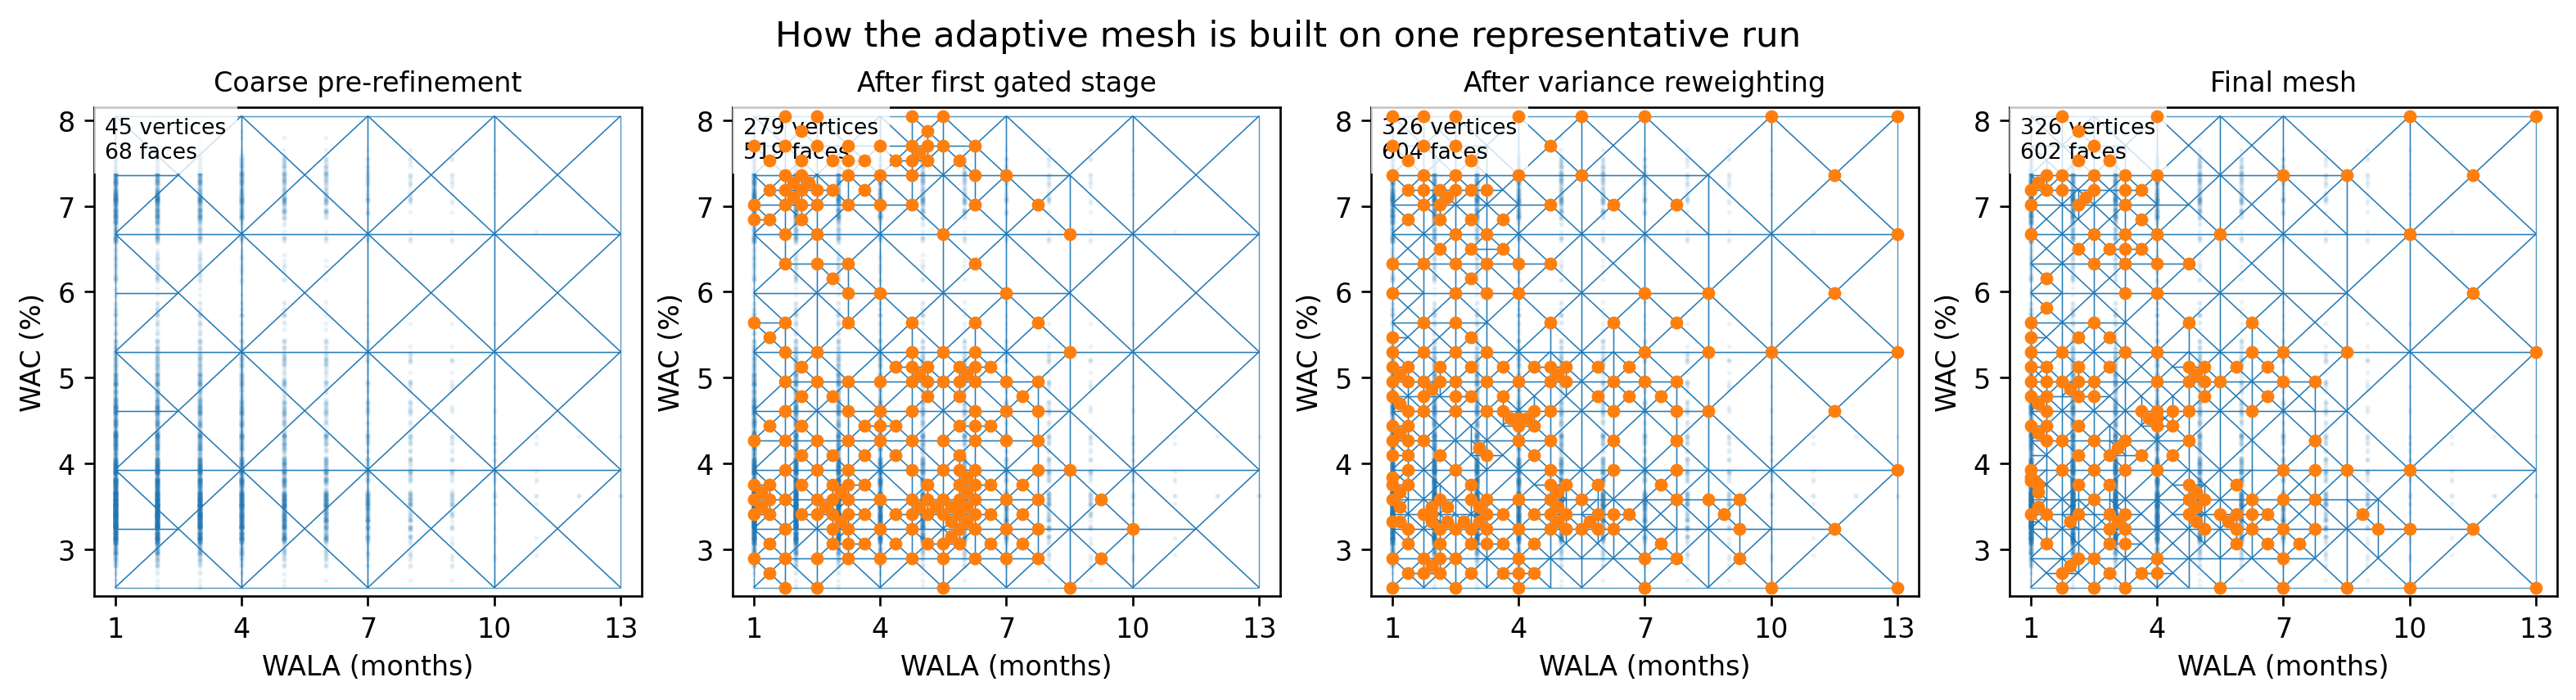
\includegraphics[width=\textwidth]{fig20_mesh_build_progression.png}
\caption{Mesh construction across the three outer fitting stages for one representative continuous-WACLS run. The first panel is the common pre-refined mesh. Colored points in later panels mark vertices added since the preceding panel. Refinement remains concentrated on observed support, while variance reweighting between stages changes which local deviations remain worth resolving.}
\label{fig:mesh-build}
\end{figure}

\section{Local-FDR-gated refinement}\label{sec:gate}

Each inactive midpoint $v$ (a candidate refinement) is a hypothesis
\[
H_0(v):\ \delta_v=0 \quad\text{(the surface is linear across edge $e(v)$)} .
\]
Fixing all other heights, the coordinate-wise WLS estimate of $h_v$ over the (simulated)
star of $v$ is
\begin{equation}\label{eq:coord}
\hat\beta_v=\frac{x^\top W r}{x^\top W x},\qquad
x=(\varphi_v(x_i))_i,\ \ W=\mathrm{diag}(w_i),\ \
r_i=y_i-\!\!\sum_{u\neq v}\!h_u\varphi_u(x_i),
\end{equation}
with conditional variance $\sigma^2/(x^\top Wx)$, where $\sigma^2$ is the working-scale
noise ($\sigma=1$ when $w$ carries the full precision, as in \eqref{eq:working}).

\subsection{Exact candidate gain and its signed-root coordinate}\label{sec:exactgain}
For an inactive candidate, let $X^H_v$ be the hierarchical column it would acquire upon activation
and profile the exact objective \eqref{eq:exact-objective} while holding the existing coordinates
fixed:
\begin{equation}\label{eq:exactgain}
\hat a_v=\arg\max_a Q_v(a),
\qquad
\Delta Q_v=Q_v(\hat a_v)-Q_v(0),
\qquad
r_v=\operatorname{sign}(\hat a_v)\sqrt{2\Delta Q_v}.
\end{equation}
Because zero is feasible, $\Delta Q_v\ge0$ up to numerical tolerance. If the objective is locally
quadratic, $Q_v(a)\approx Q_v(0)+s_va-\tfrac12J_va^2$, then
$r_v=s_v/\sqrt{J_v}$: the signed root gain is exactly the nonlinear continuation of the familiar
score/Wald statistic. Away from the trust region it follows the actual objective rather than the
local tangent parabola.

The penalty is included deliberately. Thus $r_v$ is a direction-preserving measure of net
penalized objective improvement, not automatically a classical $N(0,1)$ likelihood-ratio pivot. Its
null law must be calibrated under the same tempering, estimated pool law, adaptive fit state, and
candidate geometry. B2 shadow tests found the implementation internally exact: across $24{,}404$
original-split profiles there were no negative gains or sign inconsistencies, and
$r_v^2=2\Delta Q_v$ held to approximately $6\times10^{-11}$. The new and legacy currencies are not
interchangeable: their signed correlation was $0.253$, $31\%$ of candidate directions disagreed,
and only about $31\%$ of their top deciles overlapped within a round. At the named regime-straddle
candidate near raw $(0,4.52)$, however, the two agreed: the exact gain was $4.829$ nats and
$r_v=-3.108$ versus legacy $z=-3.059$.

The following proposition describes the \emph{legacy working-scale score}. It remains relevant
because all currently accepted certified-null counts were produced by that gate, and because its
variance model supplies one candidate-specific scale estimate for exact-score calibration.

\begin{proposition}[null distribution with estimated neighbors]\label{prop:null}
Suppose on $\mathrm{supp}\,\varphi_v$ the true surface equals the current interpolant
except for independent estimation errors in the parent heights,
$\Var(\hat h_{p_j})=\sigma^2 s_{p_j}$, approximately independent of the data in the
star. Then under $H_0(v)$,
\begin{equation}\label{eq:z}
z_v=\frac{\hat\beta_v-\hat\mu_{\mathrm{lin}}(v)}
{\sigma\sqrt{\dfrac{1}{x^\top Wx}+\dfrac{s_{p_0}+s_{p_1}}{4}}}
\;\xrightarrow{\ d\ }\;N(0,1).
\end{equation}
\end{proposition}

\emph{Caveat (neglected cross-covariance).} The independence approximation
neglects the covariance between the parent estimates and the candidate
statistic; since a candidate's star is contained in the union of its parents'
stars, the parents' estimation error is built partly from the candidate's own
data, and the same estimates enter both $\hat\mu_{\mathrm{lin}}$ and, through
the residuals, $\hat\beta_v$. The neglected term has definite sign structure
and grows with the star's share of its parents' information; negligible at
coarse depths, not at fine depths near the information floor. A bound in
terms of that information share is the missing result; until it exists, the
proposition should be read as a calibration approximation whose quality
degrades with depth, one function the empirical-null re-centering (central
matching) partially absorbs. The bound now exists, with a verification that
reorders its importance.

\emph{Proposition (covariance bound, local-WLS idealization).} With
$\hat\beta_v=\sum w\varphi_v y/I_v$, $\hat h_p=\sum w\varphi_p y/I_p$, and
$J_{vp}=\sum_i w_i\varphi_v\varphi_p\ge0$, the neglected covariance is
exactly $\mathrm{Cov}(\hat\beta_v,\hat h_p)=J_{vp}/(I_vI_p)\ge0$, and by
Cauchy--Schwarz over $\mathrm{star}(v)$,
\[
\mathrm{Corr}(\hat\beta_v,\hat h_p)\;\le\;\sqrt{\rho_p},\qquad
\rho_p=\frac{\text{parent $p$'s information inside }\mathrm{star}(v)}{I_p},
\]
tight when $\varphi_p\propto\varphi_v$ on the star; chaining gives
$|V/\hat V-1|\le3\sqrt{\rho^*}$ with $\rho^*$ the largest of the two
candidate--parent shares and the parent--parent share. Verified against
Monte Carlo on heterogeneous-weight geometries to three--four decimals; the
candidate--parent (deflation) channel dominates the parent--parent
(inflation) channel, with $V/\hat V\in[0.81,0.97]$ at shares up to $0.22$
--- so within the idealization the neglect makes the test mildly
\emph{conservative}, degrading as $\sqrt{\rho^*}$ with depth, as claimed.

\emph{In-vivo refutation of the idealization's relevance.} The idealization
predicts null scores mildly under-dispersed and worsening with depth.
Measured on pure-null runs, the candidate scores are instead
\emph{over}-dispersed pooled ($\mathrm{sd}\approx2.0$) and flat in depth ---
because the pooled figure mixes rounds whose null scale ranges from
$0.39$ to $3.6$: scores blow up in the rounds immediately following stage
transitions (working-weight changes leave the residual field out of
equilibrium) and collapse immediately after re-expansion sweeps. Null
calibration is therefore dominated by \emph{fit-state transients}, not by
the neglected covariance; the $\sigma_0\le1.4$ box binds in the transition
rounds, which is the concrete candidate mechanism for the complete-null FDP
excursions measured above. The covariance bound is thus established but
third-order in practice; the first-order repair is procedural; score the
gate only at sweep-converged states, or widen the empirical-null box in
transition rounds; and is recorded as the queued engineering item.
\begin{proof}[Calculation]
$\hat\mu_{\mathrm{lin}}=\tfrac12(\hat h_{p_0}+\hat h_{p_1})$ has variance
$\tfrac14\sigma^2(s_{p_0}+s_{p_1})$ under the independence approximation, and
$\Var(\hat\beta_v)=\sigma^2/(x^\top Wx)$; the cross-covariance is neglected (the parent
estimates are dominated by data outside the candidate's star). Normality is the usual
weighted CLT for \eqref{eq:coord}. The correction matters: omitting it, null $z$'s are
overdispersed by the estimated-neighbor variance and, in the development experiments,
the empirical null (Section~\ref{sec:lfdr}) then either swallowed genuine signal or,
with a theoretical $N(0,1)$ null, admitted essentially all candidates and diverged.
\end{proof}

Two practical guards accompany the test. A candidate is tested only if its star
contains at least a minimum number of observations (information floor), and all $z$'s
are winsorized at $|z|=9$ before density estimation (any such candidate is a certain
discovery; winsorization only protects the histogram).

\subsection{Empirical-null calibration and local-FDR admission}\label{sec:lfdr}

\subsection{Two-groups model and Lindsey estimation}
At each refinement round, collect the candidate scores $z_1,\dots,z_M$ and posit the
two-groups model \cite{efron2004,efron2008}
\[
f(z)=\pi_0 f_0(z)+(1-\pi_0)f_1(z),\qquad
\lfdr(z)=\frac{\pi_0 f_0(z)}{f(z)}=P(H_0\mid z).
\]
The marginal $f$ is estimated by Lindsey's method: histogram counts $c_b$ on bins with
midpoints $m_b$ are modeled as independent Poisson with
$\log \E c_b=\sum_{k=0}^{6}\beta_k\,\psi_k(m_b)$ (standardized polynomial basis), fit by
IRLS for the Poisson GLM; $\hat f$ is the normalized exponentiated fit.

\subsection{Empirical null by central matching}
Because \eqref{eq:z} is approximate (neighbor covariances, EB shrinkage, unconverged
heights), the null is estimated rather than assumed. If near the center
$f(z)\approx \pi_0\,\phi\!\bigl((z-\delta_0)/\sigma_0\bigr)/\sigma_0$, then
$\log f(z)=a_0+a_1z+a_2z^2$ with
\begin{equation}\label{eq:centralmatch}
\sigma_0^2=-\frac{1}{2a_2},\qquad
\delta_0=a_1\sigma_0^2,\qquad
\pi_0=\exp\!\Bigl(a_0+\frac{\delta_0^2}{2\sigma_0^2}\Bigr)\sqrt{2\pi}\,\sigma_0 ,
\end{equation}
so a quadratic fit of $\log\hat f$ on $|z|\le 2$ identifies the null. Central matching
assumes the center is null-dominated; mid-refinement, when most candidates are true
signal, an unconstrained fit reads the wide center as a wide null and halts refinement
prematurely (observed directly in development). Since the variance correction in
\eqref{eq:z} already removes the first-order inflation, the empirical null is
\emph{constrained} to mop up residual dispersion only:
$\sigma_0\in[1,1.4]$, $\delta_0\in[-0.5,0.5]$, $\pi_0\in[0.5,1]$.
The released environment default had drifted below this documented constraint
(\texttt{DMESH\_SIGMA0\_MIN}=0.3); the August 5 audit measured the consequence under
one-law pricing --- the deflated $z$ bulk narrows the matched null and flags the least
deflated (mega-band) candidates as relative outliers on clean nulls --- and restored the
documented floor $\sigma_0\ge 1$ (Section~\ref{sec:aug5}).

\subsection{Selection rule and FDR}
Sort candidates by $\widehat{\lfdr}$ and admit the largest prefix $S$ with
$\frac{1}{|S|}\sum_{i\in S}\widehat{\lfdr}(z_i)\le q$ (target $q=0.10$).

\begin{figure}[ht]
\centering
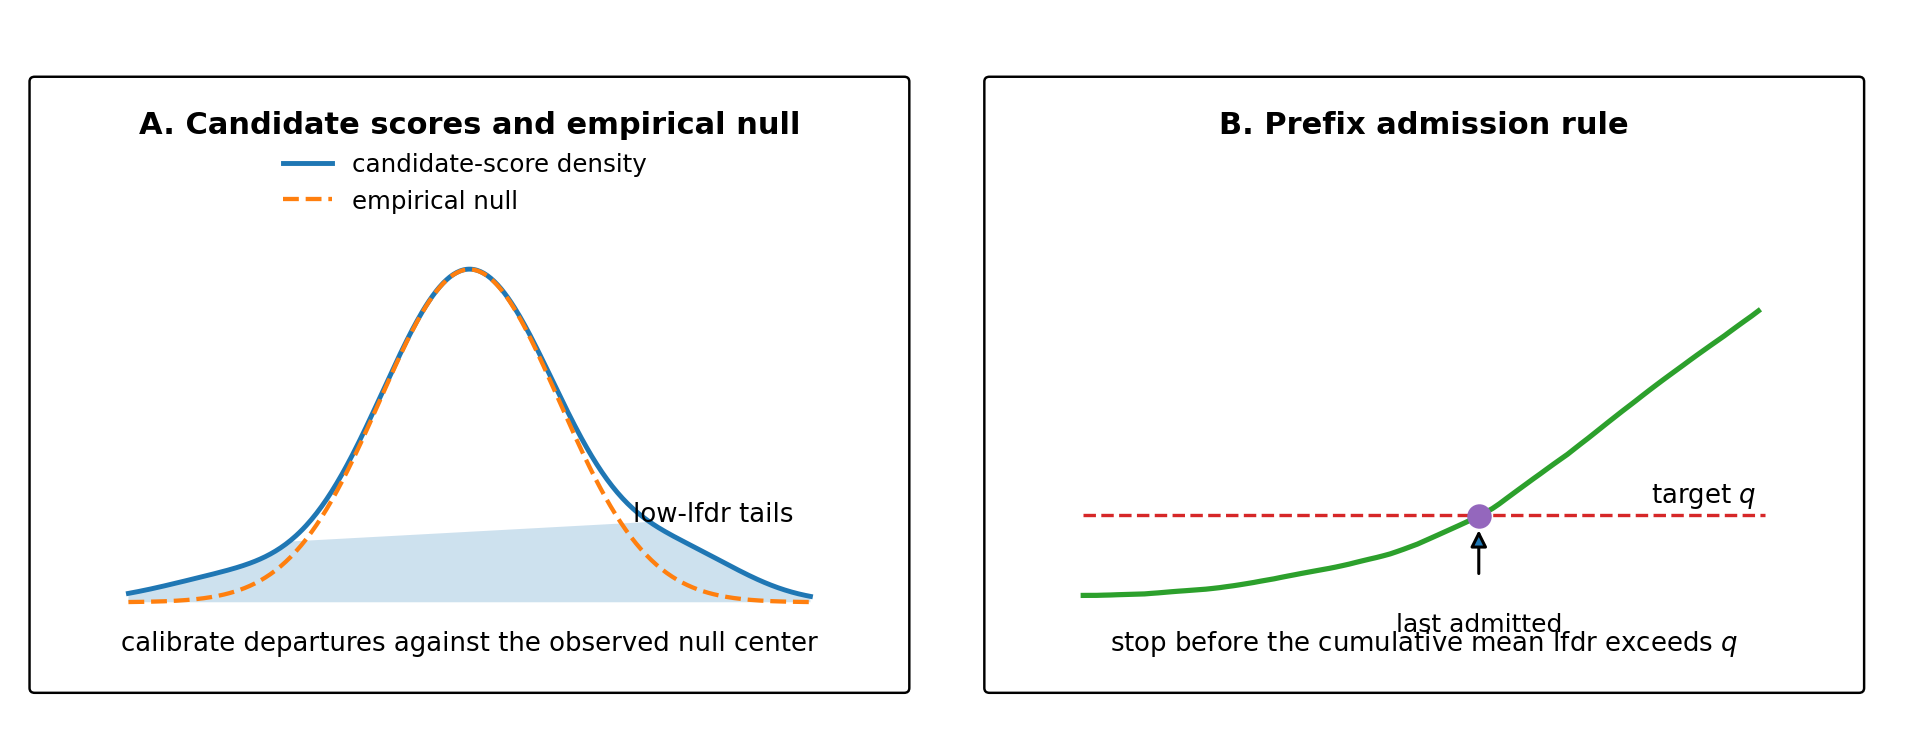
\includegraphics[width=0.98\textwidth]{fig17_lfdr_gate.png}
\caption{A representative local-FDR refinement round. Candidate scores are calibrated against an empirical null; low-lfdr tail candidates are ranked, and the longest prefix whose mean estimated local FDR stays below $q$ is admitted. The figure explains the operational rule; formal qualifications for dependence and adaptive hypothesis generation appear below.}
\label{fig:lfdr-concept}
\end{figure}

\begin{proposition}[Bayes FDR of the prefix rule]\label{prop:fdr}
Under the two-groups model with known $(\pi_0,f_0,f)$,
$\E[\mathrm{FDP}(S)\mid z_{1:M}]=\frac{1}{|S|}\sum_{i\in S}\lfdr(z_i)\le q$ for the
selected set, i.e.\ the rule controls the posterior expected false discovery
proportion at $q$.
\end{proposition}

\emph{Scope of Proposition~\ref{prop:fdr} (downgrade).} Three qualifications
bound what this controls, per an external review we credit. (i) The candidate
$z$'s within a round are positively dependent (adjacent stars share parents
and observations); the expectation argument for Bayes FDR survives dependence,
but the Lindsey estimation of $\hat f$ does not cleanly; histogram counts
are no longer independent Poisson, $\hat f$ has variance the machinery does
not see, and the realized FDP can be substantially more variable than its
expectation. (ii) The floor $\pi_0\ge0.5$ is deliberately conservative and is
wrong mid-refinement when most candidates are true signal, so ``mean lfdr
$\le q$'' then controls a quantity more conservative than the nominal one.
(iii) Most fundamentally, the hypotheses are random: $H_0(v)$ is a functional
of the current mesh, which is a functional of the data through prior rounds
--- a hypothesis-set selection problem outside the fixed-dictionary setting of
Abramovich et al. The honest statement of the proposition is therefore:
\emph{per-round Bayes FDR under the estimated lfdr, conditional on the mesh at
that round}, with whole-run frequentist FDP control an empirical matter, now measured.

\emph{Empirical FDP study (10 seeds per cell).} A gate admission is classified
false when the true hierarchical surplus at the vertex,
$|f(v)-\tfrac12(f(p_0)+f(p_1))|$, is below $\varepsilon$ (primary
$\varepsilon=0.01$ log-odds; results bracketed at $0.005/0.02$);
pre-refinement vertices are excluded, only lfdr-gate admissions count. In
signal regimes the realized FDP is conservative and nearly flat in $q$:
means $0.060/0.062/0.066$ at $q=0.05/0.10/0.25$ on the uniform surface
(admission counts $293/331/465$), $0.068$ under pure white pool noise and
$0.056$ on the chirp at $q=0.10$, with per-seed maxima $\le0.134$; the
conservatism stack ($\pi_0$ floor, dispersion calibration, empirical null)
dominates the nominal target, and at $q=0.05$ the mean mildly exceeds nominal
($0.060$), so control should not be described as tight at the small-$q$ end.
At the \emph{complete null} (zero surface), however, the per-round Bayes
statement visibly fails to deliver whole-run FDP control: seven to eight of
ten seeds admit at least one vertex ($36\pm62$ admissions with frailty
present, $71\pm116$ without, out of a candidate stream in the tens of
thousands), and any admission at the null makes $\mathrm{FDP}=1$, so the
realized FDP is approximately Bernoulli with mean $0.7$--$0.8$ against
$q=0.10$. The absolute false counts are small and the admitted heights tiny
(the no-signal energy floor is unaffected), but the qualitative point stands:
with an estimated null and dependent scores, FDP at or near the complete null
is an excursion event, not a controlled rate; exactly the fragility the
dependence caveat above predicts. Downstream consumers should read the gate
as a conservative discovery filter in signal regimes and as a
small-but-uncontrolled admitter at the null.
\begin{proof}
$\E[\#\{\text{true nulls in }S\}\mid z_{1:M}]=\sum_{i\in S}P(H_{0,i}\mid z_i)
=\sum_{i\in S}\lfdr(z_i)$ by definition of lfdr and (conditional) independence; divide
by $|S|$.
\end{proof}

\begin{remark}[caveats]
Control is exact for the oracle lfdr and one exchangeable batch; in the algorithm
(i) $\lfdr$ is estimated, (ii) rounds are sequential and each round's candidate set
depends on past admissions. The constrained empirical null is conservative for (i);
for (ii) the batch-round structure (test all current candidates, admit, re-converge,
re-test) is the finite-sample analogue of the wavelet-coefficient setting of
\cite{abramovich2006}, and online-FDR procedures (alpha-investing, SAFFRON) are the
fully rigorous alternative if formal sequential control is required.
\end{remark}

\subsection{Coarse scales are not thresholded}
The coarsest hat coefficients of an oscillatory target are near zero (the signal is
nearly orthogonal to the coarse basis), so a gate applied from depth zero can fail to
start: with few candidates and small coarse coefficients, nothing is admitted and the
procedure stops at the initial mesh (observed: 2 faces, entire signal missed).
Following the wavelet-thresholding convention, the mesh is uniformly pre-refined to a
modest face count ($\approx 48$) before gating; the cost is a handful of possibly-null
degrees of freedom, absorbed by the EB prior, against removal of the cold-start failure
mode. For small candidate sets ($M<50$) the Lindsey fit is unstable and a
Benjamini--Hochberg step at level $q$ on two-sided $p$-values replaces it
\cite{bh1995}.

\subsection{Round structure and stopping}
Each round: (1) re-estimate the EB hyperparameters; (2) run coordinate-descent height
sweeps to a tolerance so that candidate residuals are computed against converged
neighbors (unconverged heights contaminate every $z$ in a star); (3) score all
candidates, fit the two-groups model, admit the prefix set; (4) activate admitted
vertices (NVB cascades may add completion vertices, which are structural, not
discoveries). If nothing is admitted, deepen the height convergence and re-test; if the
binomial outer loop is in use, re-expand \eqref{eq:working} at the current fit and
re-test; stop after repeated stalls. The stopping rule is thus intrinsic: refinement
ends when no remaining candidate clears the FDR gate, not when a time or size budget is
exhausted.

\section{Empirical Bayes fitting and shrinkage}\label{sec:eb}

\noindent\emph{Selection bias in $\hat\tau_d^2$ (acknowledged, uncorrected).}
The depth-level moment for $\tau_d^2$ is computed over \emph{admitted}
vertices, whose $\hat\delta_v$ are truncated Gaussians (selected for $|z|$
beyond a data-dependent threshold), not the unshifted Gaussians the moment
identity assumes. Truncation inflates the moment mechanically; the
selected-null contribution alone is $\mathbb{E}[z^2\,|\,\text{selected}]
\approx4$--$9$ at $q=0.10$; so $\hat\tau_d^2$ is biased up by an amount
depending on the threshold and the true slab; the same effect corrected in
the variance-component moments is presently uncorrected here. Two further
honest notes: shrinkage under admitted structure leaves signal-adjacent
residual that biases neighboring candidates' scores in later rounds, a
feedback the theory does not treat; and dropping the $\sum w^2/\sum w$ term
shrinks $\hat\tau^2$, which is conservative against false structure but
anti-conservative for the missed-signal moments downstream, which read the
extra shrinkage as undiscovered energy. The truncated-moment correction is now derived,
verified in isolation, and; instructively; found not to help in the
live loop. For a centered Gaussian $X\sim\mathcal N(0,V)$ selected on
$|X|>a$, $\mathbb E[X^2\mid|X|>a]=V\kappa(a/\sqrt V)$ with
$\kappa(\alpha)=1+\alpha\varphi(\alpha)/(1-\Phi(\alpha))$, so the
selection-consistent depth moment solves
$\chi^2_d=\sum_v\kappa_v(\tau^2)\,(\tau^2+s_v)/s_v-1$ for $\tau^2$
(bisection; reduces to plain DL at $a_v=0$), with $a_v$ recorded at
admission as $c_{\mathrm{round}}$ times the candidate's calibrated standard
error. On synthetic draws with heterogeneous $s$ the naive moment is biased
upward by $+6$ to $+17$ variance units at realistic thresholds; the
mechanism quantified above; while the corrected estimator lands within
$\pm0.09$ of truth, including under $10\%$ null contamination. Deployed
inside the pipeline, however, the correction \emph{worsens} held-out
deviance on two of three seeds and destabilizes the gate on a third, and is
neutral on real data. The cause is localized: the pipeline's moment consumes
already-shrunk (pooled) coefficients, whose $\chi^2$ is deflated relative to
the raw $\hat\delta$ the truncation law describes, so the naive moment's
selection inflation and the shrunk-input deflation partially cancel;
correcting only the former over-corrects, and the smaller $\hat\tau^2$
feeds harder shrinkage and gate feedback. The estimator therefore ships
opt-in (\texttt{DMESH\_TRUNC=1}), the honest theoretical status is that the
prior-estimation moment carries two biases of opposite sign whose partial
cancellation is currently load-bearing, and the principled repair is the
truncated moment applied to \emph{raw admission surpluses}; queued, as it
requires carrying raw coefficients alongside pooled ones.

Admitted surpluses are shrunk under a Gaussian working prior per depth $d$:
$\delta_v\sim N(0,\tau_d^2)$, giving the posterior-mean update
\begin{equation}
\hat h_v=\mu_{\mathrm{lin}}(v)+\frac{\tau_d^2}{\tau_d^2+\sigma^2 s_v}\,
\bigl(\hat\beta_v-\mu_{\mathrm{lin}}(v)\bigr),\qquad s_v=\frac{1}{x^\top Wx}.
\end{equation}
Hyperparameters are estimated by the DerSimonian--Laird moment identity
\cite{dl1986}: for $m$ vertices at depth $d$ with weights $w_v=1/s_v$ and
$Q=\sum_v w_v(\hat\delta_v-\bar\delta_w)^2$,
\begin{equation}\label{eq:dl}
\E Q=(m-1)\sigma^2+\tau_d^2\Bigl(\textstyle\sum_v w_v-\frac{\sum_v w_v^2}{\sum_v w_v}\Bigr)
\quad\Longrightarrow\quad
\hat\tau_d^2=\frac{\bigl[Q-(m-1)\sigma^2\bigr]_+}{\sum_v w_v} ,
\end{equation}
(the implementation drops the $\sum w^2/\sum w$ term, a conservative simplification).
Two selection-aware modifications are essential:

\begin{enumerate}[leftmargin=2em]
\item \emph{Slab, not pooled.} Under a sparse (spike-and-slab) truth, estimating
$\tau_d^2$ over \emph{all} candidates dilutes the slab with nulls and overshrinks every
admitted coefficient. Consistency with the two-groups gate requires estimating
$\tau_d^2$ over \emph{admitted} vertices only: the gate decides existence, the prior
describes the nonnull component. Mild upward selection bias in $\hat\tau^2$ translates
into mild undershrinkage of a set whose false fraction is already bounded by $q$.
\item \emph{A floor, and reversion off support.} An information-starved vertex with
near-zero $x^\top Wx$ takes an effectively unregularized height; its error propagates
into neighbors' residuals, inflates nearby candidate $z$'s, opens the gate into the
damage, and the loop diverges (observed: heights of order $10^{11}$). A shrinkage floor
(equivalently a height sanity clamp resetting to $\mu_{\mathrm{lin}}$) removes the
feedback. Separately, any active vertex whose star contains no data is reverted to the
prior mean $0$: off the data support the deliverable is exactly the internal model.
The prior mean $0$ is the correct one for a \emph{correction} surface; it is what makes
the empty-space behavior auditable.
\end{enumerate}


\section{The admission null: conditional, composite, and permutation formulations}\label{sec:nulls}

The gate of Section~\ref{sec:gate} tests each candidate surplus against a
null distribution, and the choice of that null is a modeling decision with
measurable consequences. Three formulations are now implemented and
characterized. Throughout, the statistic template is
$z_v = (\hat\beta_v - \hat\mu_v)/\mathrm{sd}_v$ feeding the empirical-null
and prefix machinery of Section~\ref{sec:lfdr} unchanged; the formulations
differ only in $\mathrm{sd}_v$ and in its calibration.

\subsection{Conditional null (baseline)}
$\mathrm{sd}_v^2 = (1/X_v + \tfrac14 s_p)\hat\varphi$ with $X_v$ the
star information and $\hat\varphi$ the global Pearson dispersion. This is
the statement that, given the full latent state, $p$ defines pure noise.
The statement is true, and it is the wrong conditioning for the decision:
the vertex never observes the pool state, so under this null pool-level
overdispersion is read as location signal, and structure is admitted at
the wrong address. Under this formulation the empirical-null clamps
($\hat\sigma_0\in[1,1.4]$, $\hat\pi_0\ge0.5$, the depthwise $\tau^2$
floor) are load bearing: removing the $\tau$ floor triggers a shrink,
residual-signal, re-admission spiral (measured on the synthetic
benchmark: mesh $2127\to4697$, held-out $20.7\to27.8$).

\subsection{Composite null (analytic pool-variance form)}
The declared model has two signal layers, surface and pool, and a surface
hypothesis must be tested against the composite null that includes the
pool layer:
\[
\mathrm{sd}_v^2 = \Bigl(\frac{1}{X_v}
 + \sigma^2_{\mathrm{gate}}\,\frac{X^{(2)}_v}{X_v^2}
 + \tfrac14 s_p\Bigr)\hat\varphi,
\qquad X^{(2)}_v = \sum_i \tilde w_i^2 \varphi_v(z_i)^2,
\]
with $\sigma^2_{\mathrm{gate}}$ measured by the per-size instrument
(Section~\ref{sec:physics}). Fit weights are untouched; only admission
requires cross-pool replication. The identification is explicit: pool
noise averages at rate $K_{\mathrm{eff}}^{-1/2}$ with
$K_{\mathrm{eff}} = X_v^2/X^{(2)}_v$ the effective pool count, while a
shared surface shift survives averaging; a star dominated by one pool has
divergent null variance, the continuous form of a minimum-effective-pools
rule. Unreplicated variation is not discarded; it is routed to the pool
layer, which is its correct address. Under this null the clamps were
measured to be compensation for the conditional formulation: the $\pi_0$
floor is inert to the printed digit, the $\sigma_0$ box is near-inert, and
the $\tau$ floor is removable and mildly beneficial.

\subsection{Permutation null (exact conditional-on-effects form)}
The composite null has an assumption-free exact form. Take the null to be:
no spatial signal within the star; residual variation is pool specific.
The pool effects are then nuisance parameters to condition on, not draws
from a law to be modeled: the null distribution of the candidate statistic
is obtained by permuting the observed (residual, variance) pairs across
the star's hat-weight slots and recomputing the statistic. The null then
carries the realized tails, lumps, size structure, and issuer effects with
no mixing-law model at all, and any computation shared by the real and
permuted scores (baselines, fit-state transients) cancels identically.
Measured: on the noise-physics benchmark of Section~\ref{sec:certnull}
this matches the analytic composite gate (6 versus 7 certified-false deep
faces against the baseline's 997) with zero distributional assumptions and
slightly better held-out deviance (16.25 versus 16.8); with weak clean
Gaussian noise it exposes fit-state spatial transients as signal (66 on
the v3 benchmark); on real data it is over-conservative (730 vertices)
because all within-star structure, including genuine sub-face surface, is
priced into the null. It is the correct certification instrument under
realistic noise, and its real-data conservatism is the self-masking cost
of the composite stance made explicit. (Default-gate counts in the table
below are the post-fix values 969/996; an earlier draft carried 886/997
from before the dispersion-denominator correction of
Section~\ref{sec:onelaw}. The composite counts 2/7 are unchanged by that
fix.)

\subsection{The two configurations, precisely}
\begin{center}
\begin{tabular}{p{3.4cm}p{4.6cm}p{5.4cm}}
\toprule
component & conditional (baseline) & composite (principled) \\
\midrule
extra variance is & signal at the surface address & noise for the surface
test; signal for the pool layer \\
clamps & load bearing & measured inert or removable \\
single-pool stars & admissible & not certifiable \\
certified-null v3 deep faces & 969, false with certainty & 2 \\
noise-physics v4 deep faces & 996 & 7 analytic; 6 permutation \\
real held-out deviance/pool & 24.54 & 10.00 \\
marginal NLL per pool & 3.351 & 3.509 \\
in-zone info-weighted deviance & 33.68 & 11.12 \\
\bottomrule
\end{tabular}
\end{center}

The three evaluation metrics disagree by construction
(Section~\ref{sec:metrics}): on a single snapshot the fine-scale structure
is a bundle of genuine sub-face surface and pool-specific variation, and
the two configurations are the two set-identification bounds, the
conditional spending the bundle and the composite pricing it as null. The
measured $(\sigma_{\mathrm{gate}}, q)$ frontier shows the $q$ dial
dominating the $\sigma$ dial: keeping the null fully priced while
admitting more liberally reaches marginal NLL $3.442$ at $51$
certified-false faces, against $3.351$ at $886$ and $3.509$ at $2$.

\section{Residual variation and pool attribution}\label{sec:attribution}

After the gate stops, let $\hat p_i=\sigma(\eta_{0,i}+\hat g(x_i))$,
$\hat w_i=n_i\hat p_i\hat q_i$, and define Pearson residuals
$r_i=(k_i-n_i\hat p_i)/\sqrt{\hat w_i}$. Write the total unmodeled log-odds deviation
as $D_i=\{g(x_i)-\hat g(x_i)\}+u_i$, and decompose its variance as
\[
\Var(D)=\underbrace{\sigma_{\mathrm{sh}}^2}_{\text{spatially coherent miss}}
+\underbrace{\sigma_{\mathrm{id}}^2}_{\text{idiosyncratic }(u,\ \text{frailty, path effects})}.
\]

\begin{figure}[ht]
\centering
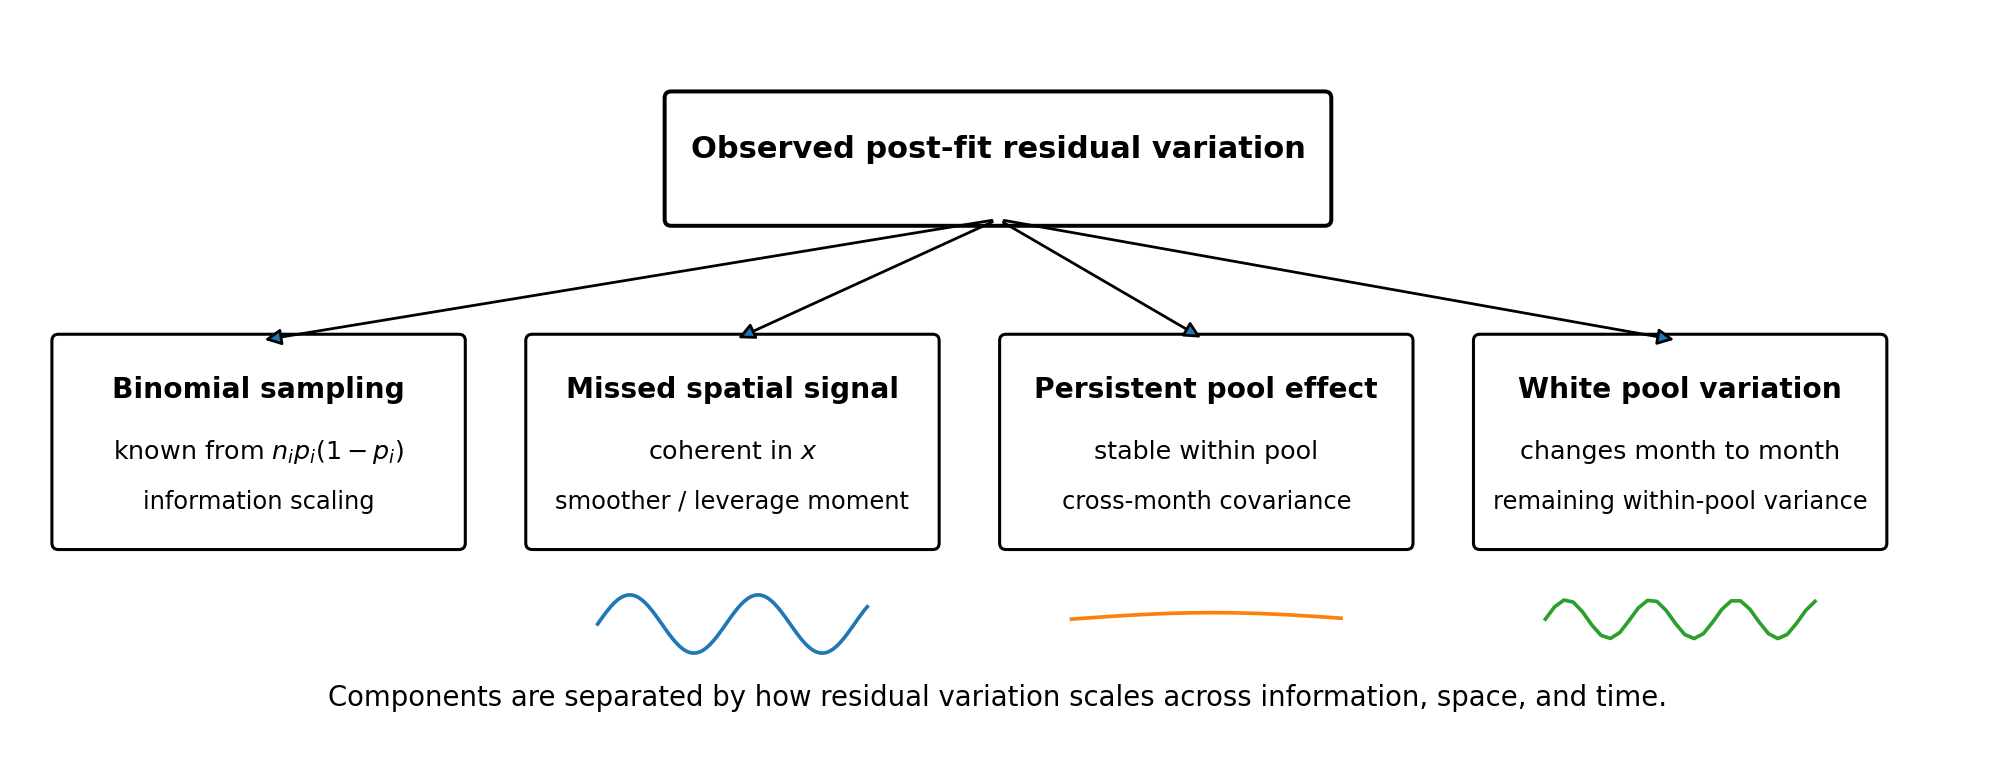
\includegraphics[width=\textwidth]{fig18_residual_attribution.png}
\caption{Conceptual map of the post-fit attribution layer. Binomial variation is known from exposure and fitted probability; coherent residual structure is potentially recoverable by a richer spatial fit; repeated observations identify persistent and white pool components through their different temporal behavior.}
\label{fig:attribution-concept}
\end{figure}

\subsection{Total moment}
Start from the exact binomial decomposition, valid for any $D_i$: with true
$p_i=\sigma(\logit\hat p_i+D_i)$,
\[
\E(k_i-n_i\hat p_i)^2=n_ip_iq_i+n_i^2(p_i-\hat p_i)^2 .
\]
Expanding both terms at $\hat p_i$ (delta method; $dp/d\eta=pq$,
$d(pq)/d\eta=(1-2p)pq$) yields the per-observation identity that drives all the
estimators of this section.

\begin{proposition}[delta-method identity, binomial]\label{prop:total}
\begin{equation}\label{eq:deltaid}
\E[r_i^2]-1
\;=\;
\underbrace{\hat w_i\,D_i^2}_{\text{energy}}
\;+\;
\underbrace{(1-2\hat p_i)\,D_i}_{\text{leakage}}
\;+\;O\!\bigl(D_i^2\bigr)\ \text{terms not scaled by }\hat w_i .
\end{equation}
Consequently, if the leakage term is negligible (see below), with $\mathrm{edf}$ the
effective degrees of freedom of the fit,
\begin{equation}\label{eq:totalmoment}
\widehat{\Var(D)}_{\mathrm{tot}}
=\frac{\sum_i r_i^2-(N-\mathrm{edf})}{\sum_i \hat w_i}
\end{equation}
estimates the $\hat w$-weighted energy $\E_{\hat w}[D^2]$. The level is estimated
not from \eqref{eq:deltaid} but at first-moment efficiency,
\begin{equation}\label{eq:level}
\hat L=\frac{\sum_i\sqrt{\hat w_i}\,r_i}{\sum_i\hat w_i},
\qquad \mathrm{se}(\hat L)\approx\Bigl(\textstyle\sum_i\hat w_i\Bigr)^{-1/2},
\end{equation}
and the energy moment is corrected by
$\hat L\cdot\sum_i(1-2\hat p_i)/\sum_i\hat w_i$ when $\hat L$ is materially nonzero.
\end{proposition}

\emph{Estimand caveat.} The identity identifies a $\hat w$-weighted energy.
The gate refines where information lives, so the residual miss $D^2$
concentrates where $\hat w$ is small; $\hat w$ and $D^2$ are negatively
correlated by construction and the weighted energy understates the unweighted
energy of the miss. Feeding the resulting $\hat\sigma^2$ into the DL weights
as a homogeneous variance is a modeling substitution the fixed-point argument
does not license; it is adopted for its variance-control behavior, verified
empirically. The neglected $O(D^2)$ terms not scaled by $\hat w$ are also
relatively largest for thin pools near the information floor; again where
the miss lives.

\begin{remark}[score annihilation of the leakage]\label{rem:leakage}
At an exact ML fixed point the leakage vanishes: the score equations state
$\sum_i(k_i-n_i\hat p_i)\varphi_v(x_i)=0$ for every active vertex, and since the hat
functions form a partition of unity, $\sum_v\varphi_v\equiv 1$, summing gives
$\sum_i(k_i-n_i\hat p_i)=0$, i.e.\ $\sum_i\hat w_iD_i\approx 0$ to first order.
Regularization breaks this exactly: EB shrinkage attenuates coefficients, the gate
refuses sub-threshold structure, and the outer IRLS terminates finitely, so a
systematic mean residual survives and contaminates \eqref{eq:totalmoment} when $D$ is
large. The level statistic \eqref{eq:level} is the right instrument for it: estimating a
first moment from $r^2$ (e.g.\ by regressing $r^2-1$ on $(\hat w,1-2\hat p)$) costs
orders of magnitude in efficiency and was found empirically to return pure noise even
with $1-2\hat p$ spanning $\pm0.98$, while \eqref{eq:level} resolved the same
quantity to $\pm 0.001$ log-odds. (That precision assumes independent residuals; within-pool frailty correlation implies a design effect that inflates it, so the quoted se is a lower bound.) In sample, the weighted score of exact ML pins
$\hat L$ at zero, so $\hat L$ measures precisely the level that regularization leaves
uncorrected (a direct gauge of EB-plus-gate absorption; it should shrink as the
fixed-point iteration of Section~\ref{sec:posthoc} converges, and it grew
monotonically as the gate was tightened in the $q$-sweep, as designed). Two regime
notes: with $p$ spread widely, $\sum_i(1-2\hat p_i)\approx 0$ and the leakage
correction self-cancels; at hazard scale ($p\sim1\%$, $1-2\hat p\approx1$) it does
not, and a level of $-0.004$ shifts a post-gate energy of $0.01$ by roughly $20\%$,
which is where the correction earns its keep.
\end{remark}

\begin{remark}[validity boundary]
The first neglected contribution to \eqref{eq:deltaid} is a skewness term of order
$\hat w_i(1-2\hat p_i)\,\E D^3$: with a large negatively skewed miss the moment
under-reads (observed empirically on a deliberately degraded fit). No distributional
assumption on $D$ is made anywhere above, the output is directly in log-odds units
(the units the DL weights and the Gamma prior consume), and the small-to-moderate
miss regime after the gate is exactly where the expansion is sharp.
\end{remark}

The following exact alternative covers the large-$D$ regime at the price of a
distributional assumption and a rate-scale detour; it is retained as a cross-check
rather than as the primary statement.

\begin{proposition}[exact Poisson--lognormal inversion]\label{prop:lognormal}
Suppose $p$ is small, $k\mid D\sim\mathrm{Poisson}(\lambda e^{D})$ with
$D\sim N(0,s)$, and the fit is mean-matched, $\hat\lambda=\lambda\E e^{D}=\lambda
e^{s/2}$. Then, with $r=(k-\hat\lambda)/\sqrt{\hat\lambda}$ and information
$\hat w=\hat\lambda$,
\begin{equation}\label{eq:exact}
m \;\equiv\; \frac{\E[r^2]-1}{\hat w}
\;=\; \frac{\E (k-\hat\lambda)^2-\hat\lambda}{\hat\lambda^{2}}
\;=\; e^{s}-1
\qquad\Longleftrightarrow\qquad
s=\log(1+m).
\end{equation}
\end{proposition}

\emph{Register.} The inversion is exact \emph{under its mean-matching premise}
$\hat\lambda=\lambda e^{s/2}$, which the pipeline's penalized, gated fit does
not satisfy (that is the content of the broken-score-annihilation remark), so
this proposition serves as a cross-check under an idealization rather than a
property of the produced fit.
\begin{proof}[Calculation]
By the conditional variance decomposition,
$\E(k-\hat\lambda)^2=\E[\Var(k\mid D)]+\Var(\E[k\mid D])
=\E[\lambda e^{D}]+\Var(\lambda e^{D})
=\lambda e^{s/2}+\lambda^2\bigl(e^{2s}-e^{s}\bigr)$,
using $\E e^{D}=e^{s/2}$ and $\Var(e^{D})=\E e^{2D}-(\E e^{D})^2=e^{2s}-e^{s}$.
Subtracting $\hat\lambda=\lambda e^{s/2}$ leaves
$\lambda^2(e^{2s}-e^{s})=\hat\lambda^{2}(e^{s}-1)$ since
$\hat\lambda^{2}=\lambda^{2}e^{s}$; dividing by $\hat\lambda^{2}$ gives
\eqref{eq:exact}. The empirical statistic
$(\sum_i r_i^2-(N-\mathrm{edf}))/\sum_i\hat w_i$ is the sample version of $m$, so the
missed variance is recovered as $\hat s=\log(1+\hat m)$.
\end{proof}
Expanding $\log(1+m)=m-\tfrac{m^2}{2}+\dots$ shows Proposition~\ref{prop:total} is the
first-order term; at the development magnitudes ($s\approx0.12$, i.e.\ missed sd
$\approx0.35$ log-odds) the correction is $\sim -8\%$ of $m$ and grows with $s$. In the
intended deployment the gate runs first, $s$ is small, and the delta-method
regression of Proposition~\ref{prop:total} is the recommended estimator; the exact
inversion is a cross-check where its assumptions plausibly hold.

\begin{remark}[post-selection bias and the holdout moment]\label{rem:holdout}
Formula \eqref{eq:totalmoment} takes each fitted degree of freedom to absorb one unit
of noise. Gate-admitted vertices are selected \emph{for} large coefficients: under the
null, $\E[z^2\mid |z|>t]=1+t\phi(t)/\{1-\Phi(t)\}\approx 4$--$9$ for $t\in[2,3]$, so an
adaptively selected fit absorbs several noise units per admitted vertex and
\eqref{eq:totalmoment} is biased \emph{low}, by an amount matching the observed
shortfall ($\approx \mathrm{edf}\times 3/\sum\hat w$) in development. The clean repair
is a holdout moment: evaluate $r$ on data the fit never saw (a temporal holdout in
production); then $\mathrm{edf}=0$, no selection adjustment exists, and
\eqref{eq:exact} applies directly.
\end{remark}


\begin{figure}[h]
\centering
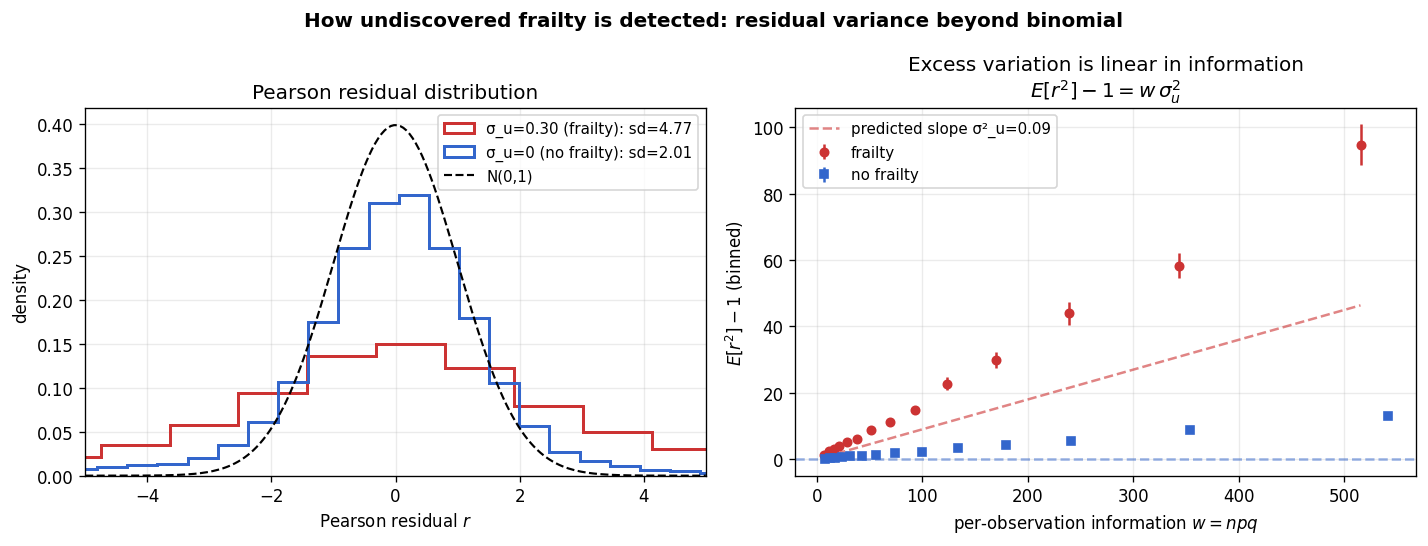
\includegraphics[width=\textwidth]{fig3_residuals.png}
\caption{The estimator's core identity, visualized. Left: Pearson residual distributions with ($\sigma_u=0.30$) and without frailty. Right: binned $\mathbb{E}[r^2]-1$ against per-observation information $w$: with frailty the excess is linear in $w$ with slope $\approx\sigma_u^2=0.09$ (dashed reference); without frailty it is flat near zero, with the mild positive drift at large $w$ reflecting residual surface miss under the density cap. Single seed, $4\times$ data.}
\label{fig:excess}
\end{figure}

\subsection{Shared and idiosyncratic components}
Partition observations into small cells $C$ (side just above the finest mesh scale) and
let $D_i=\Delta_{C(i)}+\varepsilon_i$ with $\Delta_C$ the cell-coherent miss and
$\varepsilon_i$ idiosyncratic across units.

\begin{proposition}[pairwise moment]\label{prop:pair}
For $i\neq j$ in the same cell and different units,
$\E[r_ir_j]=\sqrt{\hat w_i\hat w_j}\,\sigma_{\mathrm{sh}}^2+o(\cdot)$, and
\begin{equation}\label{eq:pair}
\hat\sigma^2_{\mathrm{sh}}
=\frac{\sum_C\bigl[(\sum_{i\in C}r_i)^2-\sum_{i\in C}r_i^2\bigr]
-\text{(same-unit pair terms)}}
{\sum_C\bigl[(\sum_{i\in C}\sqrt{\hat w_i})^2-\sum_{i\in C}\hat w_i\bigr]
-\text{(same-unit pair terms)}}
\end{equation}
is unbiased for the cell-scale-coherent miss; the same construction over within-unit
(same pool, different month) pairs estimates the unit-persistent component
$\sigma_{\mathrm{pool}}^2$ (frailty plus persistent path effects), and
$\hat\sigma^2_{\mathrm{id}}=\widehat{\Var(D)}_{\mathrm{tot}}-\hat\sigma^2_{\mathrm{sh}}$.
\end{proposition}
\begin{proof}[Calculation]
$r_i\approx\sqrt{\hat w_i}\,D_i+\nu_i$ with $\nu$ the standardized binomial noise,
independent across $i$; cross terms vanish and
$\E r_ir_j=\sqrt{\hat w_i\hat w_j}\,\E[\Delta_C^2]$ for distinct units. Summing
$(\sum r)^2-\sum r^2=\sum_{i\neq j}r_ir_j$ over cells and normalizing by the analogous
weight sums gives \eqref{eq:pair}.
\end{proof}

\begin{remark}[the two estimands]\label{rem:estimands}
The pairwise family (and the equivalent variogram nugget-difference estimator) is blind
to miss that is incoherent at cell scale. After a \emph{successful} fit, the remaining
error is P1 interpolation truncation, which oscillates within faces and averages out at
cell scale; the pairwise estimator then correctly reads $\approx 0$ while the total
moment reads the truncation energy. The two are therefore not competitors for one
estimand: the total moment measures everything missed; the pairwise moment measures the
\emph{findable} part (recoverable by further refinement or data); their difference is
resolution-limited truncation plus idiosyncratic variance. In the Monte Carlo
comparison on cosine data with cohort geometry, the total moment had bias $-0.011$,
RMSE $0.038$; cross-validation was unbiased at triple the RMSE; the pairwise and
nugget estimators tracked truth when the fit had failed and read near zero when it had
succeeded, exactly as the estimand analysis predicts.
\end{remark}

\subsection{The report}
The deliverable diagnostic after the gate stops is:
$\hat\sigma_u^2$ from the leverage-corrected pool moment (REML-like in the balanced limit; Paule--Mandel-type moments and REML diverge under weight heterogeneity, which is precisely our regime)
(Section~\ref{sec:doubledip}); the total energy from the $(\hat w,\,1-2\hat p)$
regression of Proposition~\ref{prop:total}, post-hoc centered with its trace or
bootstrap correction; the findable component as total minus idiosyncratic,
cross-checked by the pairwise moment. A holdout evaluation remains available as
insurance, though at production sample sizes the selection absorption it guards
against was measured to be negligible and is in any case covered by the bootstrap
correction.
Interpretation: findable $\Rightarrow$ refine or add data; idiosyncratic
$\Rightarrow$ the missing structure is not in these coordinates (burnout state, pool
frailty), pursue it with an additional state variable or unit-level expression, not
with more triangles. Paired with Proposition~\ref{prop:fdr}, the procedure carries a
two-sided internal accounting, with the FDR side read under the conditional-on-mesh scope of the remark following Proposition~\ref{prop:fdr} and the conditioning table of Section~\ref{sec:conditionality}: at most $q$ of the admitted structure is false in the per-round Bayes sense, and the
undiscovered remainder is measured and attributed. The idiosyncratic component is not
discarded: Section~\ref{sec:posthoc} converts it, pool by pool, into shrunken
posterior attributions.


\subsection{Credibility-weighted pool attribution and the variance fixed point}\label{sec:posthoc}

After the surface is fitted and the variance components are measured, each pool's
realized error admits a posterior attribution into systematic and idiosyncratic parts,
and the attribution changes the estimate for that pool going forward. This section
makes the update exact and identifies the fixed point it satisfies.

\subsection{Credibility form of the posterior}
On the working scale, model observation $i$ of pool $P$ as
$y_i=g(x_i)+u_P+\varepsilon_i$ with $u_P\sim N(0,\sigma_u^2)$ independent of
$\varepsilon_i\sim N(0,1/w_i)$. Given the fitted surface, the residuals
$e_i=y_i-\hat g(x_i)$ over the pool's observed months carry information
$W_P=\sum_{i\in P}w_i$, and the posterior of $u_P$ is Gaussian with
\begin{equation}\label{eq:blup}
\hat u_P=\E[u_P\mid e]
=\frac{W_P}{W_P+1/\sigma_u^2}\;\bar e_P^{\,w},
\qquad
\Var(u_P\mid e)=\frac{1}{W_P+1/\sigma_u^2},
\end{equation}
where $\bar e_P^{\,w}=\sum_{i\in P}w_ie_i/W_P$. This is the BLUP of mixed-model theory
and the B\"uhlmann credibility premium \cite{buhlmann1967,henderson1975}: the observed
pool error is split between idiosyncratic signal and noise in the ratio
$W_P\sigma_u^2:(W_P\sigma_u^2+1)$, so a small pool with two lucky months is shrunk
essentially to zero while a large, persistently deviating pool keeps most of its
residual. The same formula one level up, applied to cross-pool cell means with
$\sigma_{\mathrm{sh}}^2$ in place of $\sigma_u^2$, is the post-hoc revision of the
surface itself; the moment estimators of Section~\ref{sec:attribution} supply exactly the
variance components these weights require.


\begin{figure}[h]
\centering
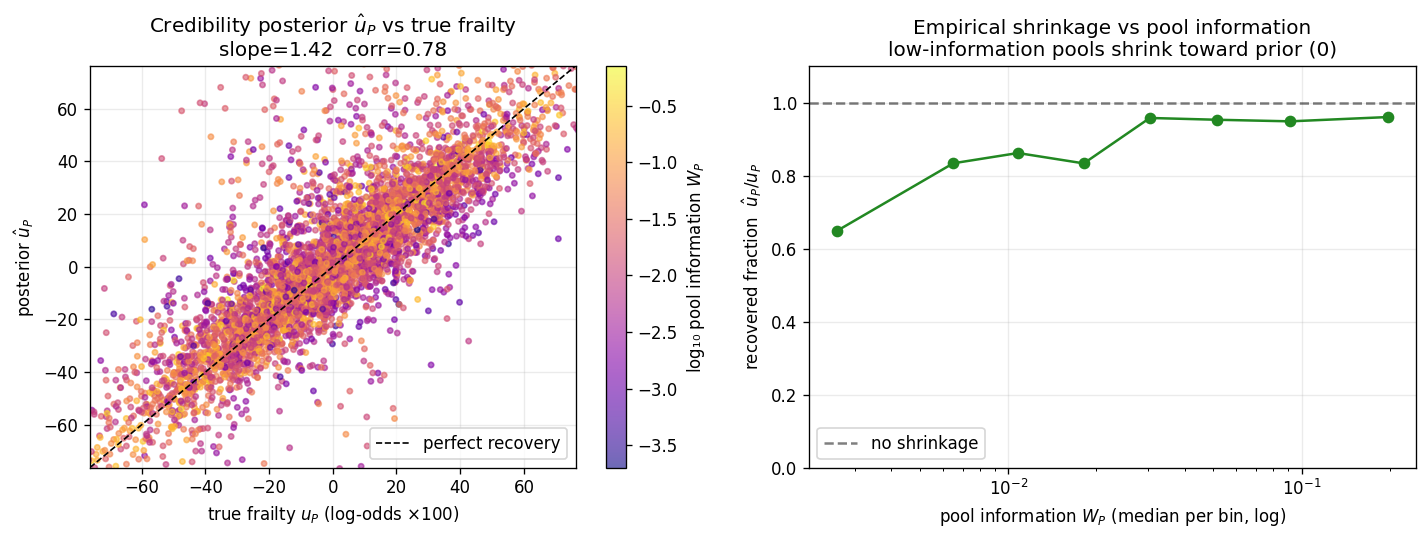
\includegraphics[width=\textwidth]{fig4_blup.png}
\caption{Pool attribution on simulated data ($\sigma_u=0.30$, $4\times$). Left: credibility posterior $\hat u_P$ against true frailty, colored by pool information; corr $0.78$. Right: empirical shrinkage (regression of $\hat u_P$ on $u_P$ within information bins): low-information pools recover $\sim$40--65\% of their frailty and well-measured pools $\sim$95\%, so a thin pool cannot top a ranking on two lucky months. Single seed.}
\label{fig:blup}
\end{figure}

\subsection{The fixed point}
The shrinkage weights in \eqref{eq:blup} require $(\sigma_{\mathrm{sh}}^2,\sigma_u^2)$;
the moment estimators of these components are computed from residuals against the
fitted effects; the fitted effects depend on the weights. The joint solution
$(\hat g,\hat u,\hat\sigma_{\mathrm{sh}}^2,\hat\sigma_u^2)$ is therefore a fixed point,
and it is the familiar one: the stationary point of the (restricted) likelihood of the
mixed model. Alternating (i) posterior effects given variances with (ii) variance
re-estimation given effects resembles an EM alternation, but the moment update is not an M-step and no monotone-ascent guarantee is claimed; with the surface refit and the gate's selection inside the loop, existence and stability of the fixed point are empirical observations in this document,
so the fixed point exists and the iteration is stable under standard conditions.
The pipeline of Sections~\ref{sec:glm}--\ref{sec:overdisp} is a truncated version:
one-step scoring, DL moment \eqref{eq:dl}, DL reweighting \eqref{eq:dlw}, refit is two
Picard sweeps of the same map, and the moment-iterated variant (re-solving the DL
identity at the updated weights until convergence) is the Paule--Mandel estimator
\cite{paule1982}. Running the alternation to convergence is the natural finishing move
of the algorithm and is how the implementation should terminate when the pool layer is
in use.

\subsection{Exact conjugate form on the hazard scale}
The Gaussian working-scale posterior is an approximation; on the hazard scale the
update is exact. Let the pool carry a multiplicative frailty $\theta_P$ on the hazard,
$\theta_P\sim\mathrm{Gamma}(\alpha,\beta)$ with $\E\theta=\alpha/\beta=1$, and let the
month-$t$ events be (small-$p$) Poisson with mean $\theta_P\,\Lambda_{P,t}$, where
$\Lambda_{P,t}=n_{P,t}\hat p_{P,t}$ is the fitted exposure. Then
\begin{equation}\label{eq:gammapost}
\theta_P\ \Big|\ \{k_{P,t}\}\ \sim\
\mathrm{Gamma}\Bigl(\alpha+\textstyle\sum_t k_{P,t},\ \ \beta+\sum_t\Lambda_{P,t}\Bigr),
\qquad
\E[\theta_P\mid\cdot]=\frac{\alpha+\sum_t k_{P,t}}{\beta+\sum_t\Lambda_{P,t}} ,
\end{equation}
closed form in cumulative counts and cumulative fitted exposure, with no logit
approximation; matching $\Var\theta=1/\alpha$ to the measured heterogeneity gives
$\alpha=1/(e^{\sigma_u^2}-1)$ under the lognormal reading of
Proposition~\ref{prop:lognormal}, or $\alpha=1/\sigma_u^2$ to second order. Two
consequences. First, the sufficient statistic $\sum_t\Lambda_{P,t}$ is cumulative
fitted exposure, i.e.\ precisely the burnout state of the population-dynamics
description (Section~\ref{sec:dynamics}): the posterior update of a pool's frailty
\emph{is} the selection functional, one state variable doing double duty for
composition drift and for post-hoc attribution. Second, \eqref{eq:gammapost} exhibits
the credibility structure exactly: the posterior mean is a convex combination of the
prior mean $1$ and the pool's empirical hazard ratio, with weight
$\sum\Lambda/(\beta+\sum\Lambda)$.

\subsection{Dynamics, and what the update is epistemically}
If the pool effect decays, $u_{P,t+1}=\phi\,u_{P,t}+\text{innovation}$, the static
posterior \eqref{eq:blup} is the steady state of a per-pool Kalman filter whose gain is
again a credibility weight; the optimal $h$-step forecast of a pool's error is the
current posterior mean scaled by $\phi^h$, which is the reliability-times-persistence
form measured directly by the frame-attachment panel of Section~\ref{sec:dynamics}.
Finally, the epistemic status of $\hat u_P$ differs from that of the surface: admitted
surface structure is FDR-certified discovery; $\hat u_P$ is a shrunken prediction with
posterior variance \eqref{eq:blup}, licensed by compound estimation (the
hyperparameters are pooled over thousands of pools, so no per-pool selection is
involved) rather than by a test. Ranked by $\hat u_P$, the pool layer is a selection
engine for unit-level expression (specified pools, IO/PO) in which the shrinkage
guarantees that position size in a pool's ``story'' is automatically limited by the
information supporting it.

\subsection{Consistency of the attribution boundary}\label{sec:leverage}

The current exact/quadratic reruns separate two effects that were conflated in the
legacy simulations. First, the five-seed $q$-sweep no longer shows a smooth predictive
U-curve. Among completed fits, held-out surface RMSE decreases from $0.1603$ at $q=0.02$
to $0.1287$ at $q=0.25$ and $0.1016$ at $q=0.50$. The last value is conditional on
success: one of five $q=0.50$ runs failed deterministically through a stage-variance
collapse, as did one of five $q=0.02$ runs. Thus $q=0.25$ is the best robust setting in
this small battery; $q=0.50$ offers lower conditional miss but unacceptable observed
instability. The old statement that large $q$ smoothly overfits noise is therefore
superseded by a fit--stability tradeoff.

Second, fit leverage remains real but is not accurately summarized by a constant
$9\%$ correction. An oracle pairwise moment at the true systematic probability remains
a mechanism-level control, but the current exact/quadratic frailty sweep shows that the
analytic correction is nearly unbiased only at low and moderate frailty and increasingly
under-reads at the top of the tested range. The historical in-sample/holdout bracket
($0.083$ and $0.126$ around a truth of $0.090$) belongs to the legacy pool-moment
implementation; its specialized holdout transformation is not preserved in the current
release scripts and has not been claimed as a current rerun. The structural explanation
is still fit \emph{leverage}: pools-per-vertex-star can remain $O(1)$ as the gate refines,
so the surface absorbs a fraction of each pool's persistent effect. The current evidence
adds a second channel: as frailty rises, robust downweighting and reduced refinement alter
the topology itself, so variance attribution and model selection interact.

\subsubsection*{Analytic leverage correction}
On the working scale after the final expansion, $y=\Phi h+Zu+\varepsilon$ with
$\Phi$ the $N\times V$ hat design, $Z$ the pool indicators,
$u\sim(0,\sigma_u^2 I_P)$, $\varepsilon\sim(0,V)$, $V=\mathrm{diag}(1/w_i)$ the
\emph{binomial} noise variances. The surface is the linear smoother $S=\Phi
A_\Lambda^{-1}\Phi^\top \widetilde W$ with $A_\Lambda=\Phi^\top\widetilde W\Phi+
\Lambda$ and $\widetilde W$ the (DL) fitting weights; residuals $e=(I-S)y$, and if
the admitted surface spans $g$,
\[
e=(I-S)Zu+(I-S)\varepsilon,\qquad M:=I-S .
\]
The pairwise statistic is $T=\sum_P\bigl[(\sum_{i\in P}r_i)^2-\sum_{i\in P}r_i^2\bigr]$
with $r_i=s_ie_i$, $s_i=\sqrt{w_i}$, i.e.\ a sum over same-pool pairs
$\sum_P\sum_{i\neq j\in P}s_is_j\,e_ie_j$. Taking expectations termwise,
\begin{equation}\label{eq:master}
\E[e_ie_j]=\sigma_u^2\,(Mz_{P})_i(Mz_{P})_j+(MVM^\top)_{ij}
\qquad (i,j\in P,\ i\neq j),
\end{equation}
up to cross-pool leak-in terms $(Sz_Q)$, second order and omitted. Hence the exactly
unbiased estimator is
\begin{equation}\label{eq:levcorr}
\hat\sigma^2_{\mathrm{corr}}
=\frac{T-C_{\mathrm{noise}}}{D_{\mathrm{sig}}},\qquad
D_{\mathrm{sig}}=\sum_P\bigl(a_P^2-b_P\bigr),\quad
C_{\mathrm{noise}}=\sum_P\sum_{i\neq j\in P}s_is_j\,(MVM^\top)_{ij},
\end{equation}
where, with the pool-leverage profile
$h_i^{(P)}=\varphi_i^\top A_\Lambda^{-1}c_P$, $c_P=\Phi^\top\widetilde W z_P$,
\[
a_P=\sum_{i\in P}s_i\bigl(1-h_i^{(P)}\bigr),\qquad
b_P=\sum_{i\in P}s_i^2\bigl(1-h_i^{(P)}\bigr)^2 .
\]
The naive estimator replaces $D_{\mathrm{sig}}$ by $\sum_P[(\sum s_i)^2-\sum s_i^2]$
and $C_{\mathrm{noise}}$ by zero, and both replacements bias it \emph{down} through
two distinct channels: the smoother reproduces part of $z_P$, shrinking
$1-h_i^{(P)}$ (the signal channel), and same-pool observations are co-located, so
$S_{ij}>0$ between them and $(I-S)\varepsilon$ acquires negative within-pool
covariance (a noise channel the pure-leverage heuristic misses; this is why the
geometric mean of the in-sample/holdout bracket under-corrects). All ingredients are
quadratic forms in $A_\Lambda^{-1}$: with $\widetilde W=V^{-1}$, $\Lambda=0$ one has
$(MVM^\top)_{ij}=-\varphi_i^\top A^{-1}\varphi_j$ for $i\neq j$; in general
$(MVM^\top)_{ij}=-\varphi_i^\top A_\Lambda^{-1}\varphi_j(\tilde w_jv_j+\tilde
w_iv_i)+\varphi_i^\top A_\Lambda^{-1}BA_\Lambda^{-1}\varphi_j$ with
$B=\Phi^\top\widetilde WV\widetilde W\Phi$. Since each $\varphi_i$ has three
nonzeros, the cost is one factorization of $A_\Lambda$ plus local back-substitutions,
cheaper than a height sweep. To leading order, if $h_i^{(P)}\approx h_P$ over a
pool's observations, $D_{\mathrm{sig}}\approx(1-h_P)^2$ times the naive denominator,
recovering the deflation quoted above. With the EB surplus ridge included,
$\Lambda_{\mathrm{eff}}=C^\top\mathrm{diag}(1/\tau_d^2)C$, where $C$ maps heights to
surpluses ($+1$ at $v$, $-\tfrac12$ at each parent), the correction still improves
calibration. The current five-seed-per-level rerun used
$\sigma_u\in\{0,0.1,\ldots,0.5\}$ and completed all thirty exact/quadratic fits. At
truths $\sigma_u^2=(0.01,0.04,0.09,0.16,0.25)$ the corrected means were
$(0.01008,0.03940,0.08656,0.15166,0.22950)$, corresponding to relative biases
$(+0.8\%,-1.5\%,-3.8\%,-5.2\%,-8.2\%)$. The naive and corrected calibration slopes
through the origin were $0.9132$ and $0.9306$. Thus the trace correction is useful at
every positive frailty level but does not remove bias uniformly. The mean number of gate
admissions also falls from $510$ at the complete null to $96$ at $\sigma_u=0.5$, so the
remaining high-frailty deficit cannot safely be assigned to a fixed-smoother trace term
alone.

A principled replacement estimates the pool variance from likelihood contributions that
were not used to fit the surface. For a surface $\hat g_A$ fit on pool set $A$, define the
held-out pool likelihood
\begin{equation}\label{eq:crossfit-pool-ml}
 L_P(\sigma_u^2;\hat g_A)
 =\int\prod_{i\in P}
 \Pr\!\left\{k_i\mid n_i,\operatorname{logit}^{-1}
 (\eta_{0,i}+\hat g_A(x_i)+u)\right\}
 \phi(u;0,\sigma_u^2)\,du,
\end{equation}
and maximize the sum of $\log L_P$ on held-out pools, adding the symmetric
$A\leftrightarrow B$ term in a two-fold cross-fit. Each integral is one-dimensional and
can be evaluated by adaptive or Gauss--Hermite quadrature. This estimator uses no leverage
multiplier, handles logistic curvature and binomial heteroskedasticity directly, and
breaks the same-data dependence between the fitted surface and the variance score.

The diagnostic sequence is deliberately staged. First estimate $\sigma_u^2$ by marginal
likelihood at the known simulated surface; failure there identifies the pool likelihood or
quadrature. Next compare same-data and cross-fitted marginal likelihood under the current
mesh. Finally hold topology fixed across the frailty sweep, using a rich low-frailty or
$q=0.25$ topology, to determine how much remaining bias comes from early gate termination.
Only if cross-fitting remains biased should candidate gains themselves be replaced by a
frailty-marginal profile that integrates $u_P$ while testing each spatial coefficient.
Robust weights may continue protecting the surface fit, but the variance layer should then
use the full pool likelihood rather than discard large genuine pool effects. Pipeline
bootstrap inversion remains a useful offline check, not the primary estimator and not a
substitute for these identification diagnostics.

\subsection{Post-hoc centering and the double-dip correction}\label{sec:doubledip}

The moments of Section~\ref{sec:attribution} sharpen when centered at the post-hoc
probability $\tilde p_i=\sigma(\eta_{0,i}+\hat g(x_i)+\hat u_{P(i)})$: the
pool-persistent component leaves $D$, the skewness boundary of
Proposition~\ref{prop:total} recedes, and the resulting statistic is the innovation
variance the dynamic pool filter consumes. The cost is double dipping: $\hat u_P$ was
fit to the same counts entering the residuals, and a posterior mean absorbs noise, so
post-hoc Pearson residuals are underdispersed by construction. The deficit, however,
is estimable and correctable rather than avoidable-only.

\emph{Linear layer: trace correction $=$ REML.} The credibility posterior is a
rank-one linear smoother per pool, so under a correct model
\[
\E\Bigl[\sum_i \tilde r_i^{\,2}\Bigr]=N-\sum_P\kappa_P,
\qquad
\kappa_P=\frac{W_P}{W_P+1/\sigma_u^2},
\]
i.e.\ the effective degrees of freedom of the pool layer is the sum of its own
shrinkage factors. Correcting the moment by $\sum_P\kappa_P$, and noting that
$\kappa_P$ depends on $\sigma_u^2$ so that the corrected moment equation is a
one-dimensional monotone fixed point, reproduces the ML-to-REML adjustment
for the variance component in the balanced Gaussian limit: there, and only
there, the double-dip correction coincides with REML.

\emph{Nonlinear layers: bootstrap $=$ covariance penalty.} Where no trace formula
exists (the Gamma posterior is nonlinear in counts; the gate's selection absorption;
the stability clamps), simulate $B$ replicates from the fitted model, push each
through the identical estimator pipeline, and subtract the bootstrap-null mean of the
statistic. This is Efron's covariance-penalty estimate of generalized degrees of
freedom \cite{efron2004pred,ye1998} and corrects double dipping, selection, and
shrinkage uniformly. Agreement between trace and bootstrap on the linear layer is a
standing consistency check; material divergence on real data indicates some component
absorbing more than its linear-theory share.

\emph{Where the trace genuinely fails.} The linearized trace can miss absorption even
when the posterior-mean smoother is linear in the counts, because Pearson-type
statistics are also standardized by an estimated scale: in $(k-\hat\theta\Lambda)^2/
(\hat\theta\Lambda)$ the denominator co-moves with the numerator (a hot pool inflates
both), an additional negative coupling invisible to any mean-smoother trace. Under
Gamma centering with a correct model, the naive excess read $-0.0255$; the linearized
trace removed only $70\%$ of the deficit (residual $-0.0073$, implied df $1489$);
the bootstrap read $-0.0004$ with implied df $2049\pm13$, a $38\%$ df gap
attributable to the standardization coupling. The rule is therefore two lines: on the
Gaussian working-scale credibility layer, trace and bootstrap agree exactly and the
trace is free; wherever the variance function, the Gamma form, or selection touches
the statistic, the bootstrap is the correct answer and the trace-bootstrap gap
measures what the shortcut misses.

\emph{Numerical check} (isolated pool layer, $2{,}000$ pools, histories $3$--$30$
months, $\sigma_u^2=0.09$): the naive post-hoc excess reads $-0.018$ where a correct
model should read $0$; trace-corrected, $-0.00005$; bootstrap-corrected
($B=200$), $+0.00016$, with bootstrap-implied null degrees of freedom $1515$ against
the analytic trace $1498$. The uncorrected variance fixed point converges to
$\hat\sigma_u^2=0.115$ (absorbed noise counted as signal); the REML fixed point to
$0.092$.

\begin{remark}[sequential centering, retained for one purpose]
An alternative that avoids double dipping by construction is prequential centering,
$\hat u_{P,t}$ computed from months before $t$ only. As an \emph{estimator} it is
dominated by the corrected full-information posterior, since it discards data the
correction can account for. It retains one distinct role: one-step-ahead innovations
have conditional mean zero under a correct model, so the leakage coefficient of the
regression in Proposition~\ref{prop:total}, computed on sequentially centered
residuals, is a pure misspecification (innovation-whiteness) test rather than a
regularization diagnostic.
\end{remark}

\subsection{Pool state and its estimators}\label{sec:poolstate}

The pool-state model is
\[
u_{P,t}=a_P+\eta_{P,t},\qquad a_P\sim(0,\sigma_a^2),\qquad
\eta_{P,t}\sim(0,\sigma_w^2)\ \text{i.i.d.\ across months.}
\]
Under it the within-minus-shared lag profile of
Section~\ref{sec:attribution} is flat at $\sigma_a^2$ for every $\ell\ge1$,
so the pairwise moment is exactly unbiased for the persistent component with
no lag attenuation and the leverage correction of
Section~\ref{sec:leverage} applies unchanged. The white component is the structurally hard parameter, for an
identifiable reason: it lives \emph{only} on the diagonal, and the diagonal
is where everything unidentified lands. The persistent component has
off-diagonal structure to be matched on (the flat lag profile); white noise
by definition has none, so every diagonal moment reads
$\sigma_a^2+\sigma_w^2+m(z)^2$ plus selection error, and estimation is a
matter of subtracting the other three with instruments that do not touch
$\sigma_w^2$. The estimator assembles three such pieces. The total comes
from the Paule--Mandel iteration
\[
\sum_i \frac{r_i^2}{1+w_i\sigma}\;=\;N-\operatorname{tr}S(\sigma)
\]
($\operatorname{tr}S$ under working weights plus EB ridge, Hutchinson probes
through the sparse CG; monotone, bisected, under a second). The persistent
part is the leverage-corrected pairwise moment. The miss part is a zero-lag
instrument: co-located (same-face) pairs from \emph{different} pools share
the local miss $m(z_i)m(z_j)$ and nothing else, no frailty across pools and
no white noise across independent draws, so the same-face cross-pool moment
$Z$ estimates the information-weighted local miss second moment up to the
within-face coherence of the $P_1$ interpolation error ($\kappa=15/16$ for
the isotropic bubble). Then
$\hat\sigma_w^2 = \text{PM total} - \hat\sigma_{a,\mathrm{corr}}^2 - Z$.
The identifiability boundary is the zero-lag twin of the earlier ones: miss
varying below the face scale \emph{and} below the monthly trajectory step is
observationally equivalent to white pool noise, on the diagonal and along
trajectories alike, so $Z$ recovers the resolved miss and sub-face amplitude
variation remains inside $\hat\sigma_w^2$ by convention.

\emph{Verification} (uniform surface unless noted; three to five seeds per
cell; truth total $0.09$ split as $\sigma_a^2/\sigma_w^2$). Persistent
component: scale-consistent ($\hat\sigma_{a,\mathrm{corr}}^2 =
0.085/0.090/0.088/0.090$ across $1$--$16\times$ at permanent share $1$;
$0.048/0.045/0.044/0.044$ at share $\tfrac12$), gate-insensitive ($0.0447$
vs.\ $0.0453$ at $q=0.05/0.25$), and falsification-clean (pure white and
no-signal both read $-0.0001\pm.0012$: no manufactured persistence). Its
chirp inflation ($0.117/0.054$) is the attribution semantics of
Section~\ref{sec:attribution} operating as intended. White component
(miss-adjusted, three seeds per cell): $0.050/0.043/0.047$ across
$4/8/16\times$ at the half mix (truth $0.045$; the $16\times$ spread is
$\pm.0003$), $0.092/0.088$ under pure white noise (truth $0.09$),
$0.004/0.003$ in the pure-permanent case, and, decisively, $0.004\pm.004$
on the chirp, where the instrument routes the large multi-scale miss into
$Z=0.019$ rather than into $\hat\sigma_w^2$. The residual error decomposes as follows, dominant
cause first. (i) \emph{Selection gap in the PM trace}, now quantitatively
attributed: the trace treats the gate-selected basis as fixed, and the
double-dip analysis measured the selection surplus at $\approx38\%$ of the
nominal edf; with edf $\approx660$ and the measured PM sensitivity
$\partial\sigma/\partial\mathrm{edf} = 1.9\times10^{-5}$ (from
$\sum_i w_i/(1+w_i\sigma)^2 \approx 5.3\times10^4$ at the half mix), the
predicted bias is $+0.0047$ against the observed $+0.0052$; essentially the
entire systematic error. The definitive measurement is instrumented (split
randomness fixing data locations while resampling outcomes, per-observation
fit dumps) but requires a fixed-point linearization of the working response,
since the IRLS response contains the fit and naive covariance double-counts
it; that measurement, and the edf substitution it licenses, are the queued
repair. A first attempt at the split-randomness measurement was run and
diagnosed rather than trusted: the outcome-only replicate stream redraws
pool frailty $(a_P,u)$ alongside the binomial count, so replicates differ in
their \emph{true} $p_t$, not only in binomial sampling noise: the observed
spread of $\hat p$ across replicates (median $0.023$) exceeds the
pure-binomial expectation at typical pool size (${\approx}0.020$) only
mildly at the median but by an order of magnitude in the upper tail,
consistent with a subset of pools re-drawing frailty. Efron's formula then
divides by the wrong (too-small) variance and the resulting edf is not
usable. The correct instrument needs a three-way split, locations, frailty,
and terminal binomial draw, each independently controlled; the two-way split
here isolates the mechanism but not yet the number. (ii) \emph{$\kappa$ approximation}: $15/16$ is exact for the
isotropic interpolation bubble under uniform within-face density; NVB
anisotropy, lumpy density, and post-shrinkage (rather than interpolation)
miss profiles perturb it in either direction, bounded by the small size of
$Z$ itself. (iii) \emph{Sampling covariance of the pieces}: the PM total and
$Z$ read the same miss realization, so their seed noise partially cancels in
the subtraction (at $8\times$, $\mathrm{sd}(Z)=.021$ exceeds
$\mathrm{sd}(\hat\sigma_w^2)=.011$); the subtraction reduces variance as
well as bias. (iv) \emph{Plug-in $\hat\sigma_a^2$} propagates one-for-one
($\pm.003$). (v) \emph{Cross-leverage deflation} of the residuals enters PM
and $Z$ with the same sign and largely cancels; second order. (vi) The
\emph{sub-face boundary}: miss below the face scale and the monthly step is
inside $\hat\sigma_w^2$ by convention, a bias only relative to a finer
notion of miss than the method defines. $\hat\sigma_w^2$ remains excluded from the DL weights: with the
miss-adjusted estimator it is now eligible, and its inclusion is an
efficiency study, not a repair; the persistent component alone feeds the
weights until that study is run.

\emph{Development record, kept for its two findings.} The naive diagonal
contrast for $\sigma_w^2$, $(\sum r_i^2-(N-\mathrm{edf}))/\sum w_i$ minus
the persistent and shared terms, is inconsistent: seed spread grows to
$\pm.148$ at $16\times$ because the binomial-scale $(N-\mathrm{edf})$
correction mis-accounts overdispersion absorbed by gate-admitted vertices,
an error that scales with mesh size; the PM trace under working weights is
the repair. And with no persistent component the pre-calibration gate
mass-admitted: overdispersed scores exceed the empirical-null
$\sigma_0\le1.4$ box, selection no trace can price; the dispersion
calibration is that repair, at one measured cost (the stricter gate leaves
slightly more zero-lag miss for the PM total to include: half-mix
$\hat\sigma_w^2$ $0.060$ vs.\ $0.050$ at $16\times$).

Figure~\ref{fig:finalmesh} shows the final-state meshes across regimes; the
center panel is the calibration made visible: pure white pool noise grows
the mesh only $\sim$15\% over the persistent reference (804 vs.\ 700
vertices). A closing battery (three seeds each) confirms no regressions:
chirp attribution $0.117/0.054$, gate insensitivity $0.0448/0.0461$, scale
consistency $0.0476\to0.0452$.

\begin{figure}[h]
\centering
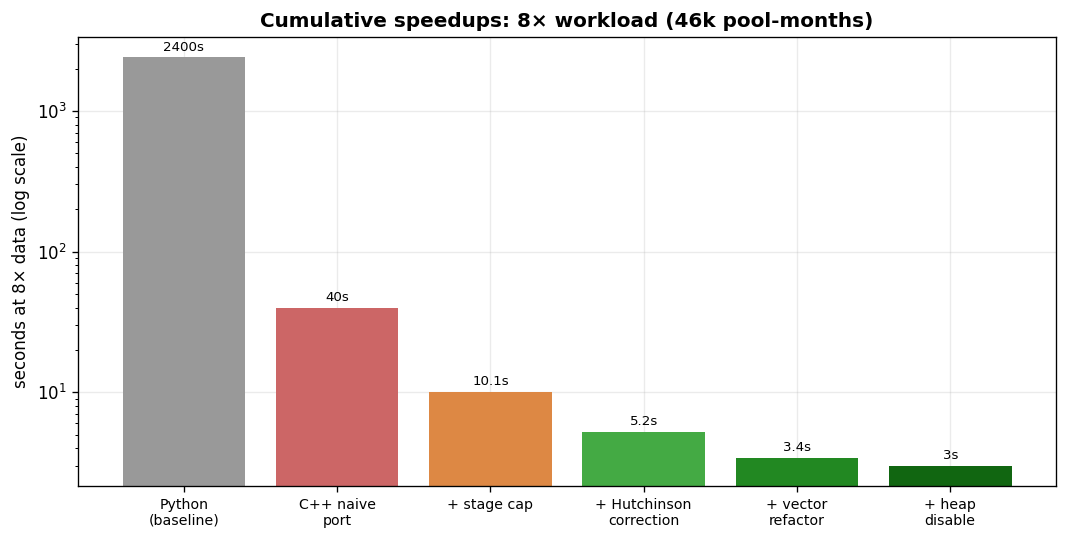
\includegraphics[width=\textwidth]{fig13_final_meshes.png}
\caption{Final-state meshes ($4\times$ data, seed 7, data region). Left:
uniform cosine, pure persistent frailty (1{,}315 faces, 700 vertices).
Center: same target, pure white pool noise (1{,}528 faces, 804 vertices):
the dispersion-calibrated gate admits only $\sim$15\% more vertices where
the uncalibrated gate mass-admitted. Right: chirp (1{,}807 faces, 925
vertices), triangle size tracking local wavelength up the WAC axis.}
\label{fig:finalmesh}
\end{figure}

Autoregressive interpolation ($u_{P,t}=a_P+v_{P,t}$, AR(1) $v$) was
prototyped and shelved: the lag-profile fit identifies the total robustly,
but the permanent/decaying split is horizon-limited (persistence with
$(1-\phi)L\lesssim1$ over an $L$-lag panel is observationally equivalent to
permanence, $L\approx25$--$30$ under cohort attrition) and the lag-zero
extrapolation destabilizes at both $\phi$ extremes. White-plus-permanent
keeps every downstream consumer simple: the credibility posterior is the
static BLUP on $a_P$ with white noise folded into the observation variance.

\section{Theoretical scope and inferential status}\label{sec:scope}

The components of the procedure have different formal status. The table below is intended to keep
those distinctions visible without interrupting every derivation.

\begin{center}
\small
\begin{tabularx}{\textwidth}{p{0.18\textwidth}p{0.18\textwidth}X p{0.20\textwidth}}
\toprule
Component & Status & Main qualification & Principal check \\
\midrule
Candidate score & Local asymptotic approximation & Working WLS neighborhood must be sufficiently converged & Complete-null and score-calibration simulations \\
Local-FDR gate & Conditional empirical-Bayes FDR rule & The candidate family is adaptively generated & Realized FDP and $q$ sweeps \\
EB shrinkage & Working hierarchical model & Depth prior is estimated after selection & Held-out deviance and EB ablations \\
Residual moments & Delta-method and moment identities & Unresolved spatial signal can contaminate pool variance & No-frailty, chirp, and scale experiments \\
WACLS exposure & Exact first-two-moment match & Common conditional event probability within a pool & Heterogeneous-loan-size calibration \\
Pool attribution & Mixed-model/credibility approximation & Requires repeated observations and a stable surface & Persistent-versus-white experiments \\
\bottomrule
\end{tabularx}
\end{center}

\subsection{Conditionality and dataset reuse}\label{sec:conditionality}

One dataset is reused across the empirical null, the gate, the EB
hyperparameters, the variance components, and the pool posteriors. This
section makes the reuse explicit: the estimation order, what each output is
conditional on, where the same data enters an output twice, and what (if
anything) prices that reuse. The intent is that every downstream claim in
this document can be read with its conditioning set attached.

\medskip
\noindent\textbf{Estimation order.} Within a stage: (1) working weights from
the previous stage's $\hat\sigma_a^2$ (binomial at stage 0); (2) refinement
rounds, each comprising candidate scores, the dispersion calibration
$\hat\varphi$, the Lindsey empirical null $(\hat f,\hat\sigma_0,\hat\pi_0)$,
the lfdr prefix gate, EB re-estimation of $\hat\tau_d^2$ over admitted
vertices, and shrunk height updates, with IRLS re-expansion every third round;
(3) on the final mesh, the moment estimators $\hat\sigma_a^2$ (pairwise,
leverage-corrected), the PM total, energy and level, and the BLUP pool
posteriors. Three stages iterate the weights toward their fixed point.

\medskip
\begin{center}
\small
\begin{tabular}{@{}p{2.6cm}p{4.2cm}p{4.6cm}p{3.2cm}@{}}
\toprule
\textbf{Output} & \textbf{Conditional on} & \textbf{Reuse / unpriced selection} & \textbf{Priced by} \\
\midrule
Gate admissions (mesh) & mesh at round; $\hat f,\hat\sigma_0,\hat\pi_0$;
$\hat\varphi$; weights (hence prior-stage $\hat\sigma_a^2$); $\hat\tau_d^2$
via shrunk residuals & candidate $z$'s built from the same residuals that
estimated the null and $\hat\varphi$; hypothesis set itself data-dependent &
empirical null re-centering (partial); FDP measured across seeds: $\approx0.06$ in signal regimes, uncontrolled excursions at the complete null (remark after Proposition~\ref{prop:fdr}) \\
\addlinespace
$\hat\varphi$ (dispersion) & current fit; edf $=$ active-vertex count &
edf produced by the gate that $\hat\varphi$ calibrates; selection absorbs
$>1$ noise unit per admitted vertex & unpriced; direction conservative for
admission \\
\addlinespace
$\hat\tau_d^2$ (EB prior) & admitted set at depth $d$; current weights &
moment over \emph{selected} (truncated) coefficients; feedback into next
round's scores & unpriced (correction queued) \\
\addlinespace
$\hat\sigma_a^2$ & final $\hat g$; mesh; weights & residuals fitted on the
same data; own-pool leverage & analytic correction (\S9.5--9.6), oracle-validated;
plug-in in $\hat\tau,\tilde w$ covered by bootstrap \\
\addlinespace
PM total, $\hat\sigma_w^2$ & final $\hat g$; trace under working weights
$+$ EB ridge; $\hat\sigma_a^2$ subtraction & trace treats the gate-selected
basis as fixed (Efron gap); zero-lag miss inseparable & unpriced; stated as
diagnostic with known confound \\
\addlinespace
Energy, level & final $\hat g$; vertex-count edf & same residuals as all
above; edf at binomial scale & identity checks internal only \\
\addlinespace
BLUP $\hat u_P$ & final $\hat g$; $\hat\sigma_a^2$; weights & pool's own
data in both $\hat g$ and its posterior & shrinkage is the mitigation, not
a correction \\
\addlinespace
Held-out deviance (\texttt{SPLIT}) & even-indexed fit only & none w.r.t.\
surface, gate, and EB (odd pools carry $\approx0$ fit weight) & out-of-sample
by construction \\
\bottomrule
\end{tabular}
\end{center}

\medskip
\noindent\textbf{Reading.} Three circularities are structural: the
weights--$\hat\sigma_a^2$ loop (iterated as the three-stage fixed point,
convergence empirical), the $\hat\varphi$--edf loop (the calibration relies
on the accounting that Remark on selection says is biased; the two errors
push in opposite directions and which wins is regime-dependent), and the
null--gate loop (the null is estimated from the same scores it judges).
Accordingly: FDR statements are per-round Bayes, conditional on the mesh;
$\hat\tau_d^2$ and $\hat\sigma_w^2$ are point estimates with acknowledged
selection bias; $\hat\sigma_a^2$ is the one output with an
oracle-validated correction for its principal reuse channel; and the
held-out deviance is the only fully out-of-sample quantity produced by the
pipeline. Claims elsewhere in the document should be read against this
table.

\section{Evaluation metrics and the reporting standard}\label{sec:metrics}

Held-out deviance per pool is verified correct and tail-fragile: the top
$100$ of $60{,}297$ held-out pools carry $16.5$ of the baseline's $24.54$,
and the $19$ mega pools average $9{,}475$ each (against ${\approx}1{,}359$,
near their irreducible floor, under the composite gate). It is a
$19$-pool story wearing a $60{,}000$-pool denominator. The headline metric
is therefore the held-out marginal likelihood with the pool effect
integrated out (Gauss--Hermite at fixed $\sigma_{\mathrm{pool}}$), which
scores each pool at $n_{\mathrm{eff}}$ and bounds its influence. The
outlier tail itself was forensically informative: $95\%$ same-sign errors
traced to the within-cell size effect above, an omitted formation
covariate rather than noise. The reporting standard is the triple
(marginal NLL, information-weighted deviance in the differential-refinement
zones, certified-null deep count); a configuration dominates only if it
wins all three, no single-snapshot configuration does, and the panel or
loan-level success criterion is exactly to match the conditional bound on
the first while matching the composite bound on the second and third.


\section{August 5 audit: exact-solver default, one-law gate, and the converged SMM law}\label{sec:aug5}

Status header for the whole section: every number below is a measurement from
the August 5 session on the June 2026 SMM design (33{,}740 pools with
$n_0\ge 25$, 9.59M loans, pooled monthly rate $0.852\%$), run on the
2026-08-01 release source rebuilt from scratch, with an external split-mask
replay patch (\texttt{DMESH\_SPLIT\_MASK}) added to \texttt{dataset.cpp} so
the ten stratified Monte Carlo masks from the August 5 external diagnostic
could be reused bit-identically. Held-out deviance per pool is reported for
comparability with that diagnostic; the held-out mixture NLL under the shared
law remains the approved headline instrument.

\subsection{The external diagnostic and its resolution}

An independently produced diagnostic (August 5) refit ten train/test splits
from scratch and found the mesh competitive on ordinary splits but subject to
local eruptions on a minority: fitted probabilities pinned at 0 or 1 in
deeply refined stars with contradictory pools and sub-unit effective support
(worst case: a held-out $0/376$ pool fitted at $0.999943$; the dominant
vertex drew $88.1\%$ of its reconstructed local information from one training
pool). The diagnosed mechanism matches the July forensics verbatim: saturated
pools lose IRLS Hessian weight, so opposition exits the curvature and the
shrinkage self-confirms.

Resolution: the diagnostic's harness never enabled
\texttt{DMESH\_PL\_SOLVER}. Rerunning the identical ten masks with the
phase-A exact solver enabled (and the final retirement audit re-enabled)
removes the failure class entirely: maximum held-out probability $0.188$
across all ten splits, worst single-pool deviance $1{,}443$ versus
$13{,}335$, the canary pool fixed from $0.9998$ to $0.063$, and mean
held-out deviance $1.175$ versus $1.243$ for the per-split tensor GAM,
winning on all ten splits on the diagnostic's own instrument. The GAM's
apparent mean advantage in the external report was purely tail control of a
solver path this release does not need to run.

Consequence adopted: \textbf{the exact solver is the default}; the quadratic
path survives only as a legacy reference. Every subsequent number in this
section is under \texttt{DMESH\_PL\_SOLVER=1}.

\subsection{Null-size measurement and two generator forensics}

True-null batteries on the real SMM geometry (constant logit at the pooled
rate; ten seeds per cell) measured the realized size of the admission
machinery directly, since any admission on a flat surface is false.

\emph{Clean null} (pure binomial): the Lindsey gate under the exact solver
shuts, $0.1$ admissions per run; the legacy quadratic path erupts on pure
noise in 2 of 10 seeds (347 and 447 admissions).

\emph{Heavy-tail nulls} produced two false alarms that forensics traced to
the test constructions, not the gate:

\begin{enumerate}[leftmargin=2em,itemsep=2pt]
\item \textbf{Jensen contamination.} Stratified i.i.d.\ logit mixing shifts
the marginal event rate by $\mathrm{Var}(u)/2$-order amounts that differ by
stratum ($+0.077/+0.135/+0.014/+0.002$ logits under the converged law), and
because exposure strata map onto $(\mathrm{WALA},\mathrm{WAC})$ geography,
the ``null'' datasets carried a genuine $\approx 0.1$-logit spatial signal.
Seed-dependent admissions of small graded heights were power against that
artifact, not size error. Corrected generators recenter each stratum's base
so the marginal rate is flat.
\item \textbf{Central matching versus composite pricing.} On a clean null
the one-law gate (below) prices pool variance absent from the data; the
$z$ bulk deflates (fitted empirical-null sd $0.37$--$0.58$), central
matching adapts the null down to the deflated bulk, and the least-deflated
candidates --- the mega band, whose stratum variance is near zero --- are
flagged as relative outliers. Fix: floor the fitted empirical-null sd at 1
whenever one-law pricing is active (\texttt{DMESH\_SIGMA0\_MIN=1.0}); the
floor is inert on real data, where the priced variance is present, and
removes the anomaly seeds exactly.
\end{enumerate}

\subsection{Pooled-permutation gate: the audit does not transfer to the SMM regime}

The experimental pooled-permutation BH branch (Section on the permutation
audit) was retested under the exact solver on the SMM design. Its
conclusions fail in both directions there. Null control: 85 admissions per
run at the audited operating point ($K_{\mathrm{eff}}\ge 4$, $q{=}.15$)
against the measured SMM law, and 53 per run even against the audit's own
milder $90/10$ mixture --- versus the audit's zero on the April design.
The April benchmark ran at baseline probability $0.78$ with fat counts;
the SMM regime is $p\approx 0.85\%$ with a floor-exposure design, where the
three-moment permutation standardization degrades (mechanism hypothesis;
counts measured). Real data: mean held-out deviance $1.264$, worse than the
Lindsey exact-solver baseline on all ten splits. The rejection recorded in
the August 1 audit therefore stands and strengthens; the branch remains
research-only, and the double-saddlepoint tail computation is the natural
repair if it is revisited, being exact in the sparse-count regime.

\subsection{One-law gate and the converged SMM pool law}

The composite $\sigma^2(n)$-plus-shape admission null
(\texttt{DMESH\_ONELAW}; the continuous form of a minimum-effective-pools
gate) was activated and the joint surface--law fixed point was rerun under
the exact solver with damping $0.5$. It converges cleanly --- held-out
deviance $1.216\pm 0.002$ on the reference split, law drift under $2\%$ per
iteration, no trace of the oscillation the external diagnostic reported ---
confirming the eruption was the oscillation's fuel.

\textbf{Converged SMM pool-effect law} (per stratum: $\pi_{\mathrm{heavy}}$,
tail variance, total variance; excess kurtosis):
\[
(<128):\;(3.7\%,\,1.36,\,0.143;\ 8.5)\qquad
(128\text{--}512):\;(7.6\%,\,1.62,\,0.242;\ 8.1)
\]
\[
(512\text{--}4096):\;(1.8\%,\,0.31,\,0.029;\ 5.4)\qquad
(4096+):\;(1.0\%,\,0.004,\,0.004;\ 0.0)
\]
The earlier law estimated inside the oscillating fixed point is retracted as
a law estimate: its totals were inflated $4$--$17\times$ and its tail
variances $10$--$50\times$ by surface-error absorption. Nulls generated from
the inflated law had produced apparent false-admission rates of order $10^2$
per run; against flat-marginal nulls from the converged law, the realized
sizes at $q{=}.10$ are: \textbf{one-law gate with the sd floor, $0.2$--$0.3$
false admissions per run (9 of 10 seeds exactly zero)}; naked Lindsey,
$11.0$ per run with a fat seed tail (maximum 88, chance heavy clusters it
has no pool-variance term to refuse).

\subsection{Instrument calibration}

Measured against known truth on the corrected generators: the clean-null
falsification of the moment ledger is exact (energy and PM total read zero
to four decimals). Under the converged heavy law the moment instruments run
hot: PM total $0.504$ against an injected pool-weighted $0.145$, energy
$0.121$ against $0$; and against the retracted inflated law they saturate
outright (PM pinned at its cap on all seeds). The mixture-EM law estimate is
therefore the primary variance instrument on this design; the PM total is
usable with the null-derived $\approx 3.5\times$ correction, which
reconciles it with the EM law on real data ($0.603/3.5\approx 0.17$ versus
$0.145$). The pairwise $\sigma_a^2$ instrument proper is structurally
unmeasurable on a single snapshot (one row per pool); true persistence
requires the two-month panel.

\subsection{Fitting-weight ablation and a rejected refinement}

Law-tempered fitting weights (\texttt{DMESH\_LAW\_WEIGHTS}), inherited from
a configuration whose gate did not price pool variance, double-charge pool
noise when combined with the one-law gate: an ablation on the one regressing
split isolates them exactly (with weights $1.249$, without $1.085$,
independent of the sd floor), the damage being $\sim$34 refused ridge
admissions whose coarse triangles bleed a fast ridge onto slow mega
neighbors. They are removed from the recommended configuration.

A two-currency variant was implemented and tested
(\texttt{DMESH\_LAW\_WEIGHTS\_FINAL}: binomial-information currency through
adaptation and admission, GLS law temper applied only to the
frozen-topology final height solve). Measured effect: $+0.0044$ raw
deviance, $-0.0004$ held-out mixture NLL, gains concentrated on the
flip-prone splits. \textbf{Not adopted}: the gain does not justify the added
configuration surface. The flag ships as an experimental option only.

\subsection{Recommended configuration and measured properties}

\begin{center}
\texttt{DMESH\_PL\_SOLVER=1}\quad
\texttt{DMESH\_ONELAW=}$\langle$converged law$\rangle$\quad
\texttt{DMESH\_SIGMA0\_MIN=1.0}
\end{center}
with binomial-information weights throughout and no law-tempered fitting
weights. Measured on the ten external masks: mean held-out deviance
$1.189$ ($\approx$148 admissions per split; beats the tensor GAM on 8 of
10 splits; gives up $0.015$ to the naked gate as the price of the
certification), held-out mixture NLL $0.930$, and $0.2$--$0.3$ false
admissions per run on the honest null battery.

\subsection{Star-level diagnostics}\label{sec:aug5-stars}

The session standardized an annotated star plot as the unit of audit: pools
as markers (circles training, squares held out, area proportional to
exposure), colored by the posterior mean pool effect $\hat u$ under the
shared law given the fitted surface; vertices as diamonds (yellow free,
green conformity) labeled with human-scale height (log-odds and monthly
probability), surplus $\Delta$ over parent interpolation, effective pool
support $K_{\mathrm{eff}}=(\sum \omega b)^2/\sum \omega^2 b^2$, and the
trust ratio $T = X^{\top}X/(X^{\top}X+\lambda)$. Three reference frames
under the recommended configuration: a healthy high-support star
(Figure~\ref{fig:star-high-keff}), the gate's worst held-out pool
(Figure~\ref{fig:star-worst-pool}), and a sparse region
(Figure~\ref{fig:star-sparse}):

\begin{figure}[H]
\centering
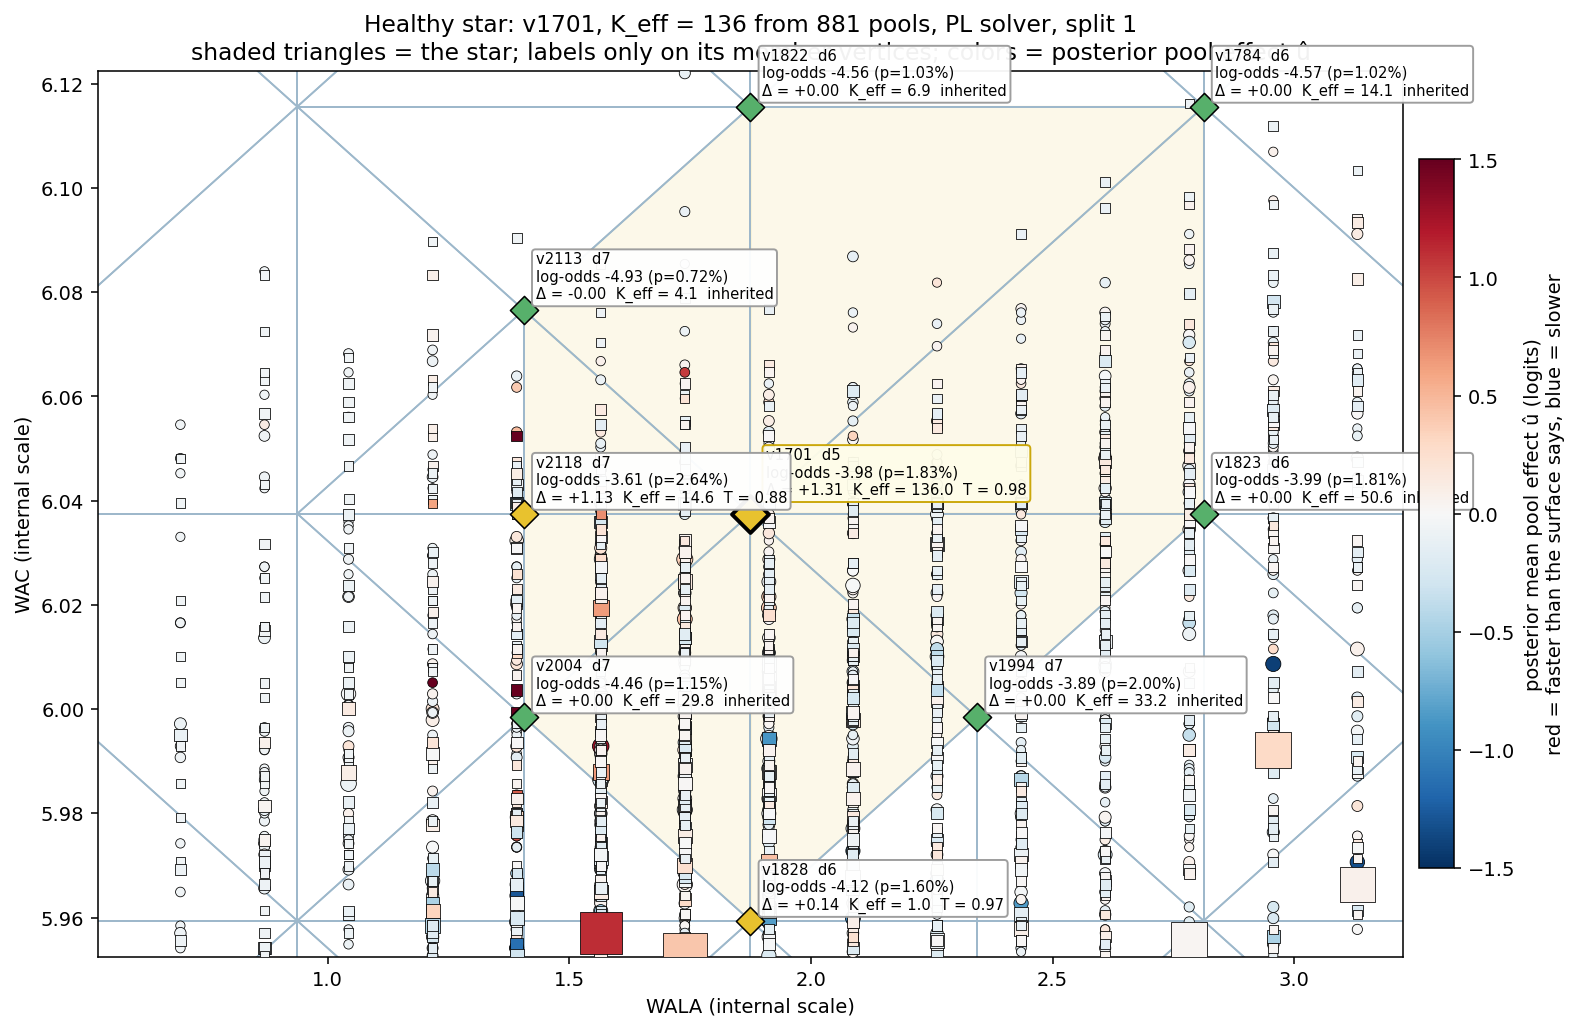
\includegraphics[width=0.95\linewidth]{split1_star_high_keff.png}
\caption{A healthy star: the highest-$K_{\mathrm{eff}}$ free coefficient in
the split-1 fit ($K_{\mathrm{eff}}=136$ from 881 pools, origination ramp).
Trust $T=0.98$ here is legitimate because support is broad; the $\hat u$
field is two-sided and interleaved (mean $-0.05$, sd $0.24$), and most
neighbors are high-$K_{\mathrm{eff}}$ conformity vertices --- capacity
refused in dense regions where no curvature beyond interpolation was
provable.}
\label{fig:star-high-keff}
\end{figure}

\begin{figure}[H]
\centering
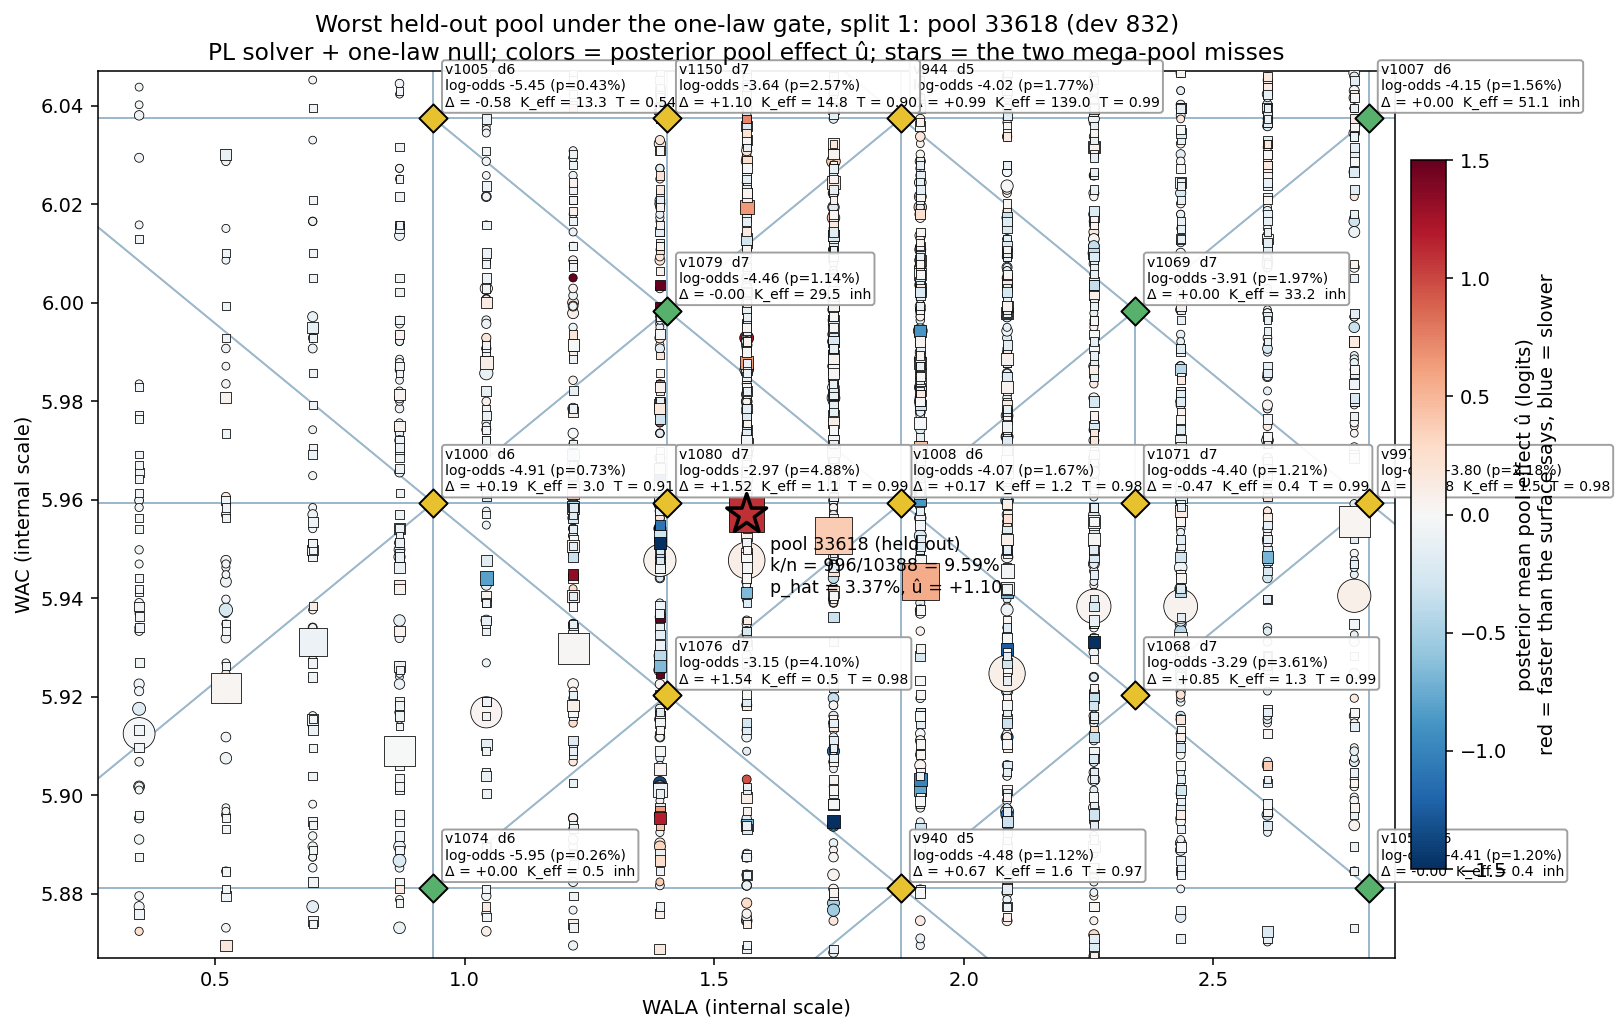
\includegraphics[width=0.95\linewidth]{split1_star_onelaw_worst_pool.png}
\caption{Worst held-out pool under the one-law gate (pool 33618, 10{,}388
loans, observed $9.6\%$ vs fitted $3.4\%$, deviance 832). The failure class
has migrated from invented structure to an honest mega-pool
idiosyncrasy; deviance is large only because exposure is. Note the
one-law gate admitting on thin $K_{\mathrm{eff}}$ where mega pools
dominate: the stratum law variance is near zero there, so one mega pool is
genuinely a lot of evidence.}
\label{fig:star-worst-pool}
\end{figure}

\begin{figure}[H]
\centering
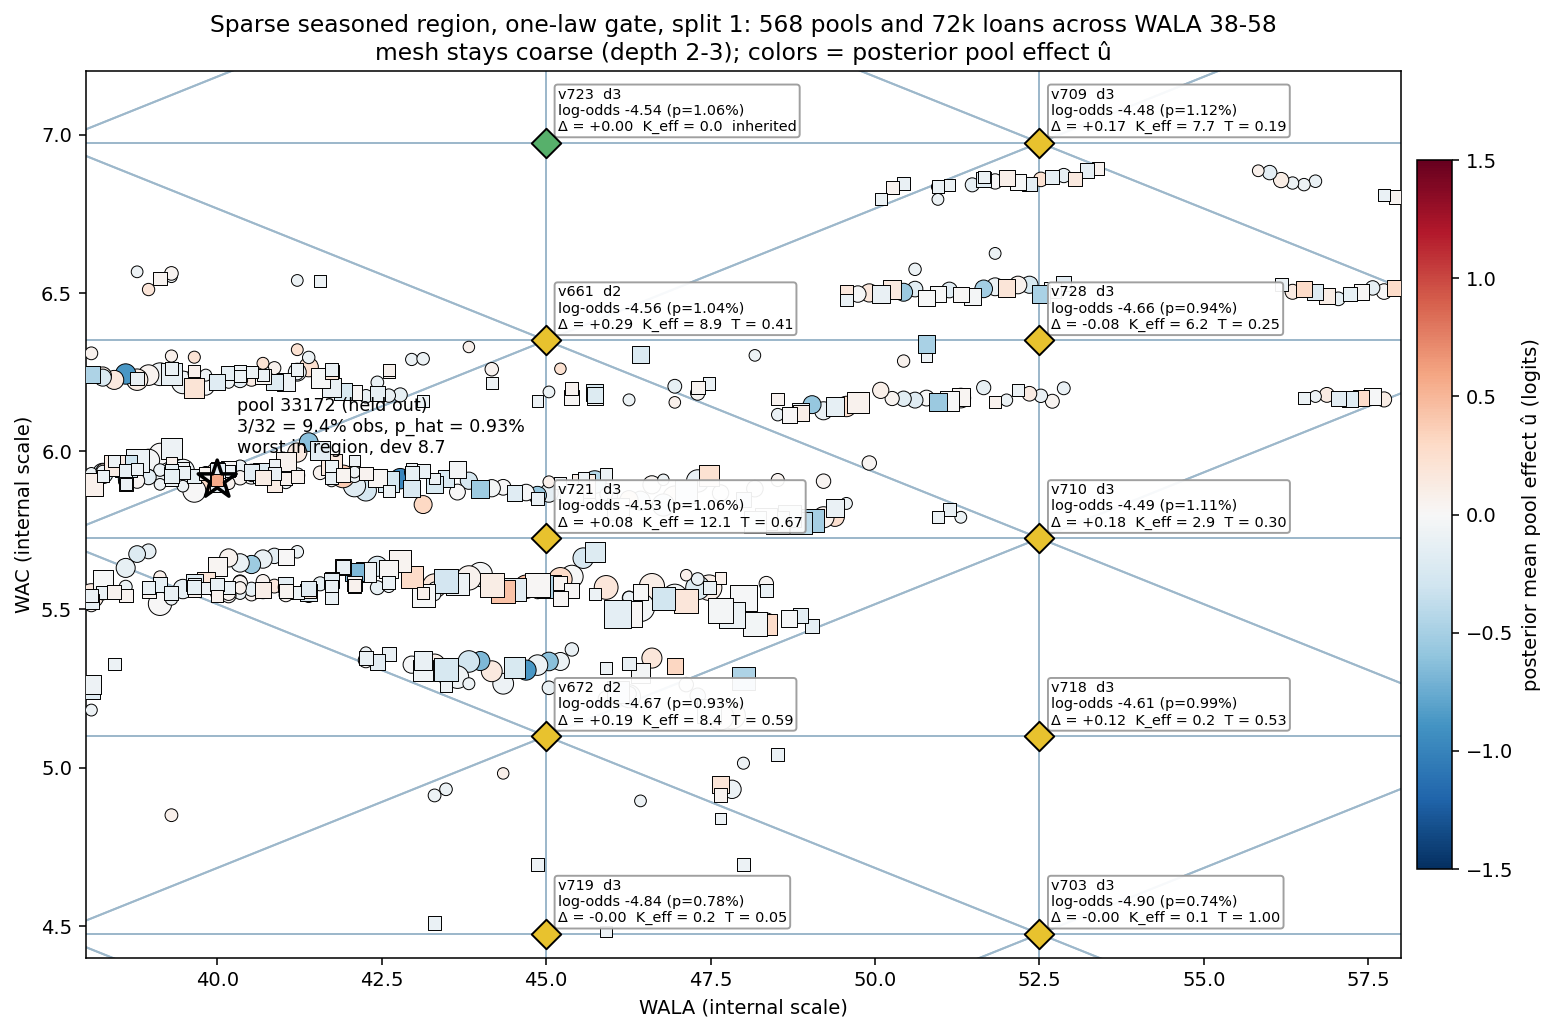
\includegraphics[width=0.95\linewidth]{split1_star_sparse_region.png}
\caption{Sparse seasoned tail (568 pools, 72k loans across twenty internal
WALA units). The mesh stays at depth 2--3, surpluses are tenths of a
logit, and the worst held-out pool in the region costs deviance 8.7: in
sparse territory binomial variance is so wide that wild-looking pools are
weak evidence, and the EB prior contains what the gate admits on thin
support. The system fails safe here.}
\label{fig:star-sparse}
\end{figure}

Two companion figures (Figures~\ref{fig:aug5-2x2} and~\ref{fig:aug5-surface})
document the display corrections adopted during the session: the 2$\times$2 template's held-out panel was rebuilt as a
score-based cell $z$ (the Jeffreys empirical-logit residual, a pre-SMM
holdover, manufactures a spurious fast bias at monthly-SMM rates --- the
program-wide empirical-logit ban applies to displays too), and the fitted
surface acquired a support-honest render: 58\% of the painted area in the
naive render is extrapolation over structurally empty state space (309 of
737 faces hold $\ge 300$ training loans).

\begin{figure}[H]
\centering
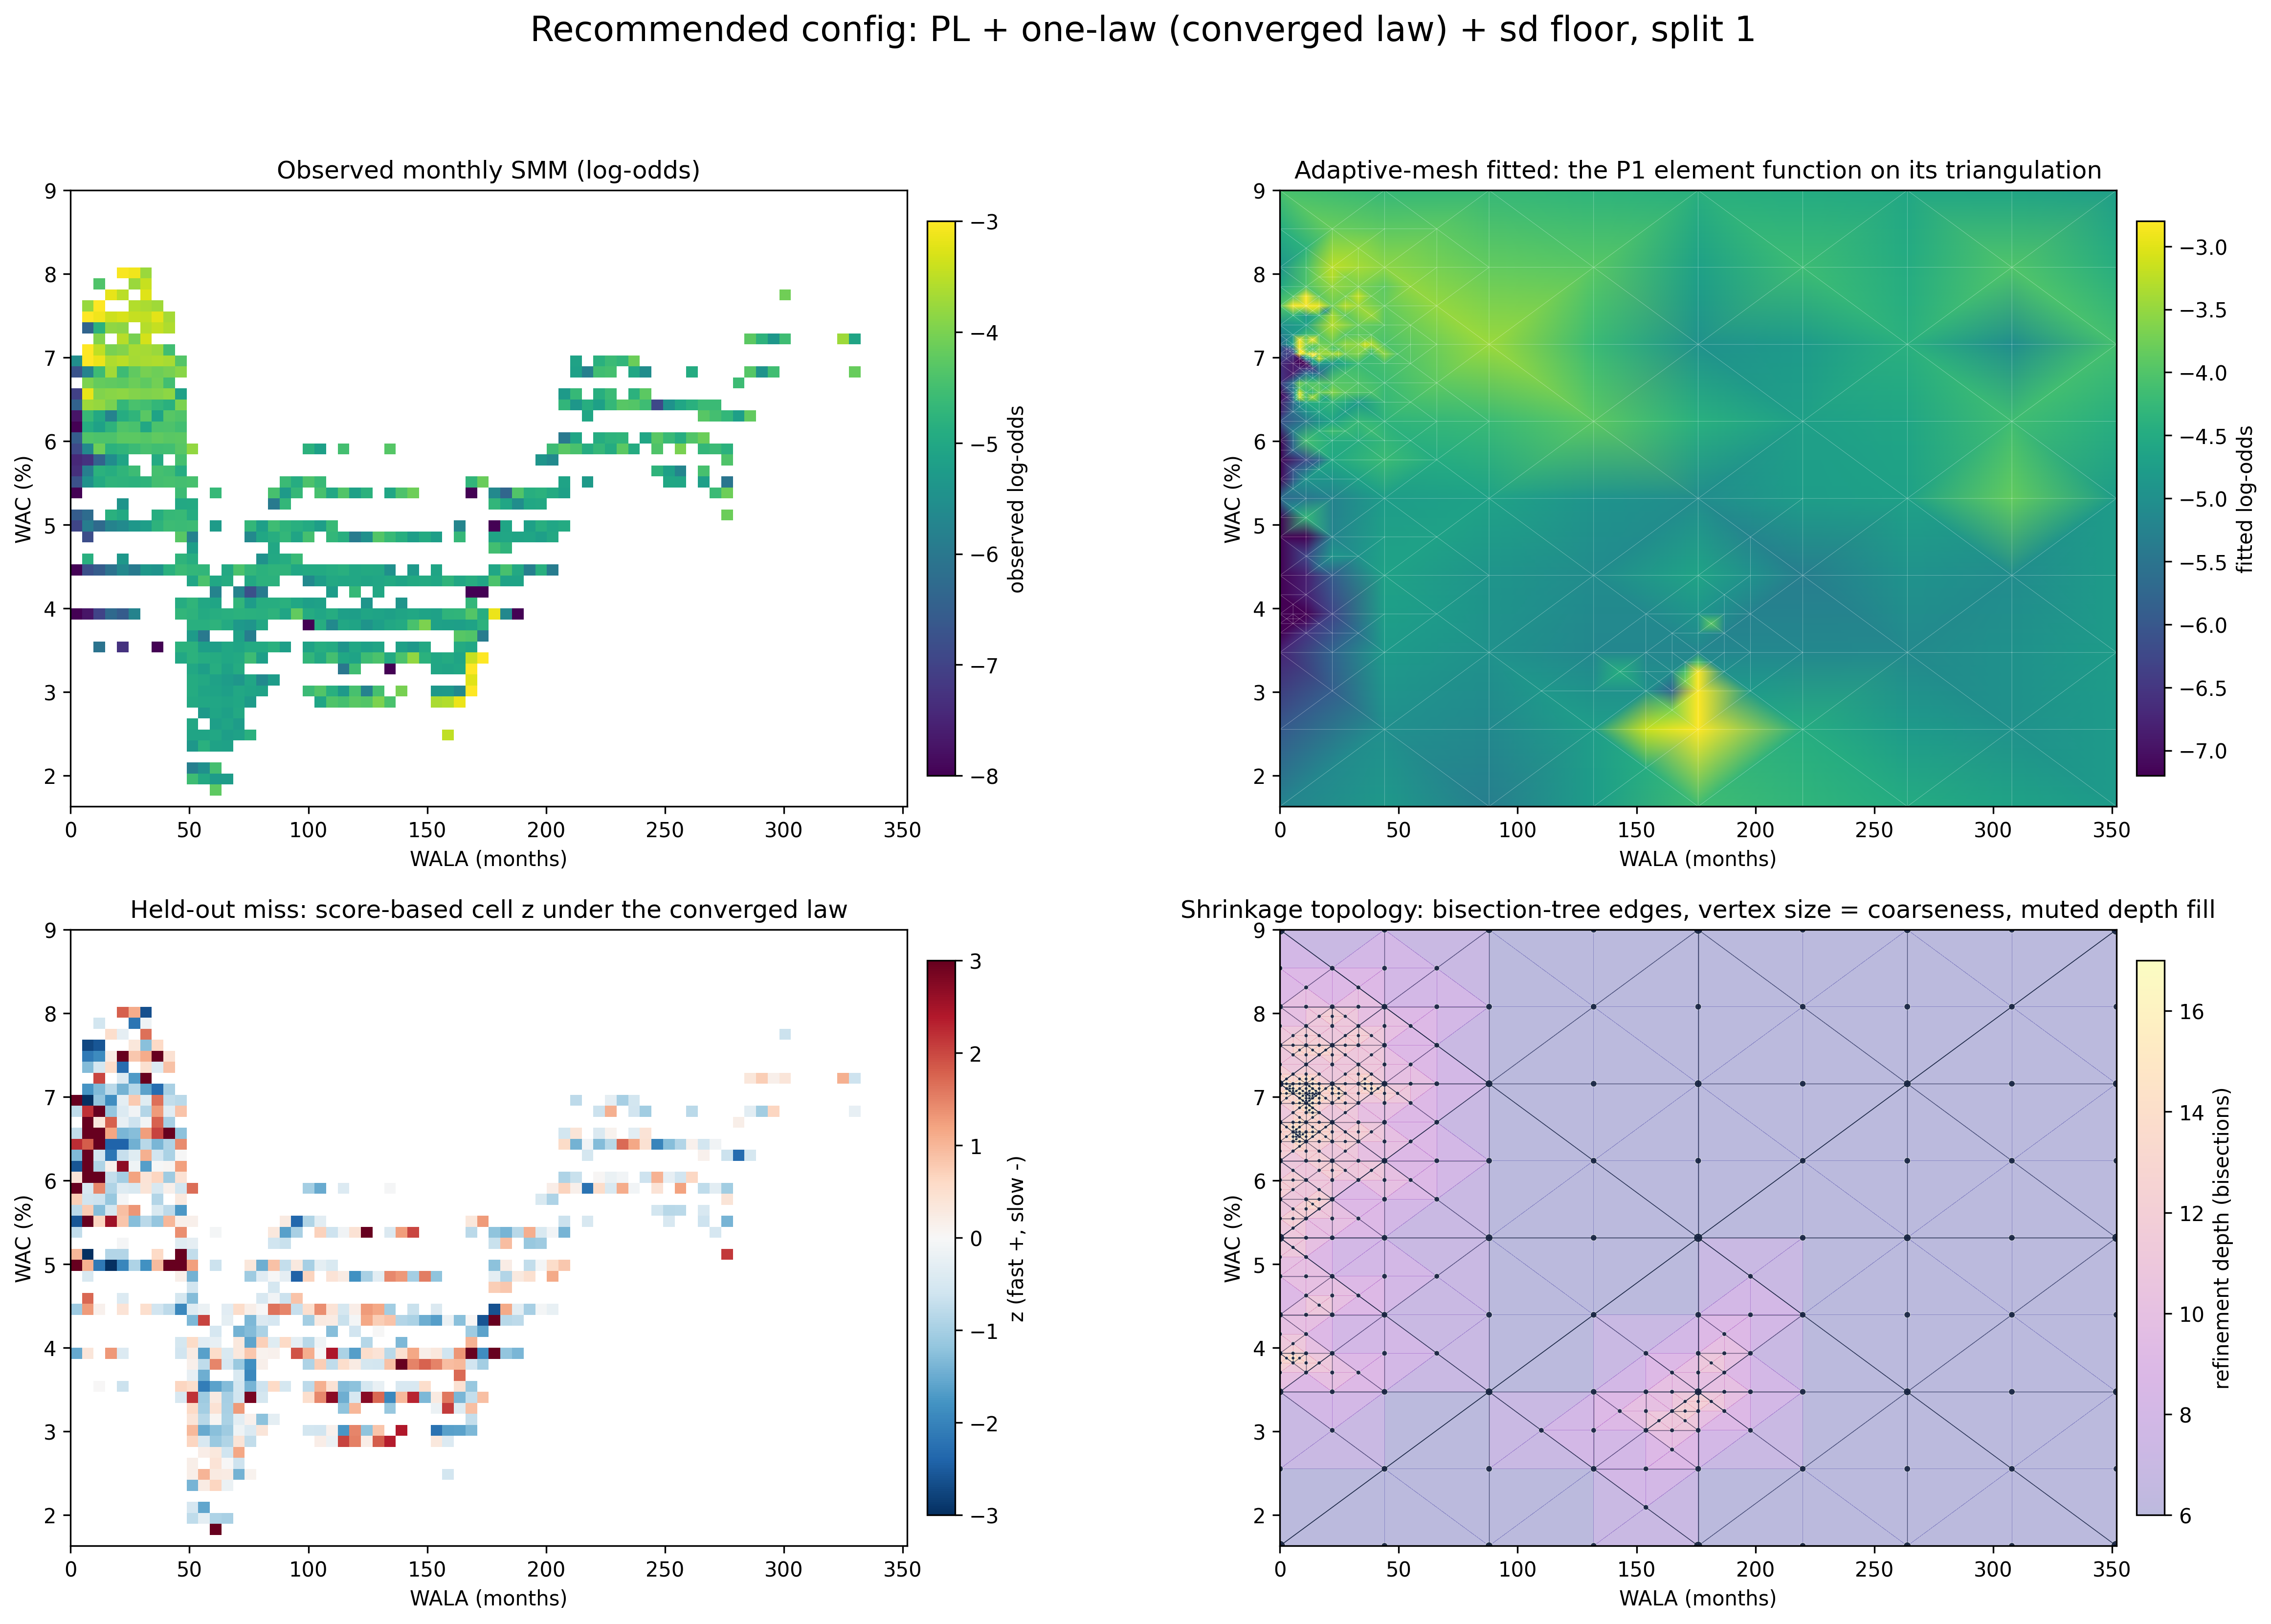
\includegraphics[width=0.97\linewidth]{current_model_2x2.png}
\caption{The 2$\times$2 diagnostic on the recommended configuration
(split 1): observed monthly SMM log-odds, the P1 element function on its
triangulation, score-based held-out cell $z$ under the converged law, and
the bisection topology. The miss panel is two-sided and white-dominated.}
\label{fig:aug5-2x2}
\end{figure}

\begin{figure}[H]
\centering
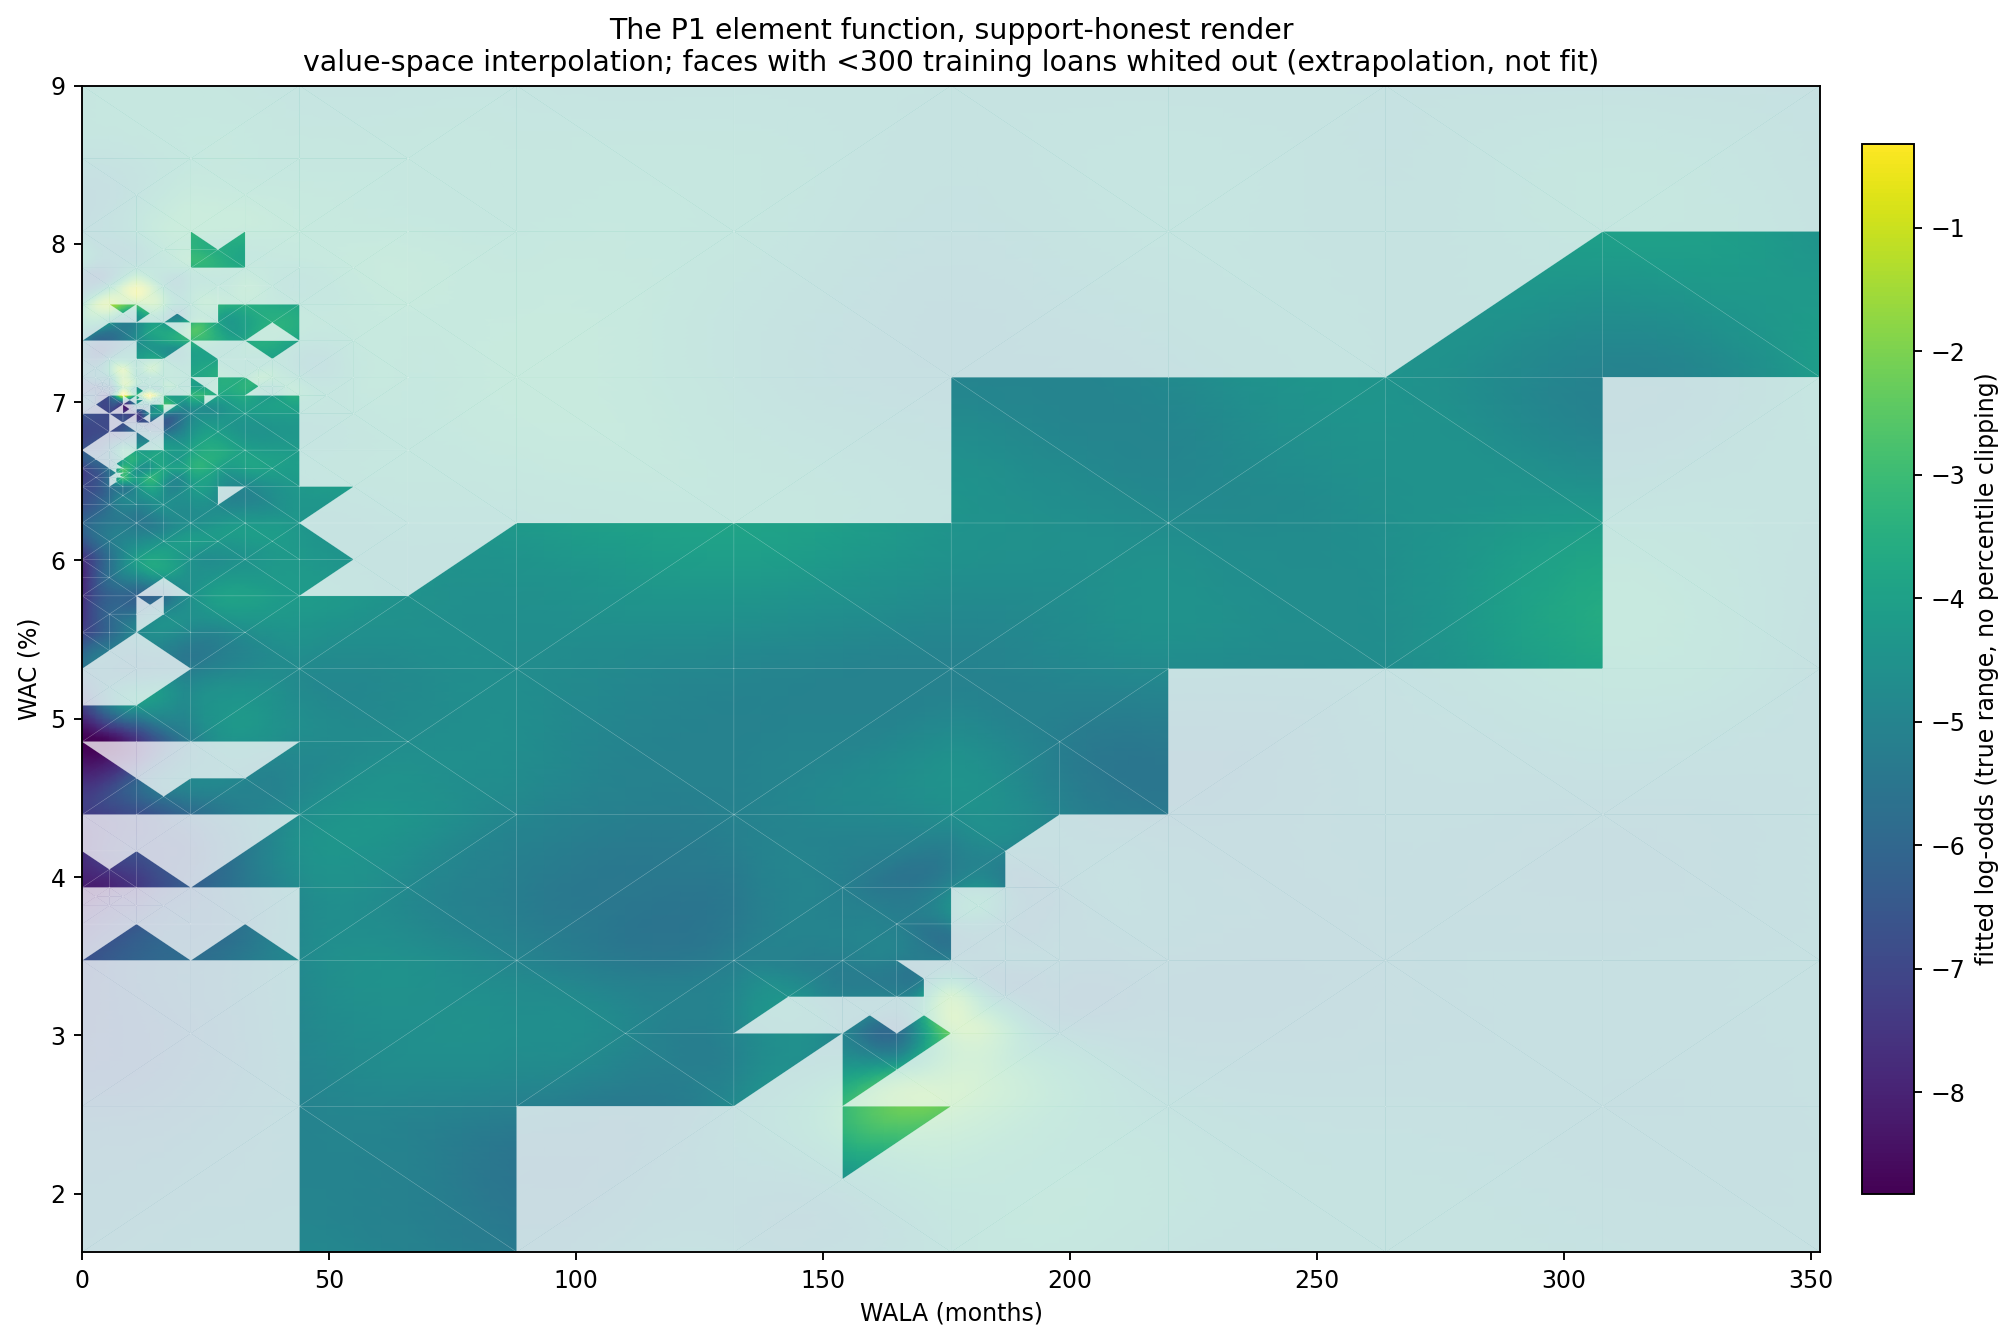
\includegraphics[width=0.9\linewidth]{current_model_surface_honest.png}
\caption{Support-honest surface render: value-space interpolation, true
color range, faces with fewer than 300 training loans whited out. The
supported region is the cohort snake; the fast island at WALA 145--176,
WAC 2.45--3.6 is the 2012--2014 fifteen-year cohort in its amortization
endgame (maturities, de-minimis payoffs, cleanup calls), the least
option-like corner of the surface despite being the fastest.}
\label{fig:aug5-surface}
\end{figure}

\subsection{The ridge counterfactual: the height solve cannot trade surface
for pool effect}\label{sec:aug5-ridge}

The original offending star (pool 33681, $0/376$, the eruption canary)
remains instructive under the recommended configuration
(Figure~\ref{fig:star-offending-rec}): the ridge vertex v1894 carries
$\Delta = +2.06$ at $K_{\mathrm{eff}}=1.39$ with the fit at $23.4\%$
monthly, and the zero-event held-out cluster beside it is one-sided blue
--- the signature of local surface error being charged to the pool ledger.

\begin{figure}[H]
\centering
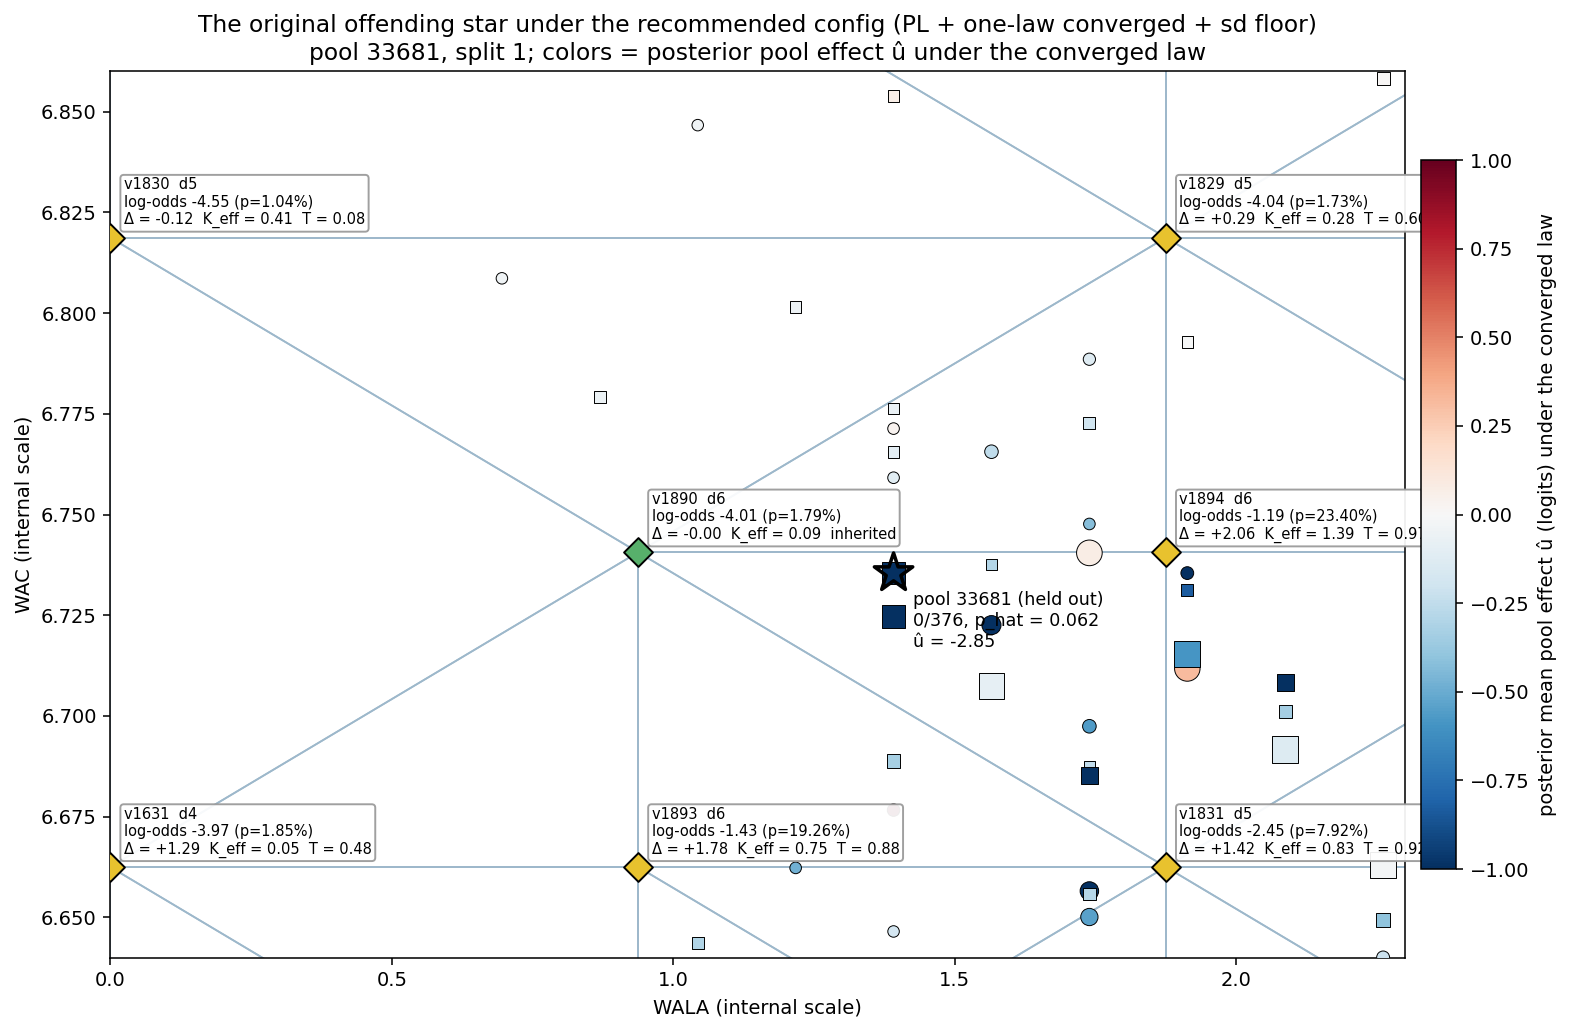
\includegraphics[width=0.95\linewidth]{offending_star_recommended_config.png}
\caption{The original offending star under the recommended configuration.
The eruption is gone (canary at $6.2\%$, not $99.98\%$; pool 33620
ordinary at $\hat u = +0.31$), but the ridge admitted on
$K_{\mathrm{eff}}=1.39$ still overshoots, and the one-sided blue cluster
records the overshoot.}
\label{fig:star-offending-rec}
\end{figure}

A direct counterfactual quantifies the overshoot. Flattening the three
ridge vertices to parent interpolation and scanning the retained surplus
fraction $\alpha$, the held-out mixture log-likelihood over the 30 affected
held-out pools peaks at $\alpha \approx 0.4$ (ridge peak $\approx 8\%$
monthly): the fitted height loses $\approx 23$ nats against that optimum
and fully flat loses $\approx 6$. The elevation is real --- four
independent held-out pools at 5--8\% punish flattening --- but overshot
roughly $2\times$ in log-odds surplus. The training \emph{marginal}
likelihood agrees ($\alpha \approx 0.2$--$0.4$), which localizes the
mechanism precisely: the exact solver maximizes the binomial likelihood
with $u \equiv 0$, so it has no channel through which to charge two logits
of one pool's excess to that pool. Under pure binomial likelihood,
$127/603$ on a $3\%$ surface is impossible and the free vertex must rise;
under the law-marginal likelihood the trade is affordable (the needed
$u=+2.18$ at flat is priced $\sim 10^{-6}$ by the large-pool stratum, but
$u \approx +1.1$ at intermediate height is ordinary) and the optimum
settles where held-out data says the truth is. Status: three-vertex local
scan without refit; the sign and rough magnitude generalize, the 0.4 does
not.

\subsection{Law-marginal final height solve: implementation and
measurement}\label{sec:aug5-marginal}

A frozen-topology law-marginal final pass was implemented as a reference
prototype (\texttt{runs/marginal\_final.py} in the results directory):
joint $(\eta, u)$ ascent under the converged mixture law and the frozen EB
prior, free-vertex coordinate updates with the envelope-theorem score ---
the \emph{untempered} binomial score evaluated at the per-pool posterior
mode --- against the Laplace-marginal curvature $w/(1+w\sigma^2)$, fresh
posterior modes each outer iteration, damped capped steps, and early stop
at the monitored Laplace marginal-likelihood peak (the alternation drifts
past it otherwise; both facts are measured, and tempering the score as
well as the curvature over-flattens, which is the two-currency
fitting-weight mistake in another costume). Topology, admissions, and the
gate are untouched by construction.

On the reference split the ridge lands at $10.2\%$ at the likelihood peak,
independently reproducing the counterfactual optimum
(Figure~\ref{fig:star-offending-marg}); the one-sided blue cluster
dissolves (zero-event held-out $\hat u$ mean $-0.27$ vs $\approx -1.5$
under the binomial solve), and pool 33620 is formally attributed to the
tail component ($\hat u = +1.58$, $\gamma = 1.00$).

\begin{figure}[H]
\centering
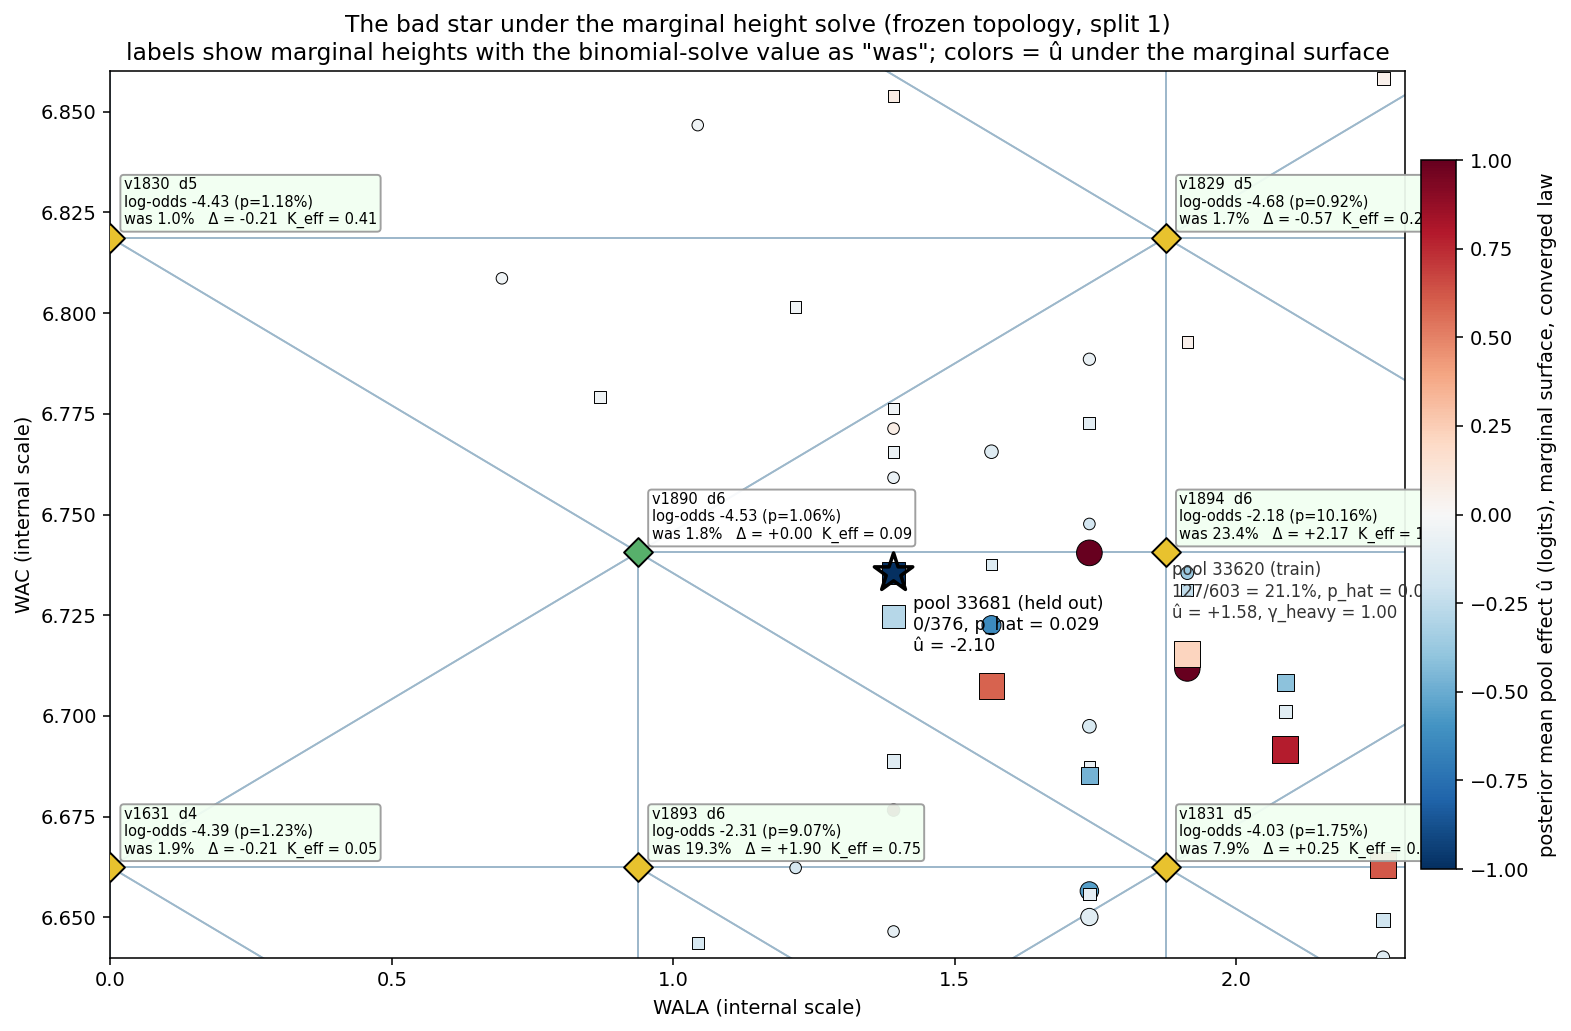
\includegraphics[width=0.95\linewidth]{offending_star_marginal_solve.png}
\caption{The same star under the marginal height solve (frozen topology).
The ridge deflates to its held-out optimum, the surface and the pool
ledger tell one story, and the residual field becomes two-sided and
pool-sized.}
\label{fig:star-offending-marg}
\end{figure}

Measured across splits, on both split conventions:

\begin{center}
\small
\begin{tabular}{lcccc}
\toprule
 & \multicolumn{2}{c}{External masks (diagnostic's)} &
   \multicolumn{2}{c}{Locally balanced (release splitter)}\\
 & held-out dev & mixture NLL & held-out dev & mixture NLL\\
\midrule
naked Lindsey + PL          & 1.1747 & ---     & 1.1482 & 0.92388\\
recommended config          & 1.1893 & 0.93027 & 1.1506 & 0.92423\\
recommended + marginal pass & 1.1979 & 0.92905 & 1.1581 & 0.92201\\
\bottomrule
\end{tabular}
\end{center}

Two findings. First, \textbf{the certification is nearly free under the
program's own split convention}: on locally balanced splits the
recommended configuration matches the naked gate on both instruments
($\Delta$NLL $+0.0004$, $\Delta$dev $+0.002$); the $0.015$ deviance
``price of honesty'' measured on the external masks was largely mask
imbalance. Second, the marginal pass improves the headline instrument on
both conventions and strengthens on the balanced one ($-0.0022$, better
on 7 of 10, largest on the worst splits: $-0.013$ and the boundary-riding
split's deviance by $-0.048$ on the external masks), at a mega-weighted
raw-deviance cost of $+0.0075$. The gains concentrate exactly where
admission instability hurts, so the marginal solve is an alternative
treatment for the boundary-riding problem, not an addition to it. It is
shipped as a reference implementation and analysis tool; promotion into
the C++ coordinate loop --- where it would also reshape admissions rather
than reprice them post hoc --- is the identified next implementation, to
be judged against NLL $0.92201$ on the balanced seeds.

\subsection{Post-hoc all-data optimum at fixed mesh}\label{sec:aug5-oracle}

The same machinery run with held-out pools unmasked gives a per-vertex
oracle: the all-data joint MAP at frozen topology under the same law and
priors --- a diagnostic reference no honest fit matches in expectation.
On the offending star (Figure~\ref{fig:star-offending-oracle}) the ridge
reads $23.4\% \to 10.2\% \to 6.2\%$ across binomial solve, train-only
marginal solve, and oracle: the marginal pass closes most of the distance,
the residual gap is the information content of the held-out outcomes, and
the oracle moves the third ridge vertex \emph{up} (1.8\% $\to$ 4.6\%) ---
disagreement in both directions, the signature of noise-level residual
error rather than systematic bias. Off the ridge, every vertex sits
within tenths of a percent of its oracle.

\begin{figure}[H]
\centering
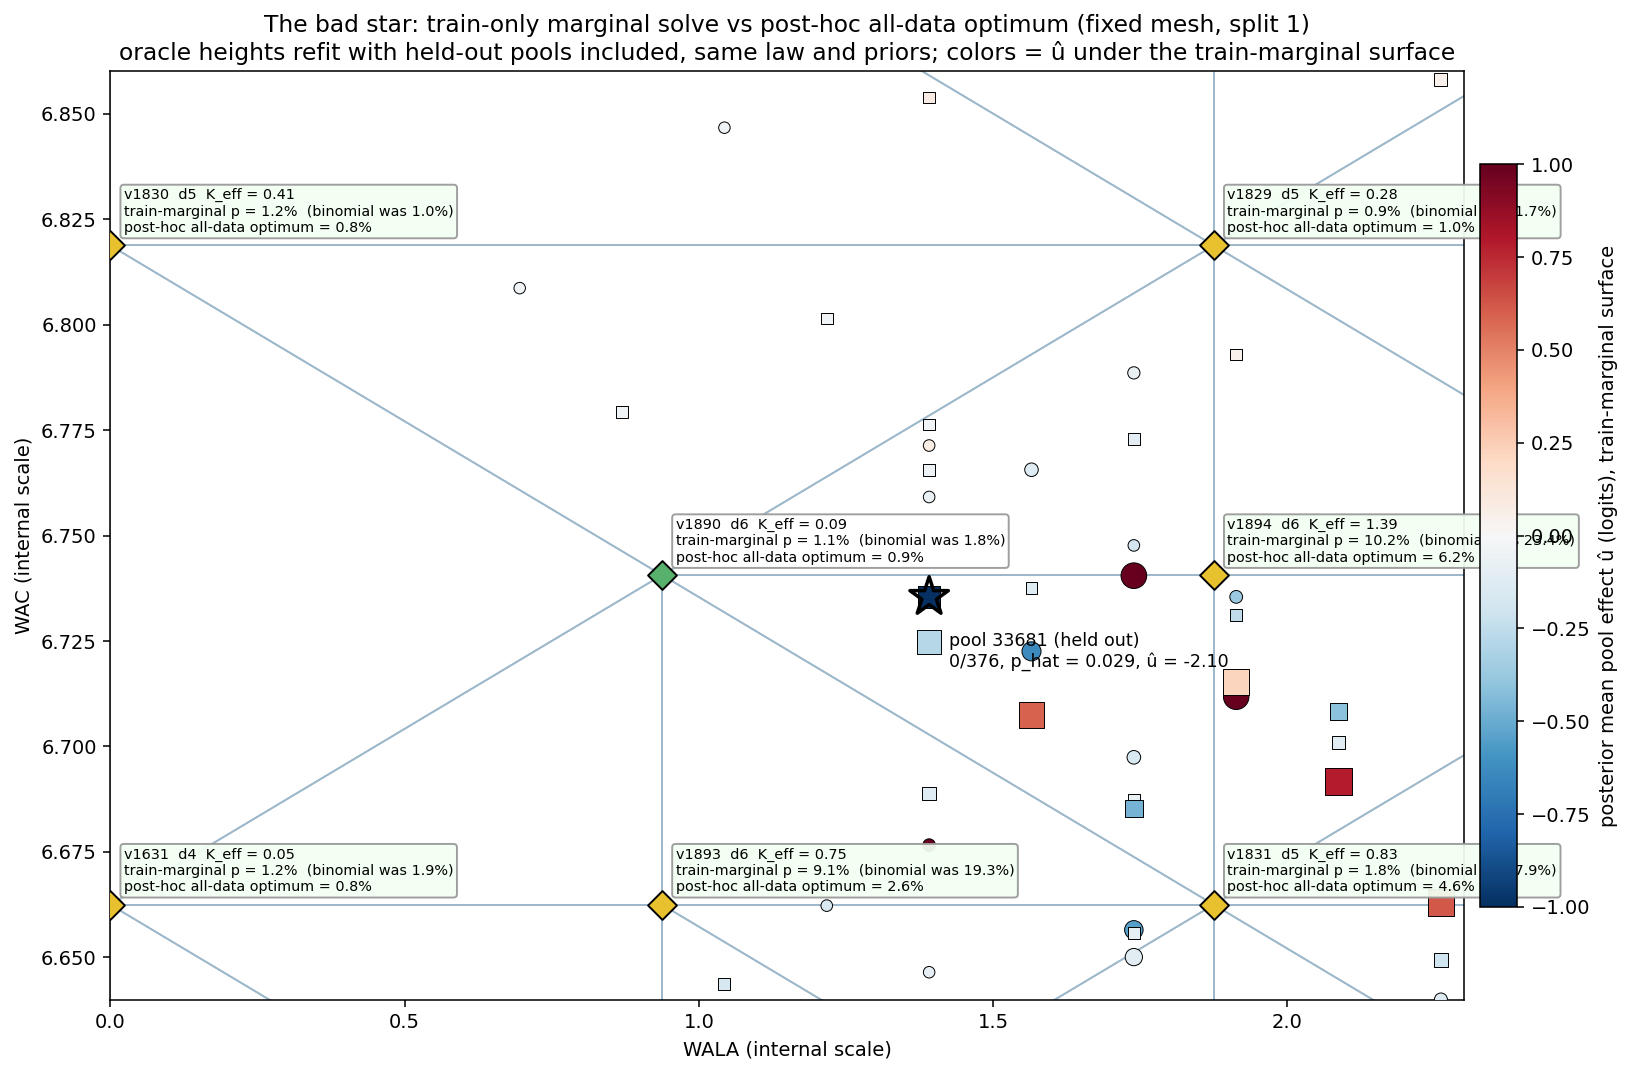
\includegraphics[width=0.95\linewidth]{offending_star_posthoc_optimal.png}
\caption{Train-only marginal solve versus the post-hoc all-data optimum at
fixed mesh. Labels carry three heights per vertex: train-marginal,
binomial (``was''), and oracle. The held-out set's entire information
content in this star is ``the ridge is somewhat lower and tilted'';
away from the ridge the training fit already matches the oracle.}
\label{fig:star-offending-oracle}
\end{figure}

\subsection{Admission churn: measurement and decomposition}\label{sec:aug5-churn}

Status: measured, two independent measurements plus a model-generated benchmark.
The stability open item was quantified directly on the ten locally balanced
seeds under the recommended configuration, in three layers. First, the
algorithm is fully deterministic: same mask, different seed gives bit-identical
vertex files, so all churn is data resampling, none of it algorithmic
randomness. Second, the decision list churns substantially: the admitted
portfolio is majority- or near-majority seed-contingent by evidence weight
(two independent measurements of the same design disagree on the level ---
evidence-weighted core shares of $45\%$ versus $77\%$, location Jaccard
$0.27$ versus $0.53$ --- with the definitional reconciliation pending; both
agree the churn is large). Third, the \emph{surface} is far more stable than
the list: typical-pool cross-seed movement is noise-sized, held-out fit sits
in a tight band, and the excess relative to a fixed-basis GAM on identical
splits concentrates in a small information-weighted tail rather than the bulk.
A spline shrinks every coefficient continuously and never decides; the mesh's
extra resampling variance is precisely the price of discrete, irreversible
admissions near the evidence threshold.

The decomposition question is how much of this churn a correct gate would
exhibit anyway. Benchmark: simulate two worlds from the fitted model itself
(full-data recommended surface plus the converged law, binomial draws), and
run the identical ten-seed battery through the identical pipeline. The
simulated churn is the \emph{power floor}: the resampling distribution of the
decision when the gate is correct and the world is the model.

\begin{center}
\small
\begin{tabular}{lccc}
\toprule
 & real data & sim world 1 & sim world 2\\
\midrule
admission count spread          & $1.7\times$ & $1.2\times$ & $1.4\times$\\
location Jaccard                & $0.53$ & $0.59$ & $0.58$\\
evidence-weighted Jaccard       & $0.386$ & $0.509$ & $0.518$\\
core ($8$+/$10$) evidence share & $77\%$ & $81\%$ & $85\%$\\
singleton evidence share        & $2\%$ & $1\%$ & $1\%$\\
absences with ancestor unproposable & $20\%$ & $8\%$ & $9\%$\\
surface info-wtd cross-seed sd  & $0.080$ & $0.061$ & $0.060$\\
mass with sd $>0.3$             & $4.9\%$ & $0.8\%$ & $0.8\%$\\
\bottomrule
\end{tabular}
\end{center}

Three conclusions. \textbf{(a) Roughly $79\%$ of the measured churn is the
power floor}: a correct gate at this sample size churns half its
evidence-weighted portfolio under half-sample resampling ($J_W=0.51$), so the
benchmark for any stability remedy is the floor, not $1.0$; a remedy tuned
toward perfect reproducibility would be tuned into over-conservatism.
\textbf{(b) The excess ($\approx21\%$) has a located anatomy.} Path dependence
is $2.4\times$ elevated --- one fifth of real absence events are locations
whose ancestors were never proposable in the missing run, versus $8$--$9\%$ at
the floor --- which is exactly the component a two-stage union-topology pass
(build the union of resampled topologies, one final gate pass on the frozen
candidate family) removes by construction. The remainder is
misspecification-flavored and concentrated: the surface is only $1.33\times$
the floor overall but the $>0.3$-log-odds tail is $6\times$ the floor, the
boundary-riding ridge population again; the leading suspect is issuer-block
correlation making half-sample draws effectively noisier than i.i.d., which
ties this residual to the block-exchangeable design of the e-BH certification
route. \textbf{(c) The honest claim is now quantitative}: stable predictions,
stable aggregate honesty guarantees, and individual discoveries that churn at
$\approx1.26\times$ their theoretical floor with the excess concentrated in a
$\sim5\%$ tail. Caveats: two simulated worlds (mutually consistent); the
simulation inherits the fitted surface as truth, which flatters the gate
slightly; and half-sample churn upper-bounds full-sample fragility, since the
shipped fit sees twice the data of any replicate.

\subsection{Outlook: the temporal layer as a weak-form PDE on adaptive
meshes}\label{sec:aug5-temporal}

Status: design, nothing in this subsection is measured. The program's end
goal is forecasting, and the data shape dictates the architecture: many
spatial points per month ($N \approx 33{,}740$ pools) but few usable time
points ($T$ in the dozens, broken by rate regimes). Time provides no
averaging; every cross-sectional defect becomes a permanent feature of the
time series, and at small $T$ a spurious admitted feature is statistically
indistinguishable from a real factor. The spatial gate is therefore doing
temporal work: FDR control in space substitutes for the replication that
$T$ cannot supply, and each admission decides what is allowed to become a
time series.

The temporal design deliberately does \emph{not} freeze the mesh across
months. A frozen topology couples every month's capacity allocation to the
first month's evidence and makes the state dimension the vertex count,
unestimable at small $T$. Instead each month's mesh remains fully adaptive
and months are coupled through the weak formulation: the dynamics is posed
as a relatively simple linear second-order (parabolic) PDE
\[
\partial_t \eta \;=\; \nabla\!\cdot\!(A\nabla\eta) \;-\; b\!\cdot\!\nabla\eta
\;+\; c\,\eta \;+\; f(x,t),
\]
tested against a fixed dictionary of test functions $\varphi_j$. The
monthly fits enter only through the moments
$\langle \varphi_j, \eta_t\rangle$ and
$\langle \nabla\varphi_j, \nabla\eta_t\rangle$, which are exact
triangle-by-triangle integrals of a P1 function against smooth
$\varphi_j$ on \emph{whatever mesh month $t$ built} --- no node
correspondence is ever needed. The semi-discretized weak dynamics is then
linear regression of moment increments on moment functionals across
$(j,t)$, with $O(10)$ operator coefficients against $T$ observations of a
33k-point field: the one regime in which small $T$ is comfortable.

The cross-sectional honesty apparatus becomes, literally, the weight
matrix of the dynamics. Each moment is a linear functional of the vertex
heights, so its sampling variance is $a_j^{\top}\Sigma_t a_j$ from the
fit's posterior covariance (under the marginal solve, the inverse of the
tempered curvature), and the PDE coefficients are estimated by GLS with
those weights, honestly errors-in-variables on both sides. Uncertain
months and uncertain scales penalize themselves.

Two structural properties of this state space are imposed, not estimated.
The advection coefficient is known: WALA ages one month per month
deterministically and WAC is static per pool, so $b=(1,0)$ is fixed and
the null model of the temporal layer is \emph{pure transport} --- the
surface constant in vintage coordinates. Whatever the diffusion, decay,
and forcing terms then earn is certified behavioral dynamics beyond
aging, with the forcing naturally parameterized through the known
incentive covariate $\mathrm{WAC}-r_t$, keeping the operator linear in
its parameters. And the domain has a genuine inflow boundary: new
issuance enters at $\mathrm{WALA}=0$, so the issuance edge is boundary
data --- where new information physically enters the PDE --- while the
amortization endgame at term is the outflow.

Finally, the decision framing survives the change of layer intact. The
choice of test dictionary is the temporal admission problem: each
$\varphi_j$ defines a scalar time series with known measurement noise, so
whether a spatial scale receives dynamics is a gateable decision ---
signal against noise, FDR over test functions --- and coarse dictionaries
automatically integrate out the admission-flicker halo that should never
be forecast. One discipline is mandatory at this $T$: the test dictionary
must be fixed and pre-registered before any temporal fits are examined,
in the same way the certified windows were predeclared, because adaptive
test-function selection at $T \approx 36$ would rebuild in time exactly
the selection disease the spatial program spent this audit curing.

\subsection{Reproduction}
Everything in this section regenerates from the release tree: the design is
\texttt{data/smm\_design\_202606.csv}; the external diagnostic masks and the session's
result tables, figures, and scripts are under
\texttt{results/aug5\_pl\_onelaw\_audit/} (masks in \texttt{mc10\_split\_masks/},
the marginal solver as \texttt{marginal\_final.py}, session narrative in
\texttt{SESSION\_NOTES\_2026-08-05.md}); the binary rebuilds from \texttt{core/} with
CMake. The recommended configuration is the three environment lines of the state page;
locally balanced splits use \texttt{DMESH\_SPLIT\_MODE=local} with the seed as the fifth
positional argument, external masks replay through \texttt{DMESH\_SPLIT\_MASK}.

\subsection{Open items}
Consolidated with the program-wide list in Section~\ref{sec:discussion}, which
supersedes per-section lists.

% ---------------------------------------------------------------------------
% August 6 session: regime transfer, the simulation program, anatomy of a
% false certification, and the release rule.  Inserted 2026-08-06.
% ---------------------------------------------------------------------------
\section{August 6 session: regime transfer, known-truth simulation, anatomy of a false certification, and the release rule}\label{sec:aug6}

This section records a single extended session (August 5--6, 2026) on the 2020
COVID refi-wave regime and on the certification machinery itself. Its
deliverables: (i) a two-regime panel with a standing \emph{law fixed-point per
regime} rule and one retraction; (ii) a known-truth simulation program that
calibrates the solver's reported uncertainty and adjudicates the shrinkage
design; (iii) a complete causal account of one false certification, from
admission through redistricting to repair, with the constrained-closure
mechanism and its local-release cure demonstrated on real data; (iv) a
release-rule design with full-mesh censuses, a two-currency principle with
measured teeth, and a first working hierarchical (two-groups) trust layer that
produces the best held-out surface of the session. Status labels throughout:
\textsc{measured} (numbers from data or simulation), \textsc{design} (agreed
specification, not implemented), \textsc{retracted}.

\subsection{The 2020 regime: transfer, the law fixed point, and a retraction}
\label{sec:aug6-regime}

\textsc{Measured.} All twelve 2020 monthly SFPS files parse and transport
cleanly (225--238k pools/month, 11 transitions, zero negative loan-count
drops). Wave-regime persistence is structurally different from 2026:
attenuation-corrected signal correlations $0.795/0.651/0.570/0.487$ at lags
$1/2/3/6$ imply a near-fixed frailty component ($\approx$45--50\% of signal)
against 2026's AR$(1)$-like $\rho\approx0.65$; signal is 75\% of pool residual
variance in both regimes. The stage-boosting chain transfers with a frozen
tournament ordering and per-month stage gates, with gains 2--3$\times$ the
2026 scale.

\textsc{Retracted.} The initial finding that the chain \emph{loses} the
June$\to$July and July$\to$August 2020 transitions (the delinquency-buyout
months) was a law artifact. Refitting the SMM pool-law fixed point on the 2020
regime (per-stratum totals $0.151/0.254/0.126/0.049$ against 2026's
$0.143/0.242/0.029/0.004$; the mega-pool strata carry $4$--$13\times$ the 2026
variance) and re-running gates and scoring under the 2020 law flips
June$\to$July to a $+0.093$ NLL win. The buyout-months story is downgraded to
at-most-deviance-neutral. Standing rule: \emph{the law fixed point is
per-regime and per-model} (including post-boosting refits; the boosted chain
absorbs $\approx$77\% of pool-effect variance, leaving the 2026-calibrated law
$\approx4\times$ too large); pinning a law across regimes converts law
misspecification into fake structural conclusions.

\subsection{Known-truth simulation and the honest-uncertainty stack}
\label{sec:aug6-sims}

Two worlds built on the real January-2026 design geometry (real coupon
lattice, sizes, issuer labels; truth surface from a fitted field): world A
with the exchangeable converged law; world B with issuer-block effects (sd
0.30) plus a reduced individual law. \textsc{Measured} verdicts:

\begin{itemize}[leftmargin=2em,itemsep=2pt]
\item \textbf{The reported $\sigma^2$ is optimistic everywhere.} Claimed
coefficient standard errors understate realized error $2.21\times$ in the
\emph{perfectly specified} world A (joint-fit correlation plus selection) and
$3.18\times$ under blocks. The dominant term is joint-fit correlation, not
winner's curse: reading contrast variances off the full penalized-information
inverse restores $\mathrm{sd}(z_{\mathrm{err}})=1.13$ in world A; adding a
law-plus-block sandwich $\Omega$ restores $1.12$--$1.35$ in world B.
\item \textbf{Gate error rates.} False admissions 27\% in world A (an upper
bound under the approximate null definition), 36\% under blocks. A two-groups
audit on sandwich-honest $z$'s removes 42--45\% of false admissions at
85--87\% retention; the same audit on claimed $\sigma^2$ removes 6\%.
\item \textbf{Coarseness is the identifiability defense.} Only 5\% of the
injected block effect leaks into the fitted surface (13\% for spatially
concentrated blocks, 3\% diffuse); the mesh refuses blocks to the pool layer
and the law prices what is refused. Block-aware nulls are targeted cleanup,
not global repair; the pool-layer/panel treatment is where refused variance
becomes forecastable signal.
\item \textbf{The fair fight.} Frozen-topology joint re-solves differing only
in $\Lambda$: depth-based shrinkage ties the honest two-groups prior for point
estimation in both worlds (oracle wMSE $0.0156$ vs $0.0154$;
$0.0455$ vs $0.0448$). Sophistication's proven value is calibrated
uncertainty and audit power, not primary-plane point estimates.
\item \textbf{Post-hoc coordinatewise re-shrinkage is refuted.} Applying
audit-derived shrinkage marginally degrades the surface catastrophically
(world A oracle wMSE $0.033\to0.159$): coefficients are fitted jointly and
their errors cancel; marginal edits break the cancellation. Shrinkage may
enter only through $\Lambda$ inside the joint solve.
\end{itemize}

Separated deliverables: (a) in-loop se fix (contrast variances off the
existing factorization, sandwich $\Omega$) --- ship; (b) two-groups $q$'s as a
post-hoc \emph{audit} overlay --- usable now; (c) prior upgrades in-loop only;
(d) post-hoc surface editing --- never.

\subsection{Anatomy of a false certification}\label{sec:aug6-anatomy}

The June$\to$July 2020 fit certifies a $+4.43$-logit surplus ($9\sigma$
against reported se, trust $T=0.95$) at a coupon-lattice corridor vertex,
rendering 25.2\%/month over pools whose hat-weighted evidence is
1.09\%/month. The session traced this object end to end; every intermediate
hypothesis was tested and most died.

\paragraph{Static forensics (\textsc{measured}).} The vertex's heavy voters
are zero-event pools ($k=0/43,0/84,0/63,\ldots$); the fast pools in its ring
are low-hat fringe members of neighboring coupon columns. The lineage
sawtooths ($-2.20$, $-2.01$, $+4.43$, each ``significant'' marginally,
jointly a modest field): coordinatewise audits certify teeth, not the bite.
A one-coordinate height sweep under the tail law leaves 23.8 nats on the
table (31.5 binomial) against the parent level. Eliminated: robustness
plateau, prior anchoring (prior means are zero for all 118 admissions),
dump-column confusion (the \texttt{height} column reproduces shipped
$\hat p$ to $R^2=1.000000$), staleness (a final exact frozen-topology refit,
\texttt{DMESH\_HIER\_FIT=2}, moves nothing), and temper distortion (a
law-GLS re-tempered final solve, \texttt{DMESH\_LAW\_WEIGHTS\_FINAL=1},
moves \emph{other} vertices but not this one).

\paragraph{Mechanism: the constrained-closure compromise (\textsc{measured}).}
The vertex carries four conformity-welded midpoint descendants (no
coefficients), so its exact design column spans a footprint of 36 extra train
pools (1{,}872 loans at 5.50\%/month) beyond its one-ring (18 pools, 749
loans, 2.67\%/month). The hot constrained footprint outvotes the corridor;
the compromise is rendered where the losing population lives; the solver is
converged. One knob, two rooms (Figure~\ref{fig:aug6-tworooms}). This is the
third basis-level disease after boundary anisotropy and lattice voids, and it
has a certification corollary: \emph{a certificate must quote a coefficient's
footprint through its constrained children, not its one-ring}.

\begin{figure}[t]
\centering
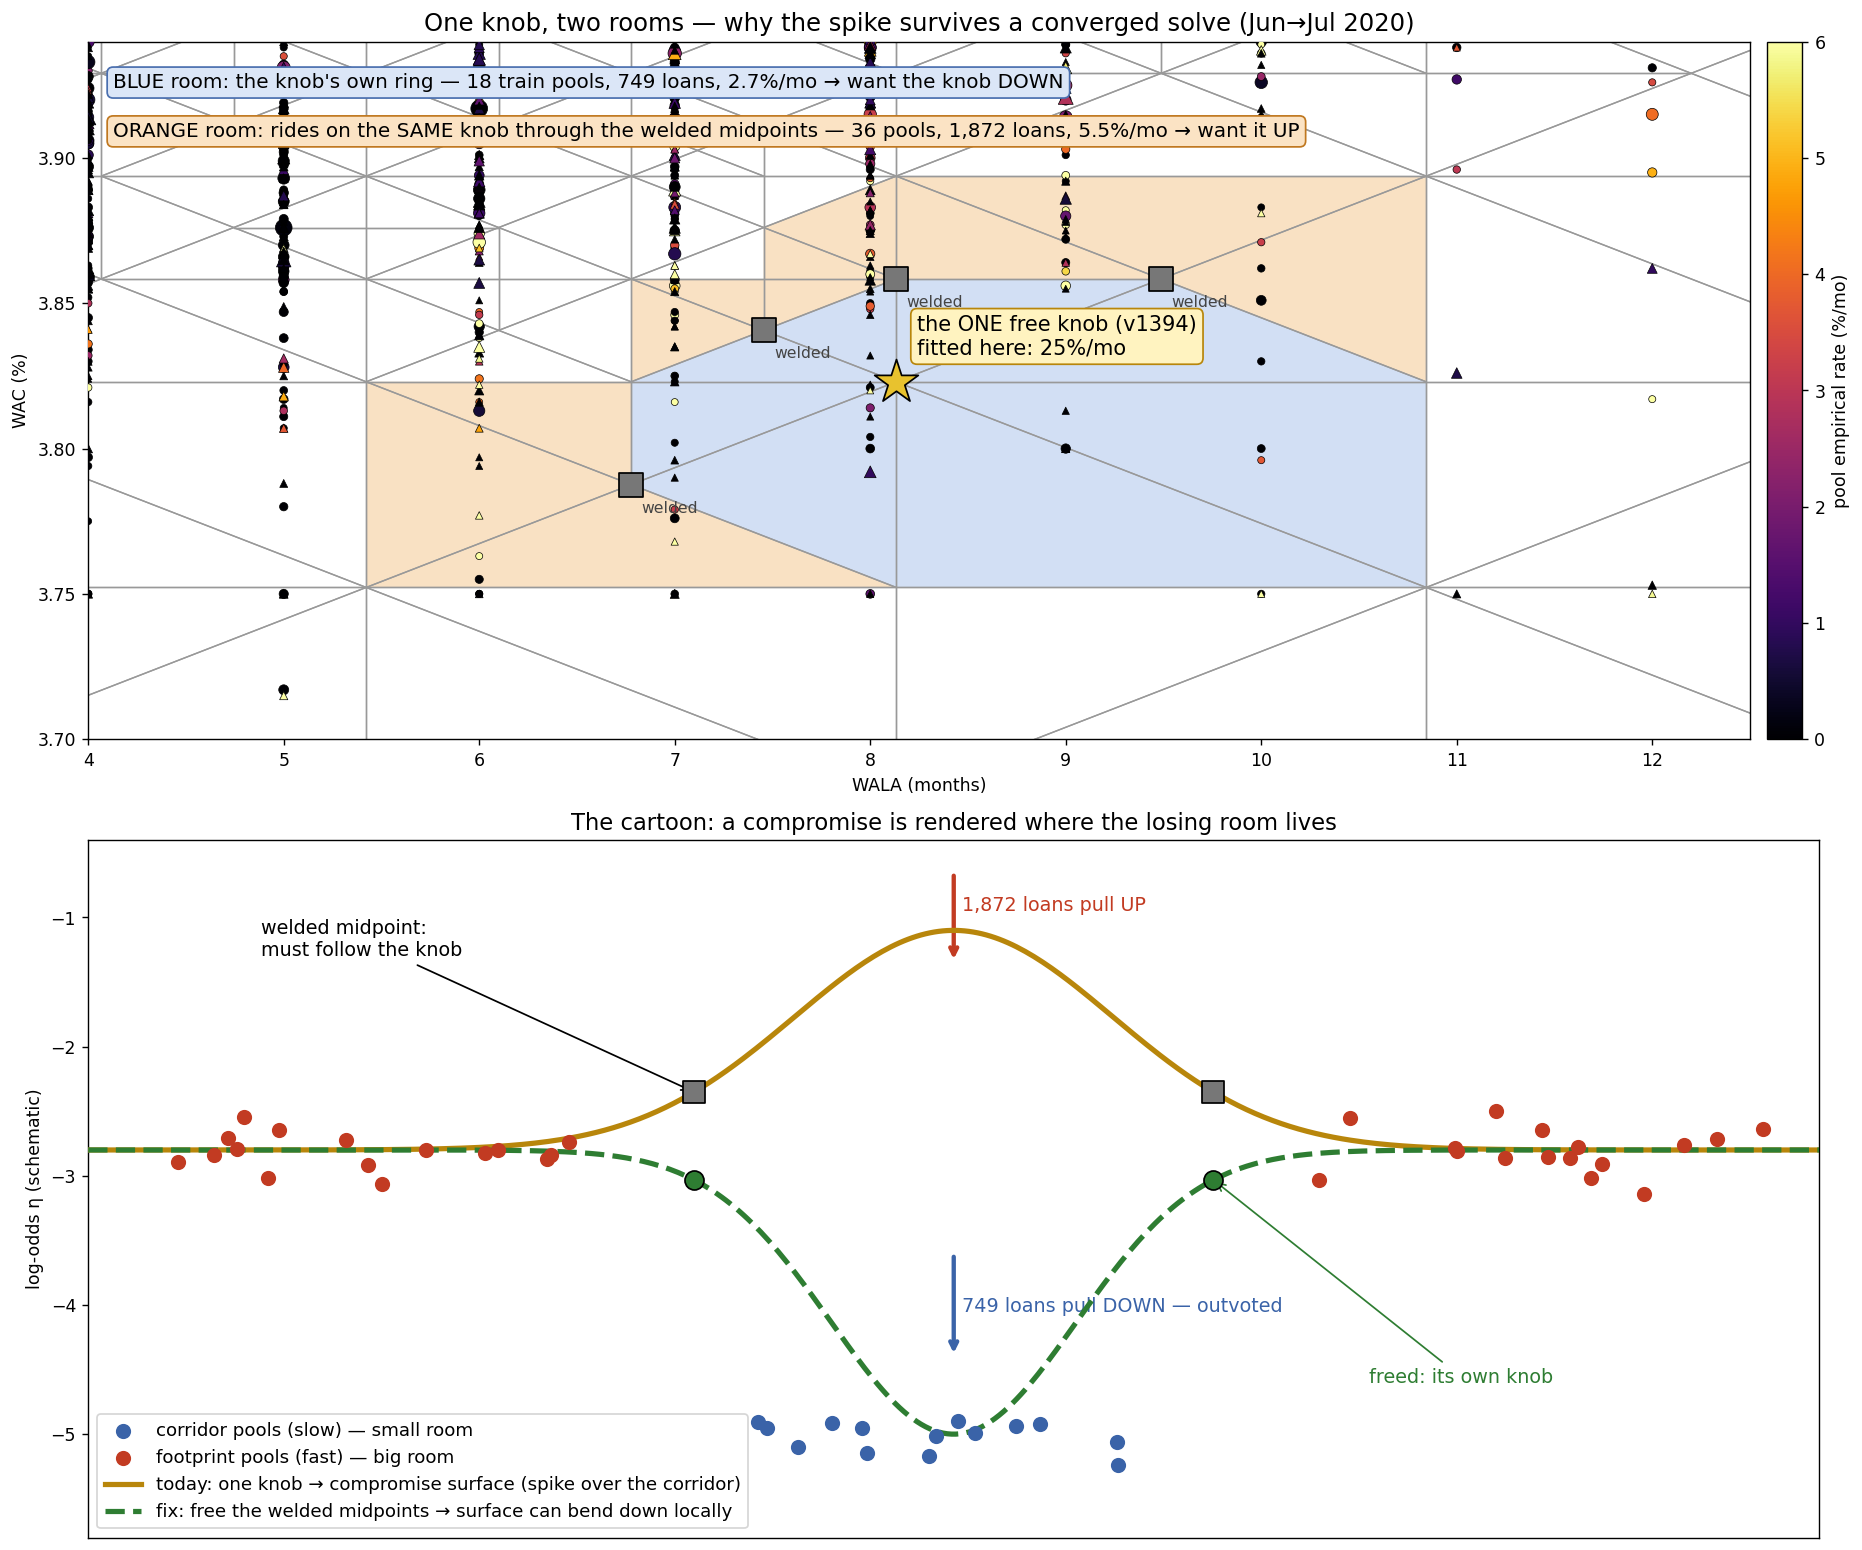
\includegraphics[width=0.92\textwidth]{one_knob_two_rooms.png}
\caption{The constrained-closure compromise. Top: the real region; marker
area is vote share at the certified vertex, color is empirical rate; the
one-ring (blue room) wants the coefficient down, the constrained footprint
(orange room) rides the same coefficient through welded midpoints and wants
it up. Bottom: schematic; the compromise surface is rendered over the losing
room, and freeing the welded midpoints lets the surface bend.}
\label{fig:aug6-tworooms}
\end{figure}

\paragraph{History: the gerrymander (\textsc{measured}).} Round-capped
snapshot refits (\texttt{DMESH\_MAX\_GATE\_ROUNDS} +
\texttt{DMESH\_STOP\_AFTER\_ADAPTATION}, vertex tracked by coordinates)
recover the biography (Figure~\ref{fig:aug6-filmstrip}): promoted at round 5
at $\eta=-1.82$ serving 97 pools/5{,}934 loans at 3.6\%/month (raw data pull
$+0.82$ logits; defensible); successive refinements carve the ring
$97\to48\to26\to18$ pools with pooled rate swinging
$3.6\to5.2\to8.2\to2.7$\%/month; the height never re-adjusts while welds
accumulate one to five. Elected by one constituency, redistricted into its
opposite, prevented from resigning. The one-coordinate relax dual (below)
already reads $+14.6$ train / $+35.4$ held nats at round 5: the compromise
predates the carving, and a per-carve ``redistricting review'' would have
flagged it five rounds early.

\begin{figure}[t]
\centering
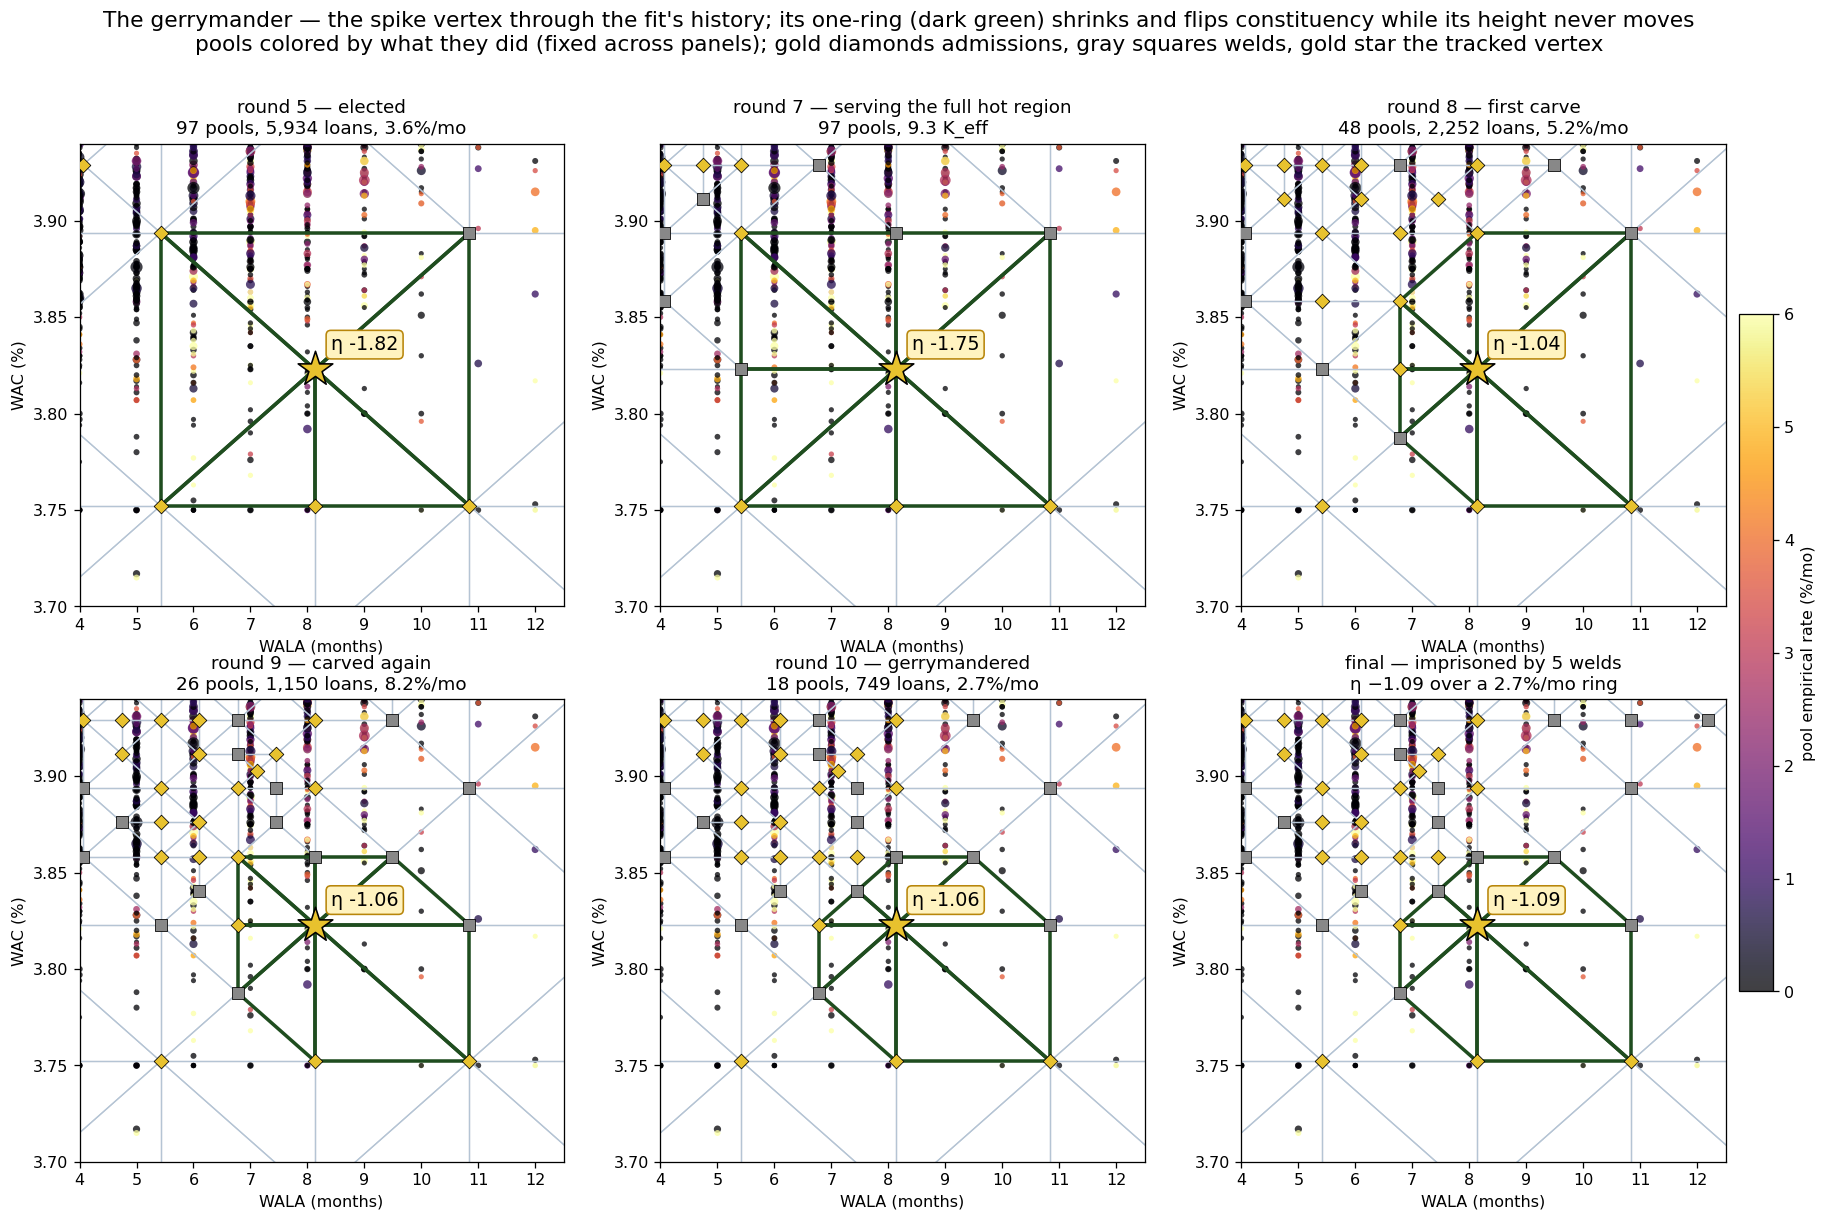
\includegraphics[width=\textwidth]{spike_history_filmstrip.png}
\caption{The gerrymander. Six exact snapshots of the region; the tracked
vertex's one-ring (dark green) shrinks and flips constituency
(3.6$\to$5.2$\to$8.2$\to$2.7\%/month) while its height stays fixed and welds
(gray) accumulate.}
\label{fig:aug6-filmstrip}
\end{figure}

\paragraph{Repair: local release (\textsc{measured}).} Freeing the four welds
and re-solving only those five heights (coordinate ascent on the law-marginal
train likelihood, $\tau=1$-logit prior toward parent interpolation,
everything else frozen): the knob moves $-1.09\to-4.42$, landing at the
ring's hat-weighted evidence ($-4.50$; the pre-registered bar was ``$-4.5$
or below,'' missed by 0.08 and flagged); region train likelihood $+31.5$
nats, \emph{held-out} $+37.9$ nats. The blue room's 16 held-out pools go
from deviance 6.27 (2.2$\times$ the month average) to 1.37 (better than
average); the orange room's held-out $z$ improves $-1.87\to-0.57$; full-month
held-out deviance improves $+0.0049$ from five numbers
(Figure~\ref{fig:aug6-after}).

\begin{figure}[t]
\centering
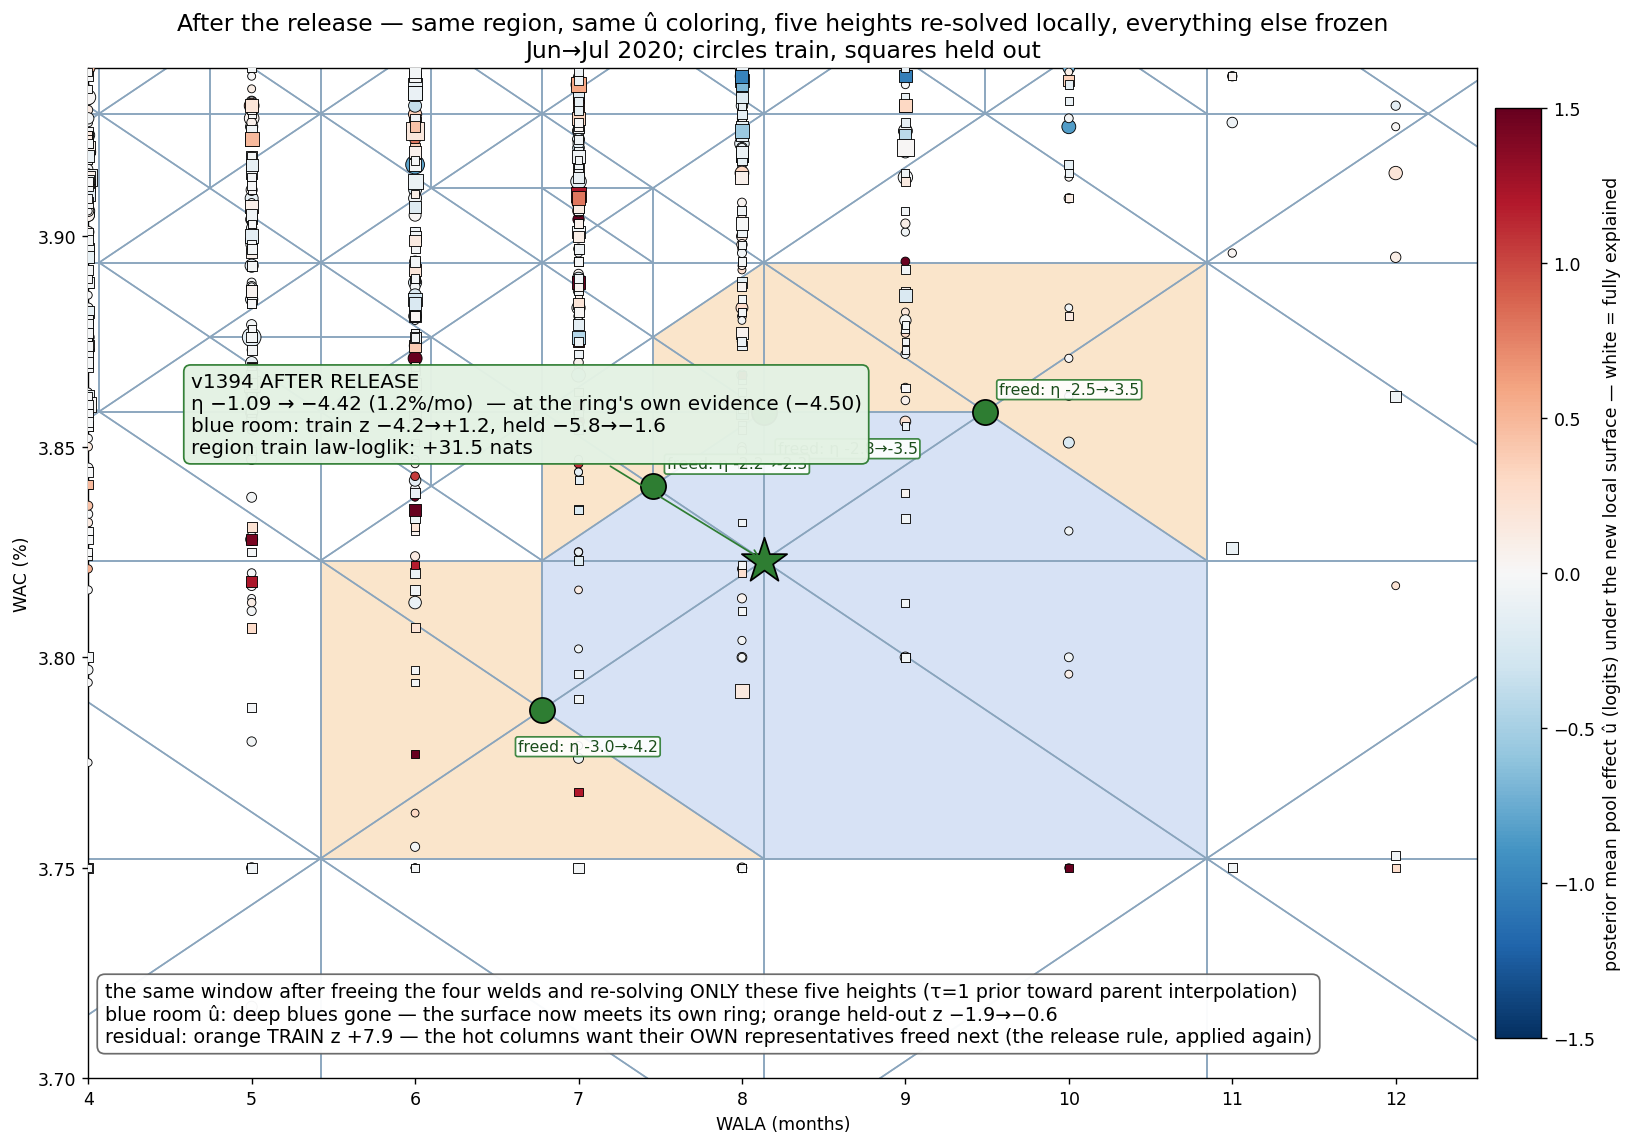
\includegraphics[width=0.94\textwidth]{void_spike_after_release.png}
\caption{After the five-height local release: credibility posteriors
$\hat u$ under the new local surface. The coherent blues under the certified
vertex are gone; the freed midpoints (green) settle at their own rooms'
levels.}
\label{fig:aug6-after}
\end{figure}

\subsection{The release rule, the censuses, and the two-currency principle}
\label{sec:aug6-release}

\paragraph{Design (\textsc{design}, agreed).} Welded midpoints and unproposed
candidates are the same object: linearity constraints. Decouple geometric
status \{absent, present-conforming\} from statistical status \{constrained,
free\}, price every constraint by its one-ring score multiplier through the
same gate (releases enter the e-BH budget; winner's curse applies), allow
release and re-weld transitions, re-audit footprints and re-score greedily
between releases, and trigger re-pricing on every ring-changing refinement.

\paragraph{Censuses (\textsc{measured}).} Weld census, June$\to$July: 119
welds, 99 scoreable; 16 fire at $|z_{\mathrm{ring}}|>3$; 11 replicate
held-out (the honest docket), 3 are train-only flip/flicker suspects (a
labeled test set for the block-aware null), 83 quiet. Firing welds have
median rings of 41 pools/3{,}045 loans: the multiplier self-protects against
voids. Full relax census (one-coordinate relaxed fit and nat gain, fitted on
train and scored on both halves, all 270 scoreable vertices,
Figure~\ref{fig:aug6-census}): the naive ``both halves $>5$ nats'' docket is
55 vertices (20\%) but is \emph{confounded}; decomposing by intensity
(held nats per ring pool) splits it into a \textsc{diffuse} class (36
vertices, median shift $-0.86$ logits, median ring 1{,}071 pools, 0.036
nats/pool) and a \textsc{sharp} class (19 vertices, 7\%, median shift
$-2.21$, median ring 61 pools, 0.25 nats/pool) clustered exactly at the two
known disease loci: 13 of 19 in the corridor complex, plus the issuance
boundary.

\begin{figure}[t]
\centering
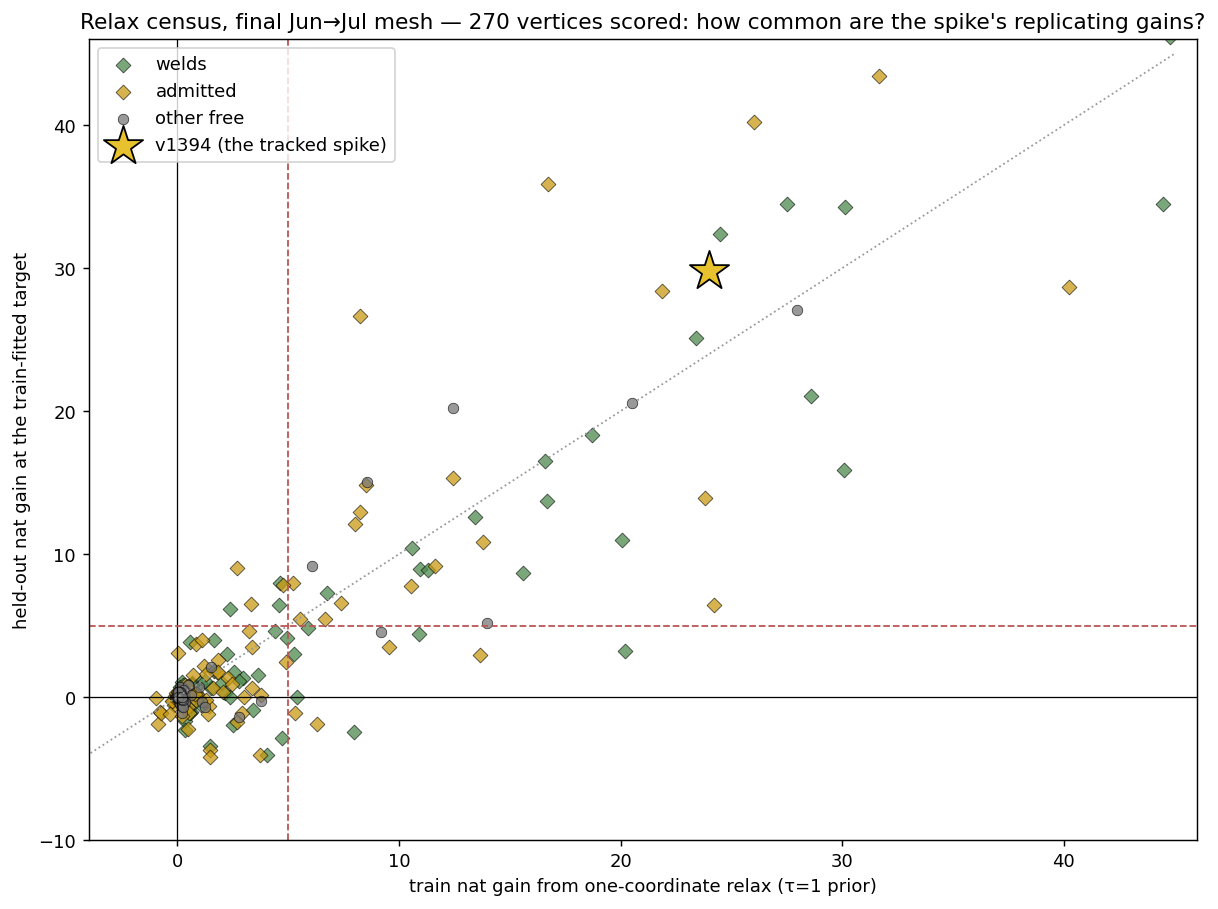
\includegraphics[width=0.8\textwidth]{relax_census_final.png}
\caption{Relax census on the final mesh: train versus held-out nat gain of
each vertex's one-coordinate relaxed fit. The replicating extreme class is
rare and clustered; the tracked vertex is the star.}
\label{fig:aug6-census}
\end{figure}

\paragraph{The two-currency principle (\textsc{measured}).} The diffuse class
is an artifact of scoring in the wrong currency. The relax criterion used the
law-\emph{marginal} likelihood; the solver ships the \emph{conditional}
surface; logit-normal attenuation puts the marginal-ML location
$\approx\frac12\sigma^2$ lower everywhere. Jointly refitting all 30 vertices
with $>20$ train nats (15 of them welds) executes this recalibration on 71\%
of the book and grades oppositely under the two currencies: held-out
deviance $2.794\to3.516$ (disaster) while held-out mixture NLL
$1.697\to1.644$ (the largest single improvement of the session). Pricing the
convexity into the prediction ($\bar p=\mathbb E[\mathrm{expit}(\eta+u)]$)
recovers only 0.11 of the 0.72 deviance gap: convexity is $\approx$15\% of
the wedge; the residual is the heavy-tail marginal acting as a \emph{robust
location estimator} (pulled toward the median pool) while mean prediction
needs the exposure-weighted mean --- i.e., the law books persistent fast
subpopulations as exchangeable tail noise, and the residual is the measured
prediction-space price of that misspecification. Consequences: the release
objective must be stated in the conditional/working currency for the
deployment target; the marginal surface-law fixed point is a research object
for distributional consumers; and $\mathrm{dev}(\bar p)$ joins the toolkit as
a \emph{currency detector} (the sign of $\mathrm{dev}-\mathrm{dev}(\bar p)$
identifies which optimum a surface occupies).

\paragraph{Three-currency scoreboard (\textsc{measured}, held-out,
June$\to$July).}

\begin{center}
\begin{tabular}{lccc}
\hline
surface & dev & dev$(\bar p)$ & mixture NLL\\
\hline
shipped & 2.7936 & 2.8347 & 1.69734\\
5-vertex local release & 2.7890 & 2.8297 & 1.69544\\
sharp-class release (19v, ad-hoc cut) & 2.7748 & 2.8013 & 1.67916\\
bulk $>$20-nat refit (30v) & 3.5155 & 3.4024 & 1.64405\\
hierarchical-$\tau$, marginal duals (128v) & 4.1713 & 4.0371 & 1.63238\\
hierarchical-$\tau$, conditional duals (66v) & \textbf{2.7355} & \textbf{2.7694} & 1.68570\\
\hline
\end{tabular}
\end{center}

The sharp-class release is the first intervention of the session to improve
all three currencies simultaneously; the conditional-dual hierarchical-$\tau$
release (below) then triples its deviance gain. Both carry mild selection
tint (held-out-informed cuts) and await fresh-seed confirmation.

\subsection{Stuckness, the ladder, and the hierarchical trust layer}
\label{sec:aug6-ladder}

\paragraph{Why geometry sticks (\textsc{measured} taxonomy).} Classifying the
19 sharp sites by mechanism (constrained descendants; trust and stiffness;
whether the law-GLS exact refit moves them): 5 are welds themselves; 6 are
closure-coupled free vertices (two rooms); 6 are \emph{soft-welded} free
vertices; 1--2 are temper-priced or joint-direction (valley) cases. The soft
welds are the discovery: $\lambda_v=10^8$ \emph{uniformly} across all 49
depth-8/9 admissions ($\lambda\sigma^2\sim10^{10\text{--}11}$, $T=0$,
rendered surpluses $\approx0$), against $\lambda\sim10^{-4}$ at depths
$\le7$: the fitted ladder is binary, free through depth 7 and welded from
depth 8. The clearest victim (v1599, depth 8) has $\sigma^2=7.3$
centilogit$^2$ --- excellent information --- and is pinned anyway. Bug lead:
with \texttt{DMESH\_TAU\_FLOOR\_LOGIT\_SD=0.005} the floor implies
$\lambda\le4$; depth 10 shows exactly $\lambda=4$ (floor working) while
depths 8--9 show $10^8$ (floor bypassed; sentinel or defect --- source read
queued). Unifying statement: evidence accumulates in nodal directions,
stiffness is levied in hierarchical ones; hard welds ($\lambda=\infty$), the
ladder's wholesale welds ($\lambda\to10^8$), and closure-coupled parents are
one Lagrangian phenomenon, and the principled repair is to make every
stiffness priceable by a dual (the whitened, conditional-currency,
footprint-aggregated score) with release and re-weld transitions under the
certification budget.

\paragraph{Hierarchical $\tau$, first working version (\textsc{measured}).}
A per-tier two-groups EM on the relax duals (tiers: free $\le d7$, free
$d8{+}$, welds; statistic: log train nats per ring pool; slab requires
posterior $>0.5$ and positive held-out gain), followed by a joint local
release of the slab. Fed \emph{marginal}-currency duals the EM selects 128
vertices (the attenuation field is a real nonzero signal in that currency)
and produces the worst deviance of the session (4.1713). Fed
\emph{conditional}-currency duals (plain binomial ring likelihood) it selects
66 vertices --- the corridor knob in, the diffuse giants out, 57 sites beyond
the ad-hoc sharp cut --- and produces the session's best surface on both
deviance currencies (table above). Same prior, same release machinery; only
the dual's currency changed. Caveats: the shallow-tier mixture separation is
weak (slab mean 0.006 nats/pool; near the two-cluster degeneracy),
posterior-threshold sensitivity and fresh-seed confirmation are required.

\paragraph{EB shrinkage, conceptual audit (\textsc{design}).} What is right:
the parent-interpolation null and per-scale variance decay. Four structural
defects, each with a session exhibit: (1) depth is the wrong exchangeability
unit (one $\tau$ spans K$_{\mathrm{eff}}$ 0.01 corridors and K$_{\mathrm{eff}}$
100 workhorses: the wholesale weld and the weak-plane self-licensing are the
two failure directions of the same choice); (2) the learning signal is
corrupted (fitted, entangled coefficients teach the ladder the solver's
ringing; gate truncation; working-binomial noise denominators understate by
2--3$\times$, and understated noise means overstated signal variance exactly
where noise is worst); (3) the gate and the ladder are two disconnected
inferences on the same hypothesis --- 49 of 118 gate-admitted coefficients
carry $\lambda=10^8$, admitted by one organ and welded by the other; the
correct object is a single spike-and-slab posterior per cell whose slab
probability \emph{is} the admission quantity and whose slab variance
\emph{is} the shrinkage; (4) the application point: compound-loss optimality
for coefficients is not optimality for the field; shrinkage enters only
through $\Lambda$ in the joint conditional-currency solve. Target design, all
components individually validated this session: spike-and-slab per
(depth $\times$ evidence-geometry) cell, fitted by g-modeling on whitened
coefficients or data-side duals over the full candidate ensemble including
refusals, sandwich-honest denominators, unified with the gate, applied
in-loop, re-priced on design-changing events. The measured bar for the
in-loop implementation is the conditional-dual release's 2.7355.

\subsection{Session open-item delta}\label{sec:aug6-open}

New or re-ranked relative to Section~\ref{sec:discussion}: (1) the release
rule and redistricting review (in-loop; conditional currency; e-BH budget);
(2) the \texttt{TAU\_FLOOR} bypass at depths 8--9 (bug read); (3) in-loop
two-groups $\Lambda$ with the marginal Newton, bar 2.7355; (4) sandwich se
inside the exact scorer (unchanged, still first); (5) fresh-seed confirmation
of the sharp-class and conditional-slab releases; (6) the 11-site weld docket
with pre-registered targets, and the 3 train-only firings as the block-null
test set; (7) exact-age dummies or anisotropic refinement at the issuance
boundary (unchanged); (8) the marginal surface-law fixed point as a
research note for distributional consumers.


% ---------------------------------------------------------------------------
% August 12 session: the shrinkage ladder, the exchangeability principle, the
% two-currency verdict, and the in-loop negative result.  Inserted 2026-08-12.
% ---------------------------------------------------------------------------
\section{August 12 session: the shrinkage ladder, the exchangeability principle, and the two-currency verdict}\label{sec:aug12}

This session works the empirical-Bayes conceptual audit of
Section~\ref{sec:aug6-ladder} as an implementation program. It resolves the
queued \texttt{TAU\_FLOOR} bug lead; builds and measures a family of
prior-variance estimators against audit defects~1 (depth is the wrong
exchangeability unit) and~2 (the learning signal is corrupted); reaches a
clean two-currency verdict on what re-shrinkage can and cannot buy; and
returns a decisive negative result on the naive route to defect~3 (unify the
gate and the ladder) that converts the spike-and-slab target from a
preference into a requirement. Status labels as before: \textsc{measured},
\textsc{design}, \textsc{retracted}. Unless noted, numbers are held-out on the
June 2026 SMM design (33{,}740 pools, one-law config, seeds 7 and 101--110),
scored in \emph{two currencies}: mean binomial deviance per pool (the
conditional, point-prediction currency) and held-out mixture NLL evaluated by
reference against one fixed law (the marginal currency of
Section~\ref{sec:aug6-release}).

\subsection{The wholesale weld, resolved}\label{sec:aug12-floor}

\textsc{Measured.} The August 6 bug lead --- $\lambda_v=10^8$ across all
depth-8/9 admissions against a floor-implied cap of $4$, with depth 10 showing
the cap working --- is a defect in the final post-selection re-shrinkage pass
(\texttt{DMESH\_FINAL\_RESHRINK}), not the ladder or a sentinel. The mechanism:
$\lambda_v=1/\texttt{tau\_for\_depth}(d)$ and every $\tau$ read is floored at
\texttt{tau\_floor\_sq}, so at the documented
\texttt{DMESH\_TAU\_FLOOR\_LOGIT\_SD}=0.005 the floor caps $\lambda_v\le4$. The
reshrink pass re-estimated $\tau$ per depth from raw surpluses and then
\emph{overwrote the floor itself} (\texttt{tau\_floor\_sq}$\leftarrow10^{-8}$),
opening two weld channels: (i) a depth whose truncation-corrected $\chi^2$ sits
below its selection-inflated null gives $\tau=0$, floored at $10^{-8}$, i.e.\
$\lambda_v=10^8$ for every admitted coefficient at that depth in one stroke;
(ii) the lowered floor outlives the pass, so the closing height sweeps'
in-loop $\tau$ recomputes weld depths the pass itself read as positive. The
``$d10$ shows the floor working'' reading is corrected: it was the
improvement-only clamp passing through an already-floored in-loop value, not
the floor holding at read time. \textbf{Fix}: the reshrink keeps its honest
re-estimation but no longer lowers the floor;
\texttt{DMESH\_RESHRINK\_NO\_FLOOR} restores the historical behaviour
(bit-verified against a pre-fix build). On the SMM design the floor bound on 8
of 11 seeds; held-out deviance improves $1.1661\to1.1552$ in mean, the worst
case a full depth-6 workhorse tier (40 coefficients, median $|$surplus$|$ 43
centilogits) welded wholesale and recovered $1.292\to1.205$ (seed 103).
Ledger entry~(12).

\subsection{Depth is the wrong exchangeability unit, and $K_{\mathrm{eff}}$ is
not the right one either}\label{sec:aug12-ladder}

Audit defect~1 asks for the prior grouping. A family of estimators, all inside
the reshrink pass and selected by \texttt{DMESH\_RESHRINK\_LADDER}, was built
and measured: \texttt{cells} (split each depth at a $K_{\mathrm{eff}}$
threshold), \texttt{keffcont} (threshold-free per-vertex
$\tau_d/(1+r)$, $r=\mathrm{Var}_{\mathrm{pool}}/\mathrm{Var}_{\mathrm{bin}}$
the same pool-effect inflation the gate prices), \texttt{eb}
(selection-corrected marginal maximum likelihood for $\tau$ with a hierarchical
borrow toward a global fit, replacing the ad-hoc $4^{-\Delta d}$ decay),
\texttt{ebscale} (a single smooth per-scale law $\tau(d)=\tau_0\rho^d$ as the
hyperprior mean), and \texttt{twogroups} (a per-depth spike-and-slab EM). The
$K_{\mathrm{eff}}$ deflation of $r$ uses the one-law per-pool variance, so the
count that indexes a cell is the effective number of \emph{independent
pool-level} observations, not raw loan mass.

\paragraph{The exchangeability principle (\textsc{measured} conclusion).}
$K_{\mathrm{eff}}$ measures the \emph{strength of the data support}, not the
signal. The amount of signal is exchangeable over scale even though
$K_{\mathrm{eff}}$ is not, so the prior variance must be exchangeable over
signal coordinates (scale/depth) and $K_{\mathrm{eff}}$ must be factored
through the \emph{likelihood} --- the per-coefficient posterior shrink
$\tau/(\tau+v_i)$ --- never used to index the prior. Three measurements
confirm it: (a) \texttt{ebcell}, which puts $K_{\mathrm{eff}}$ \emph{into} the
prior grouping, does not improve on \texttt{eb}; (b) \texttt{ebscale}, whose
prior sees only scale, matches \texttt{eb} in mean with the \emph{tightest
cross-seed spread} of any arm (sd $0.036$), i.e.\ the scale-exchangeable prior
buys stability by refusing to chase per-depth sampling noise; (c)
\texttt{keffcont}'s $\tau_d/(1+r)$ is algebraically one exchangeable $\tau_d$
under the law-aware posterior precision $x^\top x/(1+r)$ --- $K_{\mathrm{eff}}$
in the likelihood, exactly as prescribed. \texttt{twogroups} over-shrinks
(fit on the admitted set only, so it cannot estimate the null fraction) and is
not adopted.

\begin{center}
\begin{tabular}{lcc}
\hline
reshrink estimator & held-out dev/pool & sd across seeds\\
\hline
off (no reshrink)              & 1.1545 & 0.039\\
depth (per-depth moment)       & 1.1552 & 0.039\\
cells ($K_{\mathrm{eff}}$ split)& 1.1595 & 0.033\\
keffcont (law-aware posterior) & 1.1534 & 0.038\\
\texttt{eb} (MMLE + borrow)    & \textbf{1.1502} & 0.038\\
ebscale (scale prior, clamped) & 1.1508 & \textbf{0.036}\\
twogroups (per-depth slab)     & 1.1671 & 0.034\\
ebscale + honest $v_i$, free   & 1.1421 & 0.041\\
\hline
\end{tabular}
\end{center}

The ranking is monotone in statistical principle: law-aware counting beats raw,
threshold-free beats threshold, and MMLE with hierarchical borrowing beats
method-of-moments. \texttt{eb} is the recommended reshrink estimator where the
point-prediction currency is the target: it wins or ties the shipped
per-depth default on 10 of 11 seeds with no catastrophic seed.

\subsection{Honest per-pool variance}\label{sec:aug12-vi}

Audit defect~2 (working-binomial noise denominators understate by $2$--$3\times$
where pool effects dominate). Once the prior is blind to $K_{\mathrm{eff}}$,
every measurement fact rides on $v_i$, so $v_i$ must be honest. The shipped
one-law prices pool-effect variance in four size strata --- an $8.5\times$ step
at $n_0=512$. \textsc{Measured}: replacing the step with a smooth log-log
interpolation of the stratum variances in pool size (a pure size covariate, no
conditioning on the pool's own residual, so no surface-error absorption of the
kind that inflated the retracted heavy-tail law), applied fleet-wide so it
feeds both the gate null and the reshrink $r$, is a real but modest win:
$+0.0014$ on \texttt{eb}, $+0.0065$ alongside the scale prior --- more where
the prior is thinner and $v_i$ carries more weight, exactly as the
factorisation predicts. This is only the crudest de-bucketing; the per-pool
predictive $\mathbb E[u^2\mid\text{data}]$ (which stays large for small pools,
where the posterior \emph{mean} would wrongly read them clean) is the deeper
version and is deferred.

\subsection{The two-currency verdict}\label{sec:aug12-currency}

\textsc{Measured}, and the load-bearing result of the session. Every estimator
above improves the conditional (deviance) currency and \emph{washes out in the
marginal (NLL)}. The reshrink pass edits coefficient heights at frozen
topology; it cannot change which vertices were admitted, and the pool-effect
law absorbs a surface change of this magnitude once the pool effect is
integrated out. On the full April Ginnie design (120{,}595 pools) all nine
estimators give held-out mixture NLL in $[2.5963,2.5965]$ --- a spread of
$2\times10^{-4}$ --- while held-out deviance moves $6.5803\to6.5577$. On the
SMM design the NLL spread is $\approx0.004$ against a deviance spread of
$\approx0.02$, and plain no-reshrink (NLL $0.9074$) ties or beats several
reshrink arms; only the aggressive-plus-honest-$v_i$ combination gets under it
($0.9059$). Stated in the two-currency language of
Section~\ref{sec:aug6-release}: the reshrink ladder is a point-prediction
improvement, not a distributional one. Moving the marginal currency requires
changing \emph{which coefficients are admitted}, not re-shrinking the admitted
set.

\subsection{Admission is not reachable by a prior swap}\label{sec:aug12-admission}

Audit defect~3 (the gate and the ladder are two inferences on one hypothesis).
The in-loop prior does reach admission: the candidate exact gain is scored
against prior precision $1/\tau$, so $\tau$ sets the admission bar, not only the
shrinkage. Moving the \texttt{eb} estimator into the in-loop
\texttt{recompute\_tau\_sq} (\texttt{DMESH\_INLOOP\_EB}) therefore puts it into
the gate. \textsc{Measured} (SMM seed 7): it \emph{over-admits} --- mesh
$348\to454$ vertices ($+30\%$) --- and worsens both currencies, deviance
$1.189\to1.435$ and NLL $0.9074\to0.9387$. This reproduces the
shrink\,$\to$\,residual\,$\to$\,re-admission spiral the reshrink architecture
exists to avoid: the hierarchical borrow relaxes the sparse-tier prior, the
relaxed prior raises the admission gain, the newly admitted coefficients absorb
residual and expose more apparent signal, and the loop amplifies. The in-loop
moment's conservatism is load-bearing, and swapping in the honest prior
in-loop removes it.

The lesson is structural: admission cannot be coupled to shrinkage through an
\emph{unregularised} prior. The audit's own target design already carries the
missing regulariser --- a single spike-and-slab posterior per
(scale $\times$ evidence-geometry) cell, fitted by g-modelling on the
\emph{full candidate ensemble including refusals}, whose slab probability
\emph{is} the admission quantity and whose slab variance \emph{is} the
shrinkage. There the null fraction $\pi$, anchored by the refused candidates,
controls admission stringency directly, so admission and shrinkage move
together without the tug of war a bare in-loop $\tau$ swap sets up. The
negative result identifies $\pi$ --- the quantity a shrinkage estimator alone
never sees --- as precisely what the naive route lacks.

\subsection{Session open-item delta}\label{sec:aug12-open}

New or re-ranked relative to Section~\ref{sec:discussion}: (1) \texttt{eb} is
the recommended reshrink estimator on the one-law config for the
point-prediction currency (robust, $+0.004$ deviance, 10/11 seeds); the ladder
itself is settled and the remaining ladder work is the EB $\tau$ multiplier
below. (2) The EB $\tau$ multiplier: replace the improvement-only clamp
$\min(\tau_{\mathrm{reshrink}},\tau_{\mathrm{loop}})$ with a continuous factor
on the loop $\tau$, estimated by marginal likelihood and regularised toward $1$,
so the data --- not a kink --- decides how far to move off the in-loop
regularisation; the aggressive gains ($\texttt{ebscale\_free}$, seed-104 tail)
are otherwise entangled with lifting the clamp. (3) The unified spike-and-slab
on the full candidate ensemble is \emph{the} route to the marginal currency;
the in-loop negative result upgrades it from a design preference to a
requirement, with $\pi$ the identified missing piece. (4) Per-pool predictive
$v_i=\mathbb E[u^2\mid\text{data}]$, replacing the size-only de-bucketing.


\section{Discussion}\label{sec:discussion}

The open items of the program, consolidated and current as of August 5, 2026.
This list supersedes the per-section lists; historical item statuses live in the
appendices and the ledger.

\begin{enumerate}[leftmargin=2em,itemsep=3pt]
\item \textbf{Certification.} The formal exact-score (B3) transfer remains open.
The practical route is cross-fitted e-BH over held-out directional
log-likelihood gains --- finite-sample FDR at level $q$ under arbitrary
candidate dependence, conditional on the construction sample --- with
enumeration-validated double-saddlepoint conditional $p$-values as the
per-candidate evidence in the sparse-count regime. The corrected null datasets
and the ten-mask harness of Section~\ref{sec:aug5} are the predeclared
falsification suite; the certified object becomes ``out-of-sample-replicable
structure,'' which is the claim a validator can audit.
\item \textbf{Admission stability.} Measured and decomposed
(Section~\ref{sec:aug5-churn}): $\approx79\%$ of the evidence-weighted churn
is the power floor a correct gate would exhibit ($J_W$ benchmark $0.51$, not
$1.0$); the excess is one-fifth path dependence (ancestor availability,
removable by a union-topology two-stage pass) and a misspecification residual
concentrated in a $\sim5\%$ boundary-riding tail at $6\times$ the floor,
with issuer-block correlation the leading suspect. Remedies now rank:
union-topology stability selection with published per-vertex selection
frequencies $\pi_v$; issuer-block resampling in the null; a graduated
(precision-scaled) sub-threshold tier for what the floor itself cannot
certify. In-loop marginal fitting remains the fit-side complement; the
balanced-seed bar for any of these is mixture NLL $0.92201$.
\item \textbf{Gate mechanics.} Whether \texttt{gate\_k4} enters the released
pricing; depth-aware support rules; the double-saddlepoint tail computation as
the permutation logic's repair where moment standardization failed.
\item \textbf{The law.} Cross-split confirmation of the converged SMM pool law,
estimated to date on one split's training half.
\item \textbf{Data.} The two-month Ginnie panel: the identifiability keystone,
the only route to $\sigma_a^2$ proper, and the first innovation observation of
the temporal layer. Before any option-valuation use, split maturity and buyout
removals from voluntary payoffs (the amortization-endgame island of
Section~\ref{sec:aug5}) or carry original term as a known covariate. The
Fannie/Freddie historical performance datasets are the out-of-population
replication sets.
\item \textbf{Temporal layer.} Fix and pre-register the test dictionary before
any dynamics are fit (Section~\ref{sec:aug5-temporal}); the null model is pure
transport in vintage coordinates.
\item \textbf{Process.} Pin Section~\ref{sec:current}'s stated defaults to
\texttt{run\_config} by a build-time regression test, so the specification
cannot silently lag the code the way the \texttt{DMESH\_SIGMA0\_MIN} default
lagged the documented central-matching constraint.
\end{enumerate}

Where the program stands: the fitted system is self-consistent --- surface,
law, gate pricing, and null batteries derive from one converged pair on a
solver that cannot erupt --- its failures are located and bounded rather than
diffuse, and what remains is one theorem, one panel, and one in-loop
implementation. Many older figures remain single-split illustrations and are
labeled as legacy where their interpretation has changed.

\appendix
\section*{Appendices: the April-proxy-era evidence base}
The appendices preserve, unrewritten, the numerical, real-data, certification, and
forensic evidence of the April-proxy era together with the loan-level and tail-shape
theory developed against it. Every result here is a correct measurement of its era;
scales are not comparable to the June SMM numbers of Section~\ref{sec:aug5} (see the
datasets note on the state page), and superseded claims are listed in the ledger of
retractions at the front of the paper.

\section{Numerical evidence}\label{sec:numerics}
\label{sec:oracle}

The review notes, correctly, that no analogue of the
Binev--Dahmen--DeVore/Abramovich rate results is even conjectured here. This
section scopes what such a theorem would have to prove, with an honest
account of what the empirical study can and cannot establish.

The right decomposition separates mesh \emph{placement} from height
\emph{estimation}: at matched vertex count $N$, compare the interpolation
error of the true $f$ on (i) a reference topology built by a noiseless
greedy (projection-gain scoring, no gate, no shrinkage) and (ii) the
topology the gated pipeline selected from \emph{noisy} data; both under
the identical interpolation rule, so that only placement differs
(Figure~\ref{fig:oracle}). The result: the gated topology \emph{beats} the
greedy by a factor of $2$--$3$ at matched $N$ on both surfaces
(uniform: $5.4$ vs.\ $15.8$ weighted RMSE at $N\!\approx\!700$; chirp:
$20$ vs.\ $48$ at $N\!\approx\!925$). Since nothing can beat a genuine
near-optimal oracle, the correct reading is that batched projection-gain
greedy is a \emph{baseline}, not an upper benchmark: it is blind to NVB
closure costs (conformity bisections spend budget its indicator never
prices) and its batch admissions lose greedy fidelity. What the study
establishes is therefore a floor, cleared decisively: the gate's
noise-facing selection places vertices better than a natural noiseless
greedy. The upper benchmark the adaptivity conjecture needs; one-at-a-time
greedy with closure-aware error accounting; is specified and queued; the
conjecture itself would then read: the gated topology's interpolation error
at $N$ vertices is within a constant of that benchmark's, with the constant
degrading gracefully in the FDR target. On the chirp the gated topology's
error--$N$ slope is $\approx-0.7$ against the ideal $N^{-1}$ (two effective
budgets, one seed: indicative only).

Two methodological findings from constructing the study deserve record.
First, an unregularized least-squares fit on an adaptive mesh (the naive
oracle-with-fitting) is \emph{worse at more vertices}: fine vertices with
under-determined stars hold arbitrary heights between data points, invisible
to in-sample metrics and dominant in integrated ones; which is a
back-handed validation of the EB layer, since exactly this pathology is what
the parent-interpolation prior suppresses in the pipeline proper. Second,
the pure-interpolation error of the gated topology ($\approx5$ weighted RMSE
units on the uniform surface) is an order of magnitude below the noisy fit's
error ($\approx60$--$70$): at these information levels the fit is
estimation-noise dominated, so mesh-placement optimality is not the binding
constraint on accuracy; consistent with the cap-sweep finding that
coarser meshes can win.

\begin{figure}[h]
\centering
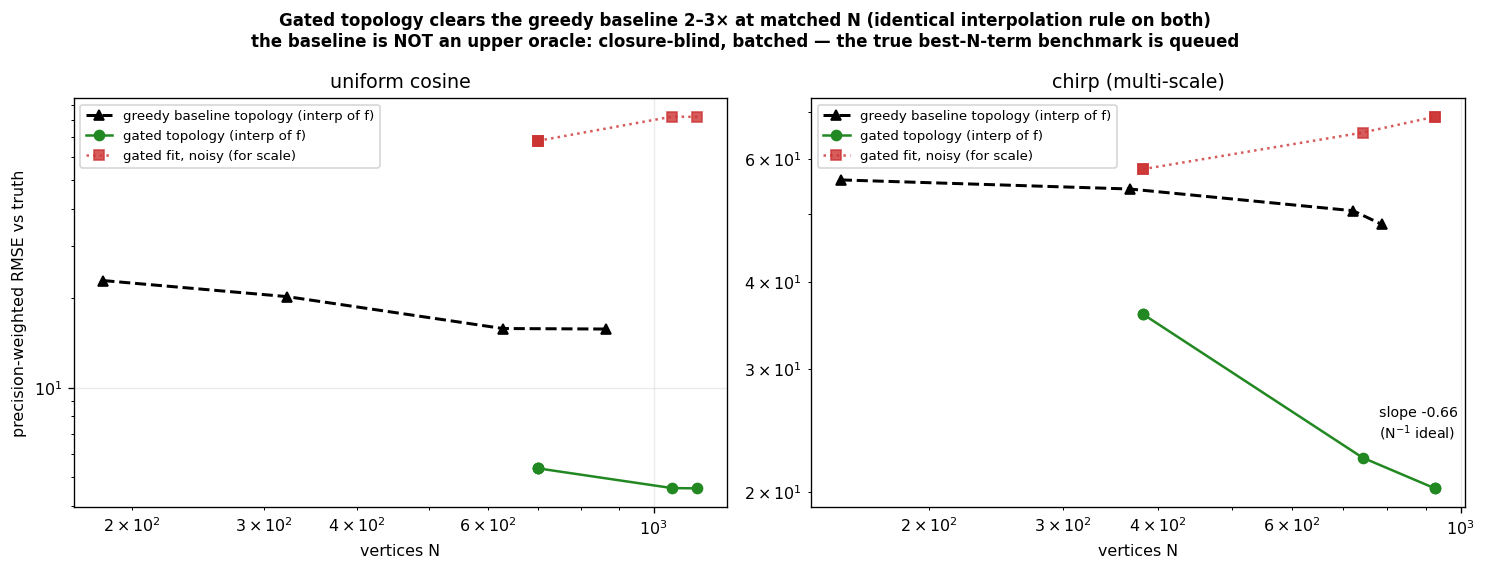
\includegraphics[width=\textwidth]{fig14_oracle_ratio.png}
\caption{Placement quality at matched $N$: interpolation of the true $f$ on
the gated topology (green) vs.\ a noiseless greedy baseline (black), with
the noisy fit (red) for scale. The gated topology clears the baseline by
$2$--$3\times$; the baseline is not an upper oracle (closure-blind,
batched), so no oracle \emph{ratio} is claimed; the closure-aware
benchmark is queued.}
\label{fig:oracle}
\end{figure}

\subsection{Gate calibration, attribution, and effective exposure}\label{sec:sims}


\begin{figure}[ht]
\centering
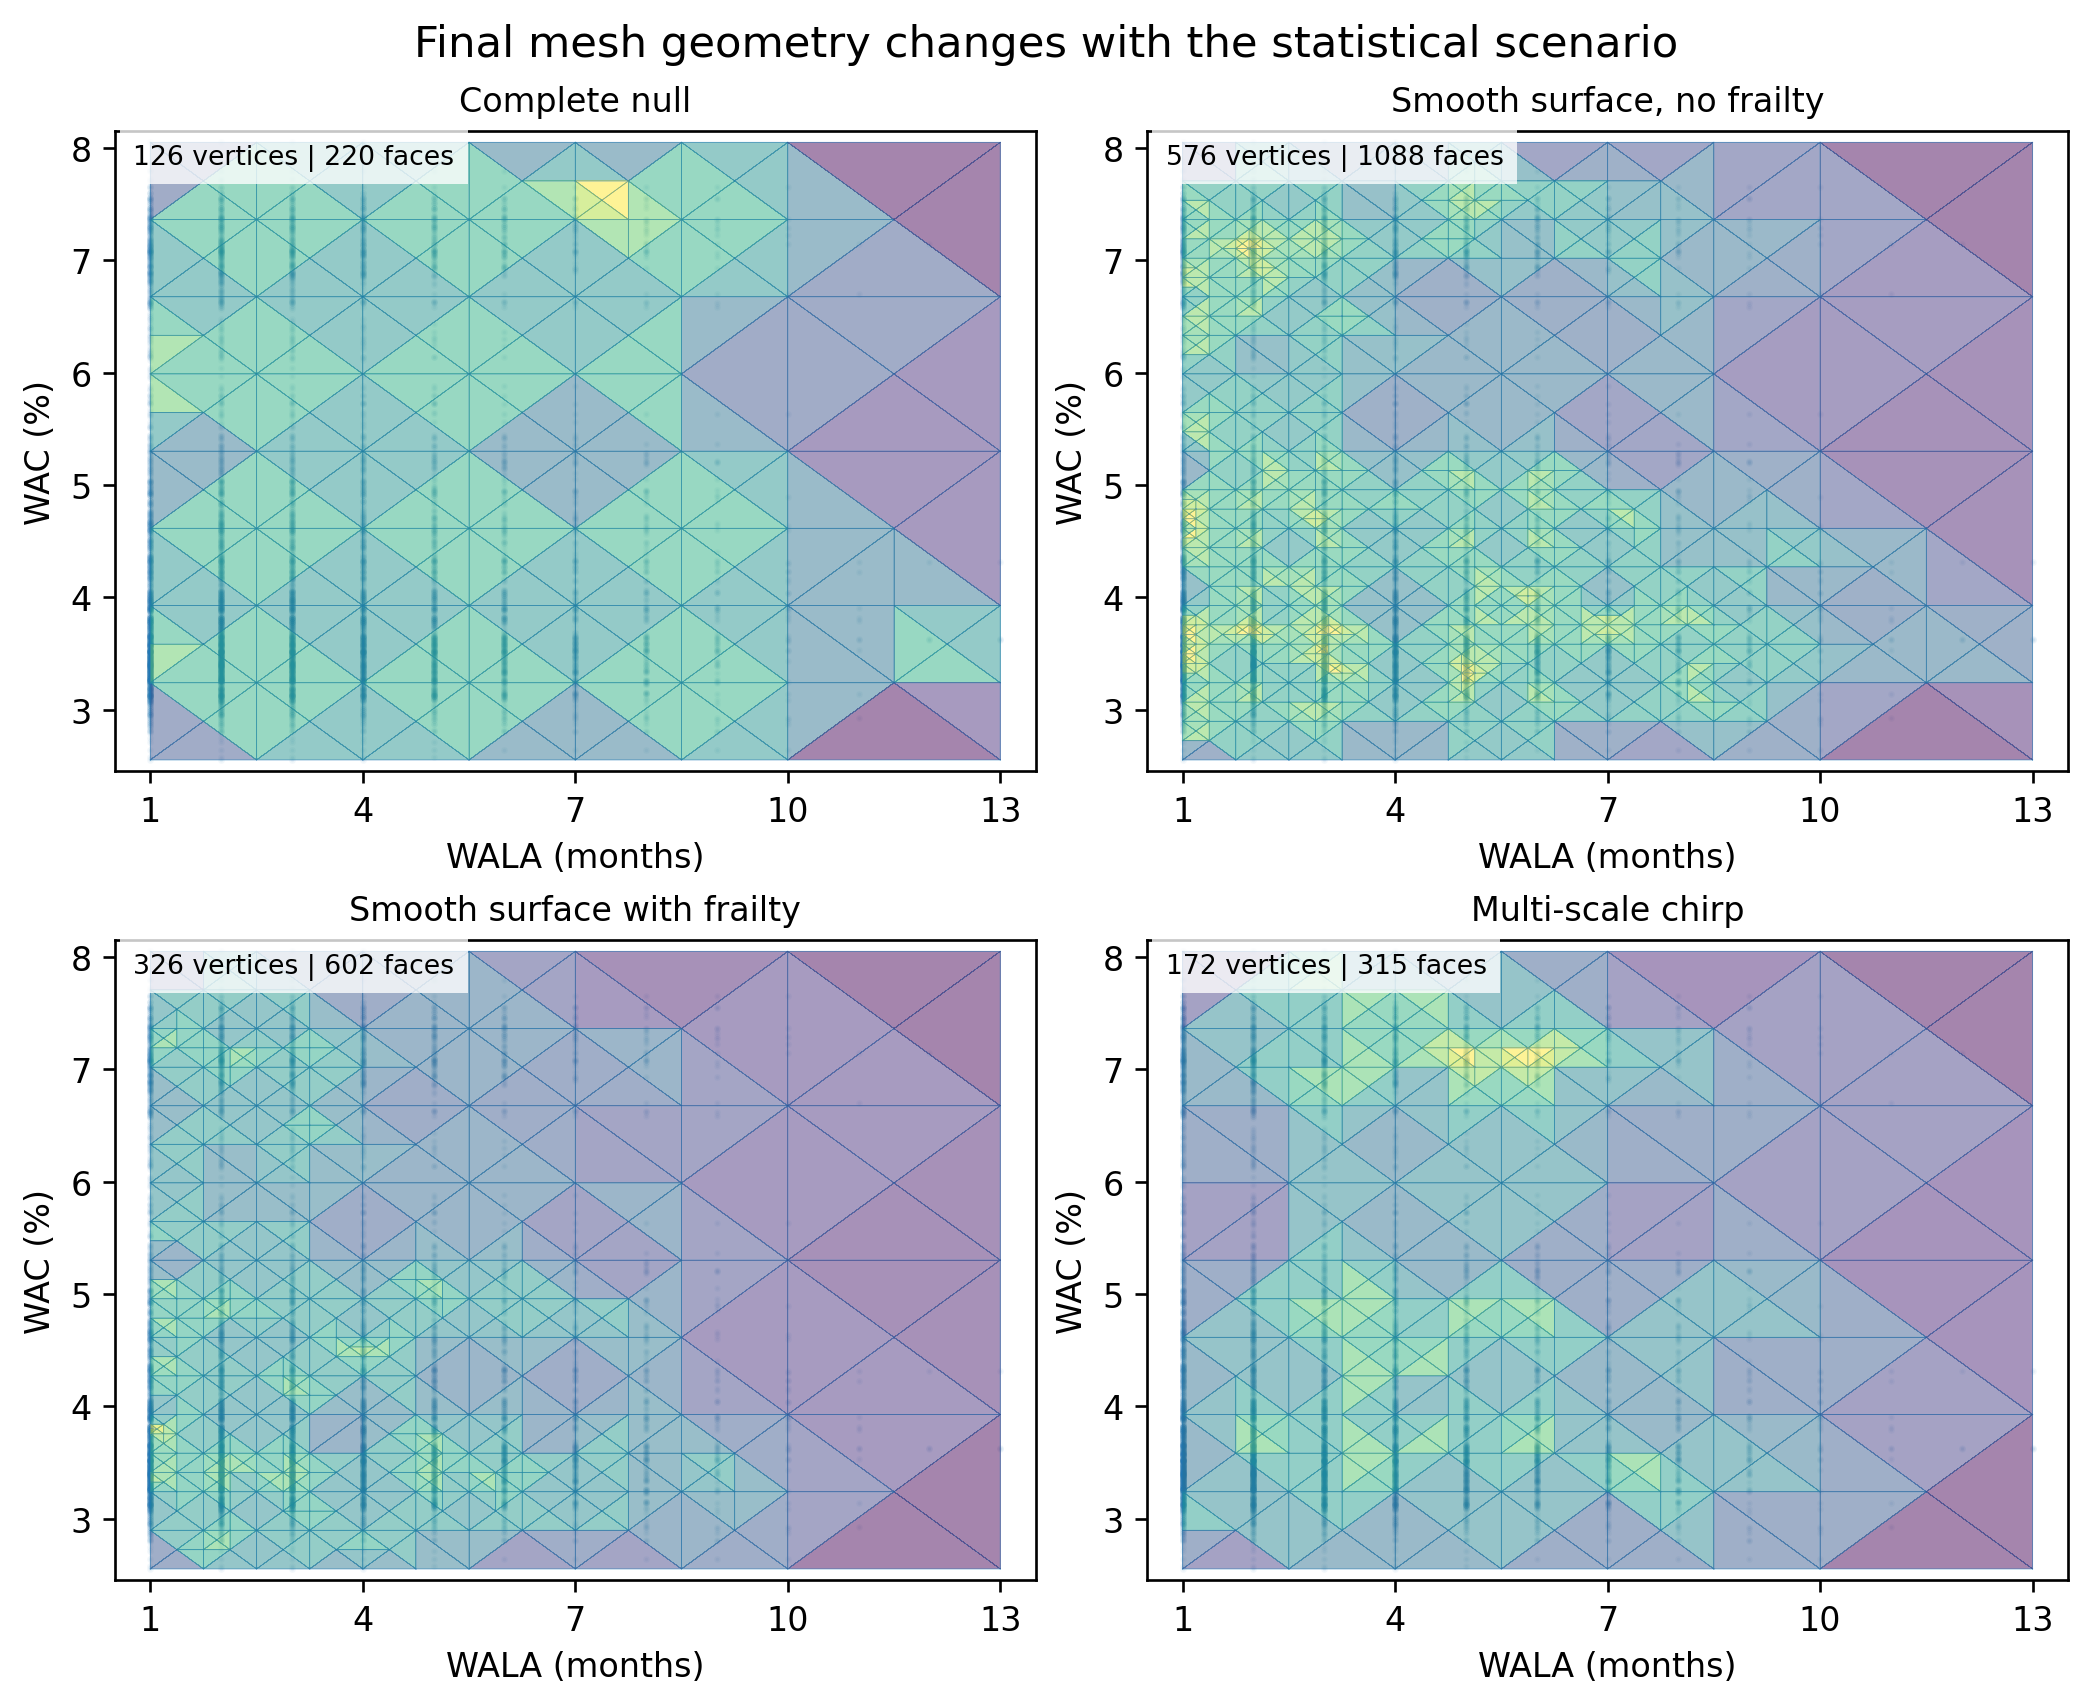
\includegraphics[width=0.88\textwidth]{fig21_mesh_scenario_gallery.png}
\caption{Final meshes for matched-support experiments. Face color records mean refinement depth. The complete null remains comparatively coarse; smooth signal induces coherent refinement along support; adding persistent pool variation changes the fitted uncertainty more than the broad geometry; and the chirp spends substantially more depth where the target oscillates rapidly.}
\label{fig:mesh-gallery}
\end{figure}

\begin{figure}[ht]
\centering
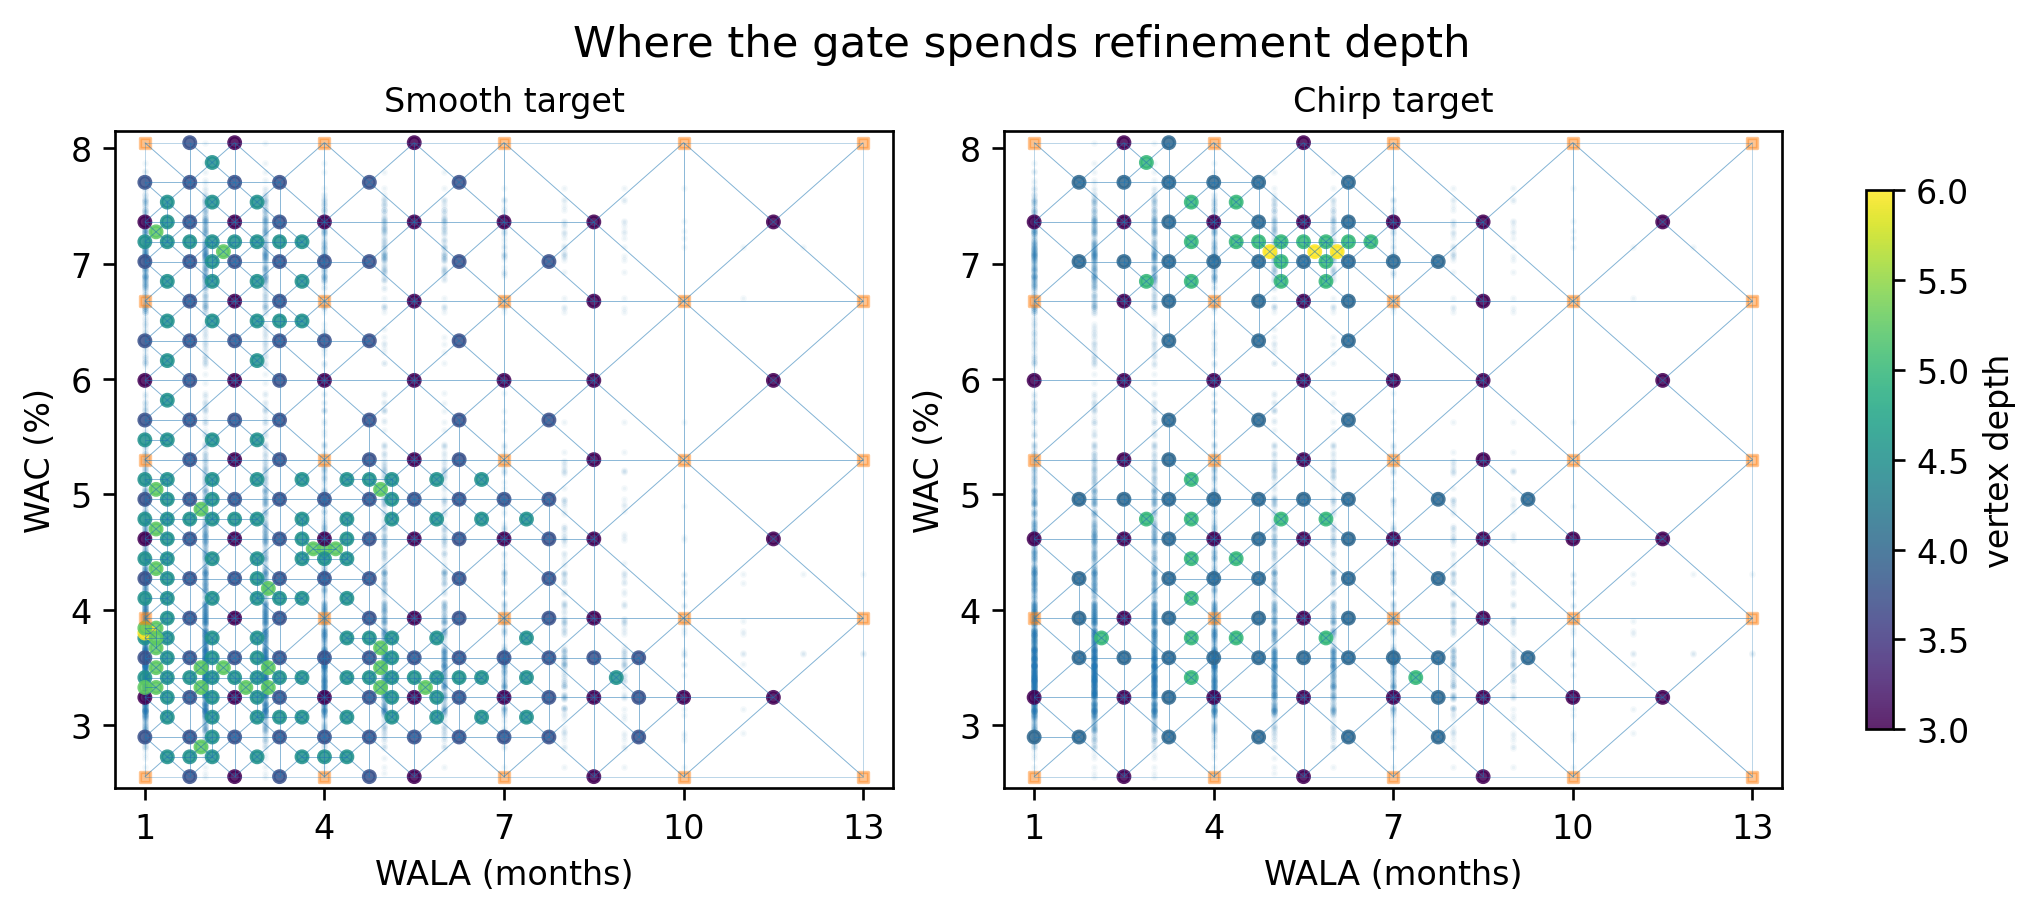
\includegraphics[width=0.88\textwidth]{fig23_admitted_vertex_depth.png}
\caption{Locations and depths of active nonstructural vertices in representative smooth and chirp runs. The smooth target distributes refinement broadly along supported cohort bands, whereas the chirp concentrates deep vertices in its fast-scale region. The plot links the statistical gate directly to the geometry it creates.}
\label{fig:vertex-depth}
\end{figure}

\begin{figure}[h]
\centering
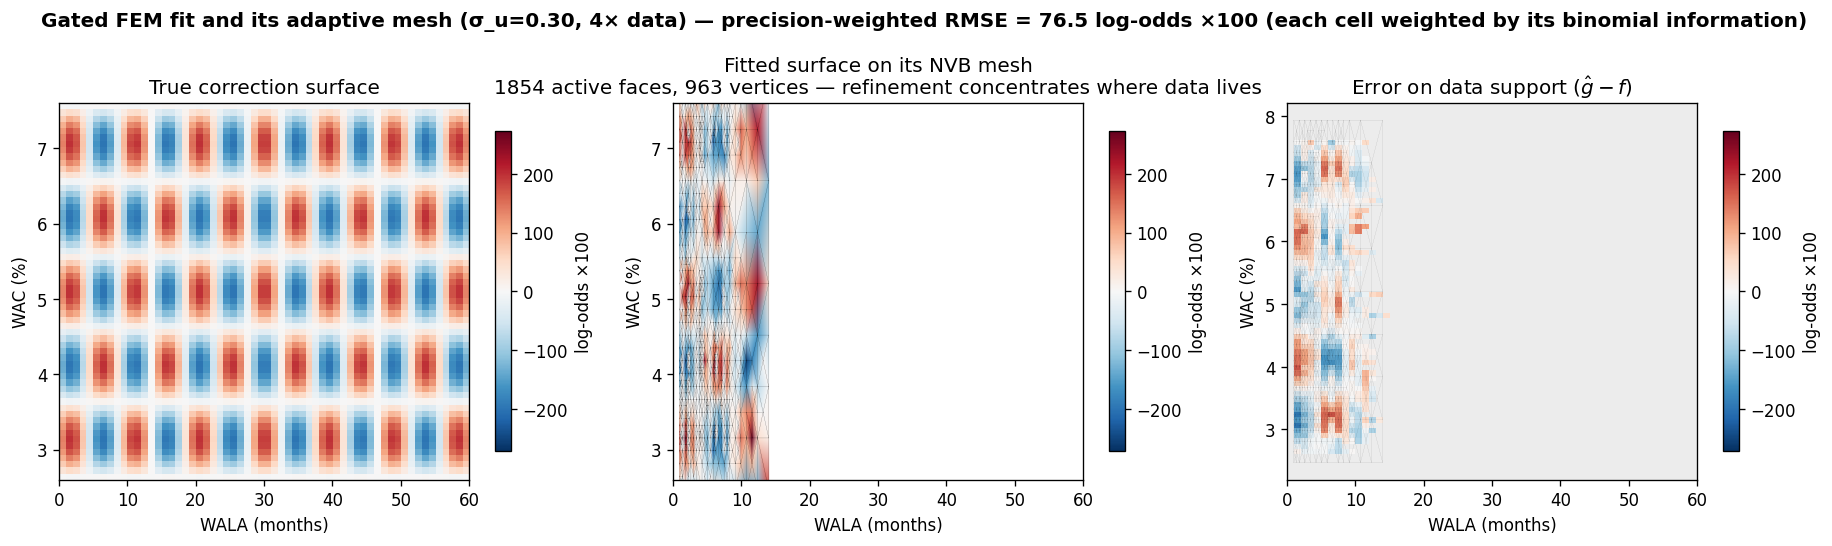
\includegraphics[width=\textwidth]{fig1_surface_mesh.png}
\caption{Uniform-cosine target ($\sigma_u=0.30$, $4\times$, 24 pts/face). True surface; fit on its NVB mesh (refinement concentrates on the data support, flat off-support by the zero-mean prior); error masked to support. The quoted precision-weighted RMSE weights each cell by its binomial information.}
\label{fig:surface}
\end{figure}


\begin{figure}[h]
\centering
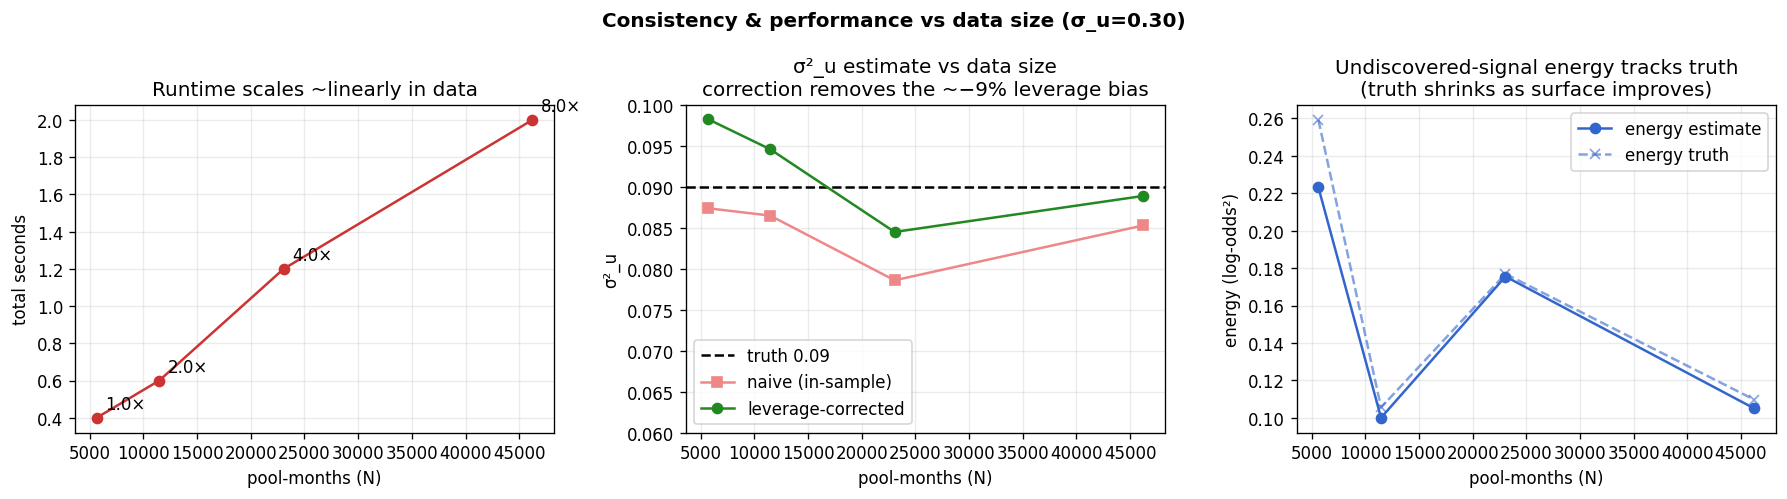
\includegraphics[width=\textwidth]{fig5_scaling.png}
\caption{Legacy scaling experiment (single seed per point; wiggles are sampling noise). Runtime is near-linear in $N$, and the leverage correction reduces the naive same-data bias. The earlier claim of an approximately constant $9\%$ correction is superseded by the current multi-seed frailty sweep in Figure~\ref{fig:current-reruns}, which finds increasing residual underestimation at high frailty.}
\label{fig:scaling}
\end{figure}


\begin{figure}[h]
\centering
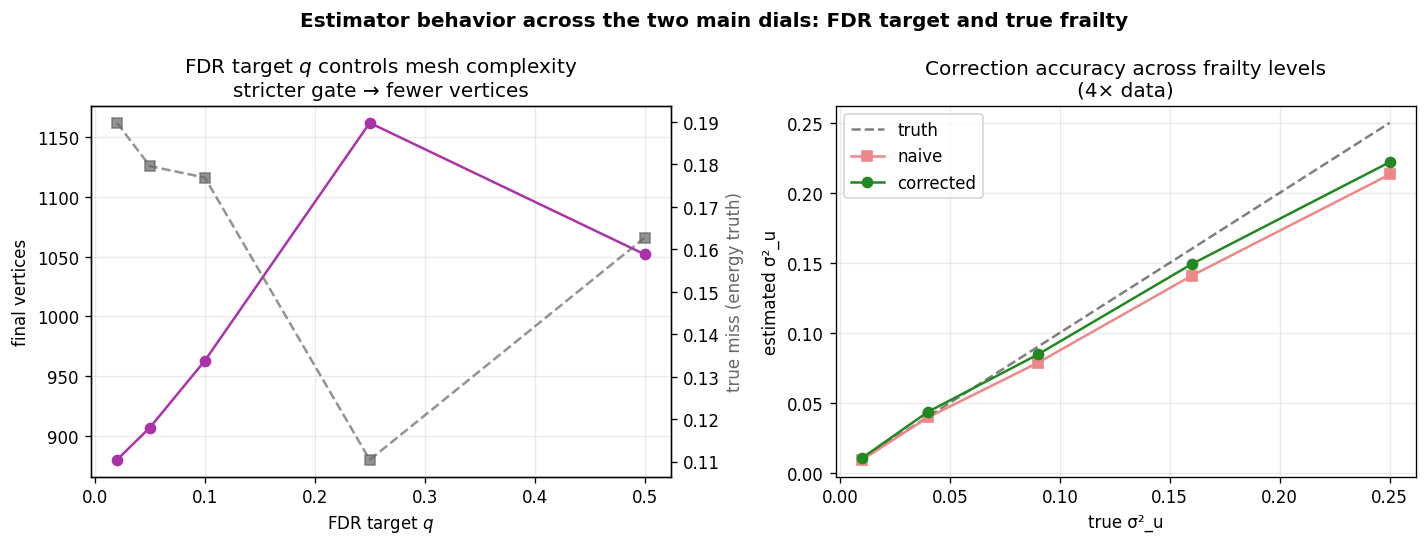
\includegraphics[width=\textwidth]{fig6_sweeps.png}
\caption{Legacy single-seed dial sweep. Left: the FDR target $q$ controls mesh complexity against detected miss. Right: naive vs.\ leverage-corrected $\hat\sigma_u^2$ across true frailty levels. The current five-seed reruns in Figure~\ref{fig:current-reruns} replace the old smooth U-curve interpretation and quantify the remaining high-frailty bias.}
\label{fig:sweeps}
\end{figure}

\begin{figure}[ht]
\centering
\begin{minipage}[t]{0.49\linewidth}
\centering
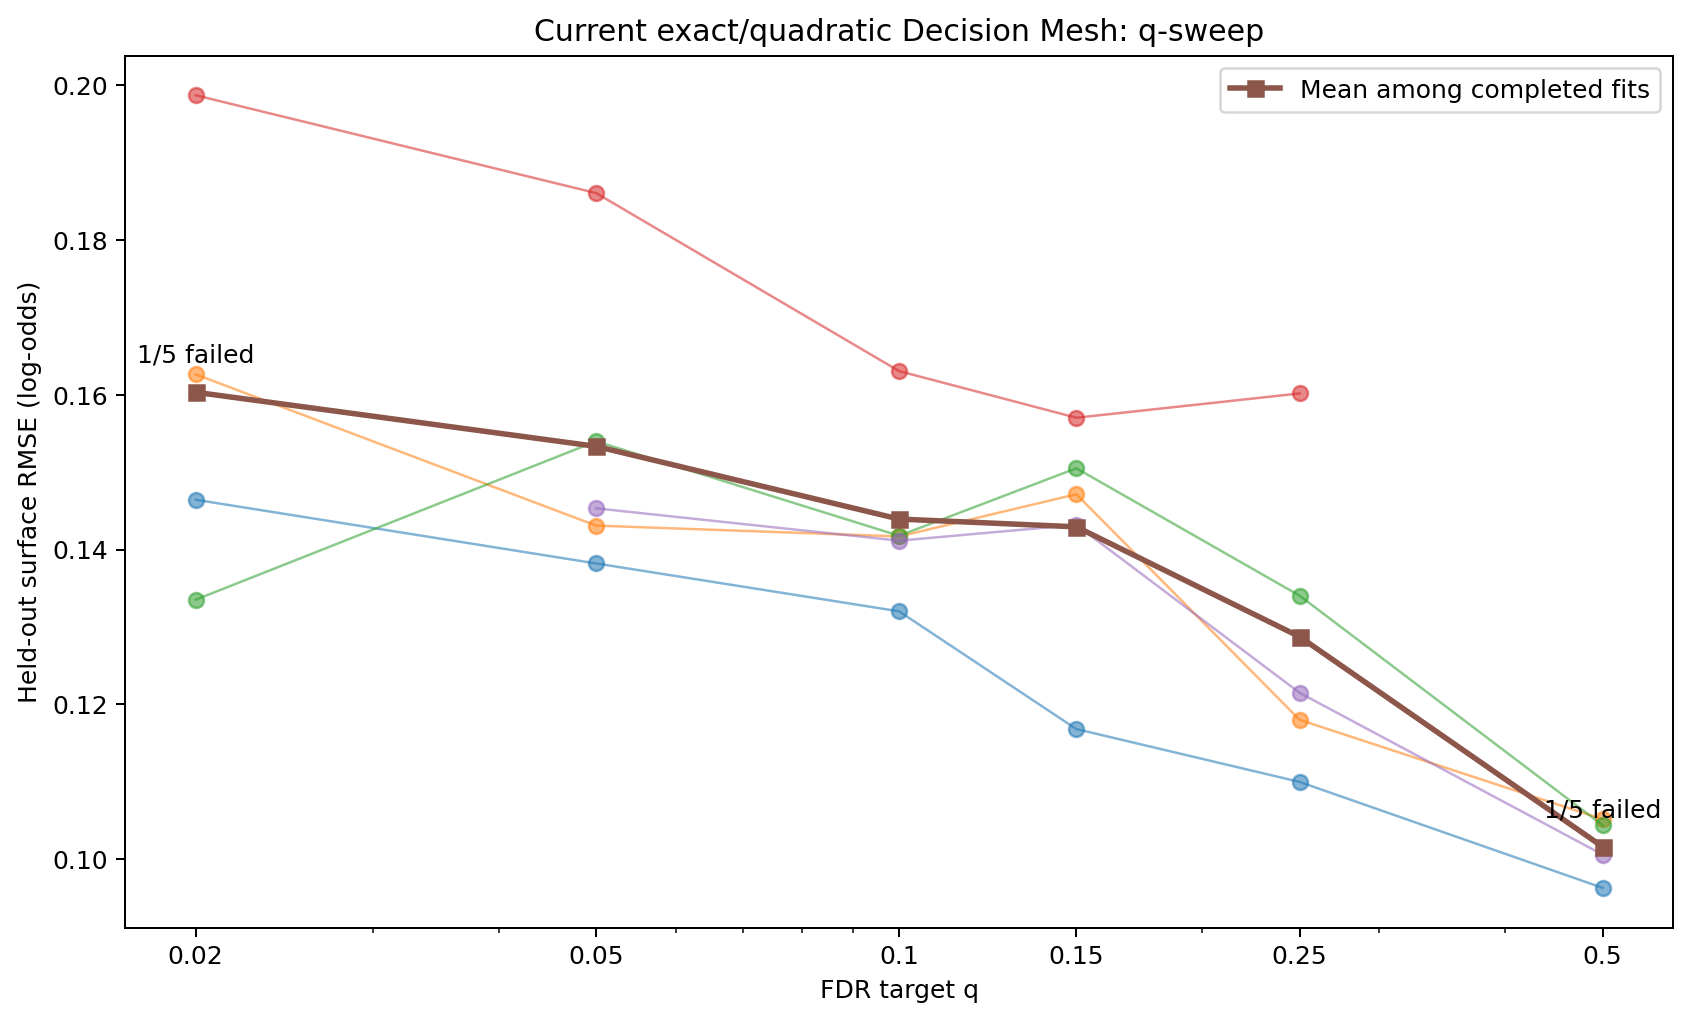
\includegraphics[width=\linewidth]{current_qsweep.png}
\end{minipage}\hfill
\begin{minipage}[t]{0.49\linewidth}
\centering
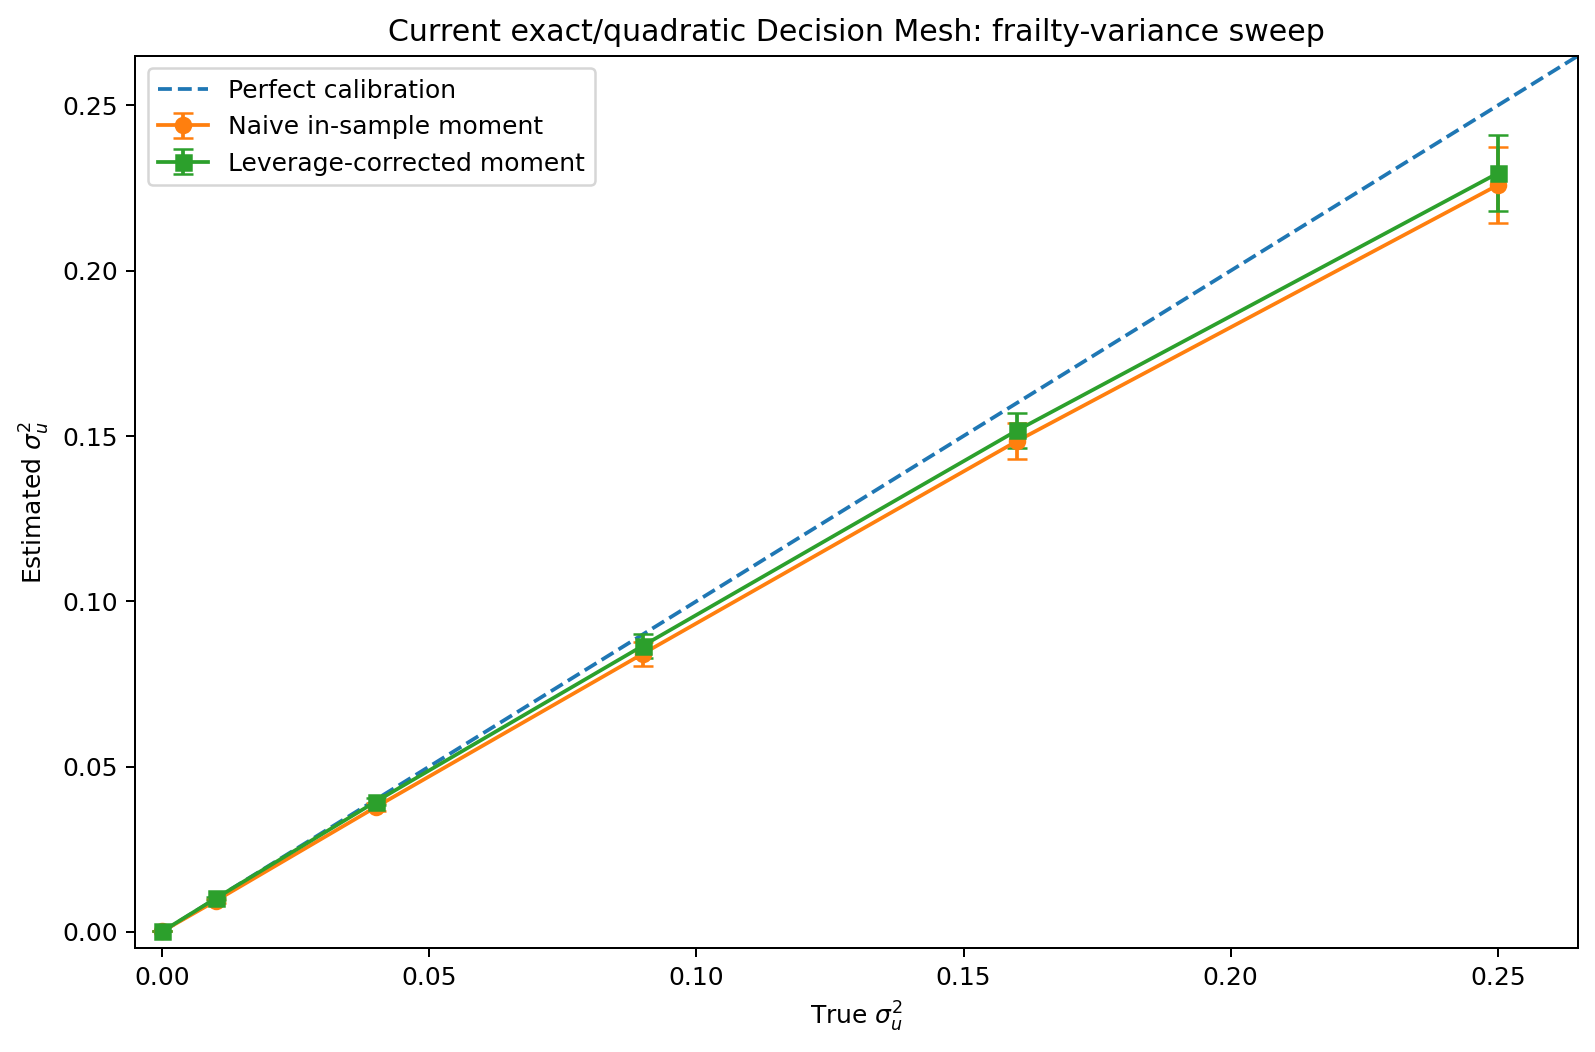
\includegraphics[width=\linewidth]{current_frailty_sweep.png}
\end{minipage}
\caption{Current exact/quadratic benchmark reruns. Left: among completed fits, held-out
surface RMSE continues to fall as $q$ increases, but $q=0.50$ has one deterministic
catastrophic run; $q=0.25$ is the strongest setting completing all five seeds. Right: the
analytic leverage correction improves variance calibration at every positive frailty level,
but residual downward bias grows to $8.2\%$ at $\sigma_u^2=0.25$.}
\label{fig:current-reruns}
\end{figure}


\begin{figure}[h]
\centering
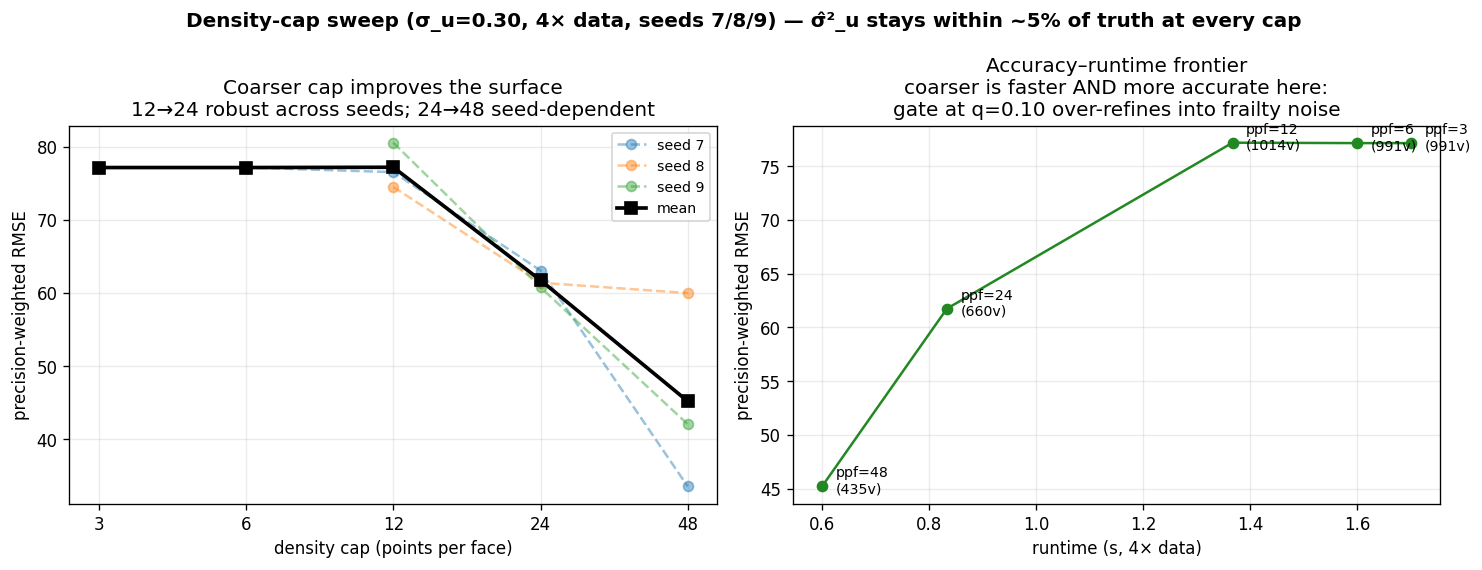
\includegraphics[width=\textwidth]{fig8_capsweep.png}
\caption{Density-cap sweep on the uniform surface (seeds 7/8/9). Tightening the cap from 12 to 24 pts/face improves precision-weighted surface RMSE on every seed while running $\sim$40\% faster: at $q=0.10$ the gate over-admits vertices that fit frailty-correlated noise, and the cap acts as variance control. $\hat\sigma_u^2$ is insensitive to the cap ($\pm5\%$ of truth throughout) and the no-frailty floor holds. Note the cap binds only at round granularity, so a large admission round can overshoot it (visible in the 48-pts/face spread). This ordering \emph{reverses} on multi-scale truth (Section~\ref{sec:chirp}).}
\label{fig:capsweep}
\end{figure}


\begin{figure}[h]
\centering
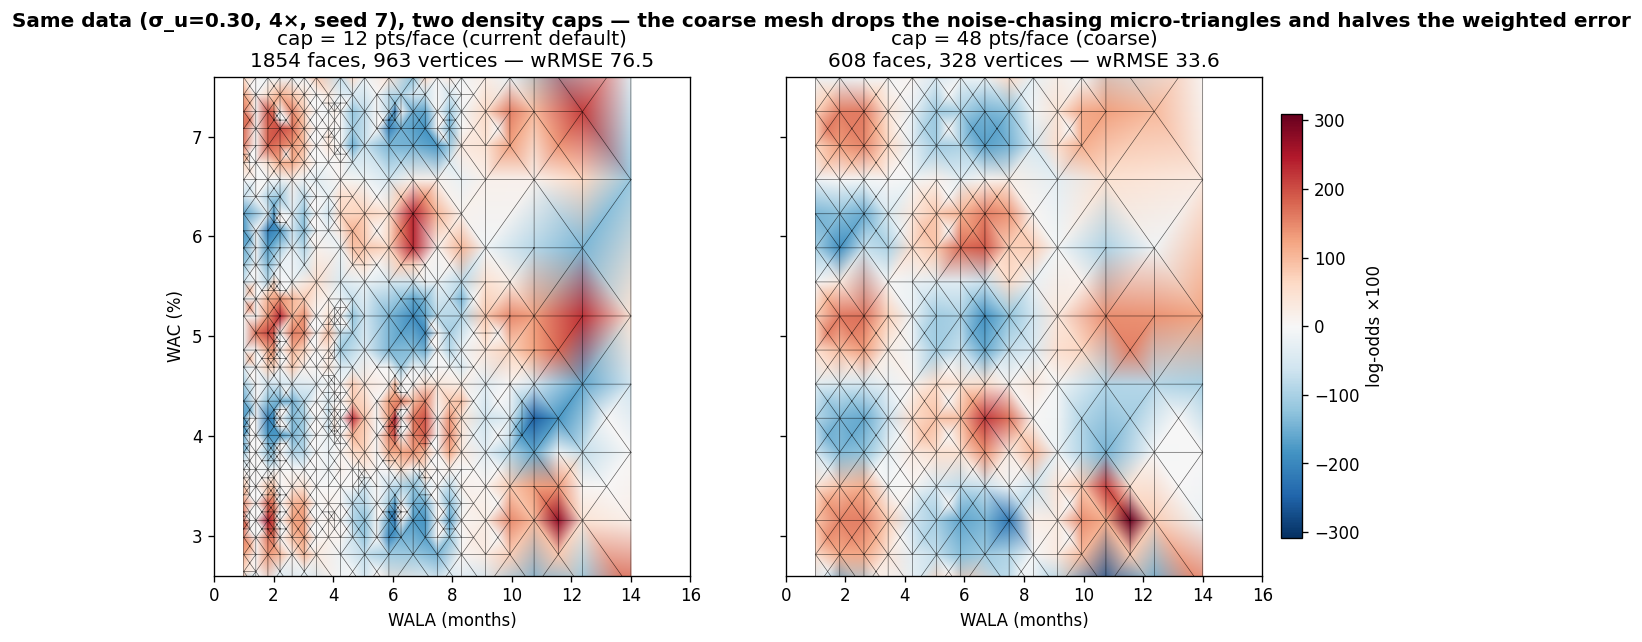
\includegraphics[width=\textwidth]{fig9_mesh_compare.png}
\caption{The cap's mechanism, visually: identical data under the 12- and 48-pts/face caps. The fine mesh carries clusters of noise-chasing micro-triangles in the dense band; the coarse mesh tessellates at the target's natural scale and halves the weighted error (most favorable seed shown; see Figure~\ref{fig:capsweep} for the seed spread).}
\label{fig:meshcompare}
\end{figure}



Unless labeled otherwise, the current reruns use the cohort-geometry generator, the exact
coupled solver, the quadratic inherited-child prior, and seeds 7--11. The table separates
current evidence from results inherited from older executables.

\begin{center}
\small
\begin{tabularx}{\textwidth}{@{}p{0.22\textwidth}X p{0.19\textwidth}p{0.16\textwidth}@{}}
\toprule
Experiment & Result & Reference value & Provenance\\
\midrule
Gaussian cosine, uniform sampling & fit error $0.121$, test MSE $1.13$ & noise floor $1.0$ & legacy Gaussian solver; rerun pending\\
Gaussian cosine, cohort geometry & fit error $0.047$, test MSE $1.034$ & noise floor $1.0$ & legacy Gaussian solver; rerun pending\\
Prepayment correction (binomial) & $94\%$ of systematic error removed & coordinate ceiling $\approx92\%$ & legacy adaptive pipeline; rerun pending\\
Frame attachment, cohort truth & Lagrangian rank-1 share $0.997$; $\hat\lambda=0.0196$ & $\lambda=0.02$ & legacy fitted nodal panel\\
Frame attachment, location truth & Eulerian rank-1 share $0.989$; $\hat\lambda=0.0250$ & $\lambda=0.02$ & legacy fitted nodal panel\\
Overdispersion at $\sigma_u=0.30$ & mean $\hat\sigma_u^2=0.08856$, seed sd $0.00390$ & $0.0900$ & current, five seeds\\
Known shift omitted & included $0.09106$, omitted $0.20512$; $93.1\%$ of $\beta^2$ recovered & $0.0900$, $0.2125$ & current matched audit\\
Frailty sweep & corrected calibration slope $0.9306$; bias $-8.2\%$ at truth $0.25$ & slope $1$ & current, 30 fits\\
Excess-moment comparison & bias $-0.011$, RMSE $0.038$ (best of five) & truth by construction & legacy; rerun pending\\
Double-dip correction & trace $-0.00005$, bootstrap $+0.00016$ & naive $-0.018$; target $0$ & legacy pool layer; rerun pending\\
Oracle pairwise moment (no fit) & bias $\le1\%$ across tested configurations & $\sigma_u^2=0.09$ & mechanism-level control\\
Leverage bracket & in-sample $0.083$, holdout $0.126$ & $0.090$ & legacy specialized holdout moment\\
$q$-sweep & $q=0.25$ best stable (5/5); $q=0.50$ lower conditional RMSE but 1/5 catastrophic & stable low miss & current, five seeds\\
\bottomrule
\end{tabularx}
\end{center}
\normalsize

The negative results now fall into two categories. Structural findings that remain current are:
empirical-logit responses cap recovery at $59\%$ (Section~\ref{sec:empiricallogit}); an
uncorrected theoretical $N(0,1)$ null can admit essentially everything; unconstrained central
matching can absorb a signal-dominated candidate family; one Gaussian variance shared across
\emph{sparse split-tree surpluses} can freeze refinement; and Eulerian gradient-based velocity
estimation is unidentified on one-dimensional cohort cross-sections. These statements do not imply
that pooled shrinkage is always harmful: one pooled parent variance is preferred for the later
orthogonalized geometric-cover basis.

Several other negative results are now historical postmortems rather than current limitations.
Partial exact-profile retrofits failed because they were grafted onto the stale hybrid solver; the
completed exact coupled solver resolves that numerical objection. The old mesh could not reach the
WALA boundary without an external ramp, whereas the exact solver reaches a WALA 0--2 fitted logit of
$-6.96$. The locally balanced linear-child audit exposed two topology-collapse seeds, but quadratic
inheritance rebuilds both at ordinary topology sizes. Likewise, broad split-genealogy branch pooling
remains rejected, while final-geometry patch sharing is modestly positive and crossed function-level
covers are strongly positive under frozen-topology evaluation.

\subsection{Balance-weighted outcomes and continuous WACLS exposure}
\label{sec:wacls-sims}

We repeated the main simulation battery with heterogeneous current loan sizes
and balance-weighted prepayments.  Individual balances were lognormal with
coefficient of variation one; the same underlying pools and loan-level
prepayment draws were evaluated once using literal loan counts and once using
the continuous pseudo-counts in \eqref{eq:wacls-counts}.  At this dispersion,
$n_{\mathrm{eff}}$ is roughly one half of the literal loan count, so the
experiment is also a substantial information-reduction stress test.

An isolated calibration with 250 loans and $p=0.20$ shows the reason for the
construction.  The Pearson-residual variance under the ordinary-average-size
proxy rises from $1.06$ at loan-size CV $0.25$ to $1.24$, $2.00$, and $3.20$
at CV $0.5$, $1.0$, and $1.5$.  The WACLS pseudo-count gives respectively
$1.00$, $1.00$, $1.02$, and $1.03$.  The variance correction is therefore
first-order exact, with only the expected finite-pool and Monte Carlo error.

Across 90 matched scenario--seed runs, using continuous rather than rounded
WACLS pseudo-counts changed surface RMSE by $-0.018$ on average (median
$-0.002$), improved RMSE in 53 of 90 runs, and changed the corrected persistent
variance by $-0.003$ on average.  Continuous exposure admitted about seven more
vertices on average, but produced no systematic gate inflation.  In particular,
the complete-null variance floor remained zero and the complete-null surface
RMSE was $0.015$ under both rounded and continuous forms.

The principal scenario results are:
\begin{center}
\begin{tabular}{@{}lrrrr@{}}
\toprule
Scenario & Count RMSE & WACLS RMSE & Count $\hat\sigma_a^2$ & WACLS $\hat\sigma_a^2$\\
\midrule
Uniform surface & 0.434 & 0.370 & 0.073 & 0.074\\
Chirp surface & 0.518 & 0.512 & 0.242 & 0.235\\
No frailty & 0.425 & 0.349 & 0.012 & 0.000\\
Complete null & 0.010 & 0.015 & 0.000 & 0.000\\
\bottomrule
\end{tabular}
\end{center}
The literal-count and WACLS fits become nearly indistinguishable as data
increase.  On the chirp, the WACLS persistent-variance estimate falls from
$0.258$ at $1\times$ to $0.130$ at $4\times$ and $0.100$ at $16\times$, against
truth $0.09$: unresolved fine-scale spatial structure is initially attributed
to the pool component and is reclaimed by the surface with resolution, exactly
as in the count experiments.  The persistent/white decomposition also retains
its ordering under continuous WACLS exposure, and the FDR-target sweep shows no
systematic increase in admissions or empirical FDP.

The learned axis metric remains effective: on the chirp it lowers WACLS surface
RMSE from $0.512$ to $0.240$ and the corrected persistent variance from $0.235$
to $0.113$.  Density caps of 12, 24, and 48 points per face were nonbinding at
the $1\times$ WACLS workload; the gate and information floor stopped first.
The conclusion is operational: use literal counts for count outcomes and
continuous WACLS pseudo-counts for balance outcomes when current-balance WACLS
is available.  Rounding the pseudo-counts is unnecessary and is retained only
for backward comparisons.

\subsection{Multi-scale chirp stress test}\label{sec:chirp}

To test behavior when the target's length scale varies across the state space,
we replace the uniform cosine with a chirp,
$f(x,y)=A\cos\!\big(0.625\,(y+4)^2\big)\cos(2x)$, whose instantaneous frequency
rises linearly from $0$ to $10$ rad/unit along the (fully populated) WAC axis;
total oscillation count matches the uniform surface. Four findings
(Figure~\ref{fig:chirp}).

First, the mesh adapts to local scale: median triangle extent per WAC band
tracks the local wavelength across the support. Second, at fixed data ($4\times$)
the error concentrates at the fine scale: precision-weighted RMSE by frequency
band is $61/75/90$ (slow/mid/fast). Third, and most consequential for the
pool layer: under-resolved fine scale is \emph{attributed to}
$\hat\sigma_u^2$, which rises to $0.12$--$0.16$ against a generative
$\sigma_u^2=0.09$. This is the intended accounting, not a failure: the
estimator's contract is to measure signal left over, and fast-band miss is
pool-persistent (pools ride cohort trajectories at essentially fixed WAC), so
at the current resolution it \emph{is} pool-indexed unexplained signal. The
energy estimator tracks its oracle throughout; only the attribution between
shared-spatial and pool-idiosyncratic moves. Consistent with this reading, the
density-cap ordering flips relative to the uniform surface (finer mesh wins,
$0.122$ at 12 pts/face vs.\ $0.154$ at 24): on multi-scale truth the coarse
cap converts resolvable signal into reported $\hat\sigma_u^2$ rather than
discarding noise, and upward drift of $\hat\sigma_u^2$ under
refinement-starving is the flag that refinement (or a finer cap) still has
signal to claim.
Fourth, consistency restores the estimate: at $16\times$ data with a loose cap
the gate refines to $8{,}407$ vertices, resolves the fast band, and the
leverage-corrected $\hat\sigma_u^2$ returns to $0.0933$ ($+3.7\%$).

\begin{figure}[h]
\centering
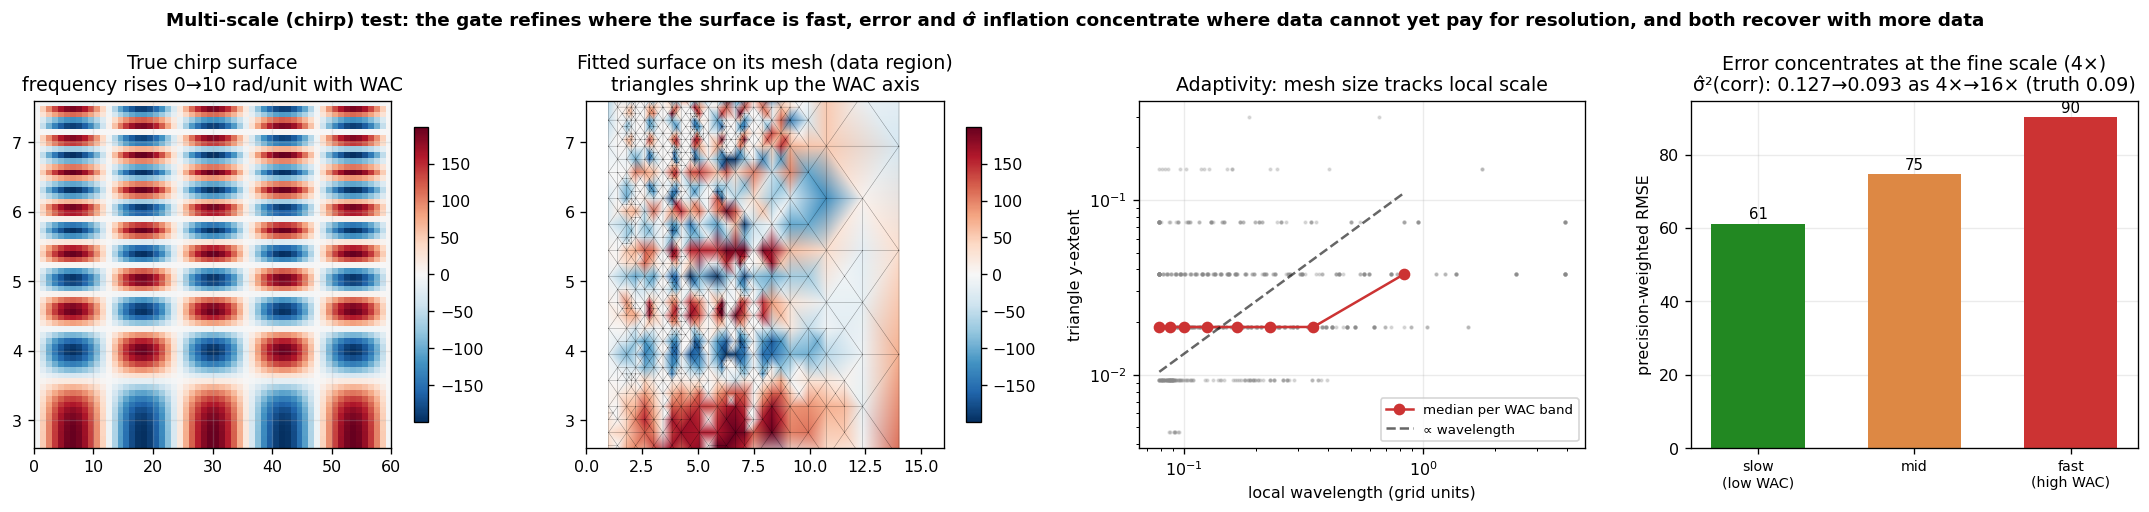
\includegraphics[width=\textwidth]{fig12_chirp.png}
\caption{Chirp stress test ($\sigma_u=0.30$, $4\times$ data unless noted).
Left to right: true surface; fit on its adaptive mesh (triangles shrink up the
WAC axis); triangle extent vs.\ local wavelength (medians track the
$\propto\lambda$ reference); weighted RMSE by frequency band, with the
$\hat\sigma^2_u$ recovery $0.127\to0.093$ from $4\times$ to $16\times$.}
\label{fig:chirp}
\end{figure}


\begin{figure}[ht]
\centering
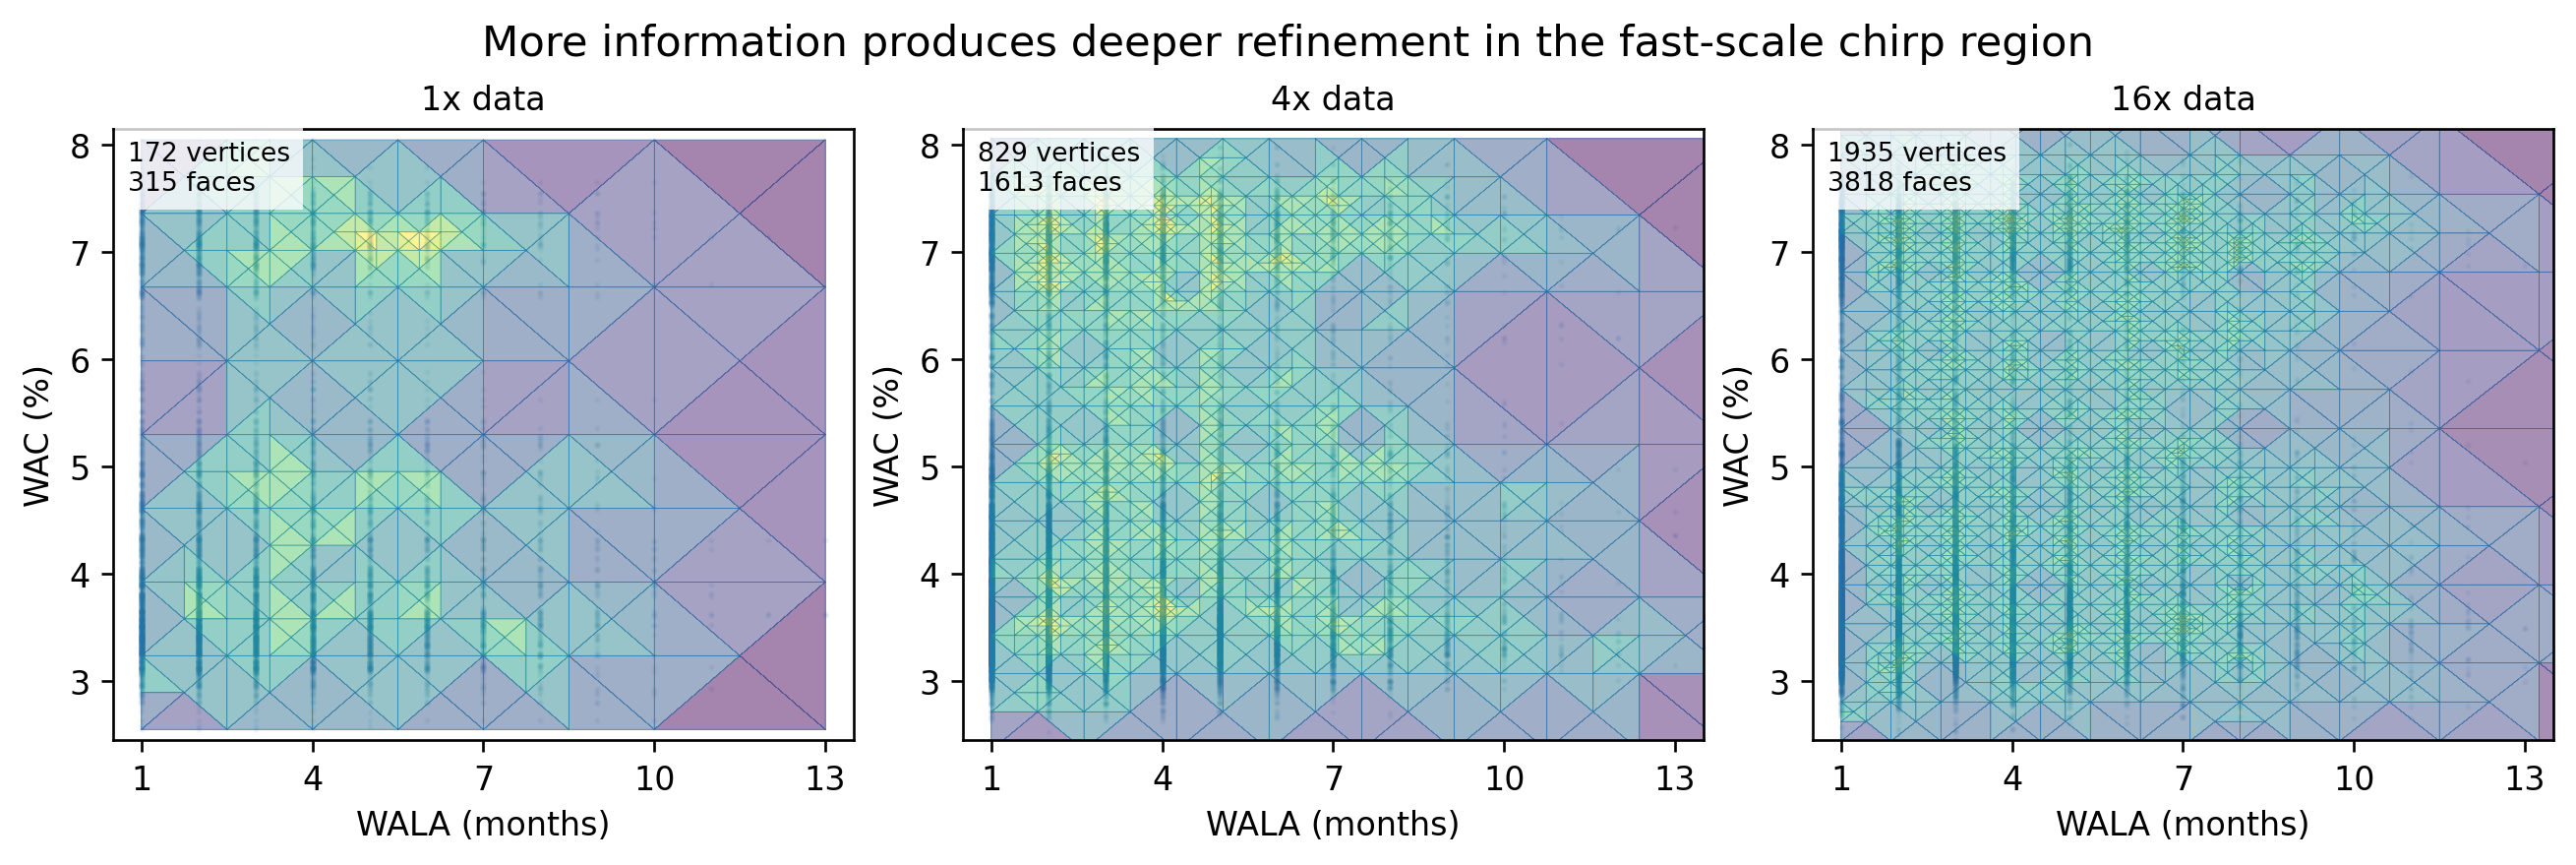
\includegraphics[width=\textwidth]{fig22_chirp_mesh_scaling.png}
\caption{Final chirp meshes at $1\times$, $4\times$, and $16\times$ information under continuous WACLS exposure. The physical WALA--WAC window and target are fixed. Increasing information permits progressively deeper refinement in the high-frequency region, providing a geometric view of the simultaneous fall in surface error and return of the persistent-variance estimate toward its generative value.}
\label{fig:chirp-mesh-scale}
\end{figure}

At $V=8{,}407$ the correction's dense LU factorization became the bottleneck
(183s, $O(V^3)$); since $A_\Lambda$ has $\sim$7 nonzeros per row (P1 elements
plus the 3-point ridge stencil), we replaced it with CSR storage and
Jacobi-preconditioned conjugate gradients for the Hutchinson probe solves,
reproducing the dense results to every reported digit at $O(\mathrm{nnz})$ per
iteration: the correction drops to 1.6s at that size and the pipeline remains
dependency-free.

\subsection{Attribution semantics: what $\hat\sigma_u^2$ means under underfit}
\label{sec:attribution-semantics}

How much of the chirp's $\hat\sigma_u^2$ inflation is recoverable as
\emph{shared} structure? A lag-matched contrast makes the attribution
operational: within-pool pairs sit at month-lags along cohort trajectories, so
we compare them to cross-pool pairs at the same displacement within a WAC band
--- shared spatial miss enters both equally at matched lag, frailty only the
within-pool side, and the difference estimates the idiosyncratic component.
The estimator is exact under the oracle (truth-residual cross moment $=0.0000$
on the uniform surface) and clean in the resolved regime: uniform $4\times$
gives shared $-0.001$ and idiosyncratic $0.079$, reproducing the naive
$\hat\sigma_u^2$. On the chirp the contrast recovers only part of the excess,
and sharpening the matching resolution saturates (shared $0.014/0.021/0.023$
and idiosyncratic $0.140/0.134/0.131$ at $24/48/96$ WAC bands, within-pool
moment $0.154$): the unresolved miss amplitude itself varies below band scale,
so its cross-pool average is recovered while its cross-pool \emph{variance}
remains pool-indexed. This is an identifiability boundary, not an estimator
defect: the shared/idiosyncratic split is defined only relative to a
resolution, and structure below the current resolving power is observationally
equivalent to frailty. The practical diagnostic follows: sweep the refinement
budget (or data) and read the profile of $\hat\sigma_u^2$; a declining
segment is resolvable signal being reclaimed by the surface ($0.154\to0.093$
from $4\times$ to $16\times$ here), and the plateau is the part entitled to
the name frailty.

\subsection{Learned axis metrics, and what the unit-square rescale actually is}
\label{sec:metric}

The rescale of $(\text{WALA},\text{WAC})$ to the unit square is not a numerical
convenience: newest-vertex bisection has no in-plane direction choice (the
refinement edge is dictated by the tree, and the finite similarity-class
structure is what guarantees shape regularity, conforming closure, and the
chord-routing invariant), so the coordinate map is the \emph{only} anisotropy
control, and mapping both axes to $[0,1]$ silently declares one full WALA range
equal to one full WAC range in difficulty at every depth. The algorithmic
version of ``incorporate the relative scales'' is therefore to learn the map:
after the stage-0 pilot fit we estimate density-weighted directional curvature
energies per axis band and equidistribute each axis by
$\Phi'\propto|f''|^{1/2}$ (knot density for $P_1$ error $h^2|f''|$), a
piecewise-linear monotone reparametrization (\texttt{DMESH\_METRIC=1}).

Two findings temper and sharpen the idea. First, on the chirp with a loose
refinement budget the learned metric is nearly immaterial for surface error
(weighted RMSE $70.2\to71.2$): the lfdr gate already performs the
equidistribution itself through refinement depth (Figure~\ref{fig:chirp},
third panel), and the fast band is data-limited, not parametrization-limited.
Second, in the \emph{budget-limited} regime (24 pts/face) the metric
reallocates scarce resolution and acts mainly through the frailty channel:
corrected $\hat\sigma_u^2$ falls from $0.162$ to $0.124$ (against truth
$0.09$) with $10\%$ fewer vertices, because thinner fast-band strips make the
residual miss vary within pools rather than ride them, cutting the
pool-persistent leakage into the pairwise moment. The uniform-surface results
are unchanged under the learned map, and the no-frailty floor rises mildly
($0.0003\to0.0010$; the pilot fit's noise curvature warps the map when there
is no signal), so the option defaults off. Genuinely local anisotropy
(directional ratios varying point to point) is out of reach of any separable
map and of isotropic NVB; the general tool is metric-field remeshing or
dimension-adaptive tensor bases, which we note as the larger lift. Single-seed
numbers throughout this subsection.


\subsection{Implementation cost}
\begin{figure}[h]
\centering
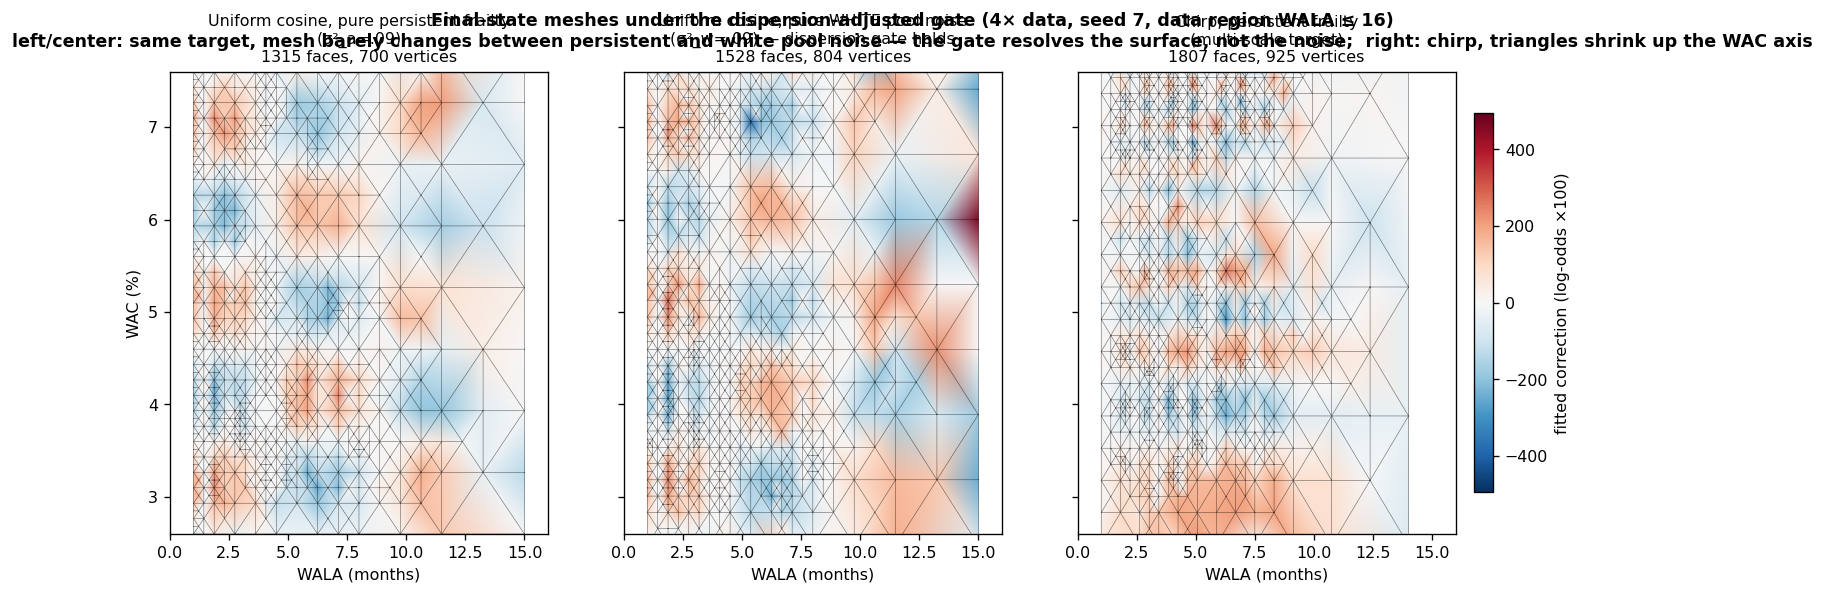
\includegraphics[width=0.75\textwidth]{fig7_optimization.png}
\caption{Implementation cost at the $8\times$ workload (46k pool-months), log scale: Python baseline through the C++ port, stage-0 cap, Hutchinson diag($S$), container refactor, and heap disable. The subsequent sparse-CG solve (Section~\ref{sec:chirp}) removes the remaining $O(V^3)$ term in the correction.}
\label{fig:speed}
\end{figure}

\paragraph{Frozen exact-solver release benchmark.}
To make the implementation timing reproducible, the July 29 release freezes a
single Ginnie design benchmark: 120{,}595 rows, an even--odd held-out split,
$q=0.10$, 24 points per face, exact likelihood fitting, the legacy-calibrated
stage-0 pilot, the B3 signed-root score in later stages, and gate extra variance
$0.35$.  In a clean native Release build on the release machine, the complete
run took 7.43 seconds with direct candidate BH and 6.51 seconds with the
adaptive Lindsey gate; the program-internal totals were 7.1 and 6.2 seconds.
These totals include final hierarchical retirement and refitting, leverage and
PM diagnostics, and CSV export.  The adaptation timestamps through stage 2
were 4.9 seconds for BH and 4.5 seconds for Lindsey.  This distinction matters:
earlier development shorthand that described a ``4/7-second build'' mixed an
adaptation timestamp with full executable wall time.  The release therefore
ships the benchmark data, exact environment, reference output hashes, and a
verification script.  The accepted speed changes are an exact stage-convergence
stop, Release-mode $-O3$ with optional native tuning and LTO, and one-time
materialization of sparse likelihood rows within each height solve.  Candidate
column caches and descendant-only traversals that changed the adaptive path are
excluded.

\section{Real-data check: Ginnie Mae pools and the EB ablation}\label{sec:realdata}

We ran the full C++ pipeline on the Ginnie Mae single-family pool portfolio
disclosure for April 2026 (\texttt{monthlySFPS\_202604}): 120{,}595 SF pools
covering 47M currently disclosed loans after basic filters, including the
multi-issuer mega-pools (up to $\sim$150k loans). A single monthly snapshot
contains no monthly prepayment outcome and therefore does not identify SMM.
The development dataset instead constructed
\[
 \widetilde n_0=\mathrm{round}(\text{OrigAggregate}/\text{AOLS}),\qquad
 k_{\mathrm{proxy}}=\widetilde n_0-n_{\text{now}}.
\]
This is a \emph{loan-count attrition proxy}, not an exact original loan count
and not an exact cumulative-termination response. Original Aggregate is fixed
at issuance, whereas AOLS is the simple average original size of loans in the
currently disclosed pool composition. If terminated and surviving loans have
different original sizes, their ratio need not recover the number of loans at
issuance. Here $n_{\text{now}}$ is the disclosed current number of loans; Pool
UPB divided by an average loan size is also not a current-loan count because it
falls under scheduled amortization even without termination. A
balance-weighted monthly hazard would require a panel or loan-level balances
and the continuous exposure in \eqref{eq:wacls-counts}, neither of which is
available in this single pool-level snapshot.

Subject to that measurement qualification, the gated mesh fits the constructed
attrition-proxy surface over $(\text{WALA},\text{WAC})$ from a constant-offset
start. The earlier 3{,}103-vertex fit and its dispersion diagnostics remain
useful as an estimator stress test, but their probabilities must not be called
SMM. The dispersion calibration of Section~\ref{sec:poolstate} reduced the
residual energy read from $0.25$ to $0.16$, the uncalibrated gate having
over-admitted on these constructed counts exactly as in the pure-white
simulation.
With one observation per pool, the pairwise moment has no within-pool pairs, so the
\emph{persistent-versus-temporary} decomposition of pool heterogeneity is not identified from this
snapshot alone. This does not prevent one-shot empirical-Bayes attribution. Conditional on the fitted
cross-sectional pool law, the credibility update in Section~\ref{sec:posthoc} gives a posterior mean
$\hat u_P$ for every pool. Throughout the real-data figures below, ``pool effect'' means this posterior
current deviation; no claim of permanence is attached to the label.


\subsection{Outcome-construction caveat and WALA-zero sensitivity}\label{sec:wala0-audit}

The WALA-zero slice exposed the count-reconstruction problem directly. In the
WAC 5--6\% band, the constructed proxy implied roughly 36\% attrition at
WALA~0; one large observation generated about 74\% of the implied attritions
in that slice. Such a value is not credible as SMM and is not persuasive as an
exact cumulative-termination count for newly issued collateral. The main
permutation-gate comparison was therefore repeated after removing all 460
WALA-zero pools, leaving 120{,}135 observations. We first rescored the existing
fits without WALA~0 and then refit both estimators from scratch on ten matched,
locally balanced train--held-out splits.

\begin{table}[H]
\centering
\small
\caption{Real Ginnie proxy fit after removing WALA~0 and refitting. Values are
means across ten matched splits. Lower held-out deviance and $X^2$/information
are better.}
\label{tab:no-wala0-real}
\resizebox{\textwidth}{!}{%
\begin{tabular}{lrrrrr}
\toprule
Gate & Deviance/pool & $X^2$/info & Admissions & Faces & Max depth\\
\midrule
Shipped Lindsey, $q=.10$ & 6.4968 & 0.15237 & 118.0 & 729.8 & 8.7\\
Pooled permutation BH, $K_{\mathrm{eff}}\ge4$, $q=.15$ & 6.8108 & 0.15857 & 136.1 & 885.9 & 6.1\\
\bottomrule
\end{tabular}%
}
\end{table}

The permutation fit remained worse in all ten splits. Its mean paired deviance
increase was $0.3140$ per pool, with a split-bootstrap interval
$[0.2328,0.3970]$. Before the exclusion the gap was $0.5615$, so WALA~0
explained about 44\% of the apparent loss, but not all of it. The shipped gate's
mean admitted count fell from 187.7 to 118.0 after removal, while the
permutation count moved only from 143.1 to 136.1. Thus the shipped estimator
had spent substantial capacity fitting the suspect boundary feature. The
remaining loss is concentrated first at WALA 1--5 and then in smaller bands at
higher ages; this is a power problem for localized structure, not evidence that
the WALA-zero spike was genuine mortgage behavior.

\begin{figure}[H]
\centering
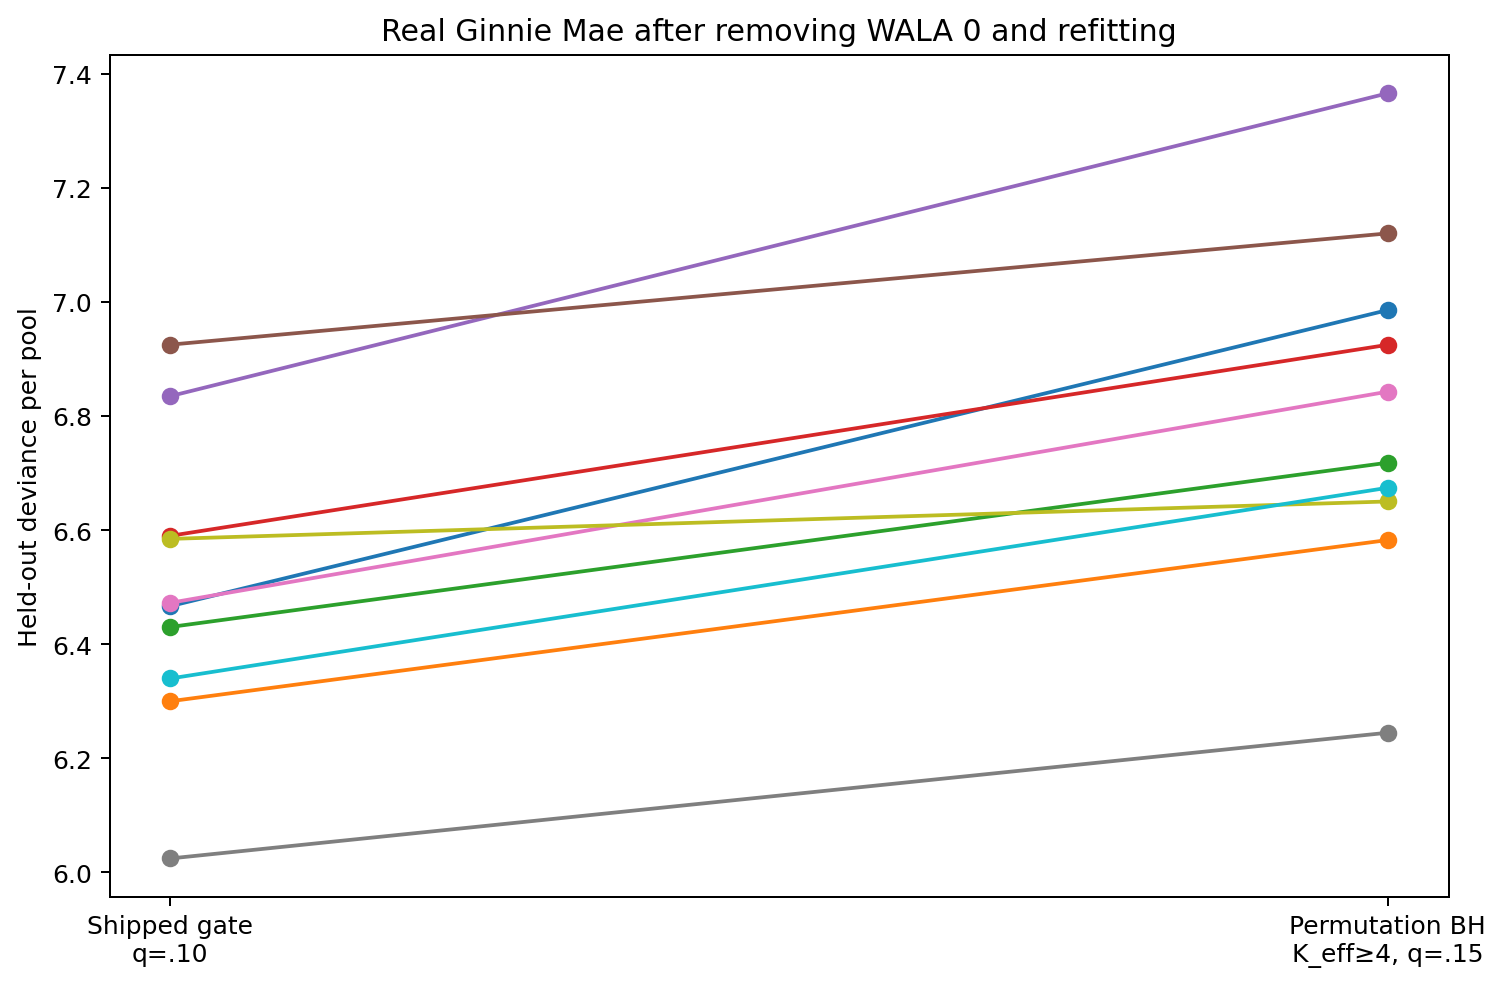
\includegraphics[width=0.78\linewidth]{no_wala0_paired_heldout_deviance.png}
\caption{Paired held-out deviance after removing WALA~0 and refitting. Each
line is one deterministic locally balanced split. The pooled-permutation gate
is worse in all ten splits, although the gap is materially smaller than in the
unfiltered comparison.}
\label{fig:no-wala0-paired}
\end{figure}

The real data gives the shrinkage layer a demanding test: the median GNMA~II
custom pool contains 13 loans at origination, so thousands of mesh vertices
are supported by a handful of tiny pools. An ablation isolates the effect:
fitting on even-indexed pools and scoring held-out odd-indexed pools, with
empirical-Bayes shrinkage on versus off (raw local WLS heights).

\begin{figure}[h]
\centering
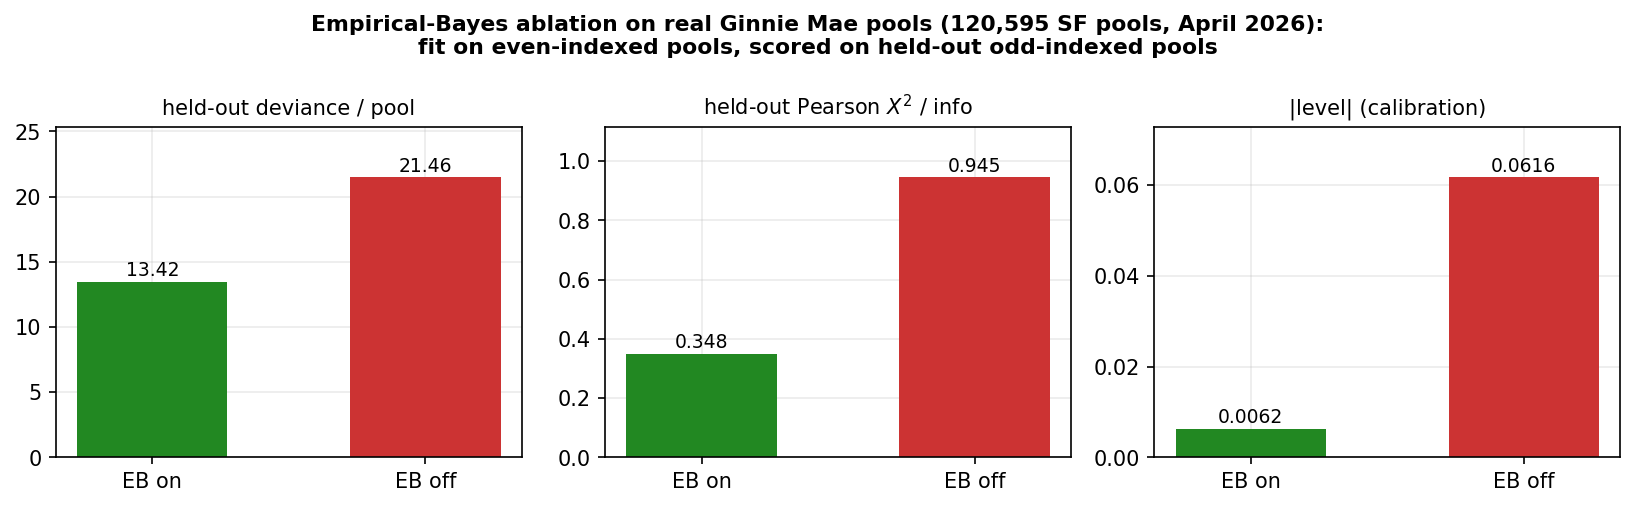
\includegraphics[width=\textwidth]{fig11_eb_ablation.png}
\caption{EB ablation on held-out real pools. Removing shrinkage raises
held-out deviance by 60\% (13.4 to 21.5 per pool), nearly triples Pearson
$X^2$ per unit information (0.35 to 0.95), and degrades the level calibration
tenfold ($-0.006$ to $-0.062$). Without shrinkage the candidate $z$-scores are
also wilder, so the gate over-admits (3{,}290 vs.\ 2{,}854 vertices),
compounding the overfit. The only quantity EB costs is fit time (2.5s vs.\
1.1s).}
\label{fig:ebablation}
\end{figure}

The ablation confirms on real data the small-cell noise mechanism that
motivated the hierarchical prior: unshrunk heights on thin support are
essentially noise, and the depth-indexed EB precision $1/\tau_d^2$ removes it
at the cost of a factor of two in fit time.

\subsection{Posterior pool effects and observed heterogeneity}\label{sec:ginnie-pool-effects}

The Lindsey-calibrated real-data run was continued through the credibility and variance-law
iterations, yielding a posterior pool effect for every one of the 120{,}595 observations. The C++
dump stores these values in centi-log-odds; the figures convert them to ordinary log-odds units.
Figure~\ref{fig:ginnie-pool-scatter} plots every pool at its original WALA and WAC coordinates. The
points themselves are not filtered; only the color scale is clipped at the first and ninety-ninth
percentiles so that the cross-sectional structure remains visible.

\begin{figure}[t]
\centering
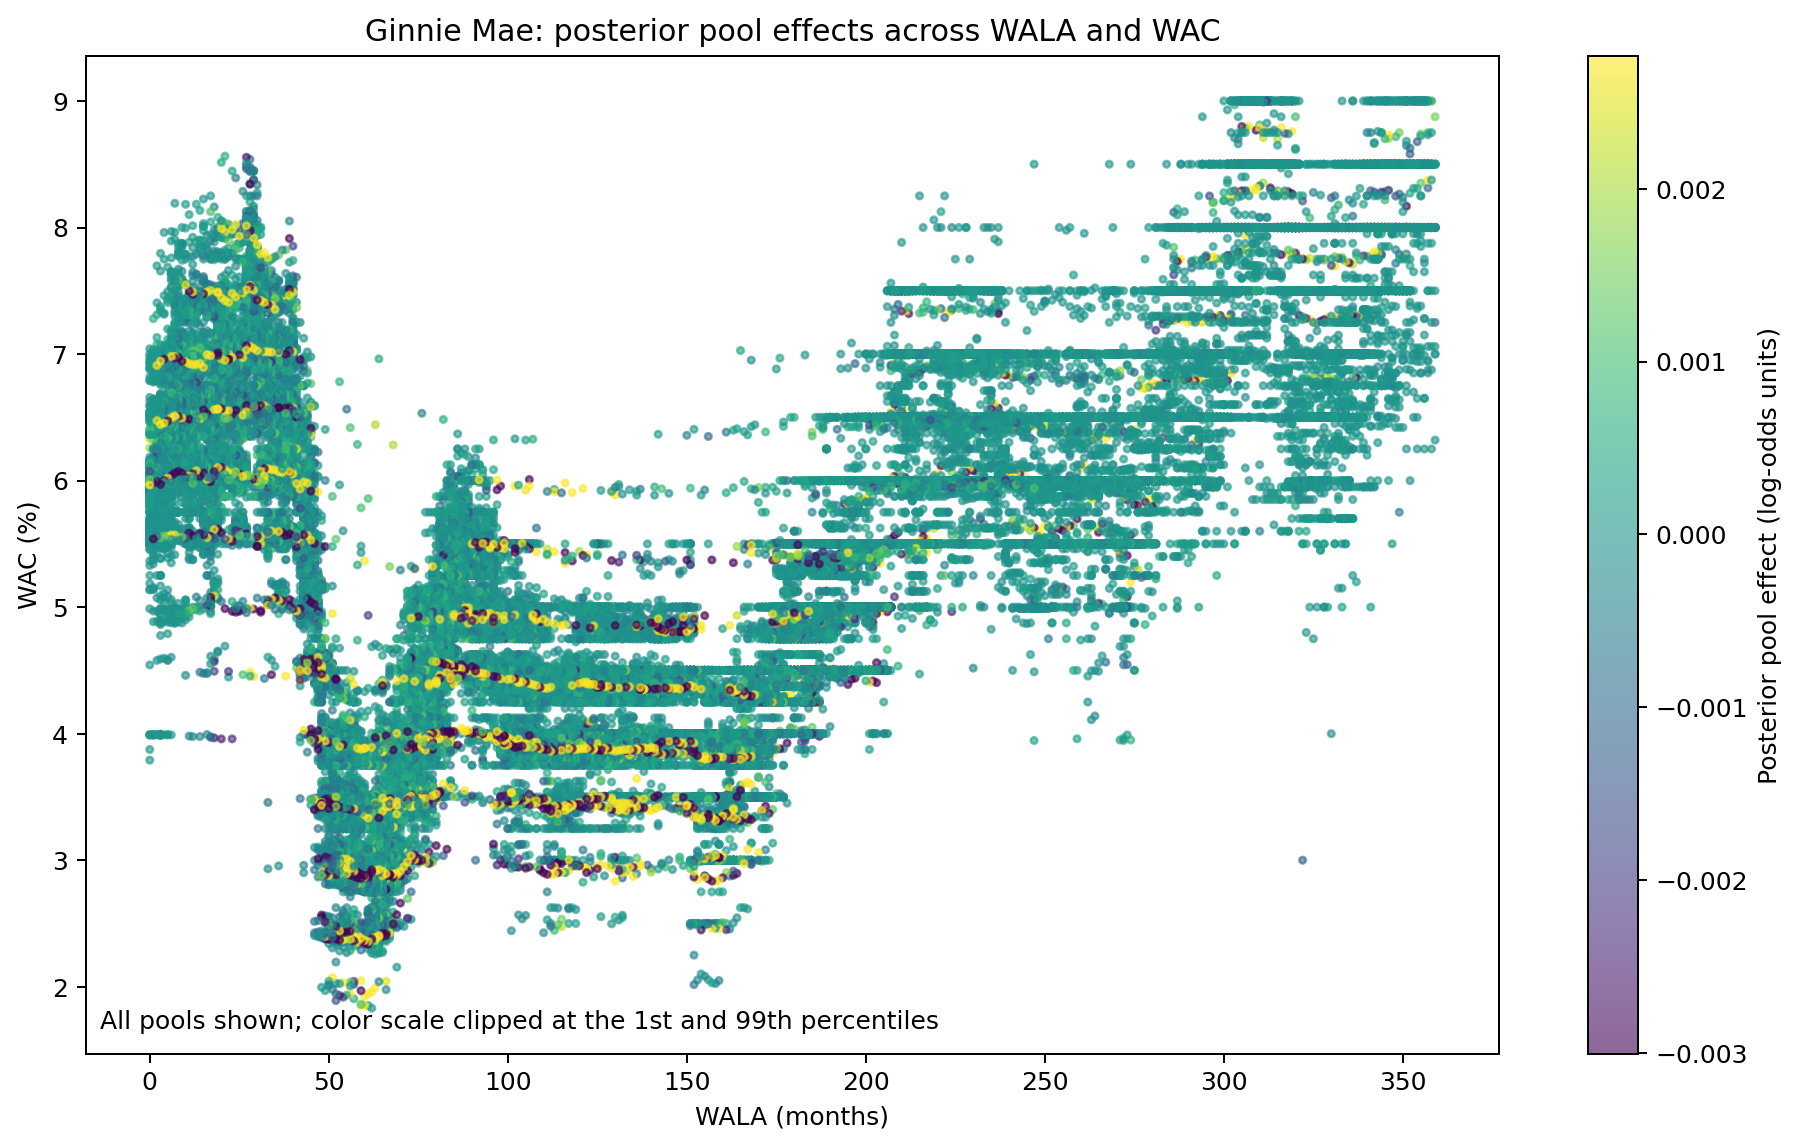
\includegraphics[width=0.94\linewidth]{ginnie_posterior_pool_effect_scatter.png}
\caption{Posterior pool effects across the full Ginnie Mae WALA--WAC support. Every one of the
120{,}595 pools is plotted. The color scale is clipped at the first and ninety-ninth percentiles for
readability, but no pools are removed. The line and cohort structure shows that the remaining
heterogeneity is localized rather than exchangeable white noise after conditioning only on WALA and
WAC. Effects are posterior current deviations and need not be permanent.}
\label{fig:ginnie-pool-scatter}
\end{figure}

The center of the posterior distribution is extremely concentrated: the median effect is
$1.9\times10^{-5}$ log-odds, and the first and ninety-ninth percentiles are approximately
$-0.0030$ and $+0.0028$. The distribution nevertheless has long diagnostic tails: the 0.1 and
99.9 percentiles are about $-0.0777$ and $+0.0813$, while the most extreme posterior means are
$-0.678$ and $+0.461$. These tails are why a single standard deviation is not a sufficient visual
summary of the heterogeneity.

\begin{figure}[t]
\centering
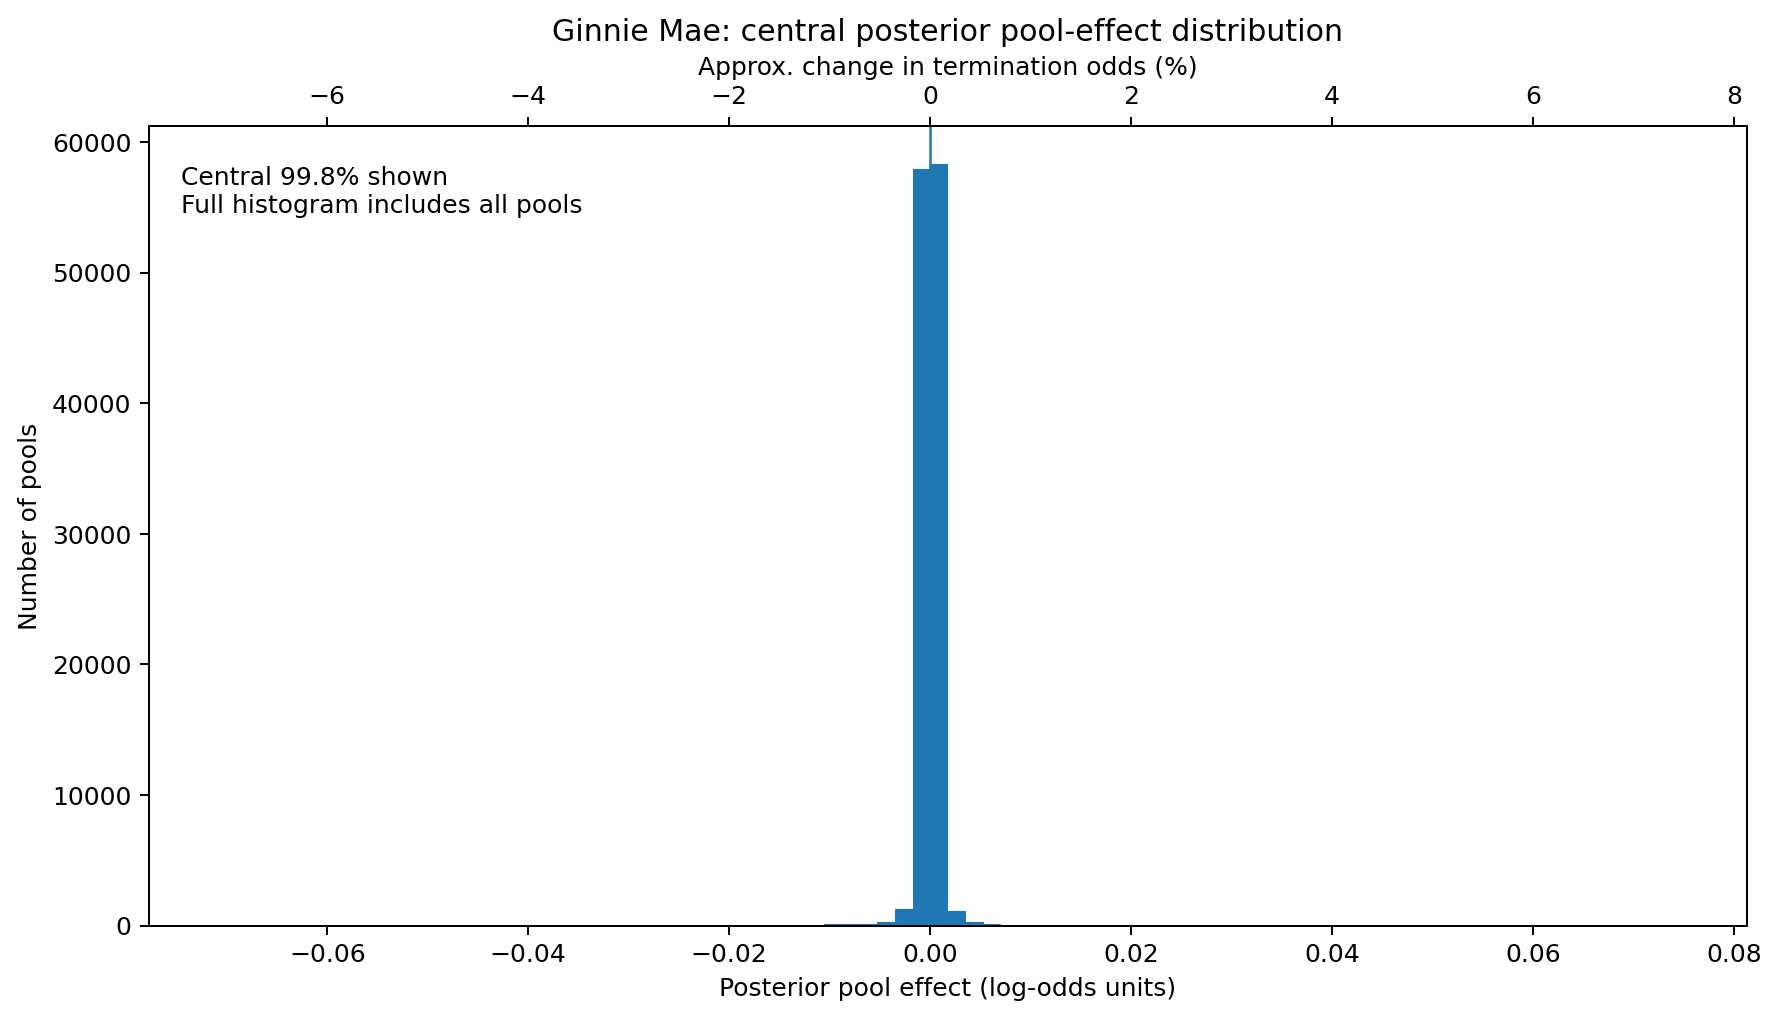
\includegraphics[width=0.84\linewidth]{ginnie_posterior_pool_effect_hist_central.png}
\caption{Central 99.8\% of the posterior pool-effect distribution. The lower axis is in log-odds
units; the upper axis shows the first-order approximation $100\hat u_P$ percent. For modest effects
this can be read as an approximate percentage change in the constructed attrition-proxy odds. The full-tail view is shown
in Figure~\ref{fig:ginnie-pool-all}.}
\label{fig:ginnie-pool-histograms}
\end{figure}

\begin{figure}[t]
\centering
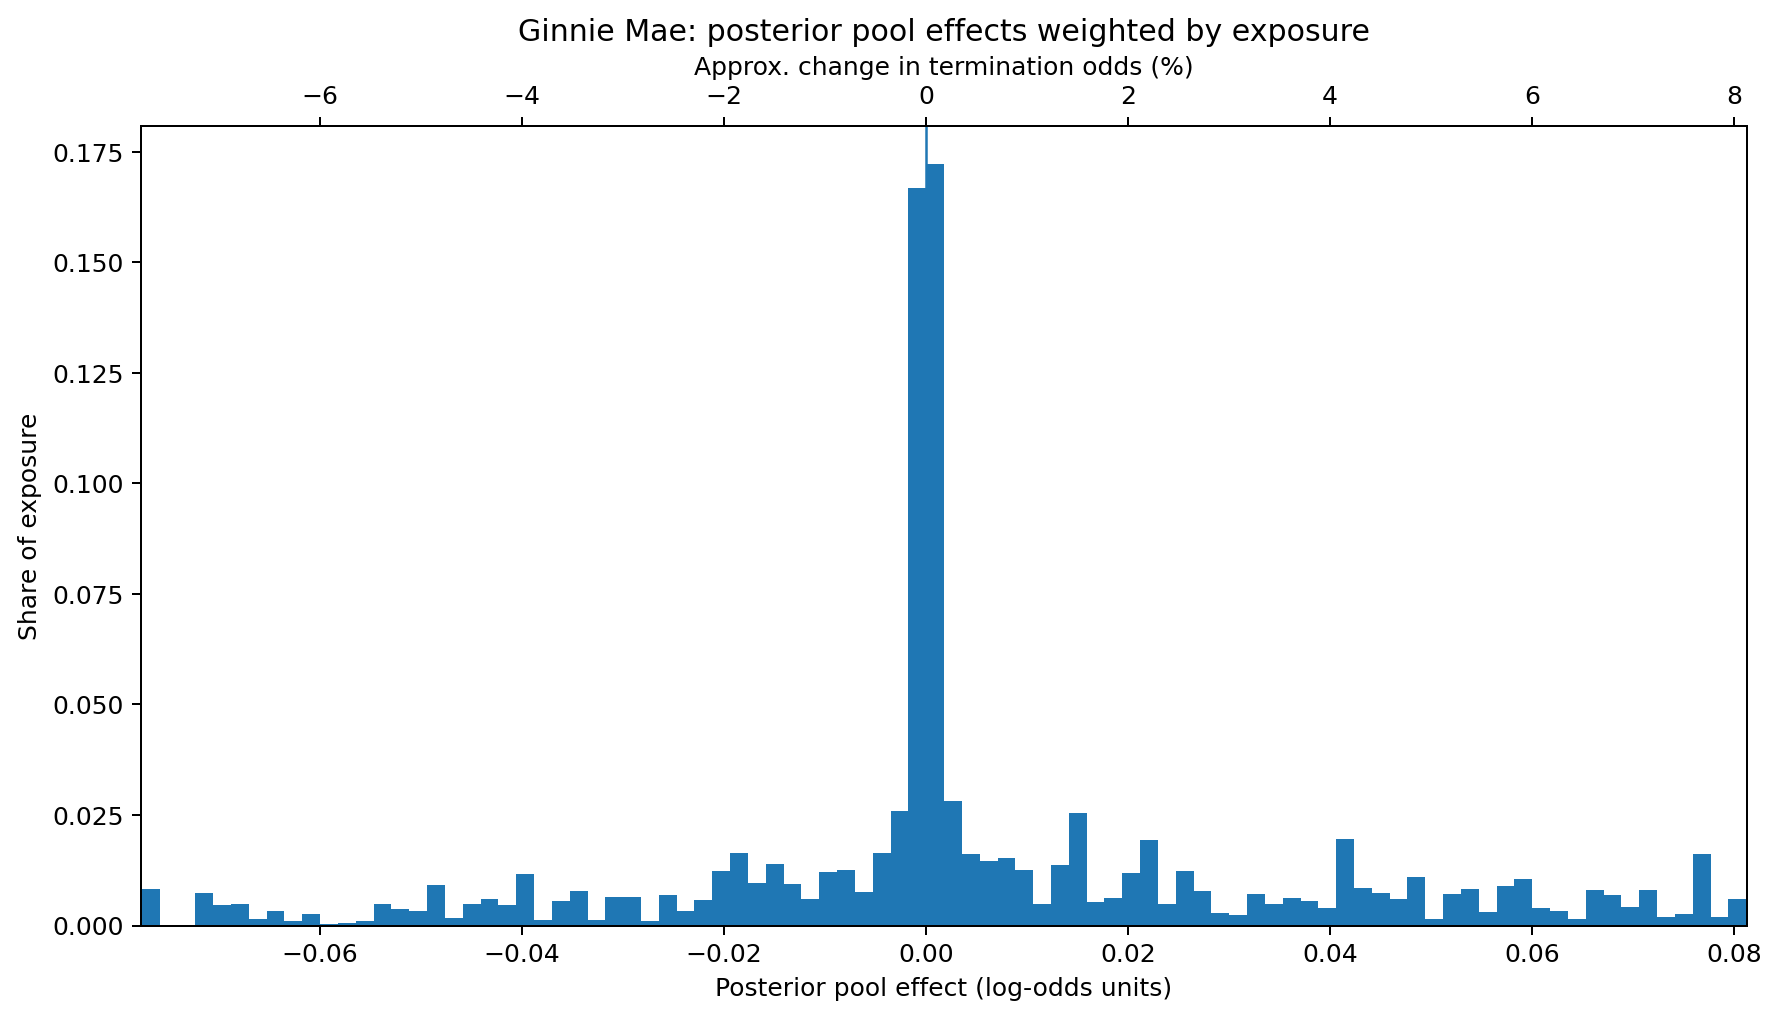
\includegraphics[width=0.84\linewidth]{ginnie_posterior_pool_effect_hist_weighted.png}
\caption{The same central posterior pool-effect range weighted by pool exposure. Large pools receive
proportionally more visual mass, so this panel emphasizes heterogeneity where more of the portfolio is
located rather than giving every pool equal weight.}
\label{fig:ginnie-pool-weighted}
\end{figure}

\begin{figure}[t]
\centering
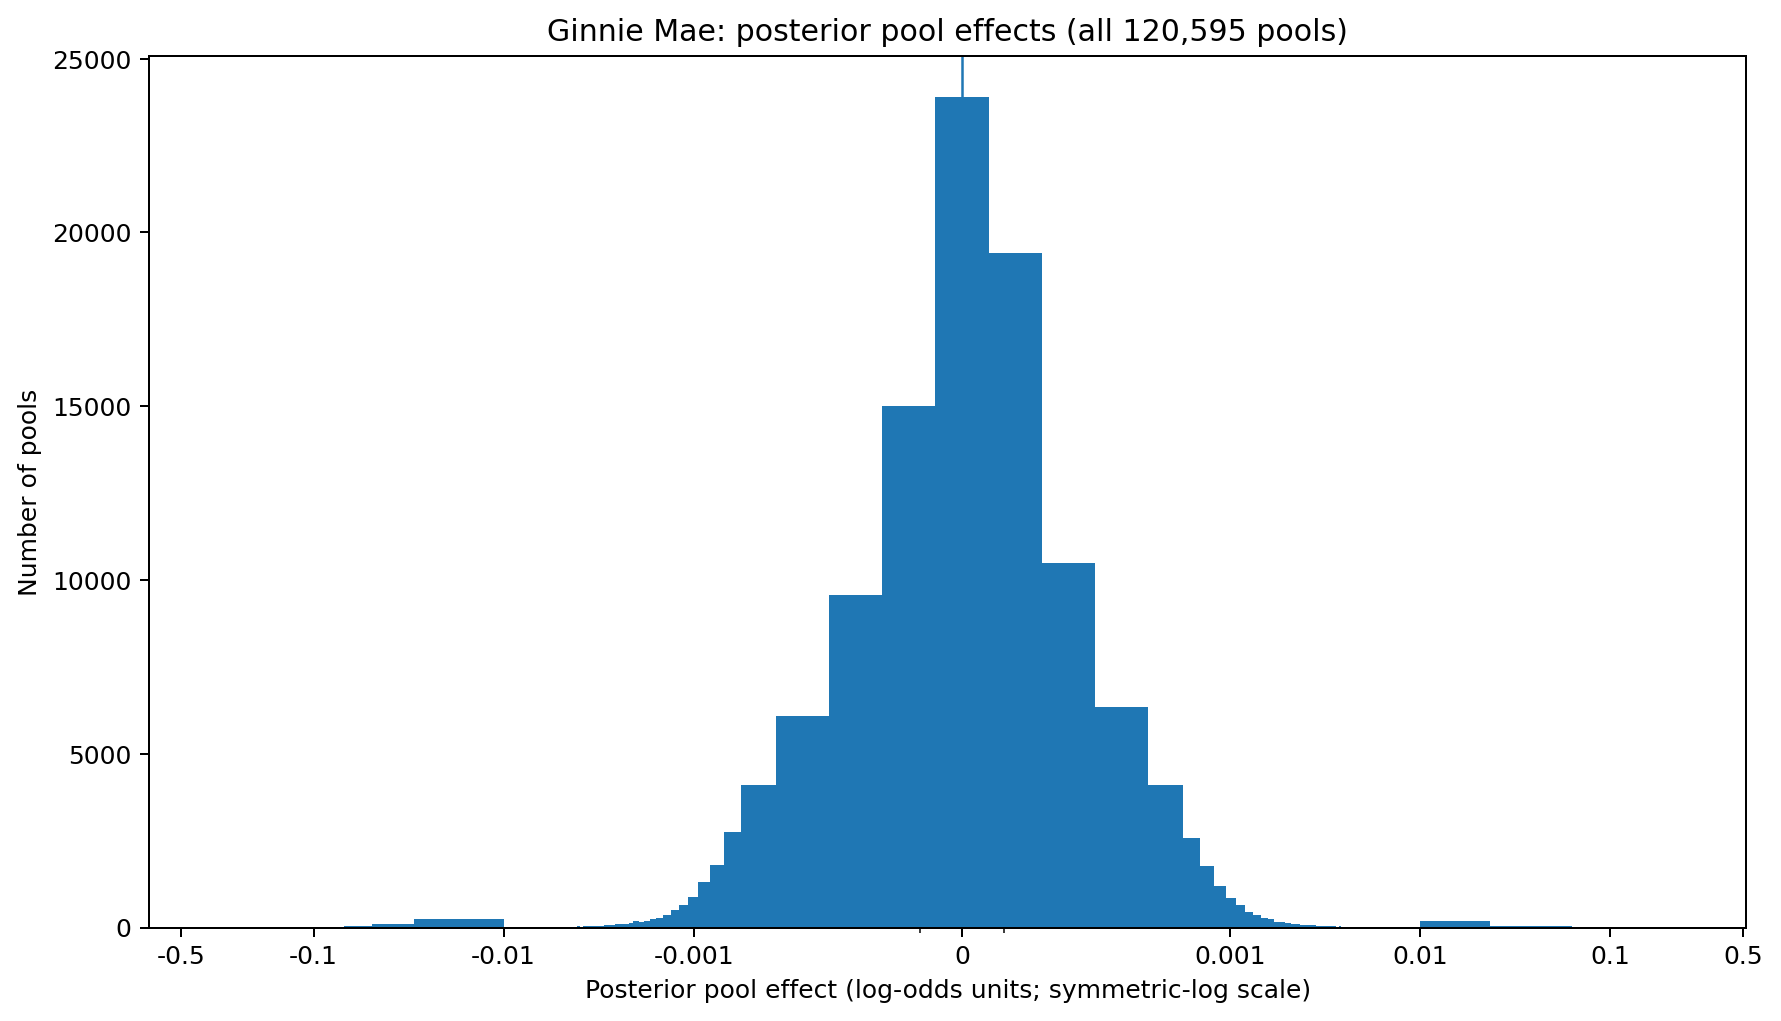
\includegraphics[width=0.82\linewidth]{ginnie_posterior_pool_effect_hist_all.png}
\caption{All 120{,}595 posterior pool effects. A symmetric-log horizontal scale preserves the sharply
concentrated center while retaining the extreme tails. Unlike the central presentation panels in
Figure~\ref{fig:ginnie-pool-histograms}, this histogram includes every posterior effect.}
\label{fig:ginnie-pool-all}
\end{figure}

These figures change the interpretation of the residual layer. The relevant output is not a single
``unexplained variance'' number. It is a distribution of posterior attributions: most pools remain
close to the shared WALA--WAC surface, while a small but consequential subset departs materially.
Those departures may reflect temporary shocks, omitted pool characteristics, or local surface miss.
A panel is required to separate those mechanisms, but not to estimate the current posterior effects
shown here.

\section{Updated controlled benchmark and deep-refinement diagnostics}\label{sec:updated2026}

This section records the July 2026 revisions to the simulation design and the subsequent
Ginnie Mae diagnostics.  These experiments sharpen two distinct questions that were
confounded in the earlier development runs: whether the mesh places resolution correctly
when the sampling support is benign, and whether hierarchical empirical-Bayes shrinkage
remains sufficiently strong after many successive refinements in real data.

\subsection{Uniform-support benchmark with increasing spatial frequency}

The default controlled simulation now removes the cohort-support artifact.  WAC is drawn
independently over its full range, every simulated pool is observed at WALA 1--60, and
there is no attrition.  The displayed horizontal coordinate is
\[
 x=\mathrm{WALA}/12\in[1/12,5].
\]
The target remains the two-scale exponential-cosine surface, but its normalized horizontal
coordinate $z\in[0,1]$ is warped according to
\[
 z_{\mathrm{warp}}=(0.2+0.8z)z.
\]
Thus the local horizontal frequency increases smoothly toward larger WALA while the data
remain essentially uniform over the rectangle.  This design is intended as a geometric
identification experiment rather than a realistic mortgage-vintage model.

In the representative seed-10 run, the fitted surface had grid correlation approximately
$0.992$ with the known truth and grid RMSE approximately $10.6$ centi-log-odds.  The mesh
visibly concentrated resolution where the warped target oscillated most quickly.  The
controlled experiment therefore indicates that the refinement machinery can track
spatially heterogeneous frequency when data support is not itself wedge-shaped.

\begin{figure}[ht]
\centering
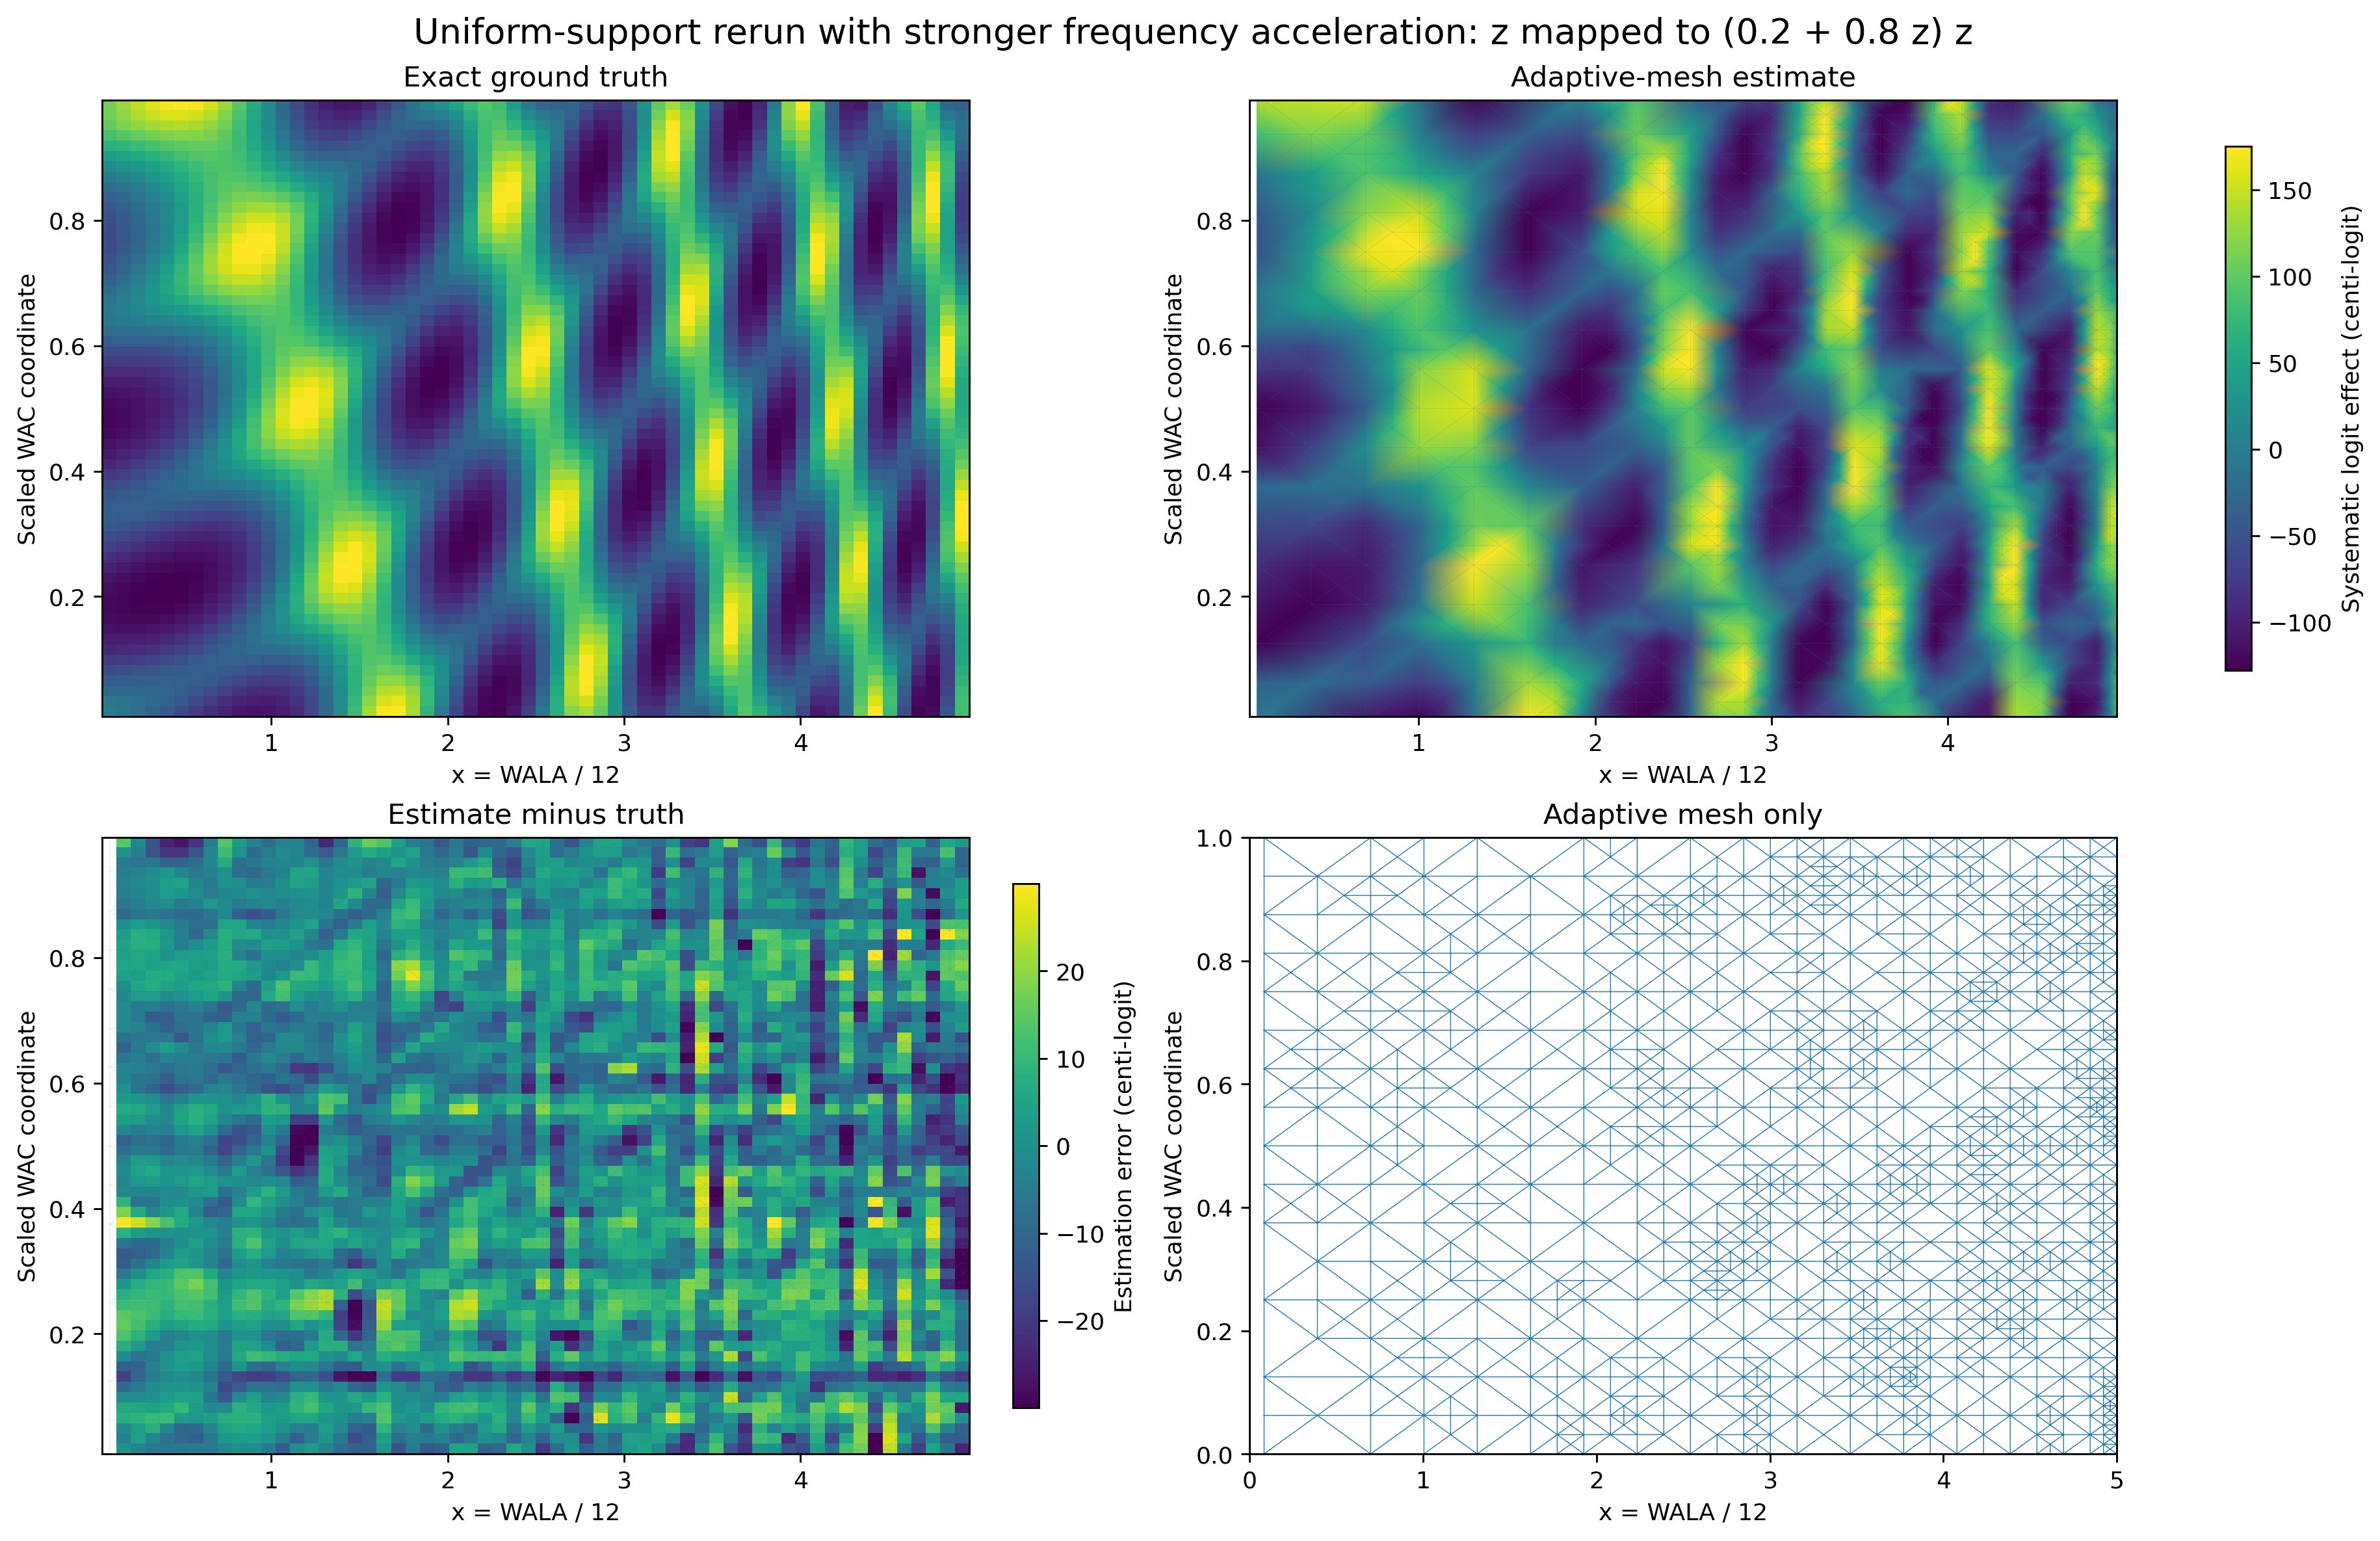
\includegraphics[width=\textwidth]{fig24_uniform_warped_benchmark.png}
\caption{Controlled uniform-support benchmark with increasing horizontal frequency.  The
panels show the exact truth, adaptive-mesh estimate, estimation error, and the final mesh.
The data cover the full WALA--WAC rectangle with zero attrition, separating geometric
adaptation from sampling-support artifacts.}
\label{fig:uniform-warped}
\end{figure}

\subsection{June 2026 Ginnie Mae fit on the log-odds scale}

The same estimator was applied to June 2026 Ginnie Mae single-family pool data using the same
constructed loan-count attrition proxy. Because there is no known ground-truth correction surface,
real-data diagnostics are reported on the proxy log-odds scale using information-weighted empirical
logits and held-out residuals; these are not SMM diagnostics.  The
full fit used 371,089 pools, 8,601 vertices, and 17,049 triangles.  The resulting geometry
is substantially more irregular than in the controlled benchmark because the empirical
WALA--WAC support and information density are highly nonuniform.

\begin{figure}[ht]
\centering
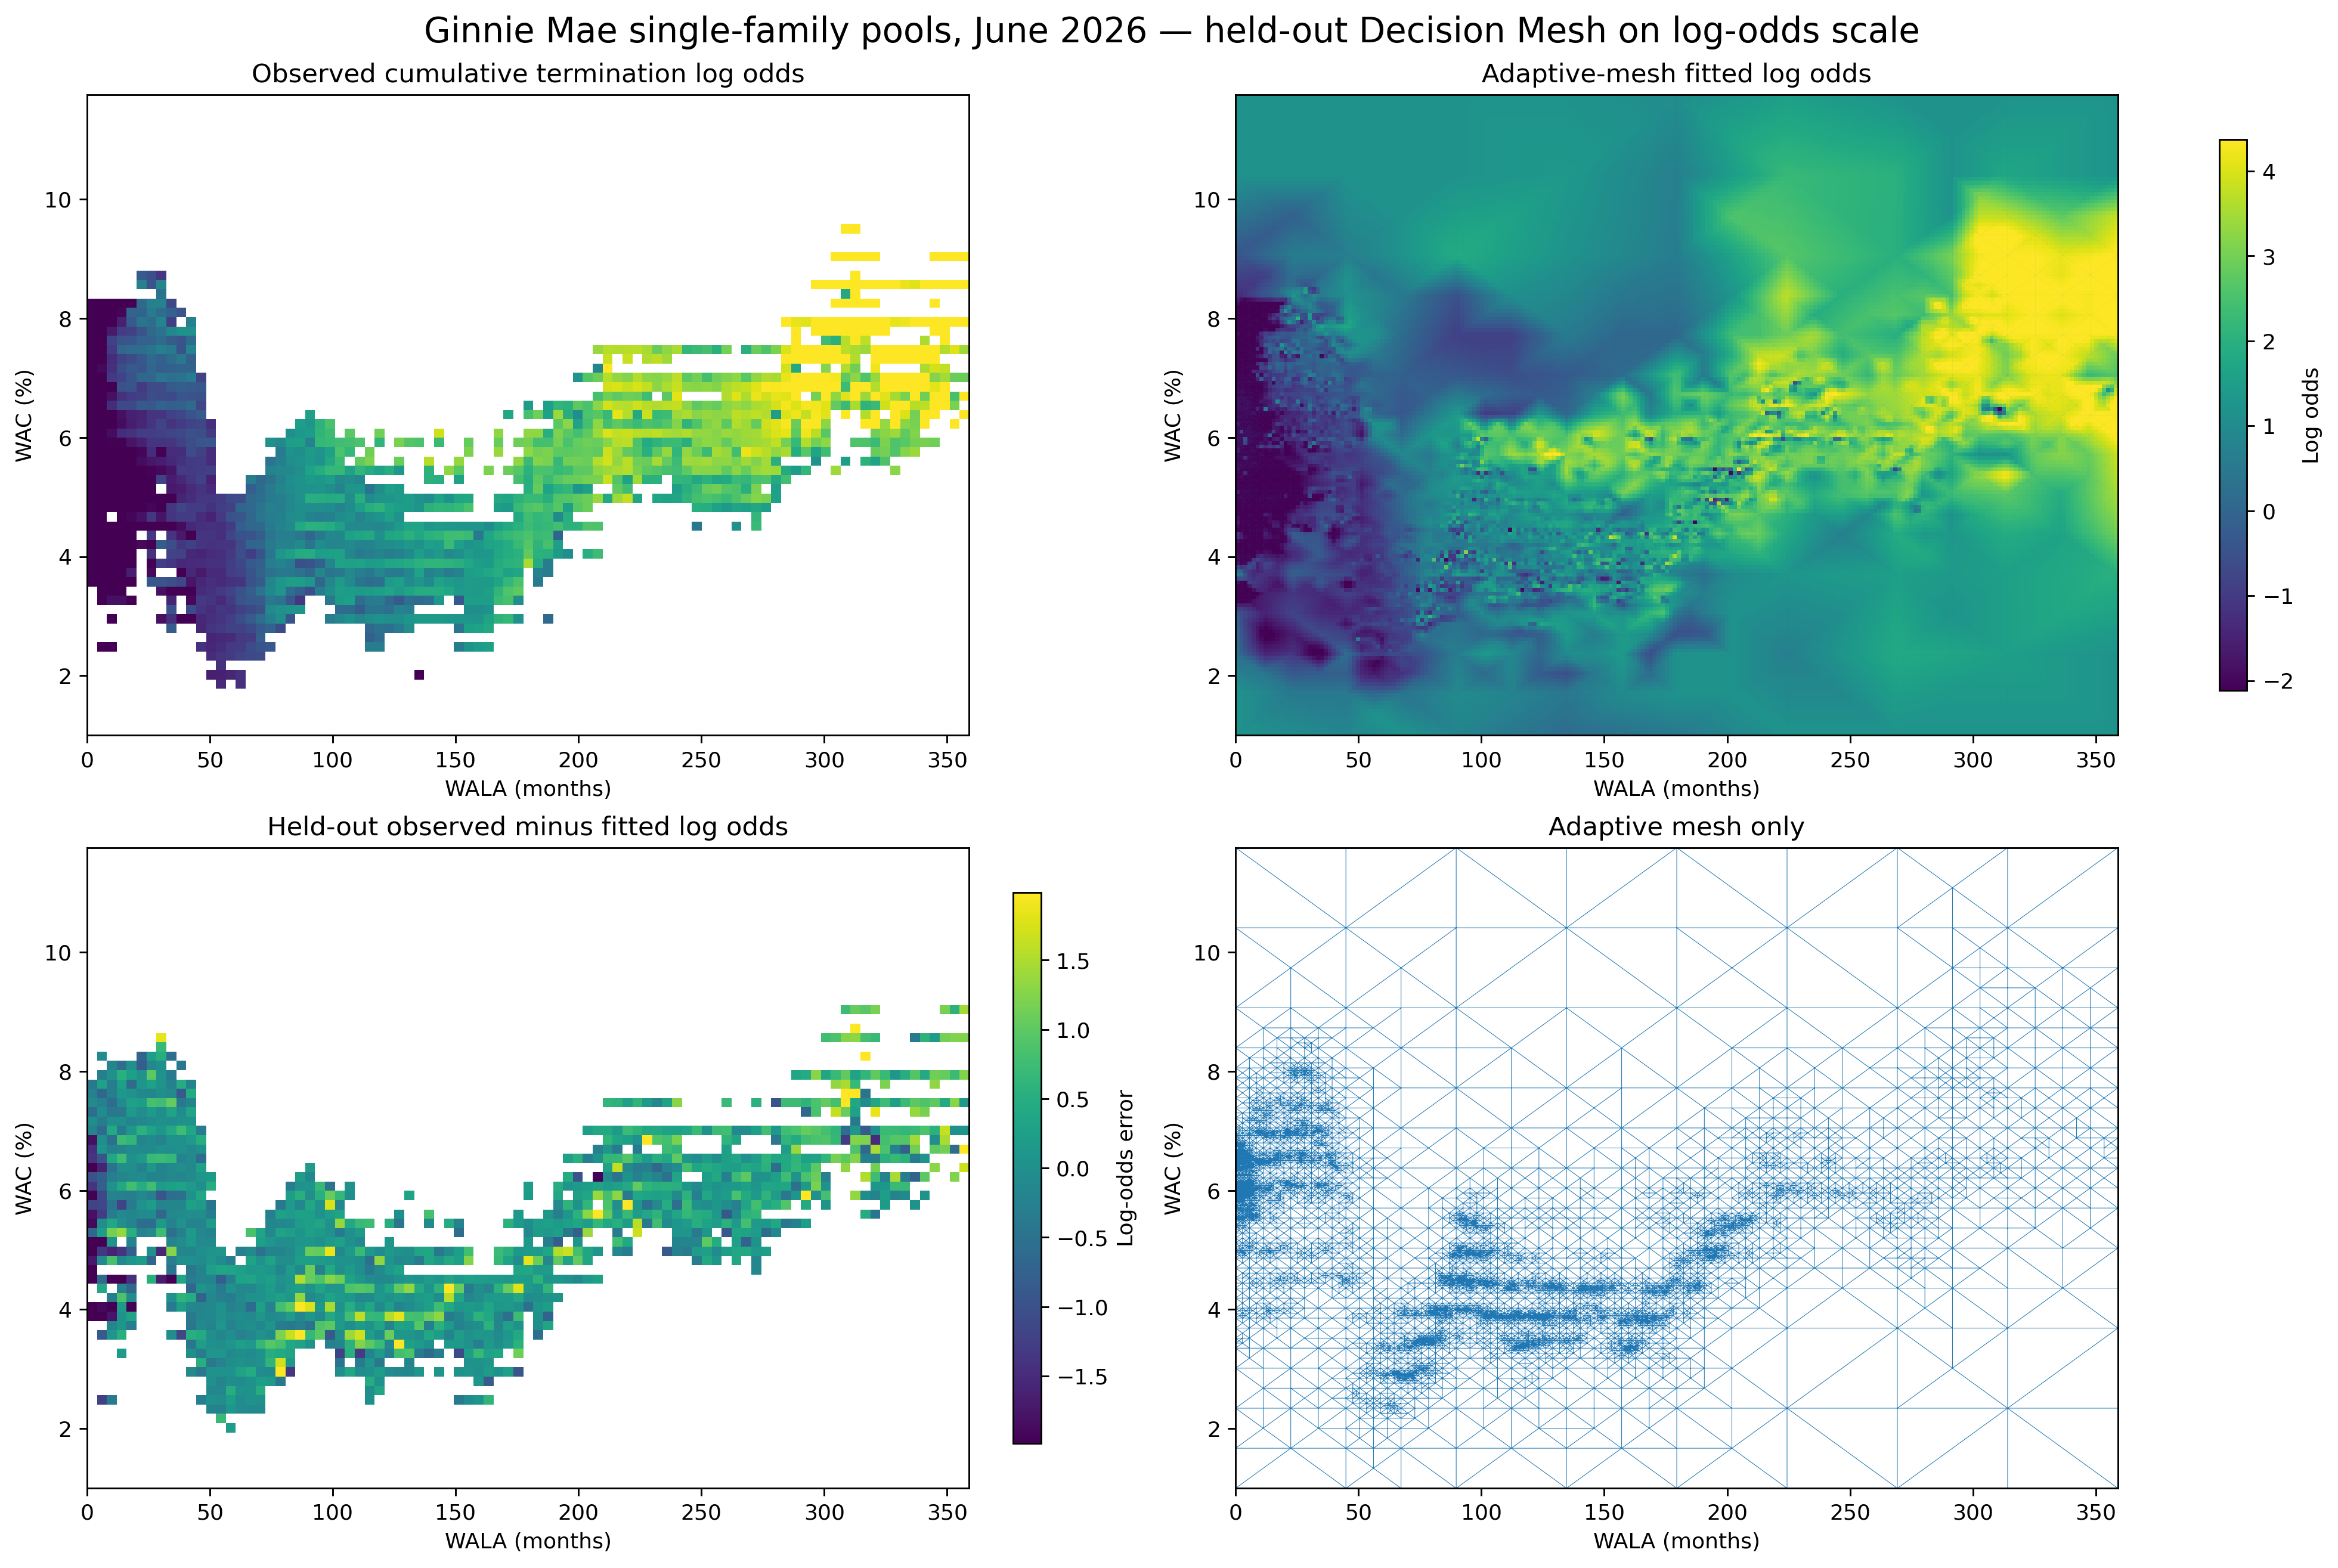
\includegraphics[width=\textwidth]{fig25_gnma_logodds.png}
\caption{June 2026 Ginnie Mae fit on the log-odds scale.  The panels show empirical log
odds, fitted log odds, held-out empirical-minus-fitted log odds, and the adaptive mesh.
Empirical logits use a Jeffreys $0.5$ correction to avoid infinities in saturated cells.}
\label{fig:gnma-logodds}
\end{figure}

\subsection{Evidence of undershrinkage after deep refinement}

The real-data mesh contains clusters in which triangle area becomes extremely small after
many successive refinements.  Several diagnostics indicate that at least some of these
clusters retain too much fine-scale variation.  First, held-out error is higher in the
finest triangle-area decile than at several intermediate resolutions.  Second, a
cross-fitted multilevel diagnostic compares the variation implied by the sequence of
hierarchical prior variances with independently realized variation over the final $k$
levels of the hierarchy.  For a suspicious central cluster the realized-to-implied
variance ratio was approximately
\[
 0.90,\ 0.94,\ 1.40,\ 0.35
\]
for one through four levels respectively.  Thus one-level behavior is not obviously
miscalibrated, while four consecutive levels collectively imply roughly three times the
variation supported by independent data.

Depthwise prior standard deviations in the same experiment became very large at
intermediate-deep levels, reaching roughly $1.9$--$2.1$ log-odds units at depths 6--7.
Turning on the existing admission-truncation correction improved held-out fit but drove
most deep prior scales to the lower floor, suggesting that the uncorrected estimator is
too permissive whereas the full correction is too aggressive.

\begin{figure}[ht]
\centering
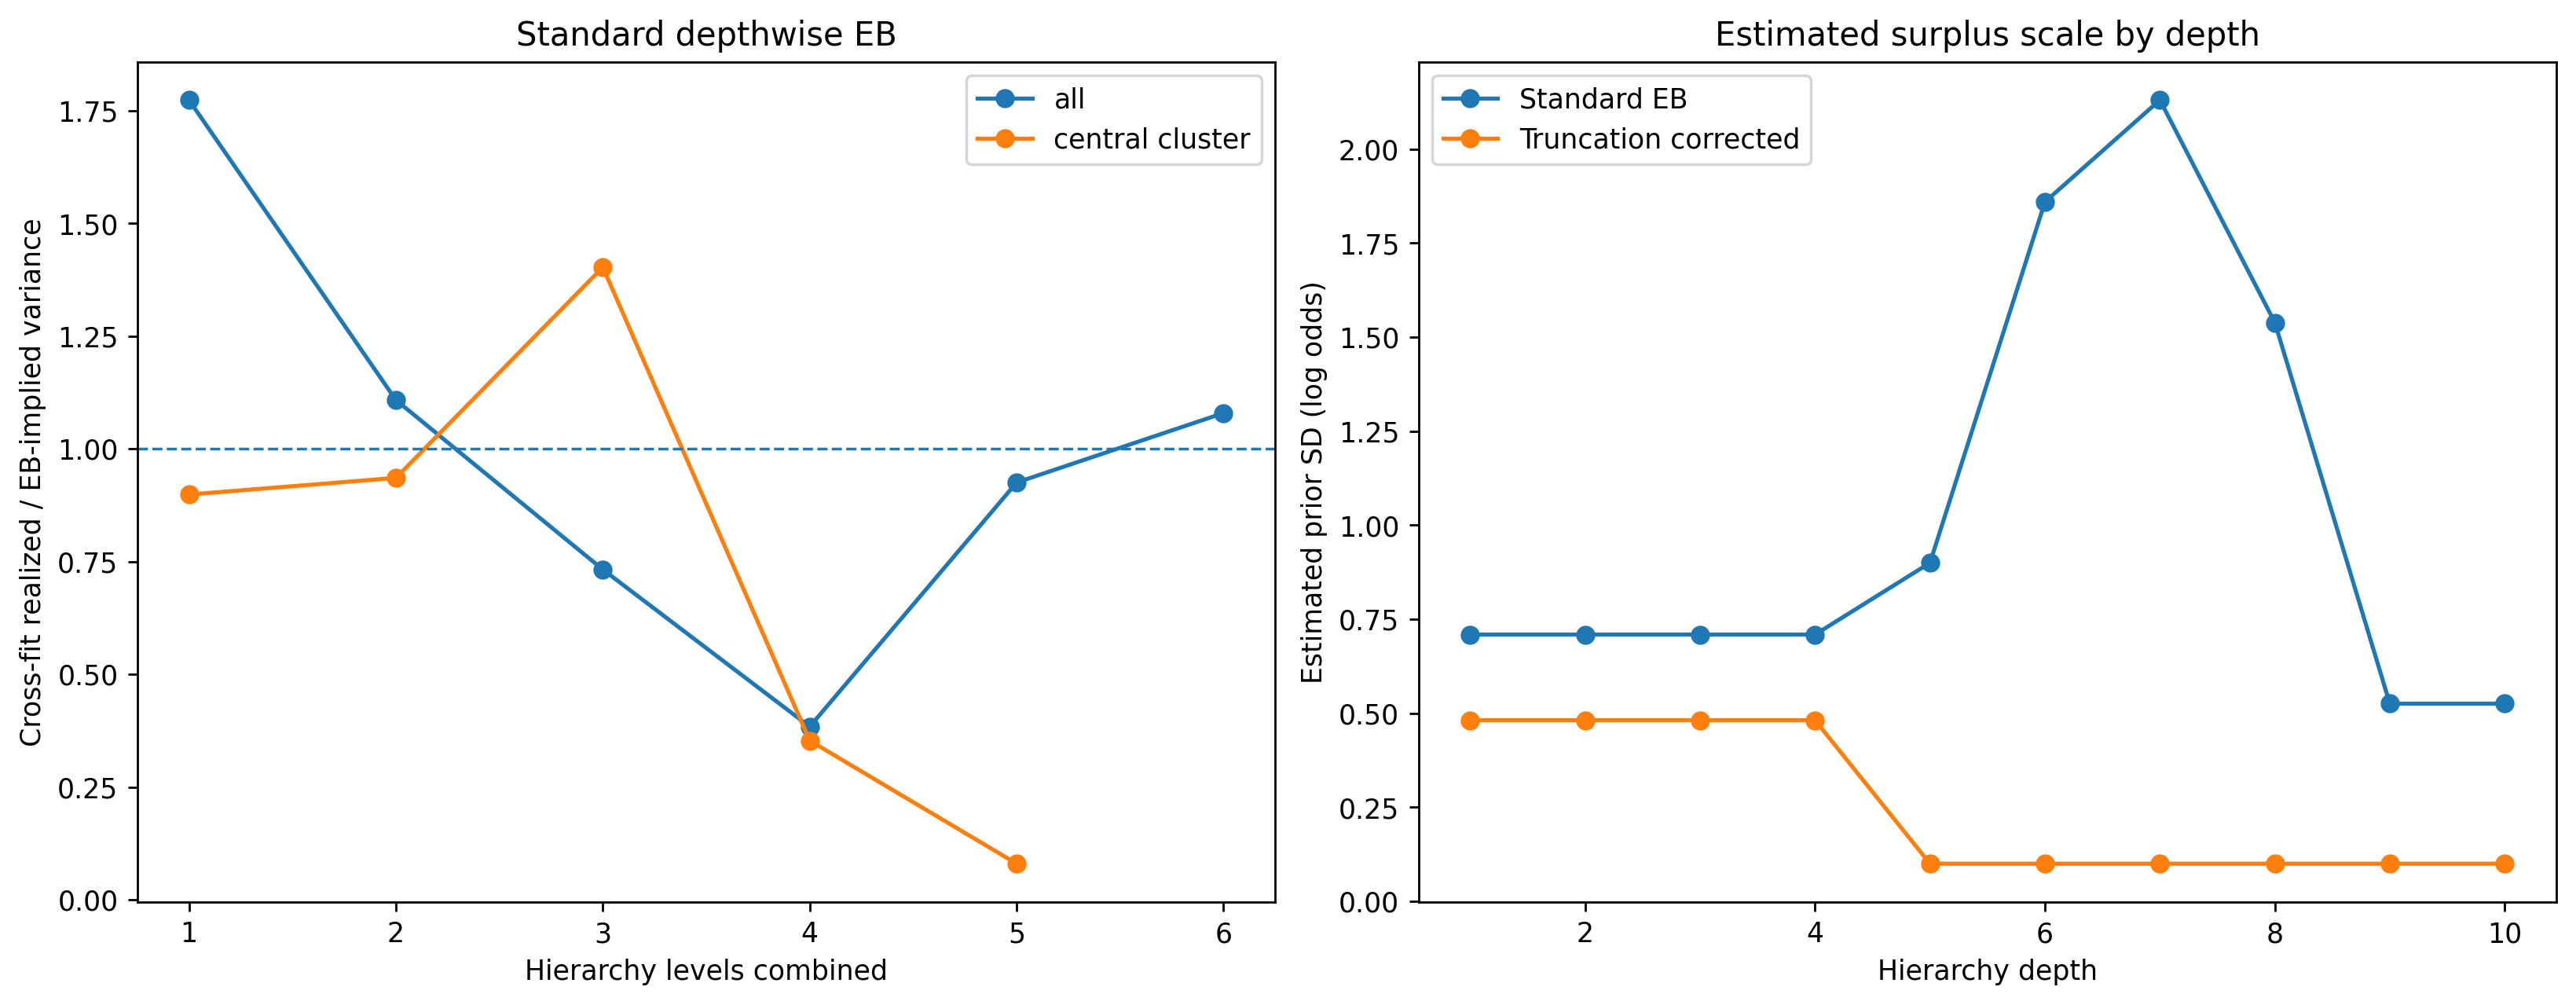
\includegraphics[width=0.94\textwidth]{fig26_multilevel_tau.png}
\caption{Multilevel hierarchical-variance diagnostic on a stratified Ginnie Mae sample.
Left: cross-fit realized variance divided by the variance implied by the estimated
hierarchical prior over multiple levels.  Right: estimated prior standard deviation by
depth under the ordinary and admission-truncation-corrected moments.  The ordinary
estimator permits excessive cumulative variation over several consecutive levels, while
the full truncation correction collapses deep scales toward the imposed floor.}
\label{fig:multilevel-tau}
\end{figure}

A direct manual ablation confirms that the smallest-triangle clusters contain removable
fine-scale variation.  Holding the geometry fixed, a local Laplacian smoothing step was
applied only to the finest 10\% of vertices.  On a stratified 80,024-row sample, the best
manual setting reduced held-out binomial deviance per pool from $19.29$ to $18.08$ overall.
Within the support directly affected by the smoothing, deviance fell from $53.50$ to
$23.64$.  The improvement is heterogeneous: some central regions did not benefit from the
same blanket smoothing rule.  The conclusion is therefore not that all deep refinement is
spurious, but that the current shrinkage can be insufficient in selected runaway branches.

\begin{figure}[ht]
\centering
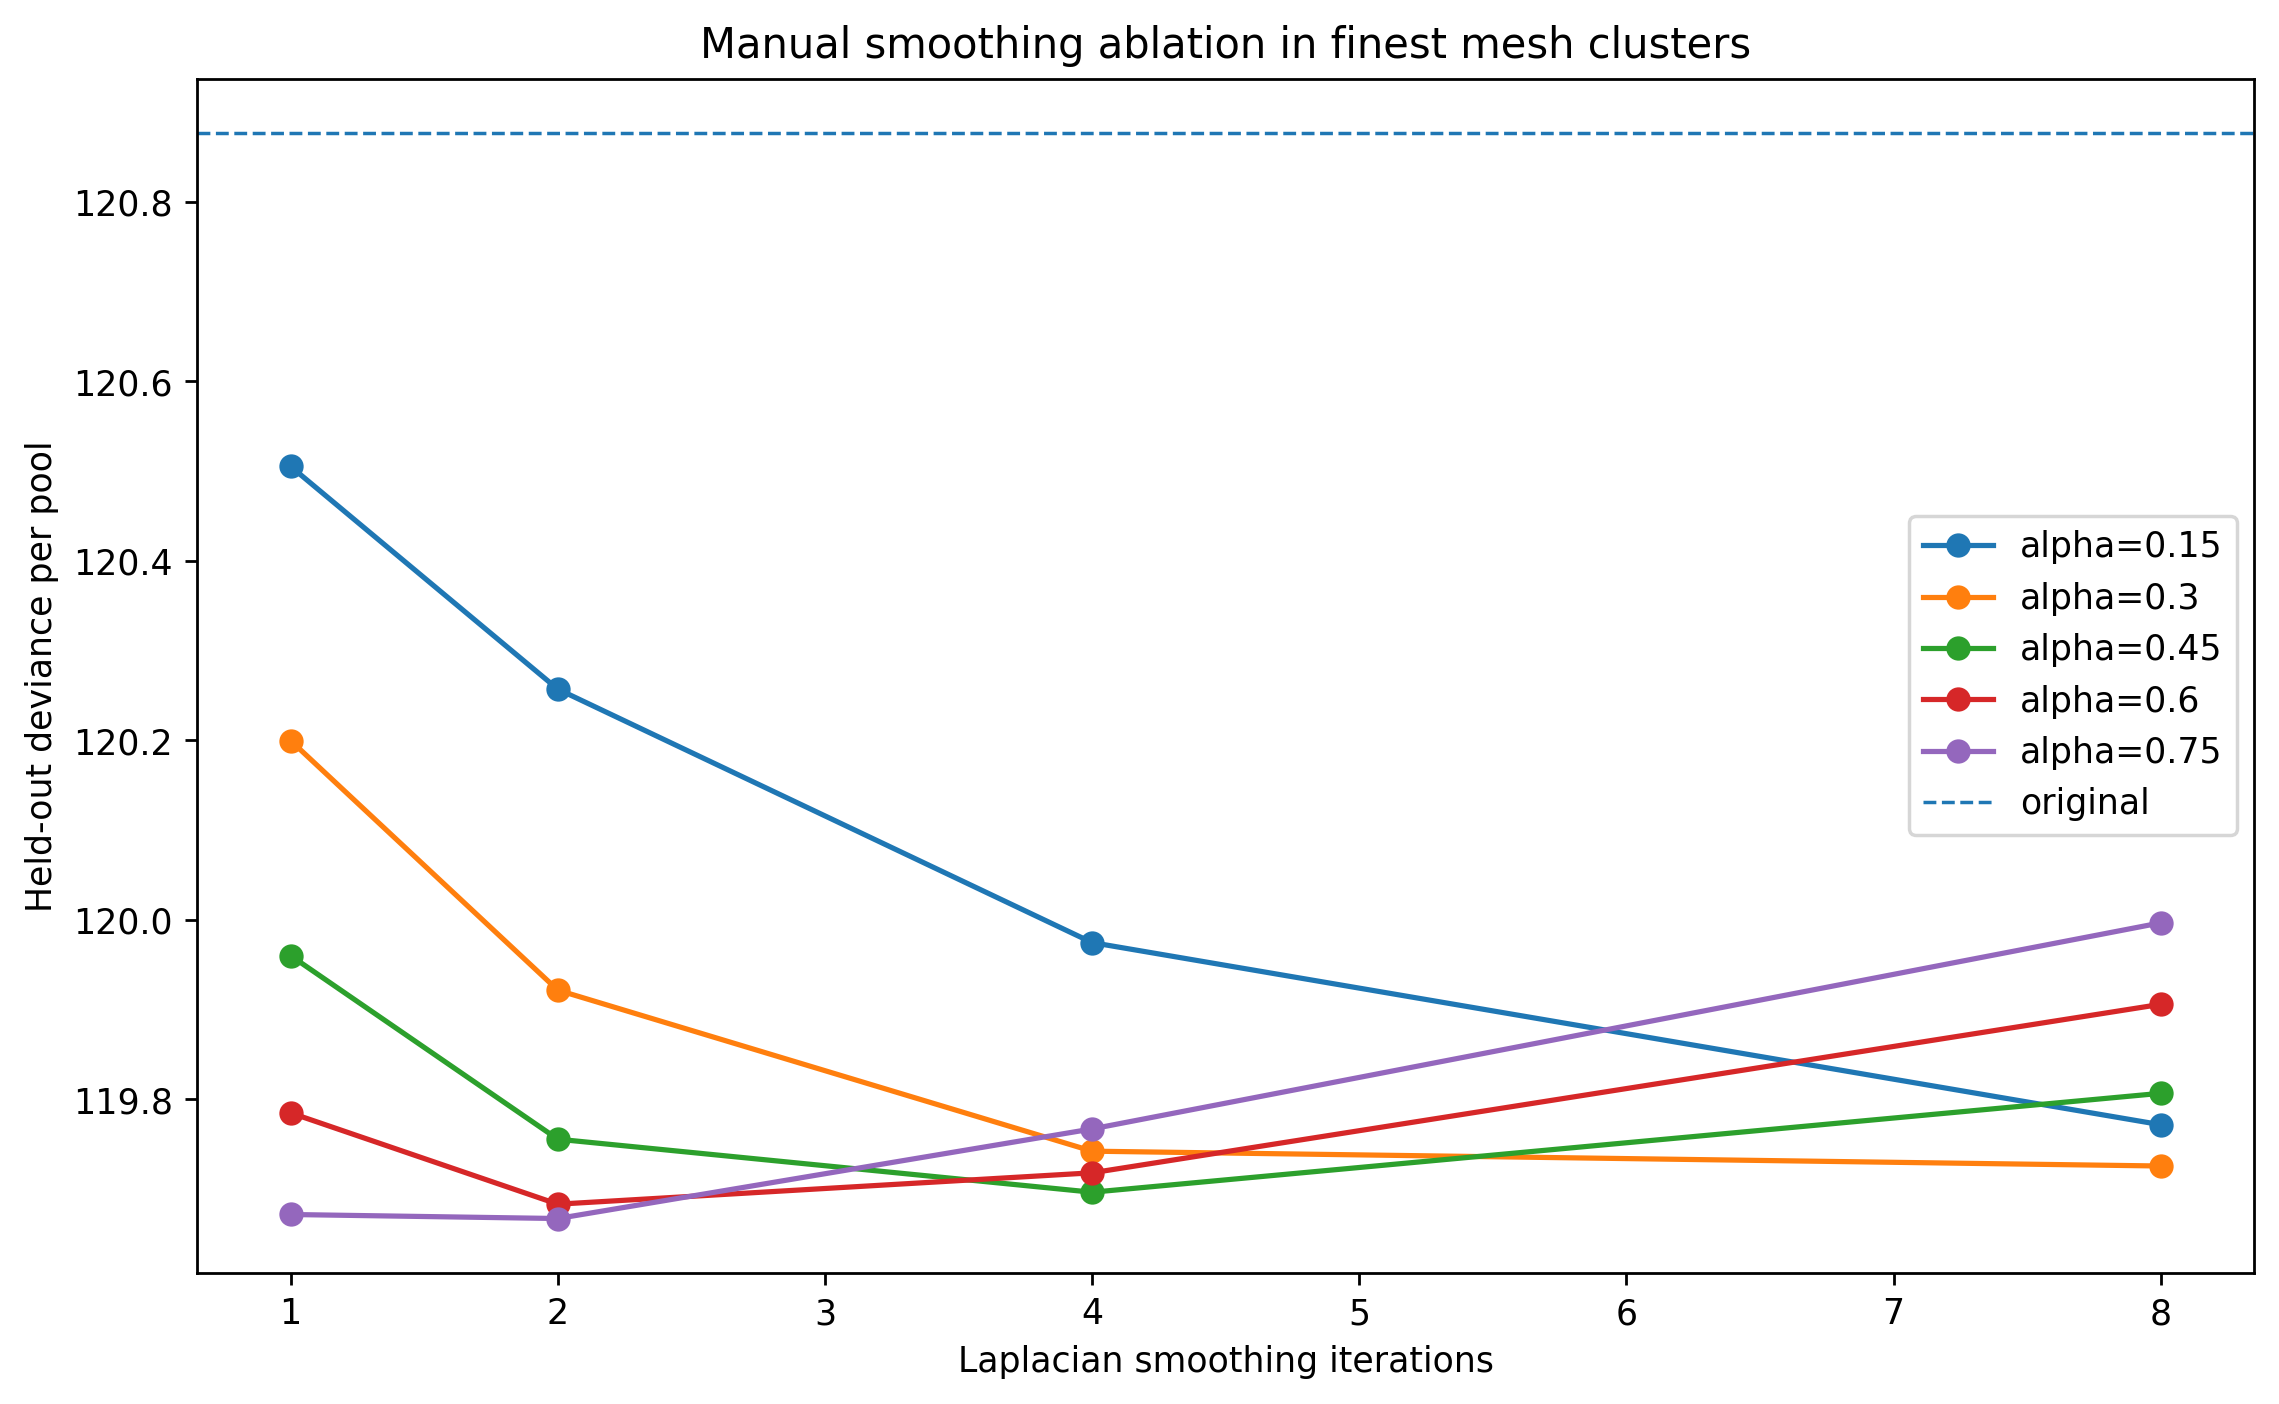
\includegraphics[width=0.86\textwidth]{fig27_manual_smoothing_ablation.png}
\caption{Held-out deviance under manual smoothing of only the finest mesh vertices.  The
ablation demonstrates that additional smoothing in selected deep clusters can materially
improve predictive likelihood, motivating a more selective empirical-Bayes calibration of
fine-scale branches rather than a global increase in regularization.}
\label{fig:manual-smoothing}
\end{figure}

\subsection{Focused diagnostic: WALA 100--150 and WAC 3.5--4.5}

A focused window at WALA 100--150 and WAC 3.5--4.5 contains 5,075 observations, 309 active
vertices, 123 gate-admitted vertices, and 678 intersecting triangles.  Its held-out
log-odds RMSE is $1.05$ with mean empirical-minus-fitted log-odds error $-0.18$.  The
hierarchical surplus magnitude does not decay with depth: median absolute surplus is about
$0.48$ at depth 7, $0.72$ at depth 8, $0.96$ at depth 9, and $0.87$ at depth 10.  All five
local depth-10 vertices are admitted.  This is consistent with a refinement branch that
continues to carry large coefficients after the mesh has become very fine.
These observations are resolved by the certified benchmarks of
Section~\ref{sec:certnull}: the deep admission \emph{count} in such
windows is reproduced on data whose truth is provably flat there (an
admission-side artifact of the conditional null under real-design density
and overdispersion), while the anomalous \emph{amplitude} decomposes into
mega-pool state masquerading as surface plus a residual genuinely sharp
component; the composite gate of Section~\ref{sec:nulls} removes the
manufactured population ($886\to2$ on the certified null) and the manual
smoothing ablation below is the crude form of the post-selection
re-shrinkage pass now implemented.

\begin{figure}[ht]
\centering
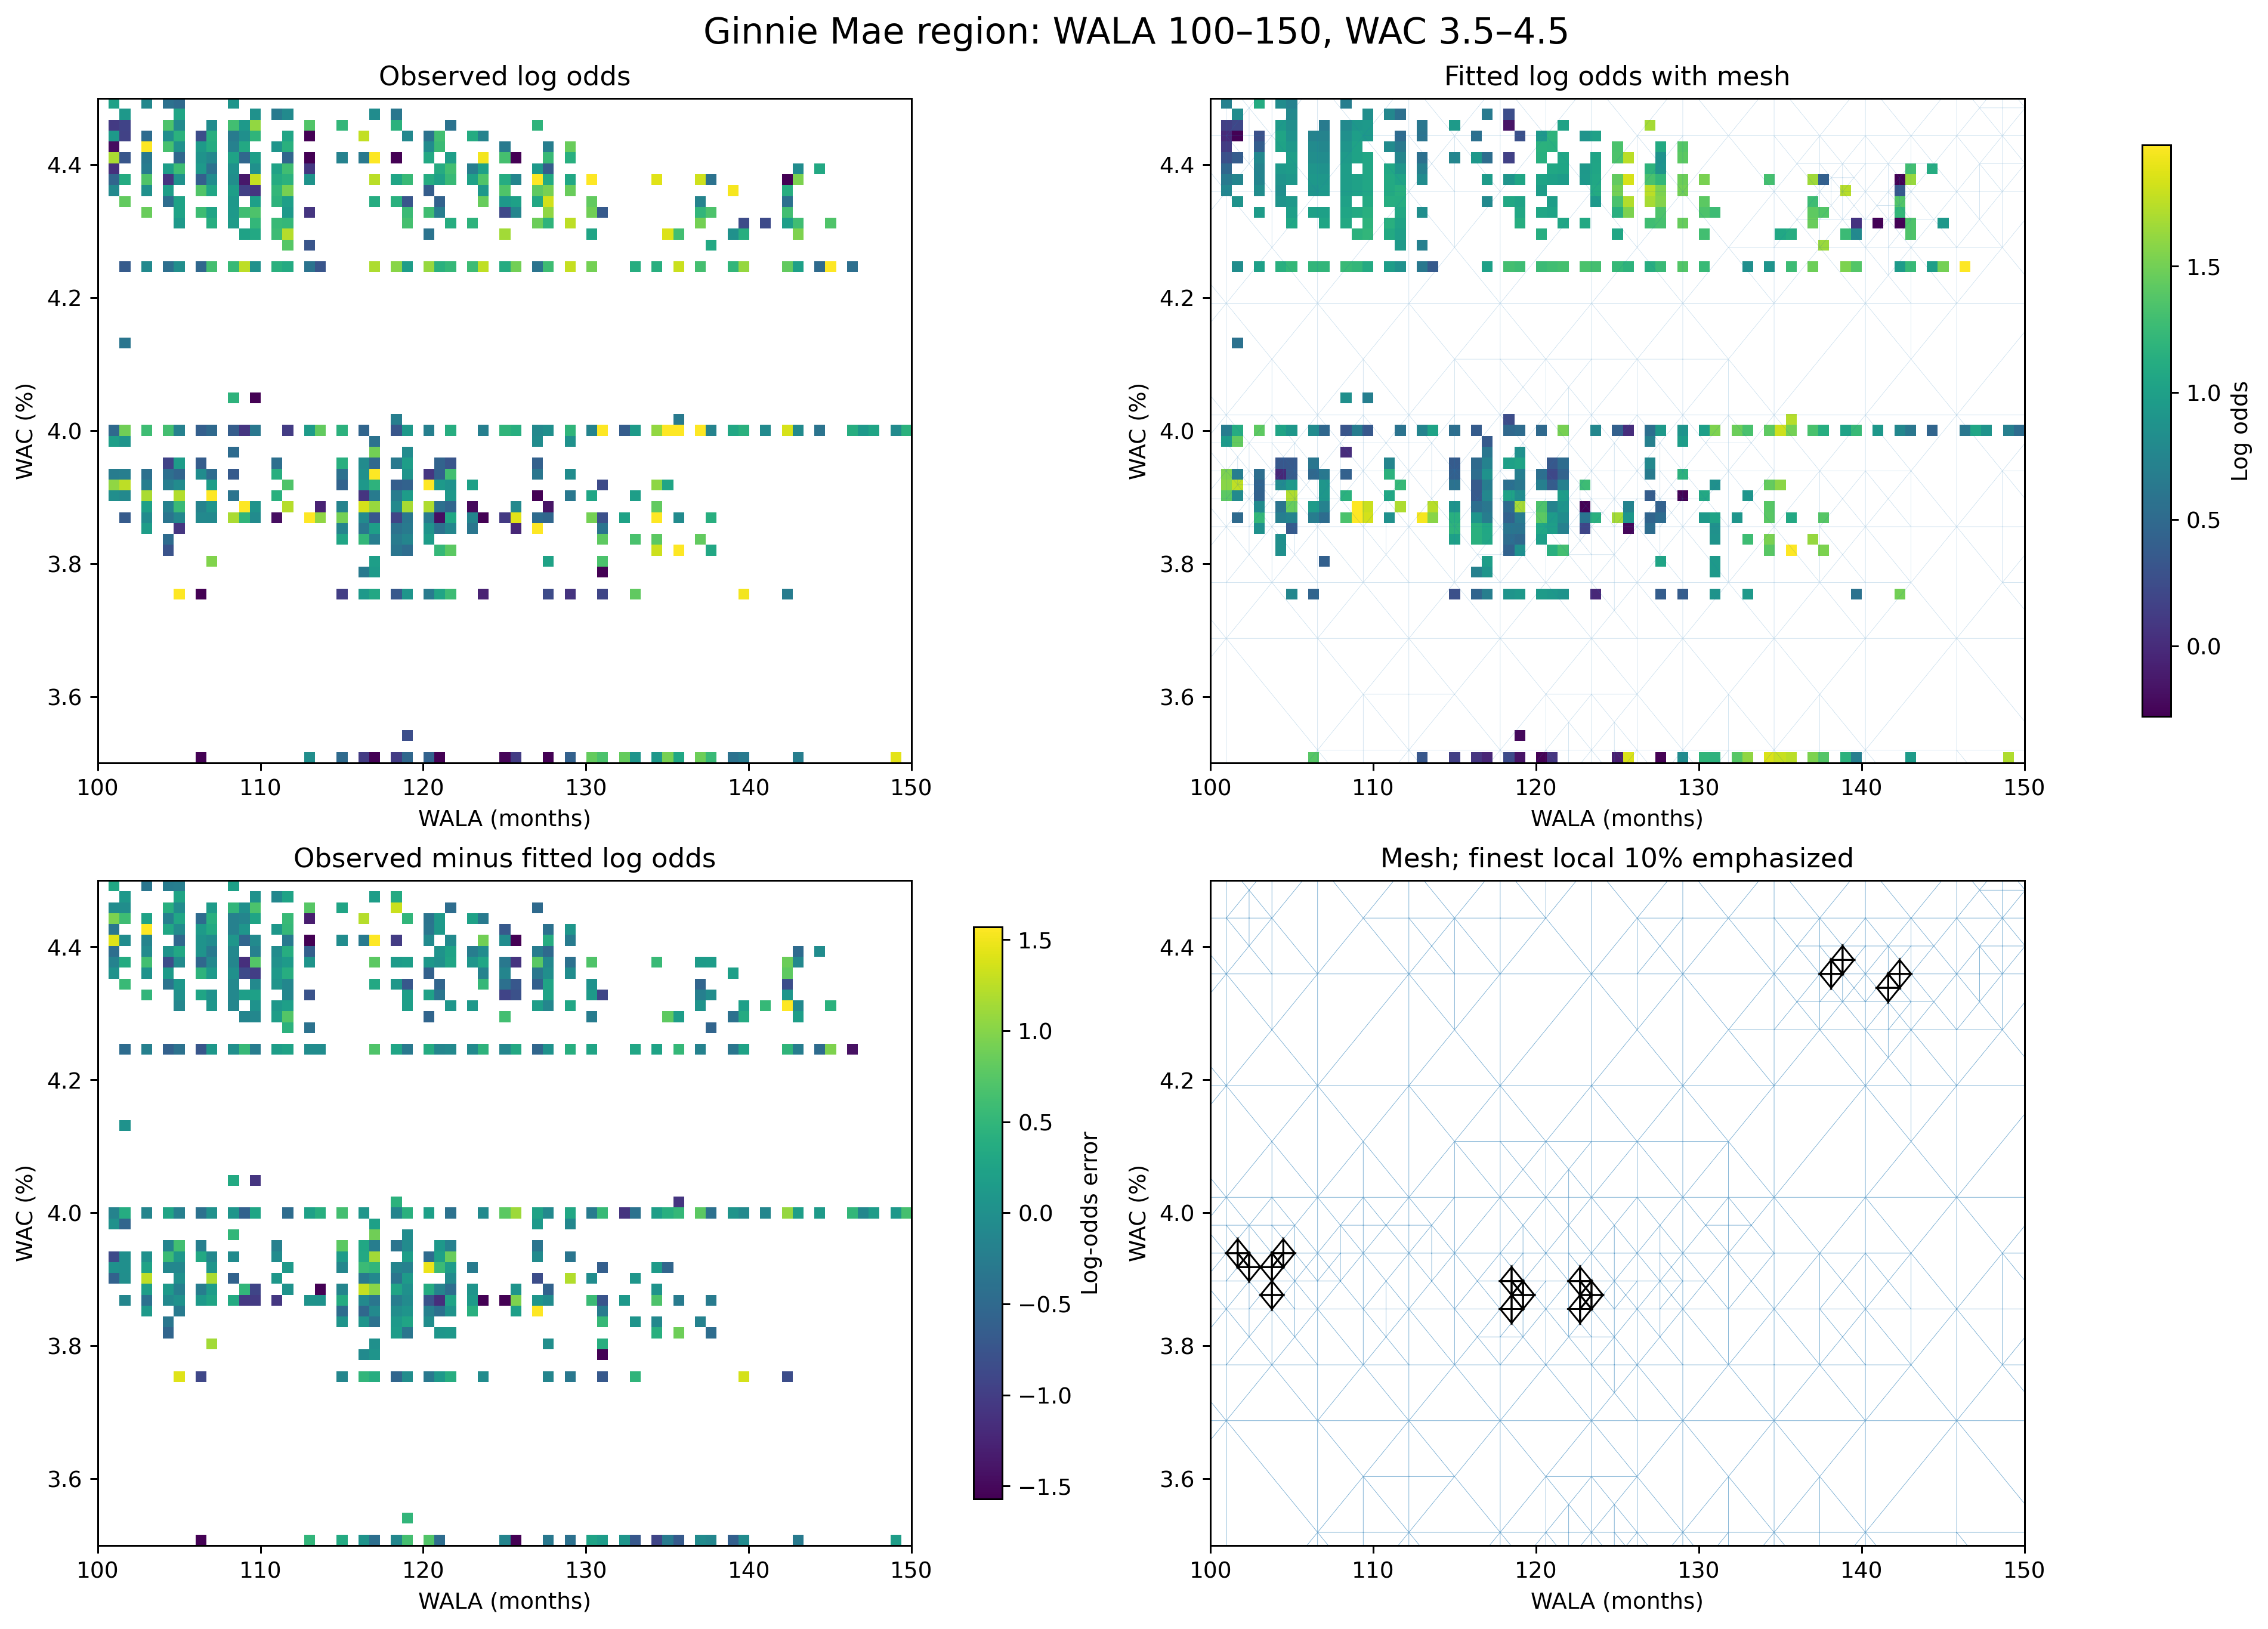
\includegraphics[width=\textwidth]{fig28_gnma_region_zoom.png}
\caption{Focused Ginnie Mae diagnostic for WALA 100--150 and WAC 3.5--4.5.  The panels
show empirical log odds, fitted log odds with the local mesh, held-out residual structure,
and the mesh with the finest local triangles emphasized.}
\label{fig:gnma-region-zoom}
\end{figure}

\begin{figure}[ht]
\centering
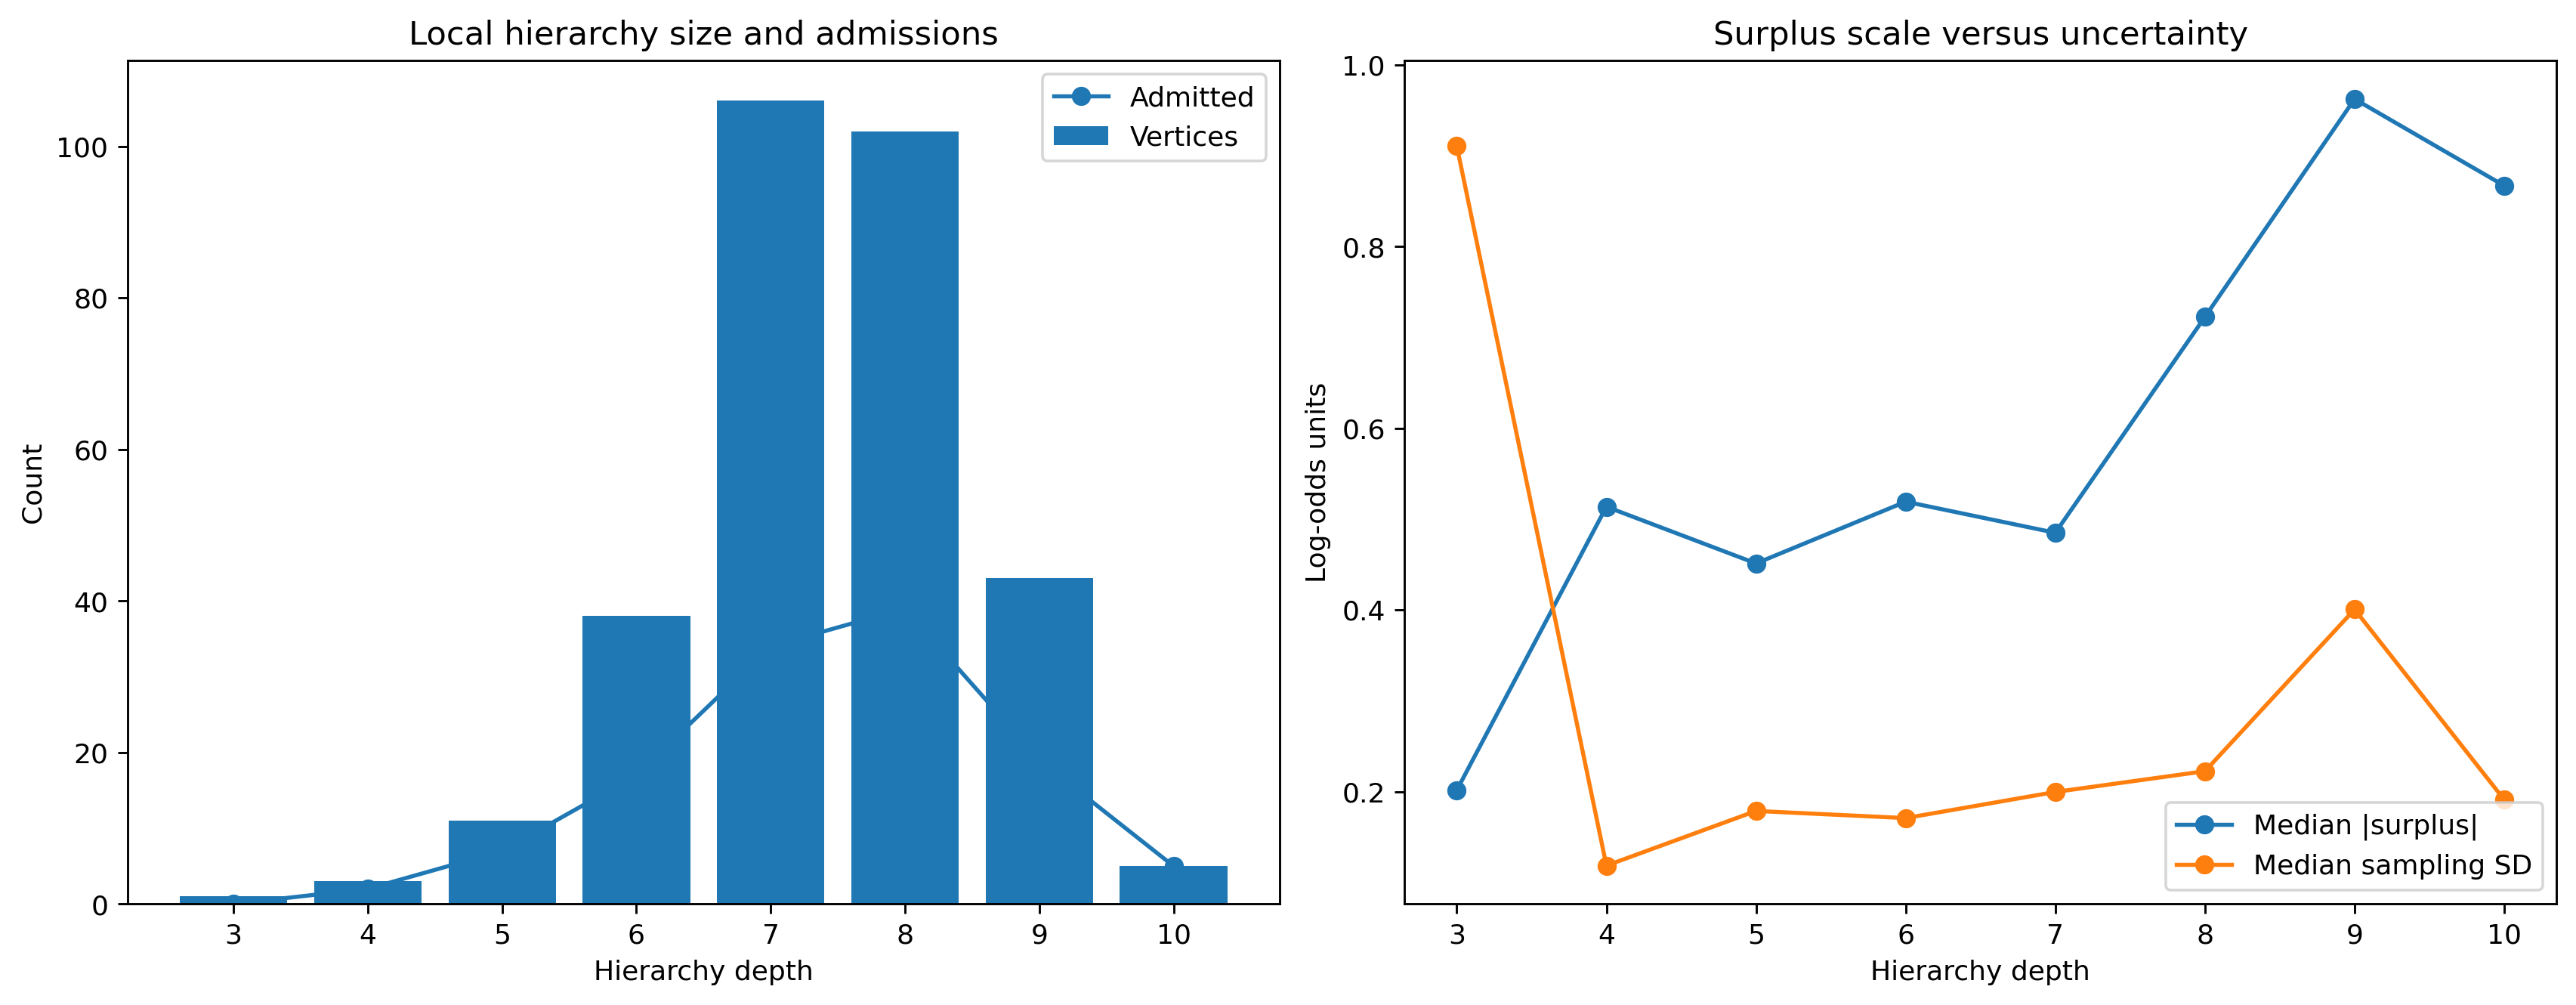
\includegraphics[width=0.88\textwidth]{fig29_gnma_region_depth.png}
\caption{Hierarchy diagnostics in the WALA 100--150, WAC 3.5--4.5 window.  The number of
admitted vertices remains substantial at deep levels and median surplus magnitude rises at
depths 8--10 instead of dying away.}
\label{fig:gnma-region-depth}
\end{figure}

\paragraph{Current recommendation.}
For the adaptive release path, retain the exact coupled mesh with quadratic inherited-child
shrinkage rather than a blanket increase in the fine-scale penalty. A first broad
split-genealogy local-branch EB model remains rejected: it improved some suspicious clusters but
overshrank healthy regions and worsened aggregate held-out performance. That result does not extend
to all geometric pooling. Final-geometry patch variance sharing is modestly positive, and nested
crossed covers produce a larger, stable frozen-topology improvement as documented in
Section~\ref{sec:geometry-eb}. The open methodological problem is to integrate that function-level
geometry jointly with the mesh and estimate its precision from conditional information, while
regularizing only branches whose multilevel implied variation is unsupported.


\section{Certified null benchmarks}\label{sec:certnull}
The certified-window instruments separate predictive fit from false geometric discovery. They use
the exact real design but replace the truth inside a declared window by a function whose deep
hierarchical surpluses are negligible. A deep admission in the interior is therefore false by
construction. This section reports two different statuses: the legacy gate has passed these
instruments; transfer of the same claims to the exact-solver gate has not.

An earlier matched-null claim was retracted on a ground worth stating as a result: matched fidelity
and sharp-null-everywhere are incompatible. The legacy boundary profile carried depth-8-scale
curvature near WALA $0$. The current April proxy audit additionally marks WALA~0 as measurement contaminated, so no present certification claim uses that region. The standing
instruments instead certify
$W=\mathrm{WALA}[80,200]\times\mathrm{WAC}[3,6]$ on the exact April 2026 design.

\subsection*{Legacy certified results}
\textbf{v3.} Truth is a realistic nine-parameter log-age polynomial everywhere except $W$, where it
is that polynomial's own quadratic fit with a cosine taper. The maximum true hierarchical surplus
in the window interior is $1.65/0.77/0.36$ centi-log-odds at depths $8/9/10$, two orders of magnitude
below admission scales. The legacy baseline gate produced $886$ certified-false deep faces; the
analytic composite gate produced $2$.

\textbf{v4.} The mean is the same, but the noise includes the measured size-dependent pool variance,
small-pool heavy tails, real issuer assignments with $0.09$ issuer variance, diversified
multi-issuer pools, and a shipped known $n_{\mathrm{eff}}$. The legacy baseline produced $997$
certified-false faces; the analytic composite gate produced $7$ and the permutation gate $6$. The
$2\to7$ change is the expected issuer-clustering attack: co-located pools sharing an issuer draw
replicate like surface unless effective replication is priced over issuers rather than pools.

\subsection*{Exact-score transfer experiment B3: failed}
The B3 transfer froze the signed-root score definition \eqref{eq:exactgain} and attempted to
standardize it by a candidate-specific sandwich factor,
\begin{equation}\label{eq:b3score}
z_v^{B3}=\frac{r_v}{(\widehat{\mathrm{sd}}_{\delta,v}/100)\sqrt{I_v}},
\end{equation}
with the remaining family-level location and scale estimated by central matching. On an independent
complete-null simulation, the first exact-score rounds were close to unit scale (stage 1 mean
$0.013$, sd $1.001$; stage 2 mean $0.012$, sd $0.992$), and the run ended with four false
admissions. Prediction on the original and eruption-seed splits also remained stable.

The certified windows nevertheless rejected the proposal. An initial wiring omission set the
pool-noise variance to zero and reproduced the old failure almost exactly: v3 had $992$ and v4 had
$982$ certified-false faces. After correctly pricing the declared composite variance $0.35$, v3 fell
to $80$ under the standard stage-0 policy and $75$ when stage 0 also used the exact score, still far
from the predeclared target near $2$. The corrected v4 run generated a large adaptive workload and
did not complete within the run budget; its trajectory was not approaching the required $3$--$7$
range. B3 is therefore not accepted, and no legacy certification claim transfers to the exact gate.

The failure is informative. The exact one-dimensional objective and its signed gain pass their local
invariants, but a single global empirical-null/prefix rule can admit null candidates inside $W$ as
passengers behind strong candidates elsewhere or can pool together fit states with different residual
laws. The next calibration must be local to the candidate's held-out evidence or otherwise condition
on the adaptive state.

\subsection*{Conformalized held-out certification: proposed}
A conformal construction is possible, but a naive pointwise conformal interval is not enough. Standard
split-conformal coverage is marginal for a future observation; it does not by itself control an
adaptively generated family of local surface hypotheses. A valid version must separate hypothesis
generation from calibration and preserve the pool/issuer dependence structure.

One concrete design is:
\begin{enumerate}[leftmargin=2em,itemsep=2pt]
\item Split observations by exchangeable pool or issuer blocks into a \emph{construction} sample and
a \emph{calibration} sample. Build the current mesh, fit the null surface, and freeze the candidate
set using only the construction sample.
\item For candidate $v$, estimate its direction and amplitude $\hat a_v$ on the construction sample.
On each calibration block compute the held-out directional log-likelihood increment
\[
A_{bv}=\sum_{i\in b}c_i\left\{\ell_i(\eta_i+X^H_{iv}\hat a_v)-\ell_i(\eta_i)\right\}.
\]
This prevents the candidate from choosing its direction on the same outcomes used to certify it.
\item Within prespecified exchangeability strata (pool size, fitted hazard, issuer structure, and
possibly stage/depth), permute residual bundles among geometric slots or use leave-one-block-out
nonconformity ranks. The conformal/permutation p-value is
\[
p_v=\frac{1+\#\{b:T^{(b)}_v\ge T^{\mathrm{obs}}_v\}}{B+1},
\qquad T_v=\sum_b A_{bv}.
\]
Equivalently, invert the test to obtain a conformal interval for the held-out gain or coefficient and
admit only when the interval excludes zero in the construction-sample direction.
\item Apply a multiplicity rule to the frozen family. Ordinary BH requires its usual dependence
conditions; blockwise permutation p-values or e-values with e-BH are safer when neighboring
candidates overlap. Cross-fitting can rotate construction and calibration folds to recover power
without reusing a candidate's own calibration outcome for its direction.
\end{enumerate}

This is best viewed as a conformalized version of the existing permutation null, with the important
addition that evidence is evaluated out of sample. It offers finite-sample validity under the stated
block exchangeability, but not assumption-free validity: calendar shocks, nonexchangeable issuer
formation, and adaptation after seeing calibration outcomes would break the guarantee. The v3/v4
windows provide the predeclared falsification suite for this proposal before any real-data adoption.


\subsection*{Complete-null comparison and sequential diagnosis}
A later audit separated the certified smooth-window question from a genuine complete null.  Both
complete-null designs reuse the Ginnie covariates and exposures but set the spatial correction to a
constant.  In the clean version the only randomness is binomial; in the matched heavy-tail version
pool effects are drawn from the same four size-stratified two-component law supplied to the
histogram gate.  Ten frozen seeds were run for each design.  The clean null stopped at the root mesh
in every seed: no admitted free coefficients, no depth-$\geq 8$ faces, and fitted spatial rms
$0.37$ centi-log-odds.  The matched heavy-tail null admitted an average of $2.4$ free coefficients
(median $1$, range $0$--$11$), admitted at least one coefficient in $6/10$ runs, produced an average
of $9.4$ depth-$\geq8$ faces, and left $8.09$ centi-log-odds of fitted spatial rms.  Thus ordinary
binomial null testing is not the difficulty; the remaining failure is specific to lumpy pool
heterogeneity and the adaptive reuse of its realized spatial pattern.

The certified v3 instrument is not a complete null.  It contains a legitimate quadratic trend in the
window and certifies only that deeper nonquadratic surpluses are negligible.  Under the deterministic
histogram gate, v3 produced $259$ admitted free coefficients overall and $14$ coefficient centers in
the window, all at hierarchical depths $4$--$5$; none was a depth-$\geq8$ free coefficient.  The
same run produced $35$ area-depth-$\geq8$ faces and approximately $5.65$ centi-log-odds of
nonquadratic fitted texture after removing the best quadratic.  The historical face count therefore
mixes legitimate low-order fitting, NVB closure, and false fine-scale texture.  It remains a useful
end-to-end geometry diagnostic, but it is not by itself candidate FDR after geometric existence and
statistical freedom have been separated.

The complete-null failure was then traced round by round.  The heavy-tail runs execute many adaptive
candidate-family tests; problematic seeds had $18$--$24$ rounds, with six to nine rounds containing
at least one rejection.  At the initial root family, only two of ten seeds rejected anything (six
candidates in one seed and one in another), which is not by itself a precise rejection of a nominal
$q=0.10$ all-null family with only ten repetitions.  Once a coarse false split is admitted, however,
the same realized pool anomaly changes the fit, generates descendants, and receives repeated
opportunities to be selected.  The final admission counts $11,0,5,0,2,0,1,0,1,4$ show this branching
pattern.  The failures are not confined to one-pool stars: among the $24$ admitted coefficients the
median variance-effective pool count was about $55$ and the median fourth-moment effective count
about $21$.  Increasing explicit mixture enumeration from eight to fourteen dominant contributors
left the problematic admission counts unchanged, so truncation of the deterministic histogram
convolution is not the leading error.

The current diagnosis is consequently two-part.  First-round histogram p-values are mildly
anti-conservative in their extreme tail under the lumpy law.  More importantly, per-round BH at a
fresh $q$ does not provide whole-run control for a data-adaptive branching dictionary.  The relevant
null distribution after the first split is selection-conditioned,
\[
 \mathcal L(U_v\mid\text{the current mesh was selected from the same realization}),
\]
not the marginal histogram law used at the root.  The next falsification suite therefore has three
arms: (i) a one-family heavy-tail null over at least $100$ frozen seeds; (ii) a frozen-dictionary
repeated-refit experiment; and (iii) the full adaptive run.  Their differences isolate marginal tail
calibration, refitting reuse, and descendant generation.  A plausible repair is branchwise or
sequential error spending, in which a root branch receives a fixed budget and descendants inherit
subdivisions of that budget rather than receiving a fresh $q=0.10$ family at every generation.  This
proposal is not yet implemented or certified.

\subsection*{Pooled-permutation admission gate: implemented experimental audit}

A separate implementation follows the candidate's own pool contributions
rather than importing a parametric pool law. Under a star-level null, residual
score contributions are permuted across the geometric hat-column slots. The
prototype computes the first three exact permutation moments, generates 32
deterministically seeded permutation draws per candidate, standardizes each
star by its own moments, pools the residual null shape across stars in bands of
star size, and applies direct BH. A commit-time support check enforces
$K_{\mathrm{eff}}\ge4$ in the best-controlled configuration. This is not yet
the proposed deterministic double-saddlepoint implementation, and the code is
shipped only as an experimental branch.

The null results are much stronger than the legacy gate. Across 34 frozen
complete-null datasets on the real Ginnie design, the shipped gate averaged
17.50 false admissions in a three-round battery and admitted in all 34 runs;
the permutation-BH rule with $K_{\mathrm{eff}}\ge4$ admitted none. Under full
adaptation, the shipped mean increased to 121.94 false admissions (maximum
1{,}001), whereas the permutation rule again admitted none. Raising the
support floor without permutation calibration did not explain the result: the
shipped gate with $K_{\mathrm{eff}}\ge4$ averaged 29.24 admissions in the
three-round battery.

\begin{figure}[H]
\centering
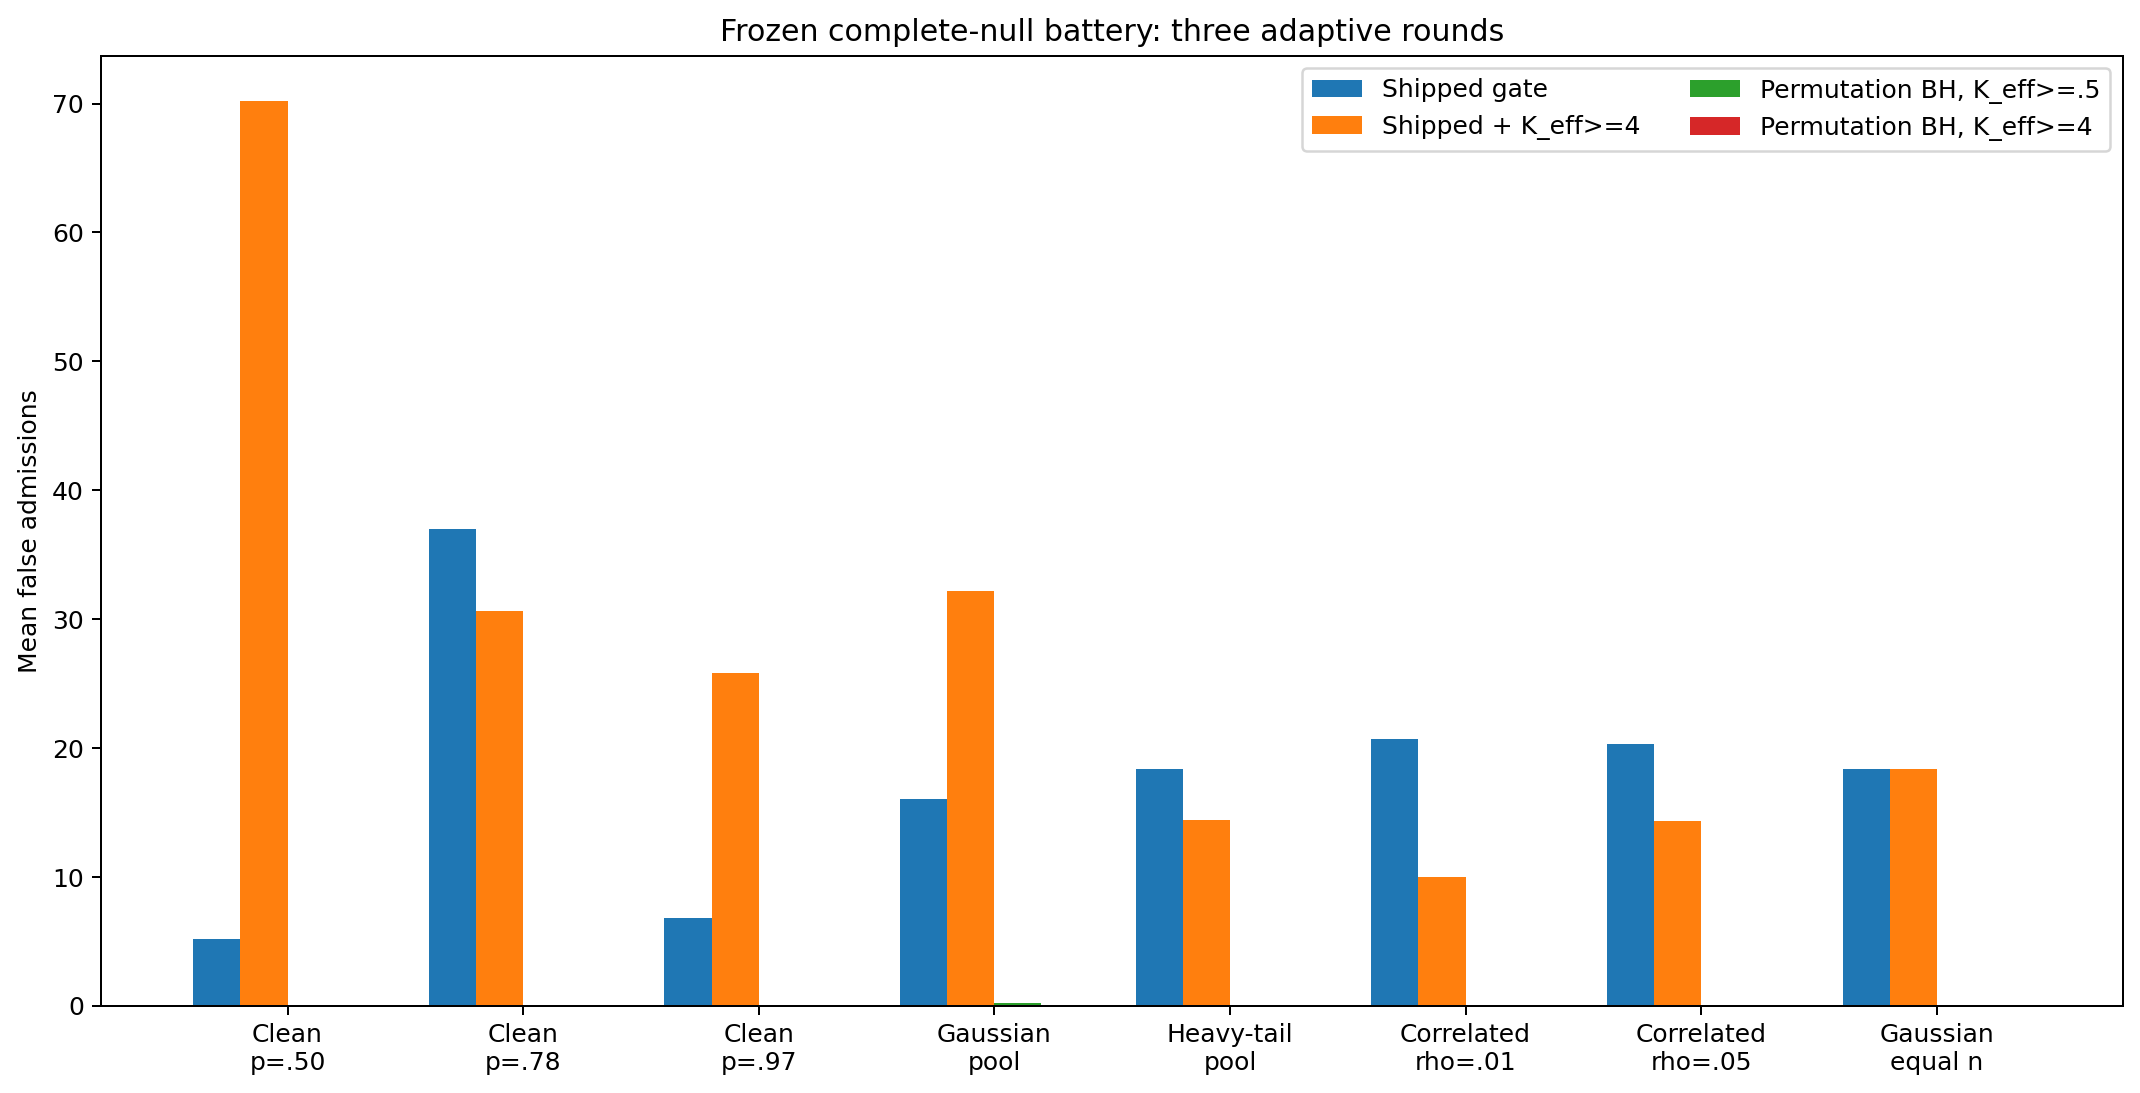
\includegraphics[width=0.94\linewidth]{permutation_null_battery.png}
\caption{Frozen complete-null battery under three adaptive rounds. The direct
pooled-permutation BH gate removes the broad false-admission failure across
clean, Gaussian-pool, heavy-tail, correlated, and equal-exposure scenarios.
The support floor alone is not sufficient.}
\label{fig:permutation-null-battery}
\end{figure}

The more informative tests retain genuine spatial signal outside a certified
quadratic window. Table~\ref{tab:permutation-certified} reports both the
original Gaussian-effect instrument and a new 20-seed heavy-tailed version
using the same 90/10 two-normal mixture with total variance 0.35 and a
wide/core variance ratio of 10.

\begin{table}[H]
\centering
\small
\caption{Certified-window results. ``Window admissions'' are admitted
coefficient centers inside the exactly quadratic window; ``deep faces'' are a
geometry footprint, not an FDR numerator. RMS and RMSE are centi-log-odds.}
\label{tab:permutation-certified}
\resizebox{\textwidth}{!}{%
\begin{tabular}{llrrrrr}
\toprule
Pool law & Gate & Total adm. & Window adm. & Deep faces & Window nonquad. RMS & Outside RMSE\\
\midrule
Gaussian & Shipped $q=.10$ & 110.0 & 8.2 & 73.8 & 4.69 & 13.47\\
Gaussian & Perm. BH $K_{\mathrm{eff}}\ge4$, $q=.10$ & 18.8 & 0.2 & 1.6 & 3.69 & 13.16\\
Heavy tail & Shipped $q=.10$ & 165.6 & 13.4 & 115.85 & 11.13 & 16.41\\
Heavy tail & Perm. BH $K_{\mathrm{eff}}\ge4$, $q=.15$ & 7.75 & 0.0 & 0.0 & 3.37 & 14.12\\
\bottomrule
\end{tabular}%
}
\end{table}

In the heavy-tailed instrument, the shipped gate entered the certified window
in 18 of 20 seeds and made direct deep admissions in seven. The
$K_{\mathrm{eff}}\ge4$, $q=.15$ permutation rule made no window admission and
no deep face in any seed, while also improving the fit to the genuine signal
outside the window. Increasing $q$ to .20 reduced outside RMSE only slightly
but reintroduced window admissions in four seeds; $q=.15$ is therefore the
best controlled point in that sweep.

\begin{figure}[H]
\centering
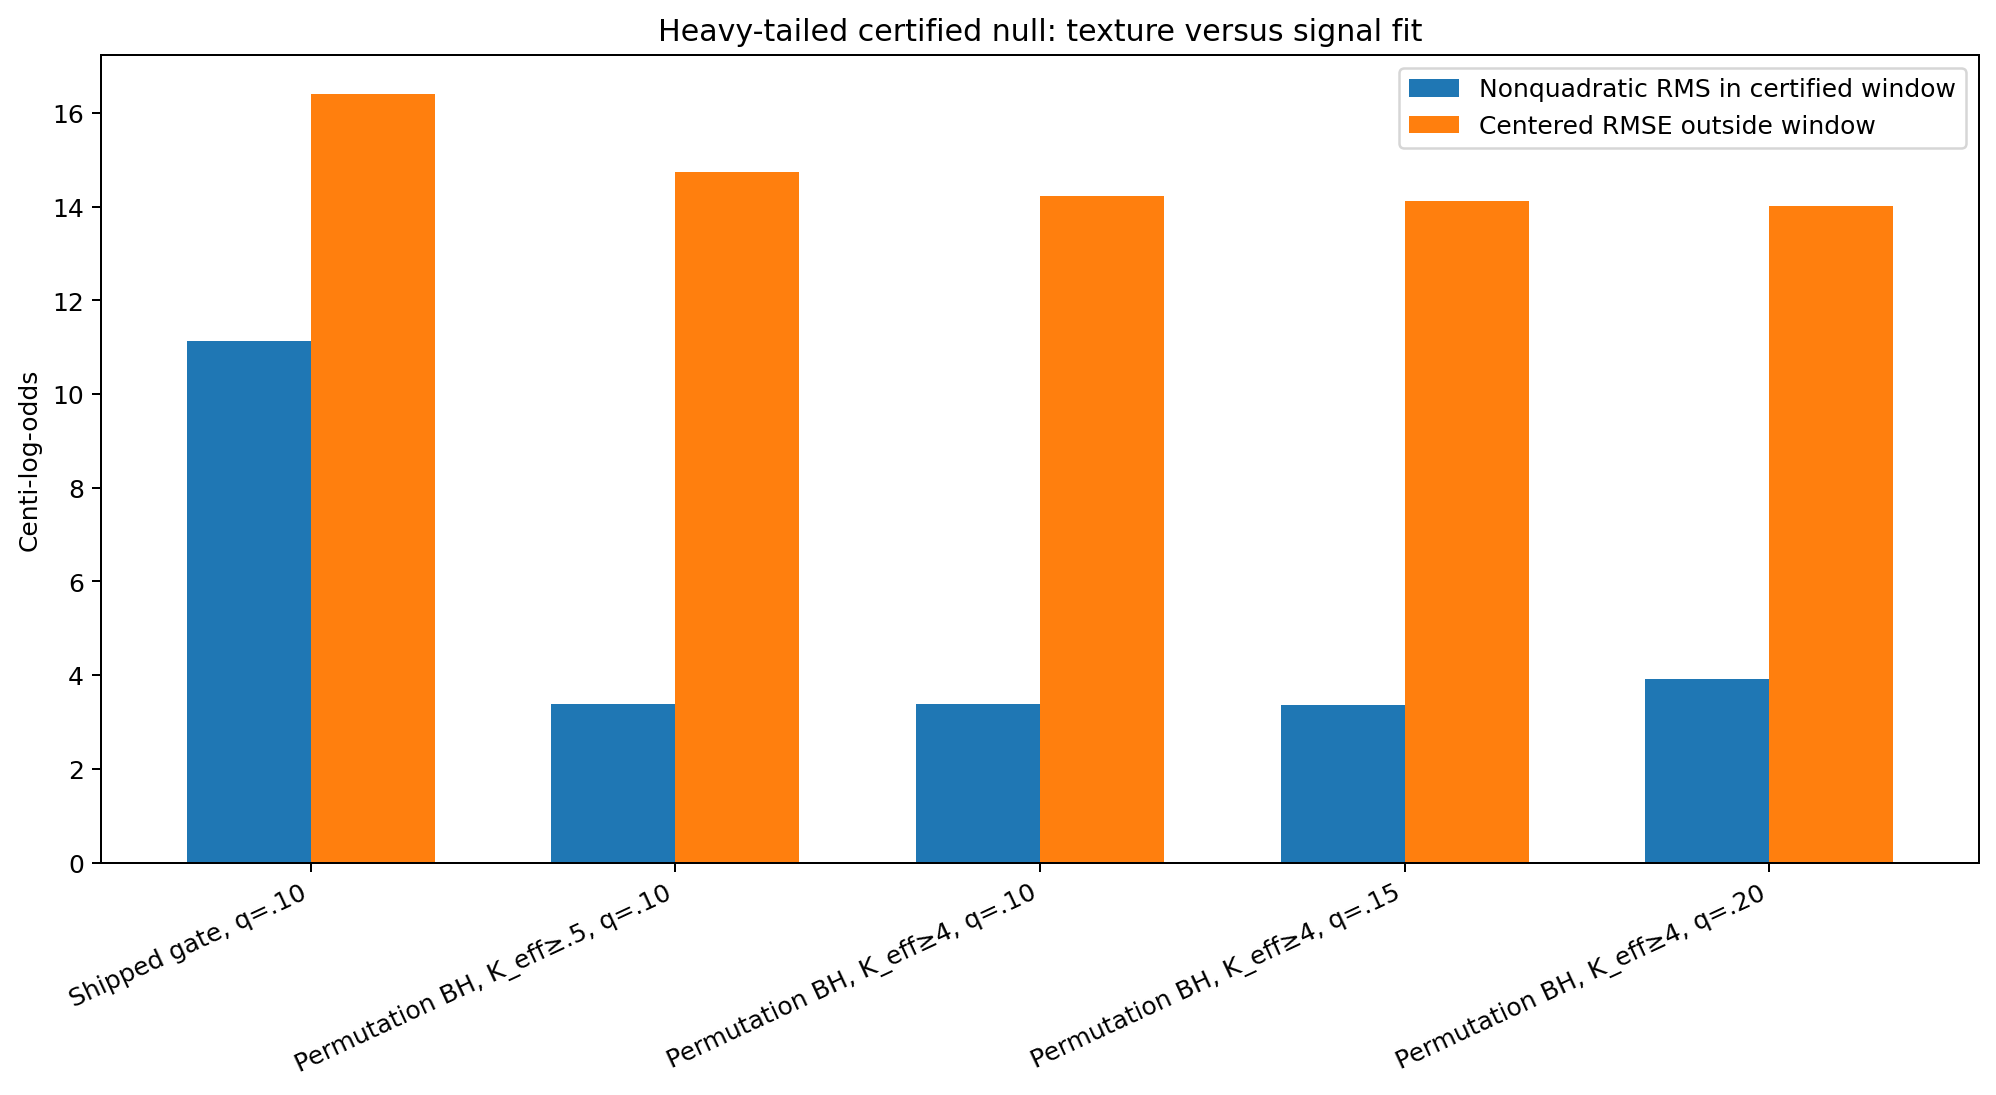
\includegraphics[width=0.92\linewidth]{heavytail_certified_fit_tradeoff.png}
\caption{Heavy-tailed certified-null tradeoff over twenty seeds. The pooled
permutation rules sharply reduce nonquadratic texture inside the certified
window while preserving or improving the low-order signal outside it.}
\label{fig:heavytail-certified-tradeoff}
\end{figure}

The real-data result prevents adoption. On the unfiltered April proxy,
$K_{\mathrm{eff}}\ge4$, $q=.15$ increased mean held-out deviance from 6.5830
to 7.1445 across ten matched splits. After the WALA-zero audit and full refit,
the gap narrowed but remained: 6.4968 versus 6.8108, worse in all ten splits
(Table~\ref{tab:no-wala0-real}). The pooled-permutation gate has therefore
solved the tested null-size problem more convincingly than the legacy gate,
but its hard support/depth bottleneck discards useful localized structure in
the real cross-section. The next experimental target is a depth-aware support
rule or a hybrid gate that preserves candidate-specific permutation
calibration without suppressing replicated descendants. The experimental
branch is not the released default.

\section{Measured noise physics and formation information}\label{sec:physics}

\textbf{Effective exposure has a ceiling.} A pool's information about the
surface saturates at $1/\sigma^2$: $n_{\mathrm{eff}} = n/(1+npq\sigma^2)$,
about $18$ loans at typical rates and $\sigma^2=0.35$. The April file's
$47.6$M loans are $4.2$M effective loans for surface estimation, and its
$32$ mega pools are ${\approx}18$ effective loans each. Fitting, testing,
or scoring at nominal $n$ where $n_{\mathrm{eff}}$ belongs is the single
mechanism behind the cluster pathology, the deviance tail, and the null
miscalibration.

\textbf{The mixing law is not Gaussian.} The per-size instrument
(face-level cross-pool moments remove local surface bias; falsified clean
on the null benchmark) reads $\sigma^2(n)$ near-flat at $0.26$--$0.47$.
The shape test against the fitted binomial-Gaussian mixture rejects:
standardized-residual tails run $12.5\times$ the mixture at $|r|>6$ and
$77\times$ at $|r|>10$ (excess kurtosis $67.7$ against $3.3$), while pools
with $n\ge10^4$ are lighter-tailed than modeled. The mixing law is
size-dependent in shape; the permutation null of
Section~\ref{sec:nulls} prices this without modeling it.

\textbf{Pool formation is an insider partition.} Within-cell constructed attrition proxy
rises $+0.11$ per e-fold of loan count and $+0.88$ per e-fold of average
loan size; the loan-size loading sign-flips with seasoning ($-0.21$ young,
$+0.79$ seasoned: credit-event and refinancing channels load on balance
with opposite signs). Issuer identity alone explains $18.9\%$ of residual
within-cell pool variance (issuer sd $0.30$ log-odds), and multi-issuer
pools, which have no single grouping agent, carry $5.4\times$ less
residual variance than single-issuer pools. Grouping metadata forecasts
the pool effect; in an overlay deployment the base model is assumed to own
borrower-side balance effects, and formation and servicer effects are the
overlay's cargo.

\section{The loan-level formulation}\label{sec:loanlevel}

Balance-dependent refinancing removes exchangeability of loans within a
pool: the future data model treats each loan as its own trial, sharing
only its pool's effect,
\[
Y_{Pj}\sim\mathrm{Bernoulli}\bigl(\operatorname{logistic}(\eta_0(b_{Pj},z_P)
+ g(z_P) + u_P)\bigr),
\]
with $b_{Pj}$ the known loan balance. Seven consequences, each validated
by simulation (\texttt{loanlevel\_sim\_issues.py}; $\beta=0.5$ per
log-balance, $\sigma^2=0.35$).

(1) The conditional law is Poisson-binomial and under-dispersed:
$\operatorname{Var}(k\mid u)=\sum p_jq_j$ (simulated $87.9$, formula
$88.0$) against the binomial $n\bar p\bar q = 91.7$; the binomial noise
floor is an over-estimate. (2) Aggregation does not commute with the
link: at fixed mean $\eta$ the expected rate falls with balance
dispersion ($0.646\to0.625$ across dispersion $0\to1.8$), and pool-level
regression on mean balance recovers $0.42$ for a true $0.5$. The
estimand must move to the loan level; pools are known weighted integrals
of it. (3) Information is concave: $\sum p_jq_j \le n\bar p\bar q$, so
nominal pool information overstates loan-sum information. (4) The pool
effect is a one-factor structure with loadings $p_jq_j$: near-saturated
loans barely reflect their pool's effect; pairwise covariances follow
$p_jq_j\,p_{j'}q_{j'}\sigma^2$; loading-correct moment estimation
recovers $\sigma^2 = 0.320$ where naive $npq$ weighting gives $0.264$
(truth $0.350$). (5) The residual moment bias is an expansion-point
artifact: anchoring the delta method at each pool's posterior mode
$\hat u_P$ rather than the prior shrinks the error base $22\times$
(posterior variance $0.016$ against $\sigma^2=0.35$) and the
fixed-point estimator recovers $0.347$. The same-data ladder closes the
question of higher orders: mode Laplace $0.36407$, fully exponential
second order $0.36488$, exact mode-centered quadrature $0.36489$; the
correction closes the deterministic gap to $5\times10^{-6}$ while the
exact estimate sits $0.7$ sampling deviations from truth. The
approximation is not the binding error. Production recipe: Laplace above
a curvature threshold, mode-centered GH below, second order as
cross-check.

(6) Identification is the headline. Within-pool balance contrasts
difference out $u_P$: the fixed-effects fit recovers
$\hat\beta = 0.497$ even under informative formation
($\operatorname{corr}(u,\text{balance})=0.6$), where pooled estimation
reads $0.651$: a $30\%$ upward bias, pool effects laundered into the
balance curve. For specified pools, balance-homogeneous by construction
(within-pool sd $0.05$), the FE standard error explodes $18\times$ and
pooled reads $0.812$: the confounding concentrates exactly where
formation is most informative, so balance coefficients in spec-pool
strata are identified only across pools and must be flagged as
model-dependent. (7) Estimation: the pool-level Laplace mixed likelihood
(one 1D log-concave integral per pool, $u$ integrated against the
Bernoulli product) jointly recovers $(\hat\beta, \hat\sigma^2, \hat a_0)
= (0.503, 0.365, 0.604)$ on $120$k loans in $1{,}500$ pools; this is the
estimation engine for the loan-level mesh, with issues (1), (3), and (4)
priced automatically. The permutation null generalizes by permuting
pools carrying their loan bundles intact, conditioning on realized
compositions.

The architectural consequences: the mesh, gate, and lfdr machinery are
unchanged; the working linearization per loan sits at
$\eta_0 + g + \hat u_P$ (posterior anchoring as the linearization
discipline); $K_{\mathrm{eff}}$ counts pools of loans; and within-pool
balance variation finally splits the single-snapshot bundle, since pool
idiosyncrasy is constant across a pool's loans while sub-face surface
varies with their coordinates.


\section{Tail shape: the kurtosis program}\label{sec:kurtosis}

Status: all items measured on controlled benchmarks unless labeled
otherwise. The pool-effect law's shape, not just its variance, is a
load-bearing input. The measured excess kurtosis of standardized real
residuals is $67.7$ pooled across sizes (within-stratum recalibration
below: the pooled figure mixes scales); a Gaussian-mixed binomial compound produces
essentially zero at any $\sigma$ (measured: $-0.05$ across
$\sigma^2 = 0.12$ to $2.0$), so the kurtosis is a direct measurement of
the non-normality of $u$. The controlled instrument is a
variance-preserving lump mixture: with probability $\pi(n)$ the pool
effect is scaled by $L$, normalized so $\mathrm{Var}(u)$ is unchanged;
$(\pi, L) = (0.035, 17)$ reproduces the real kurtosis. At that setting
$91\%$ of the effect variance is carried by $3.5\%$ of pools.

\textbf{Translation to the null.} For a candidate with effective
replication $K_{\mathrm{eff}}$, the null statistic's excess kurtosis is
$\kappa_4(u)/K_{\mathrm{eff}}$ (simulation matches across two decades).
Deep candidates on the real design run at median $K_{\mathrm{eff}}
\approx 2$ to $3$ (measured via a score diagnostic), so effect kurtosis
arrives at deep admission decisions nearly undiluted:
Gaussian-equivalent three-sigma cuts are $z \approx 7.5 / 6.2 / 5.1$ at
$K_{\mathrm{eff}} = 2/4/8$. A pipeline experiment with the effect
kurtosis dialed to $\{0, 10, 33, 69\}$ confirms the in-window null
score kurtosis climbs accordingly (e.g.\ depth-6: $6.7 \to 26.9$),
with the caveat that candidate populations under default dynamics are
selection-conditioned; a forced-uniform-refinement rerun is queued to
isolate the marginal law.

\textbf{What kurtosis does not damage.} On a clean benchmark (cosine
product signal, uniform locations, $500$k pools, kurtosis dialed at
fixed variance) the surface fit is unaffected to slightly improved:
rms error $13.99 \to 12.30$ centi-logits from kurtosis $0$ to $69$, and
held-out deviance in excess of the oracle is constant at $0.54$ to
$0.58$. Lumpy noise concentrates the same variance in fewer pools; the
information-weighted average is dominated by the quieter majority
wherever replication is high. Damage is confined to low-$K_{\mathrm{eff}}$
decisions, certification counts, and per-pool posterior tails.

\textbf{The posterior transform.} Posterior effect estimates carry
kurtosis $\lambda^2 \kappa_u$ with $\lambda = \sigma^2/(\sigma^2 + v)$
the pool's reliability; exact at moderate kurtosis, attenuated at the
extreme by outcome saturation. The law inverts to a measurement tool:
divide observed posterior kurtosis by $\lambda^2$ per size class.

\textbf{Estimator diagnosis.} At kurtosis
$69$, truth $\sigma^2 = 0.35$: robust scale reads $0.065$ (the quiet
core), Gaussian ML $0.108$ (a misspecified-model compromise), the
moment estimator $0.292$ (unbiased in principle; the deficit is outcome
saturation). Counts are bounded, so $k = n$ censors lump magnitudes;
the lump law stays identified through saturation frequencies, which is
what the repair uses. Details and the refuted intermediate hypotheses
are in the lab notes.

\textbf{The repair, validated.} An EM fixed point with the lump-mixture
prior and exact binomial likelihood (mode-centered Gauss-Hermite,
deterministic, no sampling, no logits) recovers all parameters at every
kurtosis level: at $69$, $\hat\pi = 0.0353$ (truth $0.035$),
$\hat\sigma_L^2 = 8.96$ (truth $9.13$), total variance $0.361$ (truth
$0.35$), implied kurtosis $62$; at kurtosis $0$ it degenerates
gracefully (near-equal components, implied kurtosis $0.1$, no phantom
tails). Residual $+4\%$ variance bias is surface-error leakage,
quantitatively matched to the measured fit rms. One estimation pass
supplies the total $\sigma^2$ for shrinkage, $(\pi, L)$ for the
four-moment or saddlepoint gate, and tail-aware posteriors that shrink
identified lumps less (mixture-posterior kurtosis $58$ versus $21$
under the Gaussian prior; correlation with truth $0.94$). Proposed and
queued: wire these into the admission gate; acceptance test is the
full-strength tail benchmark with pass criterion $53 \to$ single
digits.


\textbf{Real-data measurement.} Running the
mixture fixed point on the April 2026 file per size stratum: totals
$0.851 / 0.514 / 0.494 / 0.391$ for $n$ in $25$--$128$ / $128$--$512$ /
$512$--$4096$ / $4096{+}$, with wide-component weights $0.11$ to $0.27$
and scale ratios $5$--$6\times$: a broad two-population structure
rather than rare monsters. Within-stratum residual excess kurtosis is
$1.8 / 1.9 / 2.8 / 20.1$ with $P(|t|>4)$ of $12/20/27/194\times$
Gaussian: the pooled kurtosis $67.7$ was substantially a cross-size
scale-mixture artifact, and the heavy-tail problem concentrates at mega
pools, which are also the $K_{\mathrm{eff}}$-collapsing,
metric-dominating objects. Identified lump pools are one-sided with
opposite signs by size: small-pool lumps $86\%$ slow (mean $-1.35$
logits; an $n_0$-rounding data-artifact channel is queued for checking
before these are treated as physical), mega-pool lumps $73\%$ fast
(buyout-like). Consequences, proposed: per-stratum gate variances from
the fixed-point table (the hand-set $0.35$ underprices small-$n$
strata); tail-aware nulls needed most at mega-star candidates; the
full-strength adversarial benchmark retained as stress test but a
realistic-tails acceptance benchmark (mild small-pool tails, heavy
one-sided mega tails) replaces it as the pass criterion.


\section{One law in production and the corrected ledger}\label{sec:onelaw}

The admission null consumes the measured mixture directly. Per-stratum
pool variance enters the null variance as
$\sum_i w_i^2\phi_i^2\sigma_i^2/X^2$; the dispersion estimate deflates
each Pearson term by its own stratum's law; and tail thickness enters
through the candidate's fourth cumulant
$\lambda_4 = \sum_i a_i^4\kappa_{4,i}\sigma_i^4/\mathrm{Var}^2$, mapped
to a Gaussian-equivalent score by a strictly monotone probability match:
the null is modeled as a two-component Gaussian scale mixture with the
candidate's variance and $\lambda_4$, and the observed $z$ is carried
through its tail and an upper-tail probit. Where $K_{\mathrm{eff}}$ is
large the corrections vanish automatically; where a lump-capable pool
dominates, the deep threshold rises exactly there. A permanent
equivalence guard (one-law with a flat table reproduces the flat-gate
run exactly) protects the machinery, and the standard falsification
suite passes: the kurtosis-dialed cosine benchmarks at baseline power,
the certified counts below. Two implementation errors found and fixed
en route (a non-monotone quantile expansion; a dispersion normalizer
that halved $\hat\phi$ under the held-out split) are documented in the
lab notes; the second affected all earlier split-run numbers, so the
ledger is re-baselined here.

Currency check (this revision). All ledger pins were re-verified on the
current binary, which carries every flag-gated mechanism of
Section~\ref{sec:boundary} in its default-off state: composite
$q{=}0.30$ held-out deviance 10.488 (bit-exact, with the recorded
\texttt{DMESH\_GATE\_EXTRA\_VAR=0.35}); one-law 1527 vertices / 9.399
and one-law with law weights 2021 / 10.261 (both bit-exact); certified
counts v3${}=2$, v4${}=7$ re-run \emph{with the quadratic prior
enabled}, i.e.\ under the production configuration, unchanged. Two
caveats now on record. First, guard values are pinned per build: the
flag-off deviance of the quadratic-prior configuration showed
$\pm 0.1\%$ sensitivity to floating-point contraction across rebuilds
(10.798--10.808); vertex counts were stable throughout, so counts are
the cross-build invariant and deviances are the per-build one. Second,
the offset was certified \emph{end to end}: the production offset
recipe (plain two-exponential age ramp, coefficients fitted on the
train half) was estimated on each null dataset exactly as it would be
in production, and the full pipeline run on the result. Certified
counts: v3${}=2$ (unchanged), v4${}=3$ (quieter than the zero-offset
7): the offset absorbs level that the mesh otherwise builds, and the
gate stays honest on what remains. The audit also caught a defect
worth recording: a WAC-interaction variant of the offset, unregularized,
reached $\pm14$ logits at sparse band corners of the null datasets. It
was already dominated on real data by the plain recipe (held-out NLL
2.9365 vs 2.9408) and is excluded from production; offset designs with
interactions require regularization before use.

Ledger, post-fix. Certified-false deep faces: composite gate $2$ (v3)
and $7$ (v4), unchanged. Default gate $969$ (v3) and $996$ (v4)
on current code. Real April 2026 at $q=0.30$: composite $1857$
vertices, held-out deviance $10.488$; one-law $1527$ vertices,
$9.399$: honest pricing gives the smaller mesh and the better held-out
fit. Under the corrected law the $q$ dial recalibrates
($q=0.10$ now sits where roughly $q=0.02$ sat) and the held-out
deviance spread across the dial collapses.

Residual micro-structure the mesh cannot represent (measured; remedy
queued): a $48$ centi-logit sawtooth in residuals by WAC position
within the $0.5\%$ coupon grid, discontinuous at the Ginnie II
assignment boundary (servicing-spread position within coupon), plus a
$12$ centi-logit annual origination-seasonality cycle. Both are
covariates, not surface: coupon re-parsed from the file, spread and
seasonality into the observation offset, then the mixture law
re-estimated, since part of the fitted pool variance is this structure
in costume.


\subsection*{The completed system: joint fixed point and stratum means}

Status: measured, end of session, \emph{April-proxy era} (NLL scale
$\sim$2.98). Section~\ref{sec:aug5} rederives this fixed point on the June
SMM design under the exact solver and retracts the SMM-era law estimated
inside the oscillating external experiment; the design principles below
stand. The law now feeds all four consumers:
the gate (per-stratum variance and tails), the IRLS working weights
(per point, including stage zero, which retires binomial-weight mega
domination at its source), the per-pool posteriors (mixture
responsibilities and effects), and the held-out metric, evaluated by
reference with the same law object rather than a refit. Surface and law
are alternated to mutual consistency with damped updates; the law
converges in about two iterations to a few-percent band, and the
residual run-to-run wobble at fixed law ($\pm10\%$ in mesh size)
lower-bounds any fixed point's tightness and is the multi-seed pass's
measured target. One instability found and designed around, one
sentence's worth: per-pool responsibility-weighted \emph{working}
weights are self-exciting (down-weight, surface departs, lumpier,
down-weight) and oscillate; weights therefore consume the stratum law,
per-pool variances are reserved for the gate. Law-priced weights
deliver held-out mixture NLL $2.977$ to $2.994$, at that point the best
predictive scores in the program, from the certification-grade gate.

A held-out Q-Q verification of the law (probit of the predictive PIT
per stratum) shows the two-component mixture near-exact through two
sigma and cutting the three-sigma tail excess roughly threefold versus
a variance-matched Gaussian, with a quantified residual ($1.3$ to
$1.9\times$) in the populated strata.

The residual histograms then exposed differing \emph{means} across size
strata, and extending the law with a per-stratum mean $\mu$ measures
the formation size gradient directly: $\mu = -0.34 / -0.02 / +0.25 /
+0.11$ across the four strata, matching the count effect in magnitude.
Consequences: the small-stratum law deflates (total $0.71\to0.60$,
lump weight $0.27\to0.21$; the $512$--$4096$ lump weight halves), the
small-pool lump one-sidedness largely dissolves (approximately
symmetric about the stratum mean; the mega fast-skew survives), and
held-out mixture NLL improves $3.000\to2.945$, the largest single
metric gain in the program, from four numbers. The mega $\mu$ is unstable across the
even/odd split (a handful of giant pools dominates either half) and
wants shrinkage or cross-vintage estimation. Design conclusion: $\mu$
is signal, not noise; it belongs in a per-observation offset, one hook
serving the three measured covariates the smooth surface cannot
represent (size gradient, coupon-spread sawtooth, origination
seasonality), after which the law is re-estimated on corrected
residuals.

Working set: default gate (predictive bound), composite $q=0.10$
(certification) and $q=0.30$ (production), the one-law gate as
successor under validation, the pooled-permutation gate implemented in an experimental branch with exact moments and deterministic pooled draws, but parked from production because of the real-data power loss; mixture-EM parameter report, held-out mixture NLL
(headline), deviance (secondary), certified-false counts, the confound
and chirp falsifiers, and the PIT audit. Retired branches live in the
lab notes, not here.

\section{Dynamics on frozen nodes (summary)}\label{sec:dynamics}

For completeness: after the static fit, freeze the geometry and refit heights monthly
by the exact WLS normal equations (iterative sweeps leave smooth-mode residue an order
of magnitude above the theoretical noise; the monthly system is small, solve it), with
per-month reinitialization so measurement errors are independent across months. The
population kinematics are known (aging $\dot a=1$, common incentive drift), so the
transport term of the McKendrick--von Foerster description is imposed, not estimated:
build the panel in the Eulerian frame (fixed $(a,c)$ cells, jointly binned so
composition drift does not masquerade as decay) and the Lagrangian frame (fixed vintage
labels); the attached frame is the one in which the panel is separable
(cell profile $\times$ common decay $=$ rank-1 up to noise), and the decay $\lambda$ is
read off by an errors-in-variables-robust AR regression with lagged instruments in the
winning frame. This is the frame-aware upgrade of the fixed-partition autocorrelation
study: persistence quantifies signal decay (hence horizon and turnover), and the frame
answers whether the mispricing travels with the collateral or with the region of state
space.

\section{Legacy boundary investigation and the limits of working-scale adaptivity}\label{sec:boundary}

This section preserves a historical solver-forensics program on an older
Ginnie snapshot whose raw input is no longer available. It was useful for
identifying failures of local working-scale scoring, but it is not a
reproducible claim about April 2026 SMM. The current single-snapshot April
response is the constructed attrition proxy defined in
Section~\ref{sec:realdata}, and its WALA-zero boundary is measurement
contaminated as shown in Section~\ref{sec:wala0-audit}. The numerical claims
below should therefore be read as legacy stress tests of the optimization and
refinement machinery, not as substantive mortgage-performance estimates.

\subsection{Historical boundary phenomenon and corrected plotting rule}

In the unavailable historical snapshot, the WAC 5.75--6.25 band had a pooled
WALA 0--2 binomial rate corresponding to $-7.49$ log-odds. Every mesh
configuration fitted the base of that cliff between $-2.5$ and $-3.5$, an
error of about four logits confined to the first eight coordinate months.

The plotting correction remains valid independently of the snapshot:
band-averaged empirical logits with the $+\tfrac12$ correction floor each
$k=0$ pool at $-\log(2n)$. In the historical edge slice, 97\% of pools had
$k=0$, so averaged empirical-logit dots read $-4.49$ where the pooled rate was
$-7.49$. Fitted surfaces that dove past $-4.5$ therefore appeared to overshoot
while improving exact binomial NLL. At saturated edges, profile dots must use
the pooled rate $\sum k/\sum n$, never an average of corrected empirical
logits. This statement concerns display and likelihood arithmetic; it does not
rescue the April WALA-zero proxy as SMM.

\subsection{Two working fixes and a benchmark}

Two additions materially improved the edge. First, a locally quadratic
shrink target (Dubuc--Deslauriers along the parent edge, one-sided at
boundaries) moved the base from $-2.54$ to $-3.45$ and improved
held-out mixture NLL from 3.0000 to 2.9838 with certification
unchanged. Second, a per-pool offset column carrying a two-exponential
age ramp fitted on the training half moved the base to $-6.57$ and the
NLL to 2.9365, the best mesh result in the program; the ramp-region
NLL (2.211) essentially matches a law-weighted tensor-spline GAM
benchmark (2.159), which reaches $-8.05$ at the base by running full
IRLS on a fixed basis with an effectively unpenalized fit. The GAM
wins overall NLL (2.9045) by a thin margin distributed over the
mid-band, where it also produces 11.0 centi-logits rms of spurious
structure inside the certified window against the mesh's 4.4: the
familiar trade, prediction against policed attribution.

\begin{figure}[t]
\centering
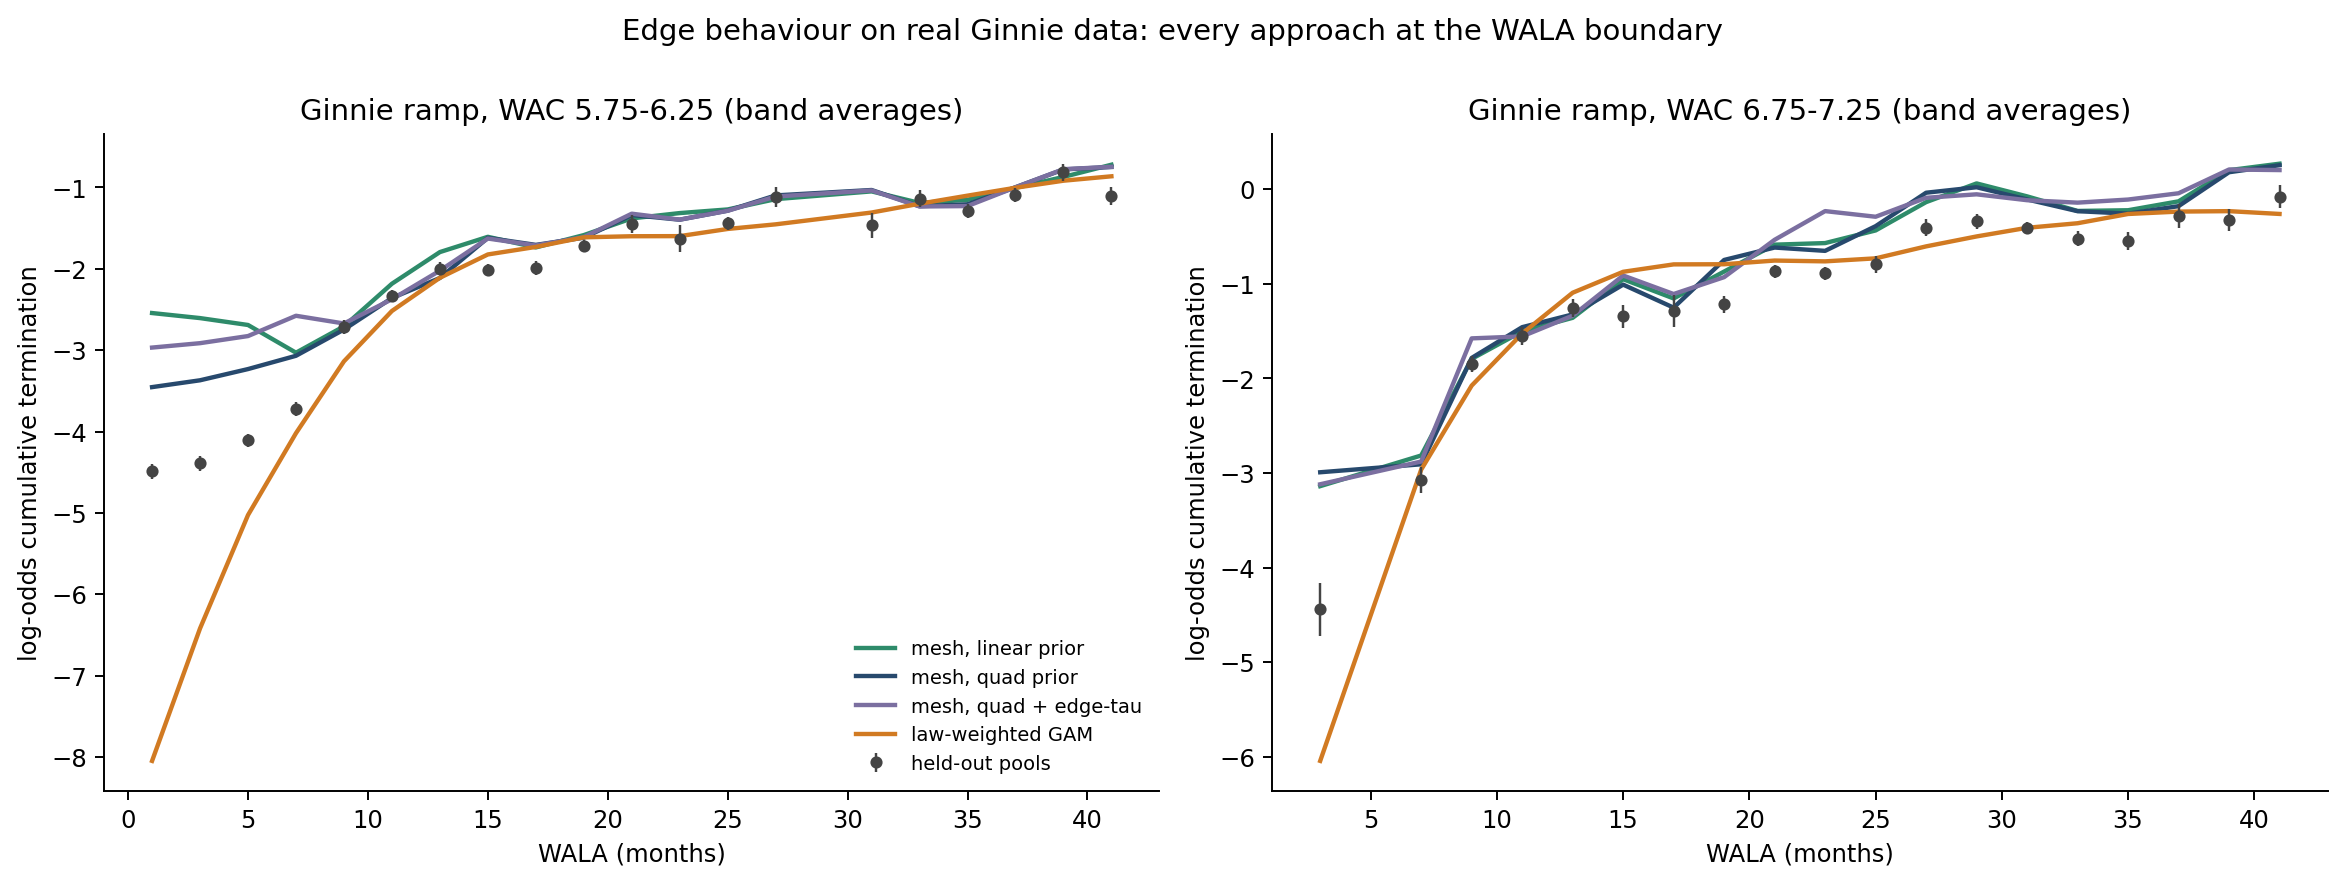
\includegraphics[width=\textwidth]{ginnie_edge_approaches.png}
\caption{Every approach at the real WALA boundary, band-averaged
against held-out pools. All methods miss the base and bracket it from
opposite sides; differences vanish by WALA 10--12. (Dots here are
empirical-logit band averages; per the amended standard, the floored
region WALA $<8$ is re-measured with pooled-rate dots in the text.)}
\label{fig:edgeapproaches}
\end{figure}

\begin{figure}[t]
\centering
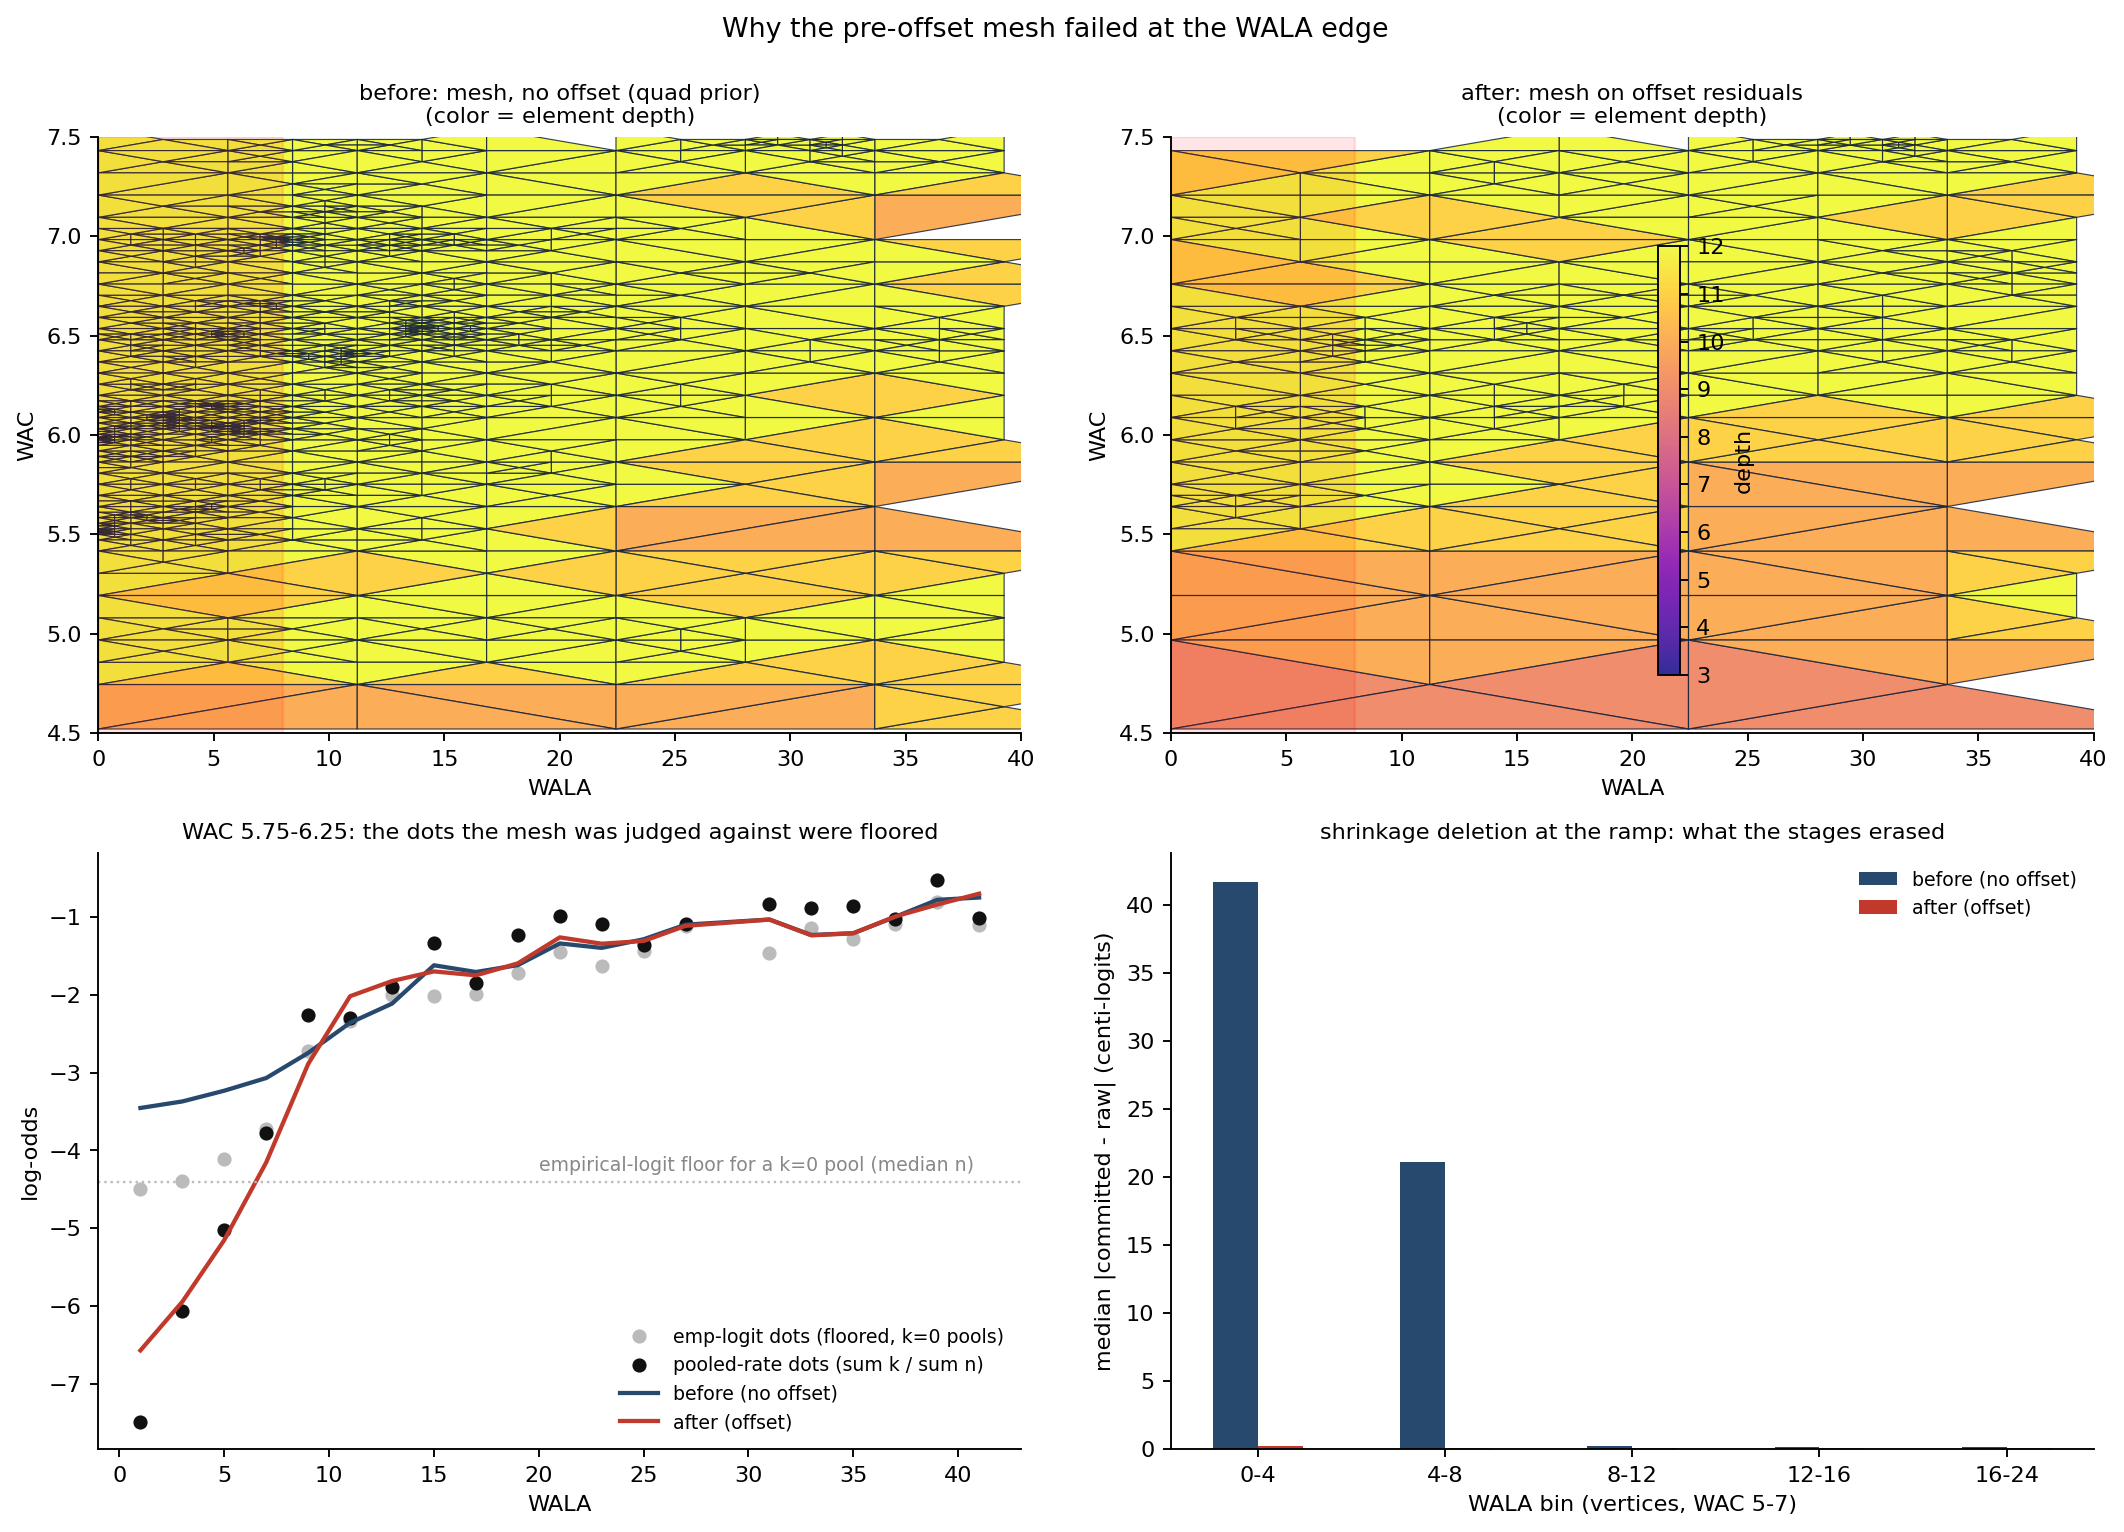
\includegraphics[width=\textwidth]{edge_failure_explained.png}
\caption{Why the pre-offset mesh failed. Top: mesh in the ramp region
before and after the offset (1{,}862 elements at median depth 17 in
the WALA $<8$ strip versus 507 at depth 14): detection was never the
problem. Bottom left: empirical-logit dots sit on the $k=0$ floor
line; pooled-rate dots reveal the true $-7.49$ base. Bottom right:
staged shrinkage deleted 42/21 centi-logits per vertex at the ramp
before the offset, 0.2 after.}
\label{fig:edgefailure}
\end{figure}

\begin{figure}[t]
\centering
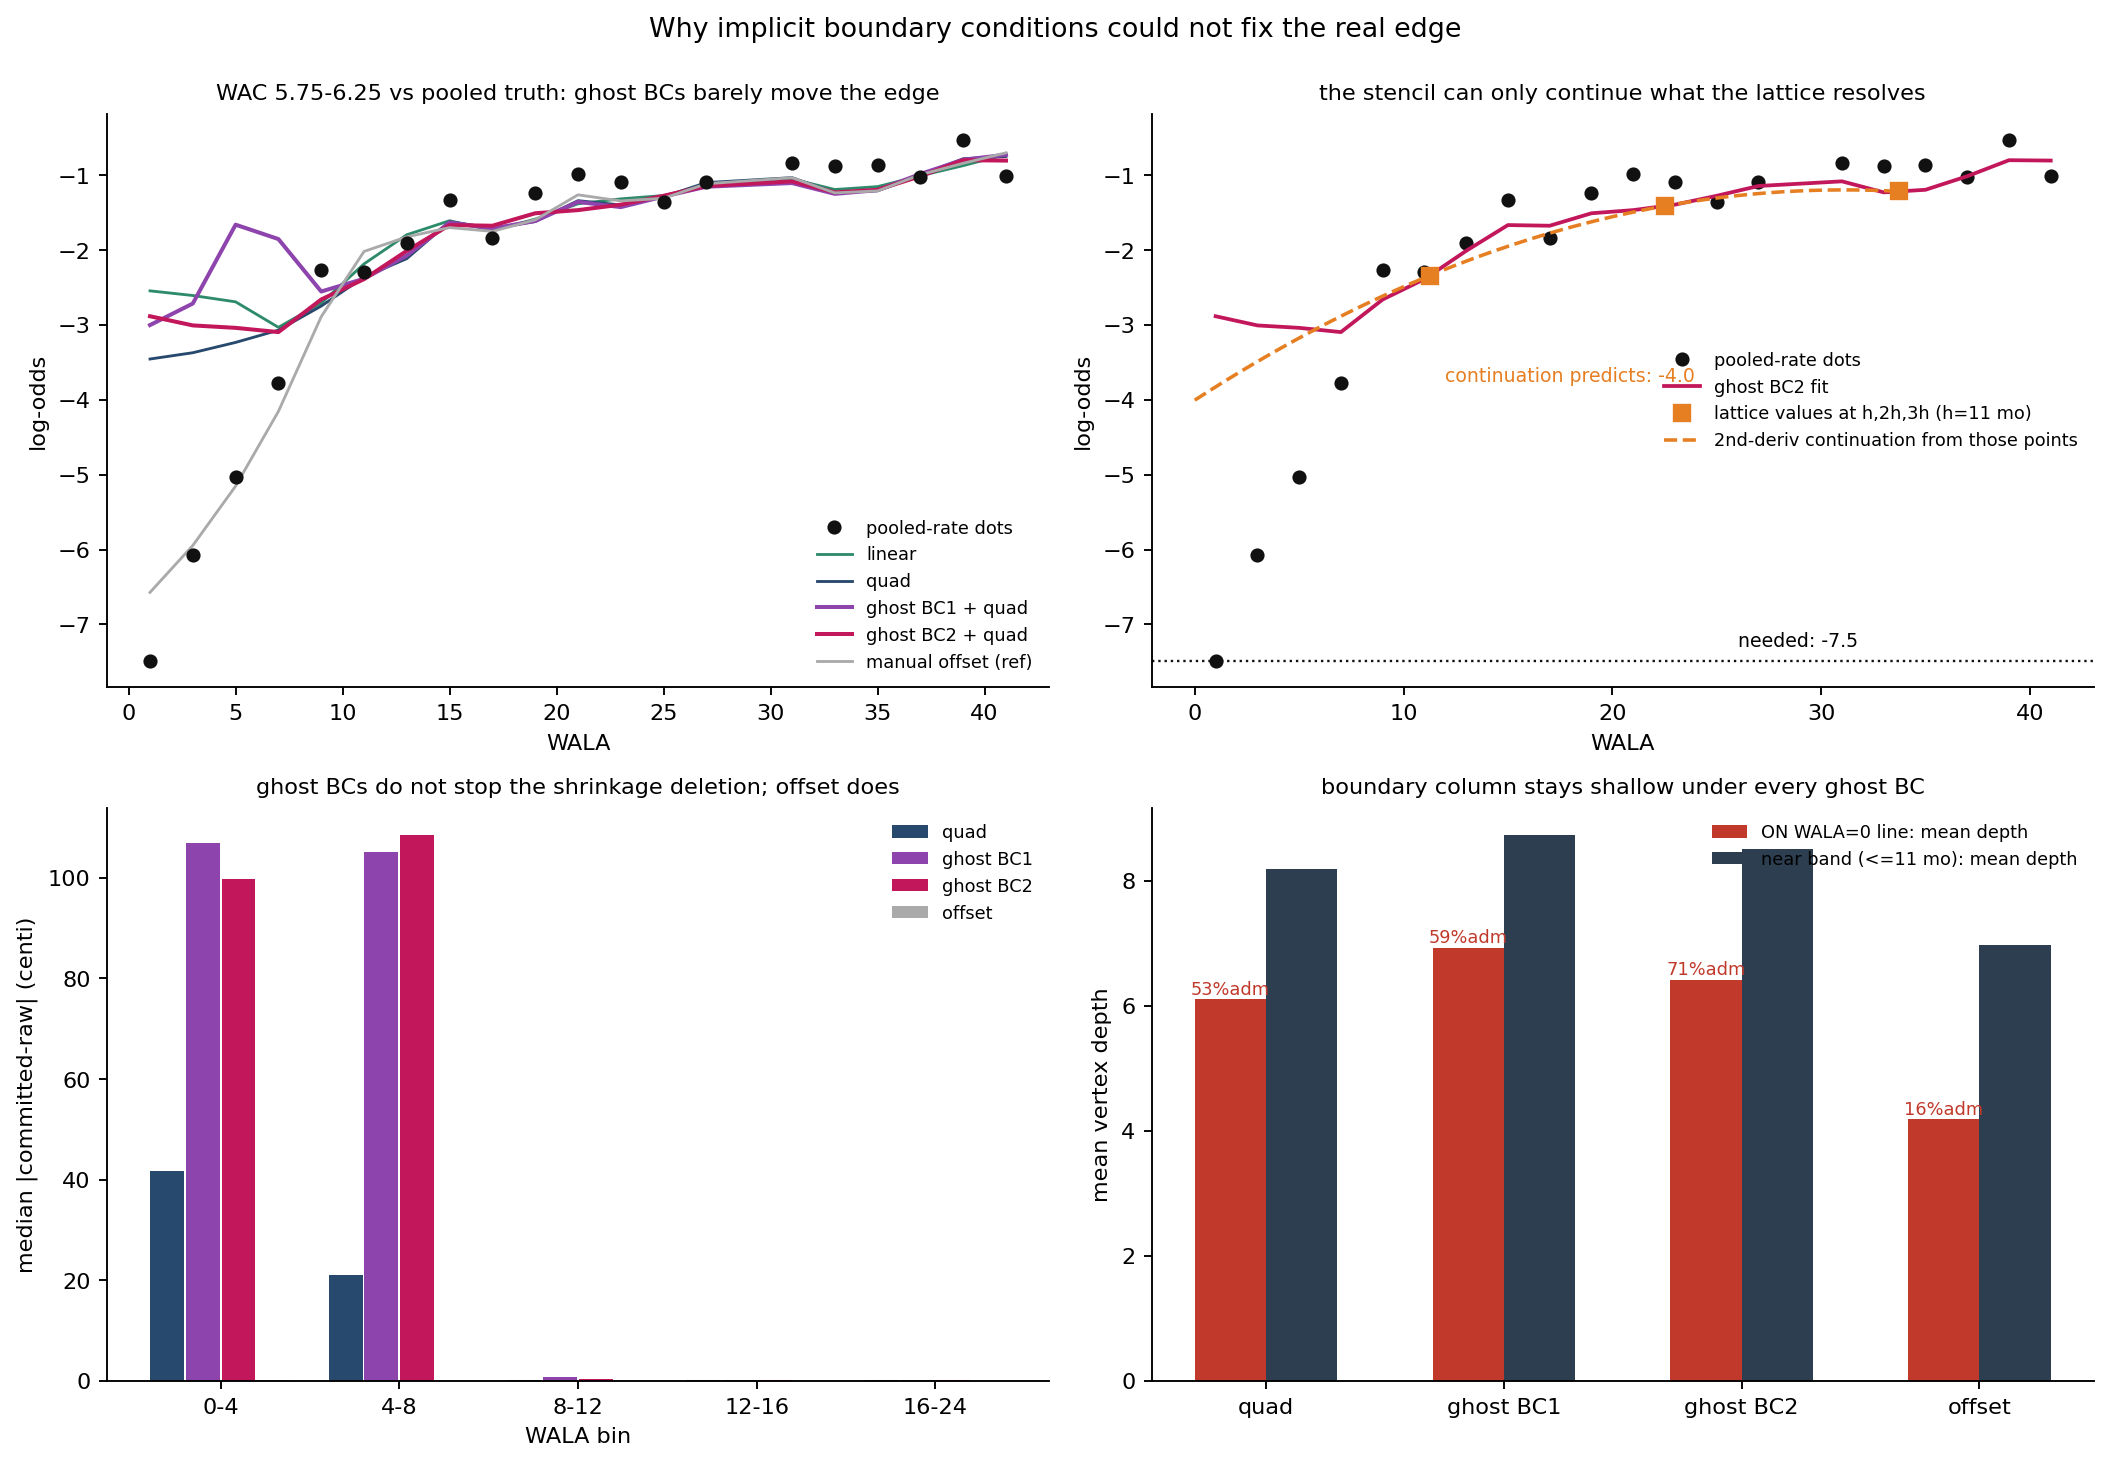
\includegraphics[width=\textwidth]{ghost_bc_explained.png}
\caption{Implicit boundary conditions priced. The second-derivative
continuation from the lattice values the boundary stencil can reach
predicts $-4.0$ where $-7.5$ is needed: a resolution ceiling, not a
stencil-order problem. Ghost BCs doubled the shrinkage deletion while
improving admission, and the surface did not move.}
\label{fig:ghostbc}
\end{figure}

\begin{figure}[t]
\centering
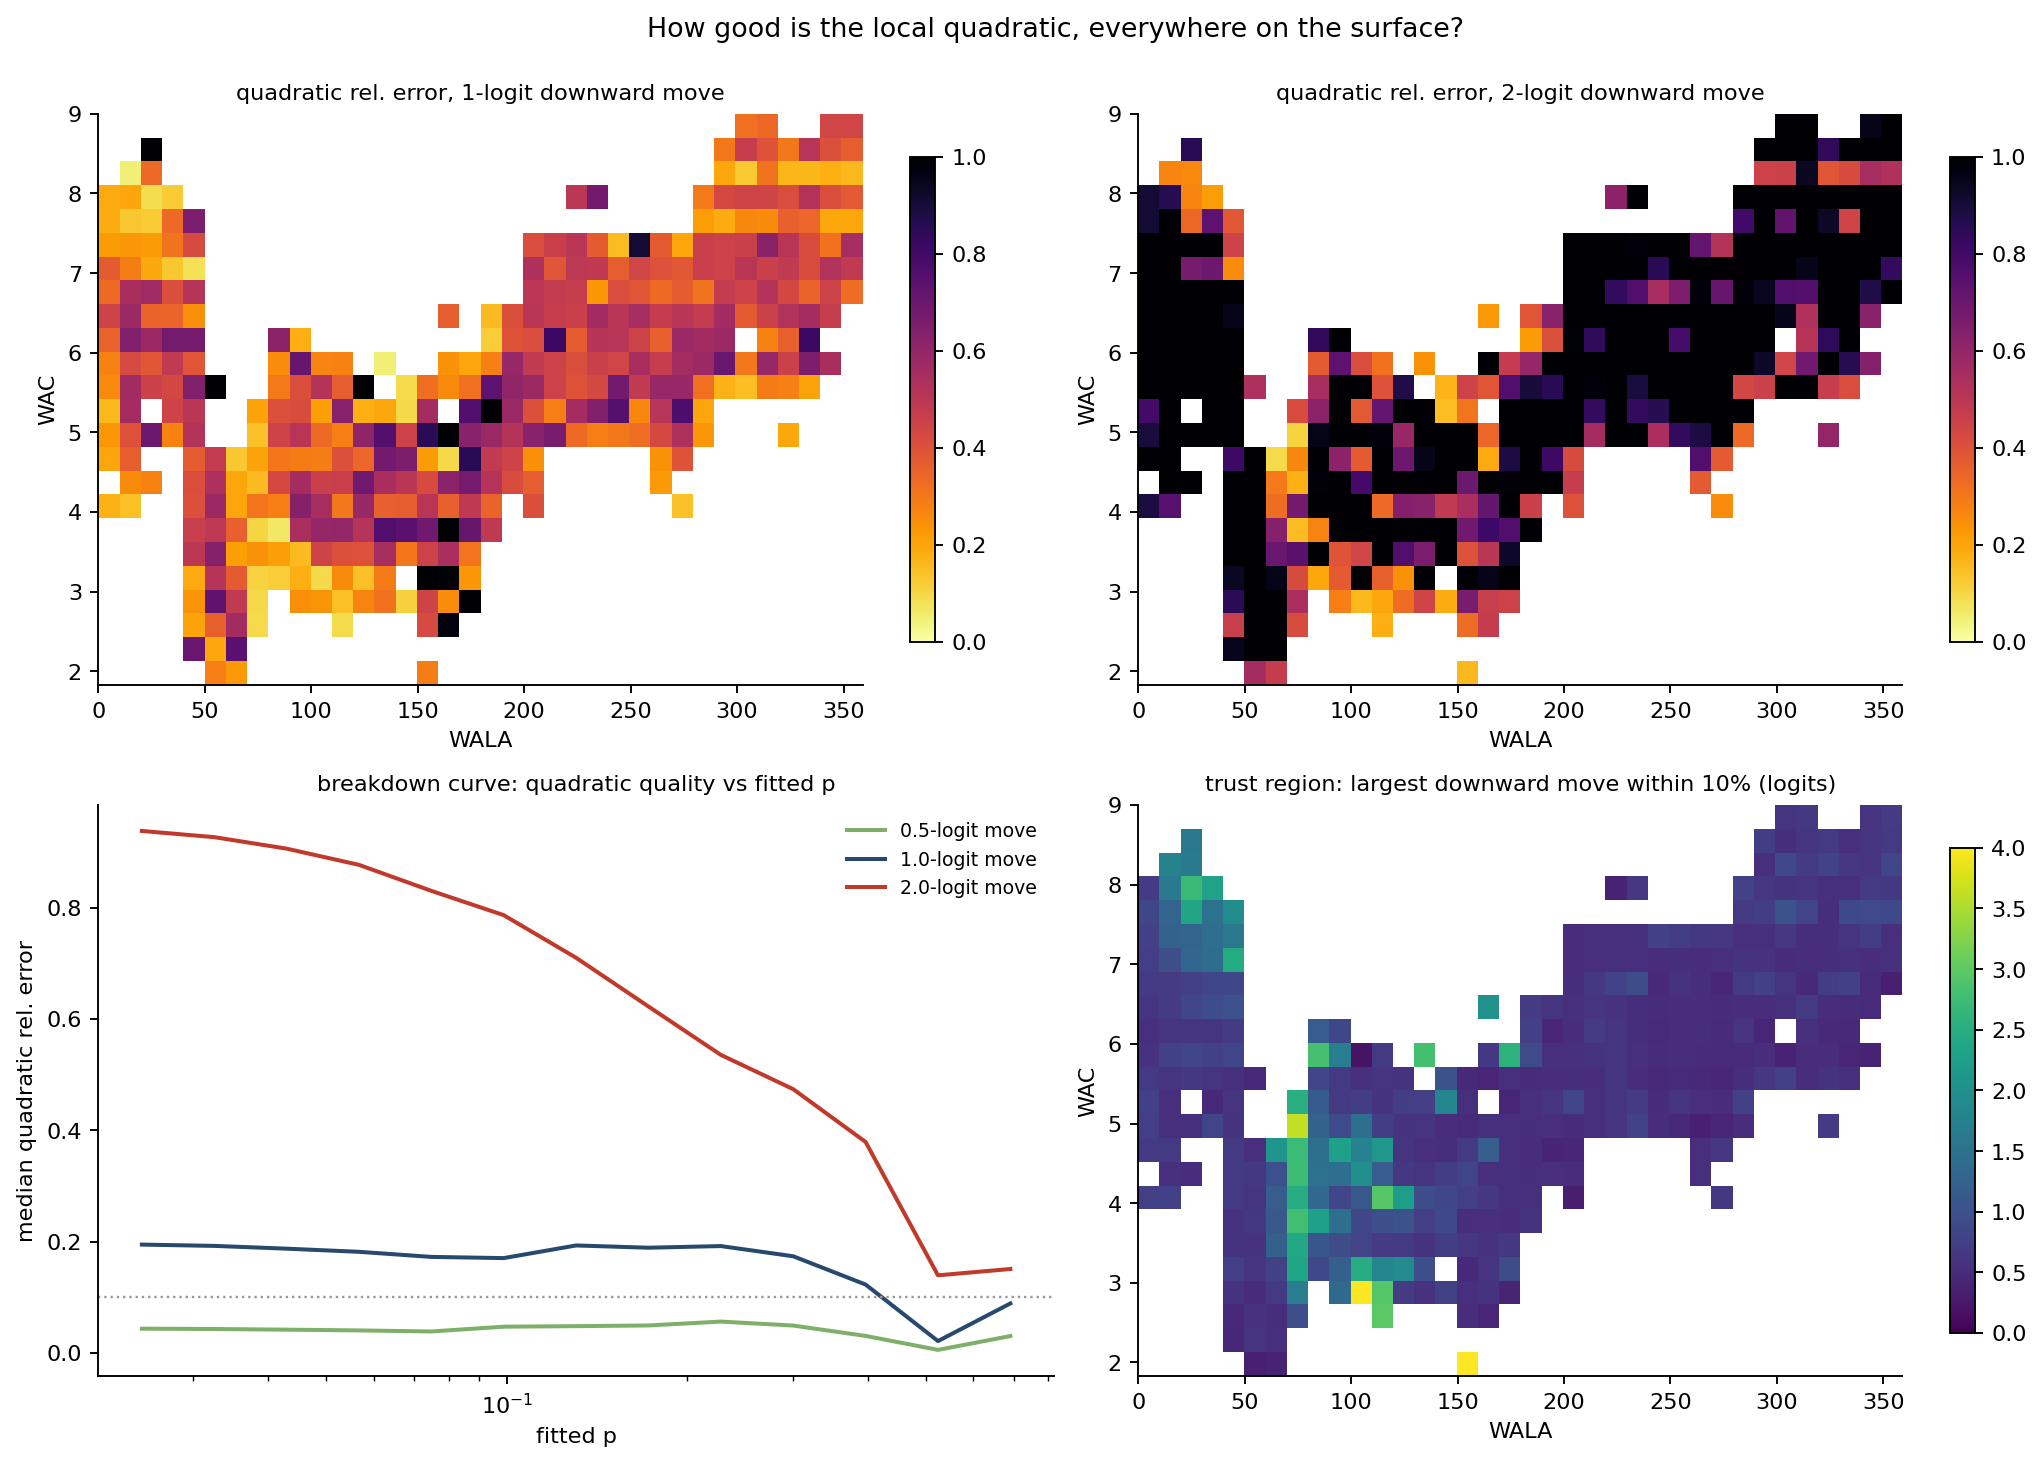
\includegraphics[width=\textwidth]{quadratic_quality_map.png}
\caption{Quadratic quality everywhere. The 10\% trust region is
0.5--0.75 logits across the whole surface; the edge is distinguished
by the size of the required move (4.5 logits), not by uniquely bad
quadratics at one-logit scale.}
\label{fig:quadquality}
\end{figure}

\subsection{The forensic ledger}

Ten mechanisms were priced against the edge. Each is flag-gated in the
tree, each reproduces bit-stable baselines when off, and each verdict
below is measured, not argued.

\begin{center}
\begin{tabular}{p{4.6cm}p{3.1cm}p{5.6cm}}
\toprule
mechanism & edge result & verdict \\
\midrule
linear prior (baseline) & base $-2.54$ & under-dives \\
quadratic prior & base $-3.45$ & adopted; insufficient alone \\
log-WALA coordinates & worse everywhere & rejected \\
prerefine 48/96 & ramp worse & wrong layer \\
boundary $\tau$ scaling & synthetic yes, real no & real edge evidence biased at $p\to0$ \\
ghost BC, 1st/2nd derivative & real base $-2.9$ & continuation capped by interior resolution ($-4.0$ ceiling, measured) \\
untaxed converged sweeps & base $-2.80$ & proposals themselves stall at $-4.03$ \\
admit-all (gate open) & base $-2.93$ & allocator, not the test, starves the edge \\
honest decision scores only & base $-3.05$ & allocation moves, commits do not \\
manual age-ramp offset & base $-6.57$ & works; per-dataset crutch \\
\bottomrule
\end{tabular}
\end{center}

\subsection{Why: the trust region and the misallocated information}

The edge strip (WALA $<8$, WAC 5--7) contains \emph{more} total Fisher
information than a same-width mid-band strip (6{,}425 vs 3{,}769 units
of $\sum n_i p_i(1-p_i)$); the band-mean logit is pinned to
$\pm 0.0125$. The data is sufficient. What fails is the currency in
which every internal decision is denominated. Measured across all
120{,}595 pools at the production fit: the local quadratic model of
the pool log-likelihood has a 10\%-accuracy trust region of 0.5--0.75
logits essentially everywhere on the surface; 43\% of pools exceed
20\% error already at a one-logit move; only 4\% of pools have a
four-logit trust region. Mid-band this is harmless because converged
fits make candidate moves centi-logit sized. At the edge the required
move is 4.5 logits, nine trust radii. One $k=0$ pool with $n=150$
gains 7.6 nats moving from $-2.95$ to $-7.5$; its working-scale score
for the same move is a fraction of a nat. Refinement ranking
($\hat\delta^2 x^Tx$), gate admission, and EB commits all consume this
score, so the budget cascade, the admissions, and the committed
heights starve the edge coherently. The admit-all experiment isolates
the allocator: with the FDR gate fully open, the boundary column
became \emph{shallower}, because candidate generation and vertex caps
spend the budget by the same underpriced score before boundary
candidates exist.

The general statement: adaptive methods that commit irreversible
resources on local-quadratic scores are safe exactly where adaptation
has already brought the fit within the trust radius, which is circular
precisely where a large feature has not yet been found. The GAM
escapes not because its quadratics are better but because it makes no
irreversible decisions: its basis exists a priori and its IRLS
iterates every quadratic to convergence before anything is read off.

\subsection{Why partial exact-profile retrofits failed in the legacy hybrid solver}

The following experiment is retained as a historical postmortem, not as evidence against exact
likelihood fitting. An exact tempered profile likelihood per vertex coordinate (concave;
one-dimensional Newton; temper $c_i = (1+s^2_{s(i)} n_i p_i(1-p_i))^{-1}$
reproducing the mixture-law weighting) was implemented and integrated
three ways. All three degraded the global fit (held-out NLL 3.04,
3.85, 3.31 against the 2.98 baseline). The reason is structural. The
production sweep is a hybrid: working responses are frozen at the last
IRLS refresh while neighbor heights update live (Gauss--Seidel on a
deliberately stale linearization), and an empirical-Bayes tax applies
every sweep. This hybrid has no likelihood-space equivalent. An exact
update evaluated on live state bypasses the damping the hybrid relies
on (removing the per-sweep tax alone degraded every global metric,
so the tax is load-bearing); an exact update evaluated on frozen
state fights the live Gauss--Seidel; and a trust-region trigger makes
vertices oscillate between the two semantics. Substituting honest
scores only at decision points, with commits untouched, moves
allocation (boundary admission and depth rise) but the quadratic
commits still park boundary vertices at information-weighted star
averages, and honest nat-scale gains fed to a null calibrated for the
old statistic reallocate budget toward mega-pool texture. Iterating
warm-started quadratics to convergence is exactly correct at the level
of any single one-dimensional fit (for binomials the converged working
fit \emph{is} the profile MLE), but making every decision wait for an
outer-converged state at every resolution round is
solve--estimate--mark--refine with converged solves: functionally a
new solver, implemented as scheduling discipline bolted onto machinery
designed for staleness.

\subsection{Exact-solver resolution and the remaining calibration problem}

The proposed likelihood-space resolution has now been implemented. B1 replaced stage fitting by
coordinate ascent on the exact tempered penalized objective, unified active and inactive hierarchical
columns, required every candidate commit to realize its profiled gain, and replaced nodal-star
retirement by the hierarchy-aware rule of Section~\ref{sec:lifecycle}. On the original split the
closed B1 regression gave held-out NLL $2.9335$ and a WALA $0$--$2$ fitted logit of $-6.96$ against
the law-marginal reference $-7.95$. Seeds 202 and 404 remained stable, and clean reruns were
byte-identical apart from timing text.

B0 was then repeated against the completed exact solver. The saturation-triggered exact fallback was
proved inert and deleted, together with an unused pause hook. The height guard and IRLS step cap were
not deleted: although they no longer control the stage optimizer, they still change the legacy gate's
candidate scores and topology. After the dead fallback was removed, the 20-split battery had zero
eruptions, mean NLL $2.9449$, sd $0.0054$, and worst split $2.9537$. These remaining guards are
legacy calibration dependencies, not accepted principles; they should disappear only when the gate
itself no longer consumes the working-scale path.

B2 introduced the exact signed-root gain \eqref{eq:exactgain}. It is deterministic, nonnegative in
squared magnitude, agrees with the old score in the quadratic regime, and exposes large direction and
ranking disagreements away from that regime. Shadow mode leaves the accepted B1 fit unchanged. B3
then attempted to calibrate this score through the candidate-specific sandwich
\eqref{eq:b3score}. The proposal looked good on complete-null scale diagnostics and improved the
three real-data regressions, but the predeclared v3/v4 instruments rejected it as recorded in
Section~\ref{sec:certnull}. Prediction and numerical stability have therefore transferred to the
exact solver; certification has not. A subsequent audit found that the first exact-stage
implementation still priced only the visited height's own Gaussian term even though the prior is on
coupled hierarchical surpluses. Replacing that diagonal-only update by the full sparse gradient
\eqref{eq:coupled-prior-gradient} reduced the original-split marginal NLL from $2.9520$ to $2.9443$
and made the final fit stationary to numerical tolerance. The release baseline remains slightly
better at $2.9410$, so this is a correctness repair rather than evidence for a superior gate. Those
three values came from an older Ginnie snapshot whose run log has pooled rate $0.7851$; the frozen
CSV distributed with the code has pooled rate $0.783241$. Since the older input is unavailable, the
$2.9443$ value is now treated as historical validation of the coupled-gradient change, not as a
reproducible score for the shipped archive.

\paragraph{Ordered-holdout repair.}
The original real-data evaluation used even CSV rows for fitting and odd rows for holdout. Because
the Ginnie file is ordered in WALA and WAC, this created locally unbalanced train--test pairs: a large
held-out residual could appear where the fitting half supplied no corresponding refinement signal.
The replacement split keeps whole pools together, recursively partitions the WALA--WAC plane into
blocks of at most 24 pools, greedily balances exposure at equal pool count within each block, and
randomly flips block labels using a seed. Outcomes are not used. Split membership is stored explicitly
and emitted as \texttt{is\_train}; fitting, hierarchical design, diagnostics, figures, and marginal-NLL
evaluation no longer infer membership from row number.

On the shipped CSV, seed 7 changes the marginal NLL from $2.7413$ under row parity to $2.7129$ under
the locally balanced split; ramp NLL changes from $2.920$ to $2.665$. This is not interpreted as a
$0.0284$ improvement in the estimator, since the evaluation sample changed. It shows instead that the
parity split was a distorted design path. Across 20 new split seeds (101--120), marginal NLL has mean
$2.7191$, sd $0.0093$, and range $[2.7105,2.7543]$. Eighteen runs form a tight main cluster with mean
$2.7164$ and sd $0.0023$. Under the historical linear-child hierarchy, seeds 101 and 107 stopped at
only 234 and 315 faces and had NLL $2.7543$ and $2.7328$. The quadratic inherited-child rerun rebuilt
those same seeds at 1,042 and 913 faces and reduced their NLLs to $2.7128$ and $2.7122$. Thus the
locally balanced split exposed a hierarchy-induced topology-collapse pathology that appears repaired
by quadratic inheritance. This conclusion is based on the twelve completed matched development runs;
a full twenty-seed quadratic rerun remains desirable.

\begin{figure}[t]
\centering
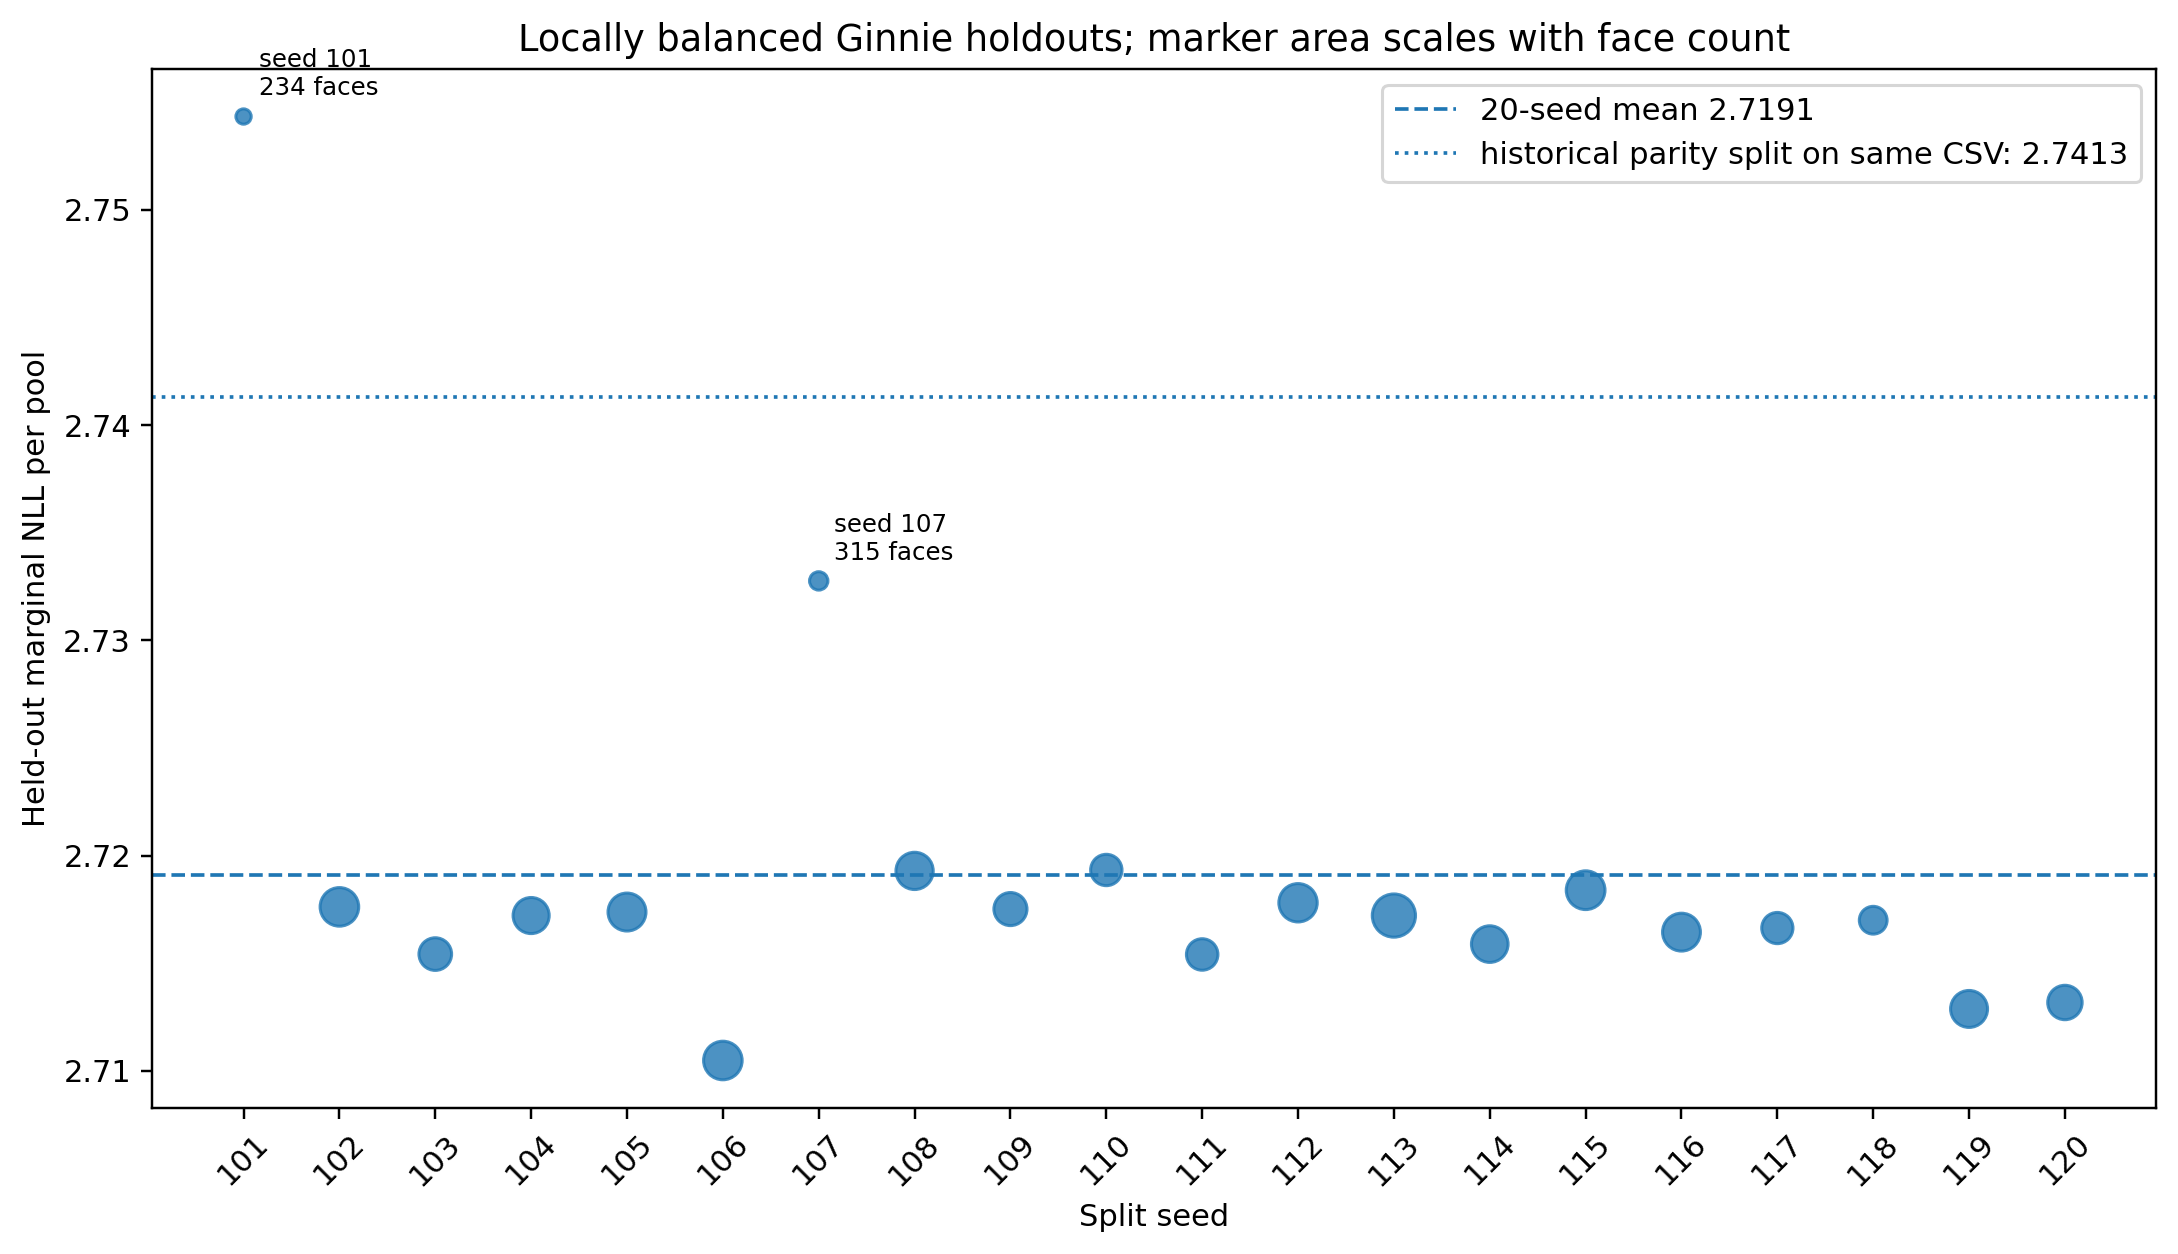
\includegraphics[width=0.92\linewidth]{bootstrap20_nll_by_seed.png}
\caption{Historical linear-child audit on twenty locally balanced Ginnie holdouts. Marker area is
proportional to final face count; seeds 101 and 107 are the two small-topology upper-tail cases. A
subsequent quadratic-child rerun rebuilds both seeds at ordinary topology sizes and returns their NLLs
to the main cluster. The dotted line is the historical parity result on the same frozen CSV.}
\label{fig:local-split-bootstrap}
\end{figure}


\subsection{Experimental geometry-generated empirical-Bayes shrinkage}
\label{sec:geometry-eb}

The locally balanced split battery exposed a second issue that is separate from false-discovery
calibration. The mesh is constructed by a split genealogy, but statistical similarity need not
follow that genealogy: two vertices can be adjacent in the final triangulation while their lowest
common split-tree ancestor is remote. The experiments in this subsection therefore keep the
adaptive topology fixed and ask whether a shrinkage layer generated from the \emph{final geometry}
can recover stable residual structure. They are conditional final-refit experiments, not changes to
the certified gate, and none is included in the July 30 code archive.

\paragraph{Quadratic inherited child target.}
The first development change replaced the linear midpoint default by inherited curvature. For an
edge with endpoints $h_0,h_1$ and exterior coarse neighbors $h_{-1},h_2$, the two-sided quadratic
prediction is
\begin{equation}\label{eq:quadratic-child-target}
 \mu_{Q}=\frac{-h_{-1}+9h_0+9h_1-h_2}{16}.
\end{equation}
Equivalently, if $\delta_{\mathrm{parent}}$ denotes the coarser midpoint surplus, then a quadratic
implies a child surplus of one quarter the parent surplus. Geometry-only conformity vertices remain
at the linear midpoint so that a topological split does not alter the fitted P1 function; only a
statistically free child is shrunk toward \eqref{eq:quadratic-child-target}. On the ten completed
non-collapse splits, this development baseline improved mean overall marginal NLL by approximately
$0.00070$ and improved nine of ten splits. Its main value was stabilization of the two historical
topology-collapse seeds rather than a direct correction of the middle-aged WAC ridges.

\paragraph{Graph-local variance sharing.}
A first geometry-generated hierarchy retained the quadratic split-tree details but estimated local
prior-variance multipliers over recursively constructed graph patches. This changed only the amount
of shrinkage, not the target value of any coefficient. Across twelve matched frozen topologies it
improved mean overall NLL by $0.000129$ (eleven of twelve splits) and the seasoned-region NLL by
$0.000043$ (twelve of twelve), while its middle-aged effect was negligible. This is evidence that
split depth alone is not the best index for the local EB scale, but it is too small to explain the
persistent ridge residuals.

\paragraph{Overlapping geometric covers and intersections.}
The larger gain came from moving the geometric hierarchy to the function level. Let $\Phi_A$ and
$\Phi_B$ be two soft graph-distance covers of the final mesh, centered to remove the intercept. Their
intersections are represented by centered products. Conditional on the frozen mesh prediction, the
residual correction is
\begin{equation}\label{eq:crossed-cover-correction}
 g(x)=\Phi_A(x)a+\Phi_B(x)b+\Phi_{AB}(x)c,
 \qquad
 a,b\sim N(0,\tau_P^2 I),\quad c\sim N(0,\tau_I^2 I).
\end{equation}
Because all components are fit jointly under the same marginal pool likelihood, overlap among the
covers enters through the likelihood Hessian rather than through a scalar effective-sample-size
correction. With twelve centers per cover, the parent effects alone improved mean overall NLL by
$0.003813$ relative to the graph-patch baseline. Adding the crossed intersections improved mean NLL
by $0.004100$ in total, with improvements in all twelve splits. The interaction increment was
$0.000287$ overall and $0.000472$ in the middle-aged band, favorable in eleven of twelve splits in
both cases.

\begin{figure}[t]
\centering
\begin{minipage}[t]{0.48\linewidth}
\centering
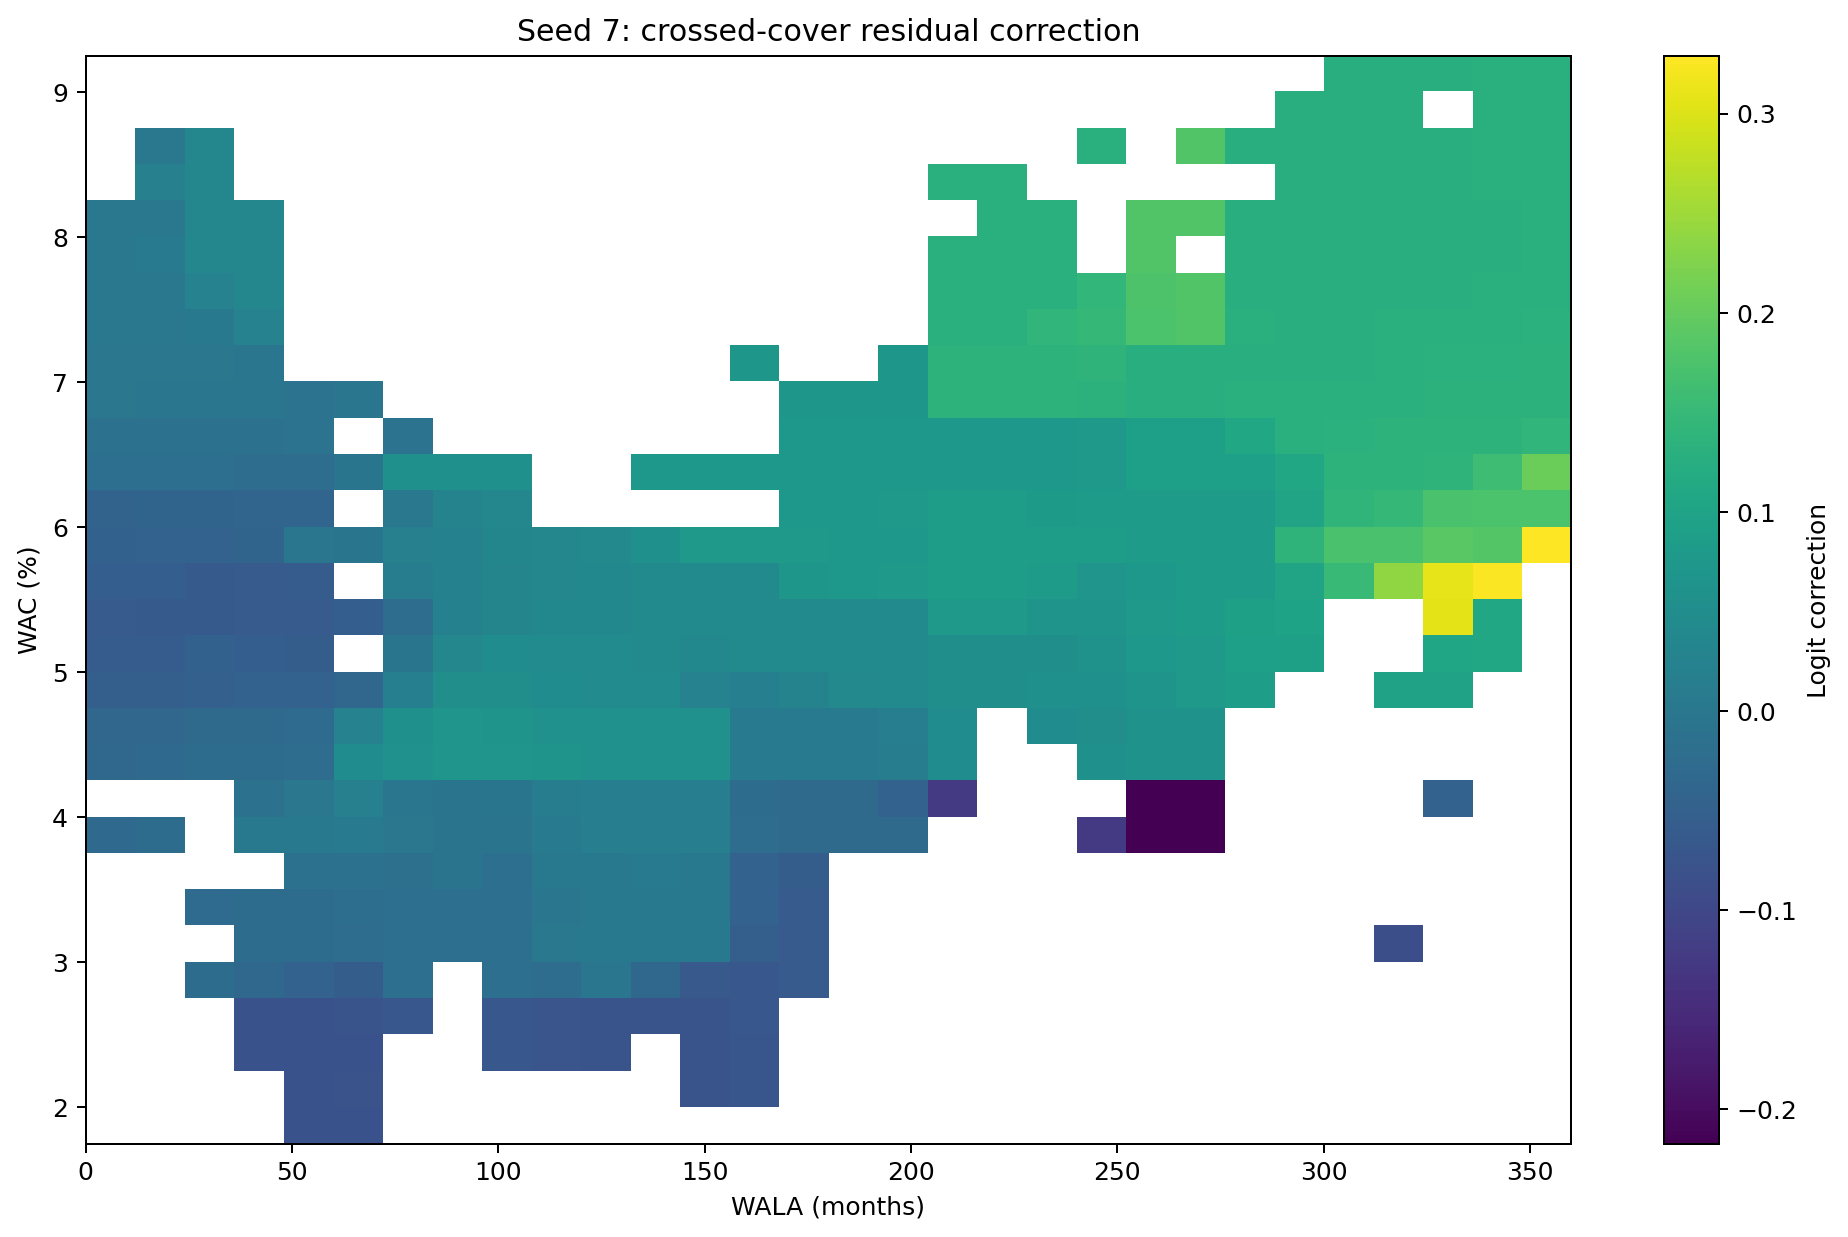
\includegraphics[width=\linewidth]{crossed_geometry_seed7_correction_field.png}
\end{minipage}\hfill
\begin{minipage}[t]{0.48\linewidth}
\centering
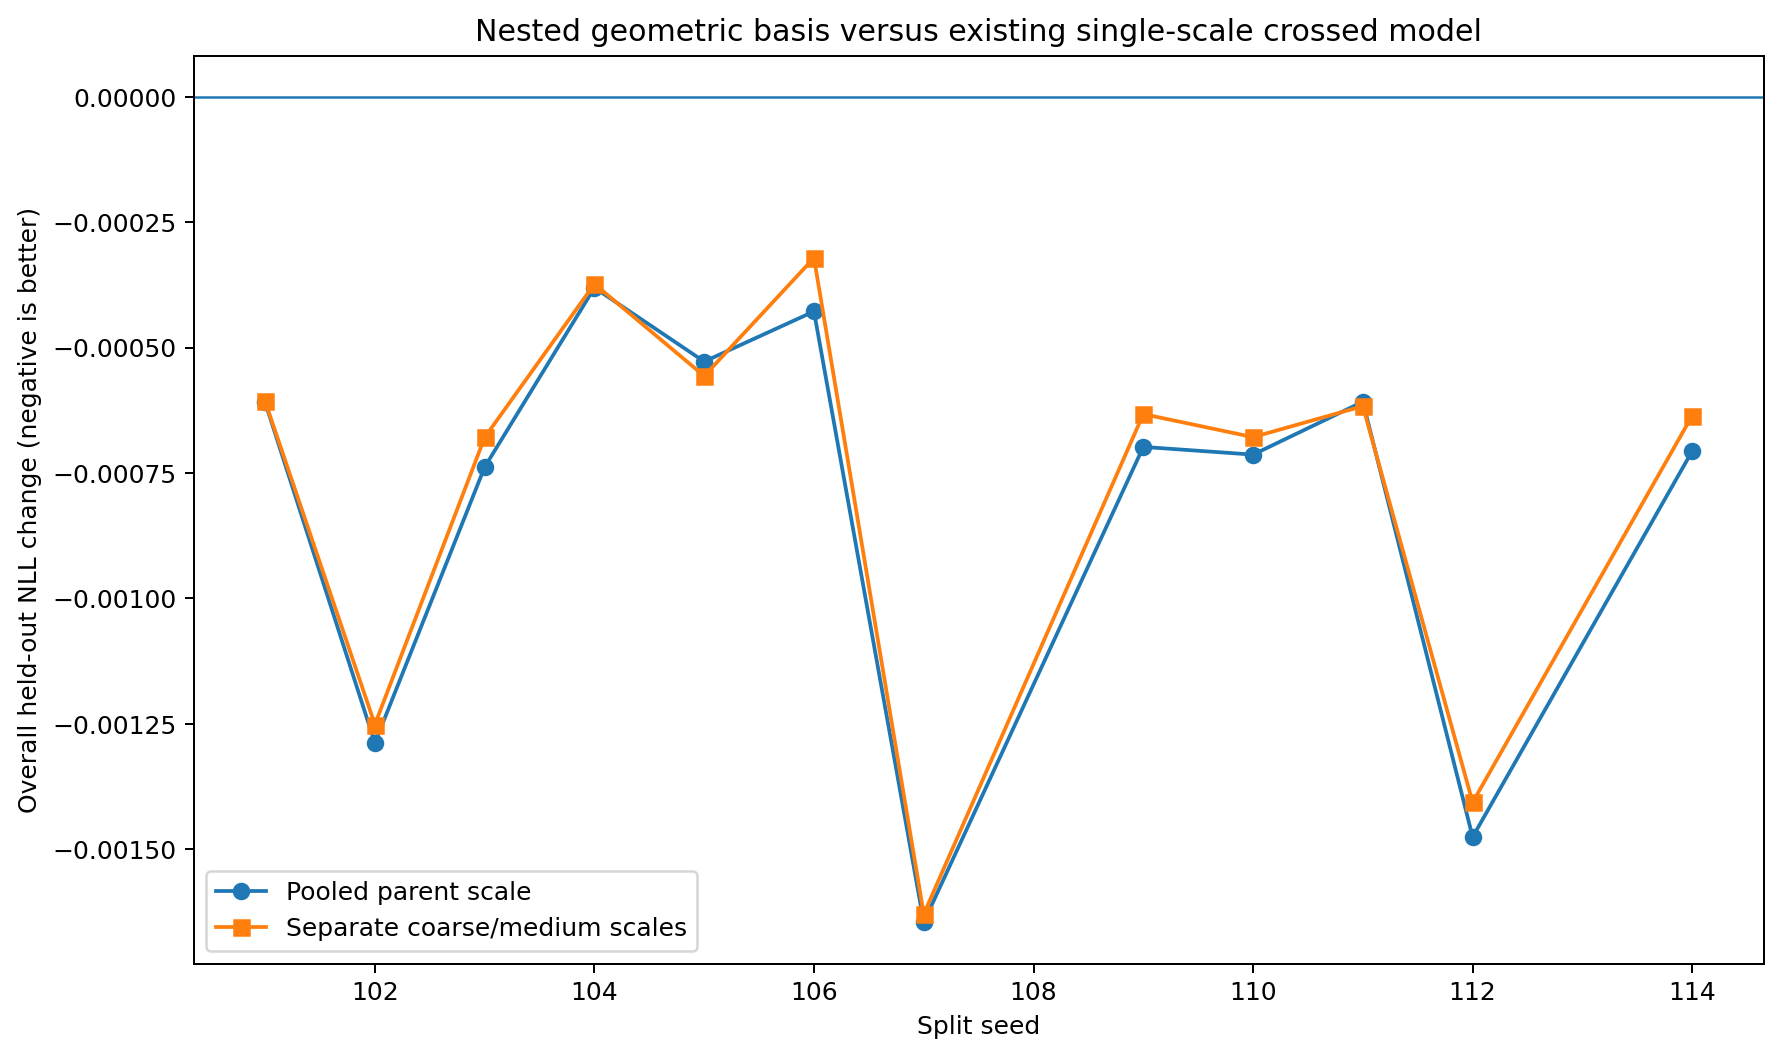
\includegraphics[width=\linewidth]{twoscale_vs_single_12seed.png}
\end{minipage}
\caption{Frozen-topology geometric correction. Left: the seed-7 crossed-cover correction on the
original WALA--WAC axes. Right: held-out overall-NLL change of the nested geometric basis relative
to the earlier single-scale crossed model; every point is below zero. The figures describe an
experimental final-refit layer and not the shipped adaptive estimator.}
\label{fig:geometry-eb-experiment}
\end{figure}

\paragraph{The smallest useful multiscale refinement.}
To separate broad spatial drift from medium-scale detail without proliferating hyperparameters, two
nested covers were constructed with six and twelve centers. The twelve-center parent basis was
projected off the six-center space under the training-information inner product, and the crossed
products were projected off both parent spaces. The preferred model is
\begin{equation}\label{eq:nested-cover-model}
 g=X_0a+X_1b+X_Ic,
 \qquad a,b\sim N(0,\tau_P^2I),\qquad c\sim N(0,\tau_I^2I),
\end{equation}
where $X_0$ is the coarse parent basis, $X_1$ is the medium parent detail, and $X_I$ is the crossed
detail. Relative to the single-scale crossed model, \eqref{eq:nested-cover-model} improved mean
overall NLL by $0.000818$ and mean middle-aged NLL by $0.000941$, with improvement in all twelve
splits. Within the nested model, the medium parent detail and crossed detail contributed mean overall
improvements of $0.000587$ and $0.000880$, respectively, each favorable in all twelve splits.

An important negative result simplifies the shrinkage law. Giving the coarse and medium parent
blocks separate EB variances made mean overall NLL worse by $0.000036$ and middle-aged NLL worse by
$0.000086$ relative to one pooled parent variance. The evidence therefore supports a multiscale
\emph{representation}, but not a distinct Gaussian variance parameter at every scale.

\paragraph{Interaction precision and the unresolved EB calculation.}
The fitted parent block retained roughly $92\%$ of its unpenalized effective degrees of freedom,
whereas the interaction block retained roughly $62\%$. A nested training-side control then held the
parent precision fixed and selected an interaction-precision multiplier from
$\{1,1/2,1/4\}$. Inner validation selected quarter precision in eleven of twelve splits. On the
untouched outer holdouts, quarter precision improved overall NLL by $0.000188$ in all twelve splits
and middle-aged NLL by $0.000234$ on average. Since the weakest tested penalty won at the boundary,
$1/4$ should not be interpreted as a structural constant or folded into the estimator.

\begin{figure}[t]
\centering
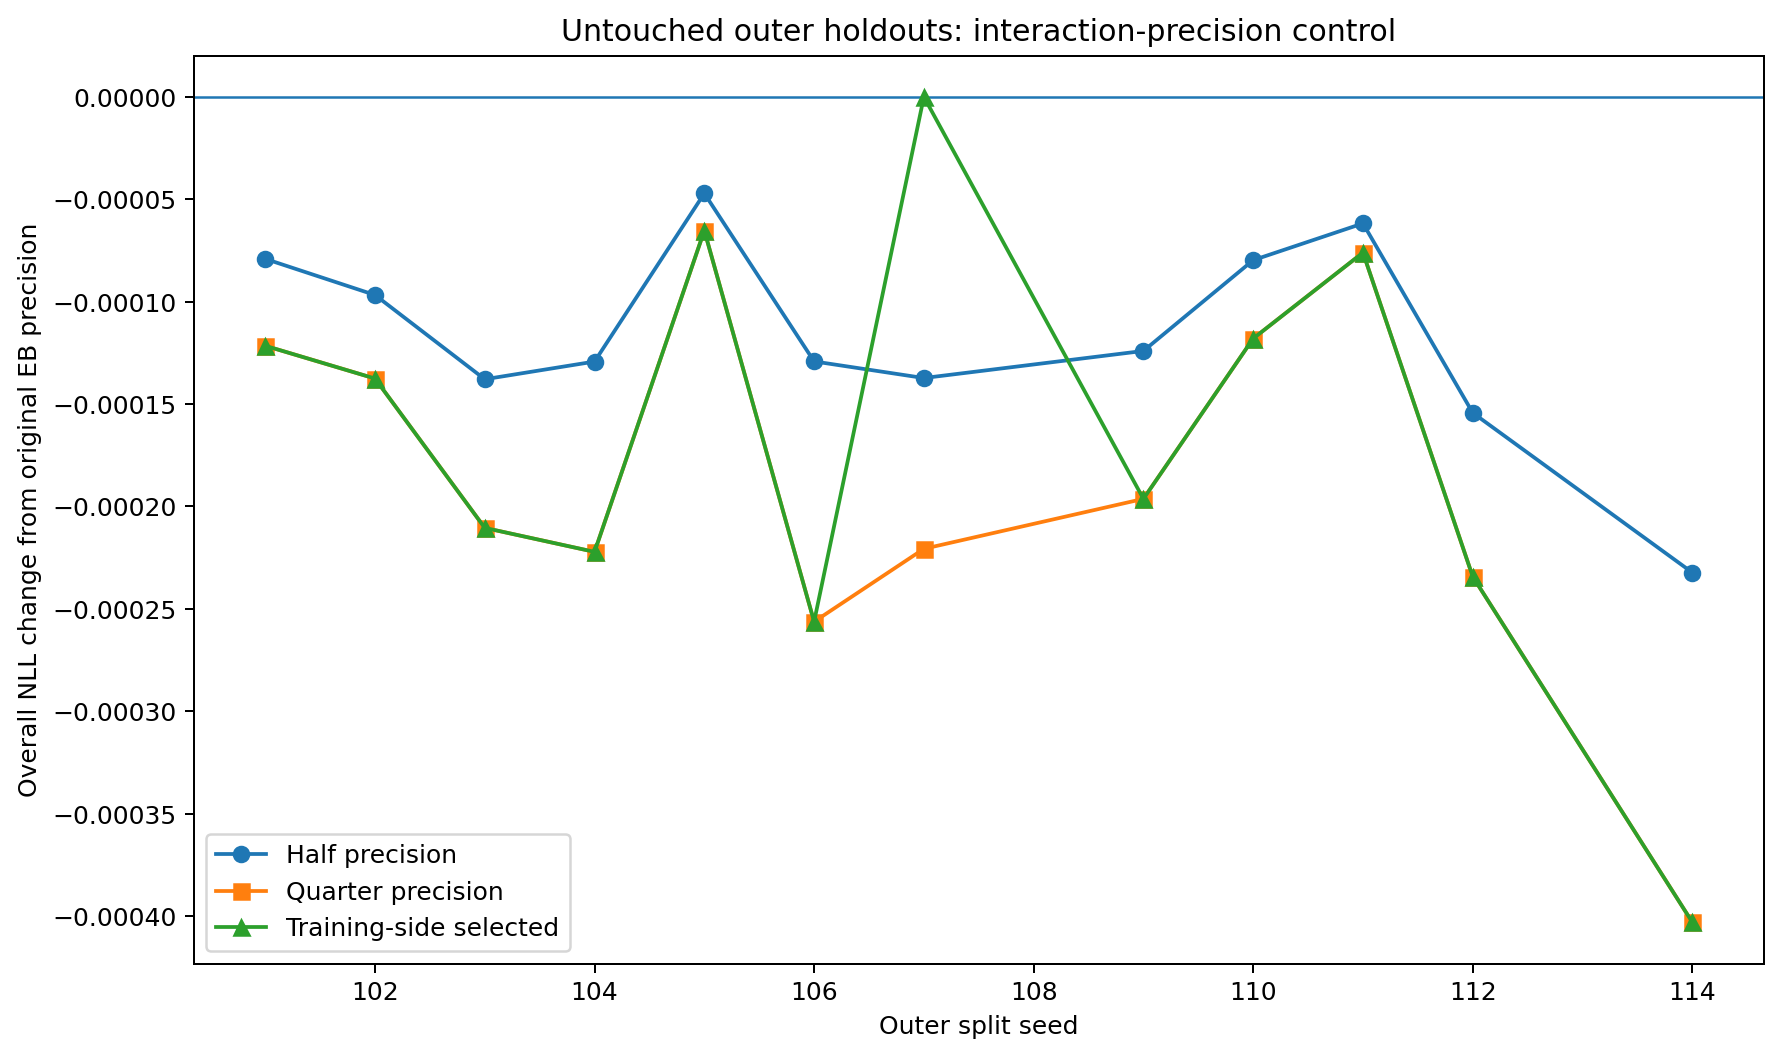
\includegraphics[width=0.82\linewidth]{interaction_precision_outer_holdout.png}
\caption{Control for the crossed-interaction precision on untouched outer holdouts. Half and quarter
precision both improve on the original EB value; quarter precision is better in every split overall.
The training-selected rule chooses quarter precision in eleven splits and the original precision in
one. The boundary optimum motivates a conditional-information EB calculation rather than adoption
of a fixed multiplier.}
\label{fig:interaction-precision-control}
\end{figure}

The principled next calculation is a joint frozen-topology fit of mesh heights, parent-cover effects,
and crossed interactions. Let $N$ denote all nuisance coordinates (mesh and parent covers) and $I$
the crossed-interaction coordinates. Partition the likelihood-plus-prior Hessian as
\[
 H=\begin{pmatrix}
 H_{NN} & H_{NI}\\
 H_{IN} & H_{II}+\lambda_I I
 \end{pmatrix}.
\]
The information available for identifying the interactions after the nuisance fit is allowed to
readjust is the Schur complement
\begin{equation}\label{eq:interaction-schur-information}
 J_I=H_{II}-H_{IN}H_{NN}^{-1}H_{NI}.
\end{equation}
Optimizing the full Laplace marginal likelihood using
$\log\det H=\log\det H_{NN}+\log\det(J_I+\lambda_I I)$ estimates the interaction precision from its
conditional information and removes the need for an arbitrary multiplier. Predictive EB on
training-side spatial folds is a fallback if corrected marginal evidence and held-out prediction
continue to disagree.

\paragraph{Exploratory directions and what survived.}
The geometry experiments also clarify several earlier negative results. Directly pooling signed
neighboring surpluses, sharing a variance only within raw WAC strips, and replacing the split
hierarchy by a full farthest-point graph hierarchy did not produce stable held-out gains. Those
failures were not evidence that geometry was irrelevant; they showed that raw surplus coordinates
have incompatible signs, orientations, and scales. Graph-patch variance sharing was modestly
positive, pairwise curvature coupling was positive but too small and ill-conditioned to justify the
cost, and function-level crossed covers were strongly positive. A second simplification also
survived: nested coarse and medium feature spaces helped, but separate Gaussian variance parameters
for the two parent scales did not. The current evidence therefore favors geometrically meaningful
function spaces with a small number of shared EB scales, rather than an elaborate coefficient-parent
system.

\paragraph{Status.}
The robust conclusion is that overlapping, nested geometric feature spaces recover a stable residual
component missed by the split-tree shrinkage. The current numerical evidence is conditional on a
frozen topology and does not establish validity under adaptive reuse of the same layer. The geometric
correction, the quarter-precision control, and the proposed Schur-complement EB calculation are
therefore documented here as development results only; the final code zip remains unchanged pending
a joint implementation, stationarity audit, and repeated outer validation.

The current status is consequently asymmetric but clear:
\begin{itemize}[leftmargin=2em,itemsep=1pt]
\item exact likelihood fitting, exact candidate profiles, and hierarchical lifecycle: implemented and
regression tested;
\item eruption prevention and boundary access: passed;
\item linear-child topology collapse on the two identified locally balanced seeds: repaired in the
quadratic-child reruns, with the full twenty-seed confirmation still pending;
\item current attribution reruns: overdispersion and omitted-shift audits reproduced; the old
$q$-U-curve and uniform frailty-bias claims revised;
\item signed-root exact gain as the candidate currency: selected and shadow validated;
\item null calibration and false-discovery certification for the exact-gain currency: failed B3 and remains open;
\item pooled-permutation direct BH: implemented in an experimental branch; passes the frozen complete-null and heavy-tailed certified-window batteries, but loses real-data power and is not adopted;
\item certified counts before the pooled-permutation subsection: legacy-gate results; the new tables are separately labeled experimental audits;
\item geometry-generated crossed-cover shrinkage: positive frozen-topology evidence, experimental
only, and excluded from the shipped release pending joint conditional-information EB.
\end{itemize}
The next experiment is the conformalized held-out gain test of
Section~\ref{sec:certnull}, not another post-hoc rescaling of the same global score family.


\begin{thebibliography}{9}\small
\bibitem{efron2004} B.~Efron, Large-scale simultaneous hypothesis testing: the choice
of a null hypothesis, \emph{JASA} 99 (2004) 96--104.
\bibitem{efron2008} B.~Efron, Microarrays, empirical Bayes and the two-groups model,
\emph{Statist.\ Sci.} 23 (2008) 1--22.
\bibitem{bh1995} Y.~Benjamini and Y.~Hochberg, Controlling the false discovery rate,
\emph{JRSS-B} 57 (1995) 289--300.
\bibitem{abramovich2006} F.~Abramovich, Y.~Benjamini, D.~Donoho, I.~Johnstone, Adapting
to unknown sparsity by controlling the false discovery rate, \emph{Ann.\ Statist.} 34
(2006) 584--653.
\bibitem{mitchell1991} W.~F.~Mitchell, Adaptive refinement for arbitrary finite-element
spaces with hierarchical bases, \emph{J.\ Comput.\ Appl.\ Math.} 36 (1991) 65--78.
\bibitem{binev2004} P.~Binev, W.~Dahmen, R.~DeVore, Adaptive finite element methods
with convergence rates, \emph{Numer.\ Math.} 97 (2004) 219--268.
\bibitem{dl1986} R.~DerSimonian and N.~Laird, Meta-analysis in clinical trials,
\emph{Controlled Clinical Trials} 7 (1986) 177--188.
\bibitem{firth1993} D.~Firth, Bias reduction of maximum likelihood estimates,
\emph{Biometrika} 80 (1993) 27--38.
\bibitem{buhlmann1967} H.~B\"uhlmann, Experience rating and credibility,
\emph{ASTIN Bulletin} 4 (1967) 199--207.
\bibitem{henderson1975} C.~R.~Henderson, Best linear unbiased estimation and
prediction under a selection model, \emph{Biometrics} 31 (1975) 423--447.
\bibitem{paule1982} R.~C.~Paule and J.~Mandel, Consensus values and weighting factors,
\emph{J.\ Res.\ Natl.\ Bur.\ Stand.} 87 (1982) 377--385.
\bibitem{efron2004pred} B.~Efron, The estimation of prediction error: covariance
penalties and cross-validation, \emph{JASA} 99 (2004) 619--632.
\bibitem{ye1998} J.~Ye, On measuring and correcting the effects of data mining and
model selection, \emph{JASA} 93 (1998) 120--131.
\bibitem{vaupel1979} J.~Vaupel, K.~Manton, E.~Stallard, The impact of heterogeneity in
individual frailty on the dynamics of mortality, \emph{Demography} 16 (1979) 439--454.
\bibitem{vovk2005} V.~Vovk, A.~Gammerman, and G.~Shafer, \emph{Algorithmic Learning in a Random
World}, Springer, 2005.
\end{thebibliography}

\end{document}
